% 高一107_曹杨二中_10月月考.tex
%   —— 高一上数学“2026-2027 年曹杨二中高一上 10 月月考”（试卷版/答案版）
% 试卷版：xelatex 高一107_曹杨二中_10月月考.tex
% 答案版：xelatex "\def\isanswer{1}% 高一107_曹杨二中_10月月考.tex
%   —— 高一上数学“2026-2027 年曹杨二中高一上 10 月月考”（试卷版/答案版）
% 试卷版：xelatex 高一107_曹杨二中_10月月考.tex
% 答案版：xelatex "\def\isanswer{1}% 高一107_曹杨二中_10月月考.tex
%   —— 高一上数学“2026-2027 年曹杨二中高一上 10 月月考”（试卷版/答案版）
% 试卷版：xelatex 高一107_曹杨二中_10月月考.tex
% 答案版：xelatex "\def\isanswer{1}% 高一107_曹杨二中_10月月考.tex
%   —— 高一上数学“2026-2027 年曹杨二中高一上 10 月月考”（试卷版/答案版）
% 试卷版：xelatex 高一107_曹杨二中_10月月考.tex
% 答案版：xelatex "\def\isanswer{1}\input{高一107_曹杨二中_10月月考.tex}"
% 紧凑版：xelatex "\def\iscompact{1}\input{高一107_曹杨二中_10月月考.tex}"
%
% 原始材料：微信公众号“魔都数学加油站”文章，作者破晓，2026-11-03 17:19 发布；
% 连载“27学年高一107”，原文标题“27学年高一107——2026-2027年上海市曹杨二中高一上10月月考”；
% 原文链接：https://mp.weixin.qq.com/s/IF4uB7aDNv-snYwbGMoDiQ。
% 正文为 10 张 PNG 页（第 1、2、4、6—9 页 4762×6735，第 3、5、10 页 2560×3620），题目下印有【解析】，为讲评版。
% 题目、解析均据原图转录；卷面水印及公众号页脚未录入。
% 第 11 题题干的三幅“出入相补”图（图 1—图 3）与第 15 题解析的三圆文氏图裁自原图、
% 去粉色水印转灰度（gao107_q11.png、gao107_q15.png），第 11 题图属题干（三版都出）、
% 第 15 题图属解析（仅答案版显示）。
%
% 卷首标题：原卷印作“2026-2027 年曹杨二中高一上 10 月月考”（公众号标题中的“上海市”
% 卷面标题行没有，本稿照卷面），年份区间按全稿惯例排 en dash；原卷未印副标题，本稿按题目内容
% 标为“集合与常用逻辑用语、不等式”。
%
% 与原卷的排版差异：
%   ① 原文从第 3 题起，填空题编号为 3—12、选择题为 13—16、解答题为 17—20，本稿保留原题号；
%   ② 原卷每题下直接印【解析】，本稿按全稿惯例将解析置于答案版；第 4 题只印【答案】另提 \ans{}；
%   ③ 原卷未印副标题，本稿按“知识模块”口径补出；
%   ④ 原卷填空横线按全稿惯例排为 \blankline[4.4em]；解答题按惯例加 \ansspace；选择题括号排
%      \mbox{（\quad）}、选项段前按惯例加 \keepwithprev；
%   ⑤ 原卷数集字母粗体与斜体混用（第 3 题 $\mathbf{R}$、第 4 题斜体 $R$、第 16 题粗体
%      $\mathbf{Z}$、$\mathbf{Q}$ 等），按全稿惯例统一改 \R、\Z、\Q。
%
% 原卷存疑：第 10 题解析“由 $\Delta=16m^2-8(2m^2+3m-2)\geqslant0$ 得 $m\leqslant\dfrac23$”
% 行末原卷无句读，照录。第 16 题解析②“取 $A=[-1,1]$，$B=[-2,2]$，$A$ 是 $B$ 的
% $\dfrac12$-邻集，但反之不成立”，据以判①真②假，照录。
%
% 行数核对：逐题数 \step/\stepm 条数，合计 112 条（Q3：5；Q4：0；Q5：2；Q6：2；Q7：2；
% Q8：4；Q9：8；Q10：4；Q11：9；Q12：3；Q13：5；Q14：3；Q15：12；Q16：5；Q17：15；
% Q18：6；Q19：15；Q20：12），与原卷印刷行逐题相等。第 4 题只印【答案】，提 \ans{}，
% 不计入 \step 账。
%
\documentclass[a4paper,11pt]{article}
\usepackage{common}

\begin{document}

\examtitlest[3]{2026--2027 年曹杨二中高一上 10 月月考}{集合与常用逻辑用语、不等式}

\bigsec{一、填空题}

\begin{enumerate}
\setcounter{enumi}{2}

\item 设 $a\in\R$，若 $3\in\{\sqrt3,a^2,a\}$，则 $a=$\blankline[4.4em].

\ifanswer
\solbegin
\step{因为 $3\in\{\sqrt3,a^2,a\}$，所以 $a^2=3$，解得 $a=\sqrt3$ 或 $a=-\sqrt3$,}
\step{当 $a=\sqrt3$ 时，集合为 $\{\sqrt3,3,\sqrt3\}$，不满足集合元素的互异性，舍去；}
\step{当 $a=-\sqrt3$ 时，集合为 $\{\sqrt3,3,-\sqrt3\}$，符合要求；}
\step{若 $a=3$，此时集合为 $\{\sqrt3,9,3\}$，符合要求；}
\step{综上，$a$ 为 $-\sqrt3$ 或 $3$.}
\solend
\fi

\item 设 $a\in\R$，已知集合 $A=\{x\mid x\leqslant a\}$，$B=\{x\mid x>2\}$. 若 $A\cup B=\R$，则 $a$ 的取值范围是\blankline[4.4em].

\ifanswer
\ans{$a\geqslant2$}
\fi

\item 设 $x>0$，$y>0$ 且 $x+3y=1$，则 $xy$ 的最大值为\blankline[4.4em].

\ifanswer
\solbegin
\step{由于 $x>0$，$y>0$ 且 $x+3y=1$，则 $1=x+3y\geqslant2\sqrt{3xy}$，得 $xy\leqslant\dfrac1{12}$,}
\step{当且仅当 $x=3y=\dfrac12$ 时取等号，则 $xy$ 的最大值为 $\dfrac1{12}$.}
\solend
\fi

\item 设 $a\in\R$，若集合$\left\{x\,\middle|\,\dfrac{ax}{x-1}=x\right\}$有且仅有两个子集，则 $a=$\blankline[4.4em].

\ifanswer
\solbegin
\step{由 $\dfrac{ax}{x-1}=x$ 得 $ax=x(x-1)$，即 $x(x-a-1)=0$,}
\step{所以此方程有两个相等的（不等于 1）的实数根或有一根为 1，所以 $a=-1$ 或 $0$.}
\solend
\fi

\item 已知全集 $U=\{x\mid x^2-8x-20<0\}$，集合 $A=\{x\mid 1-x^2>0$ 且 $x<0\}$，则 $\overline A=$\blankline[4.4em].

\ifanswer
\solbegin
\step{$U=\{x\mid-2<x<10\}$，$A=\{x\mid-1<x<0\}$,}
\step{所以 $\overline A=\{x\mid-2<x\leqslant-1$ 或 $0\leqslant x<10\}$.}
\solend
\fi

\item 设 $a,b\in\R$，若不等式 $-x^2-ax+b\geqslant0$ 的解集为 $[-2,3]$，则不等式 $\lvert ax+b\rvert<5$ 的解集为\blankline[4.4em].

\ifanswer
\solbegin
\step{由不等式 $-x^2-ax+b\geqslant0$ 的解集为 $[-2,3]$,}
\step{得 $-2$、$3$ 是方程 $-x^2-ax+b=0$ 的两个根，所以 $a=-1$，$b=6$.}
\step{解不等式 $\lvert-x+6\rvert<5$，得 $-5<x-6<5$，解得 $1<x<11$,}
\step{即所求不等式的解集为 $(1,11)$.}
\solend
\fi

\item 某货运卡车以 $x$ 千米／时的速度匀速行驶 300 千米，按交通法规限制 $50\leqslant x\leqslant100$，假设
柴油的价格为每升 6 元，汽车每小时耗油 $\left(4+\dfrac{x^2}{420}\right)$ 升，司机工资为每小时 46 元. 则当
$x=$\blankline[4.4em]（千米／时），这次行车的总费用（油费与司机工资的总和）最低.

\ifanswer
\solbegin
\step{因为卡车行驶 300 千米，速度为 $x$ 千米／时,}
\step{因此总用时为 $t=\dfrac{300}{x}$ 小时，其中 $50\leqslant x\leqslant100$,}
\step{每小时油费为 $6\cdot\left(4+\dfrac{x^2}{420}\right)$ 元，每小时司机工资为 46 元，因}
\step{此每小时总支出为 $6\cdot\left(4+\dfrac{x^2}{420}\right)+46=70+\dfrac{x^2}{70}$ 元.}
\step{设全程总费用为 $y$，则 $y=\dfrac{300}{x}\cdot\left(70+\dfrac{x^2}{70}\right)=\dfrac{21000}{x}+\dfrac{30x}{7}$,}
\step{因为 $50\leqslant x\leqslant100$，$\dfrac{21000}{x}+\dfrac{30x}{7}\geqslant2\sqrt{\dfrac{21000}{x}\cdot\dfrac{30x}{7}}=600$,}
\step{当且仅当 $\dfrac{21000}{x}=\dfrac{30x}{7}$，即 $x=70$ 时取等号，且 $70\in[50,100]$,}
\step{因此当 $x=70$ 千米／时，行车的总费用（油费与司机工资的总和）最低.}
\solend
\fi

\item 设 $x_1$、$x_2$ 是关于 $x$ 的方程 $2x^2-4mx+2m^2+3m-2=0$ 的两个实数根，则 $x_1^2+x_2^2$ 的最小值为\blankline[4.4em].

\ifanswer
\solbegin
\step{由题意得 $x_1+x_2=2m$，$x_1x_2=m^2+\dfrac{3m}{2}-1$,}
\step{由 $\Delta=16m^2-8(2m^2+3m-2)\geqslant0$ 得 $m\leqslant\dfrac23$}
\step{所以 $x_1^2+x_1^2=(x_1+x_2)^2-2x_1x_2=4m^2-2m^2+3m+2=2m^2-3m+2$,% 原卷左端作 x_1²+x_1²，照录
}
\step{结合二次函数的性质得，当 $m=\dfrac23$ 时取得最小值 $\dfrac89$.}
\solend
\fi

\item 小玲在钻研《九章算术》中“勾股容方”问题“今有勾五步，股十二步，问勾中容方几
何？”时，发现魏晋时期数学家刘徽在其《九章算术注》中利用出入相补原理给出了这个
问题的一般解法：如图 1，用对角线将长和宽分别为 $b$ 和 $a$ 的矩形分成两个直角三角形，
每个直角三角形再分成一个内接正方形（黄）和两个小直角三角形（朱、青）. 将三种颜色
的图形进行重组，得到如图 2 所示的矩形，该矩形长为 $a+b$，宽为内接正方形的边长
$d$. 由刘徽构造的图形可以得到许多重要的结论，如图 3，设 $D$ 为斜边 $BC$ 的中点，作直
角三角形 $ABC$ 的内接正方形对角线 $AE$，过点 $A$ 作 $AF\perp BC$ 于点 $F$，则下列四个推理中
正确的序号是\blankline[4.4em].

\begin{center}
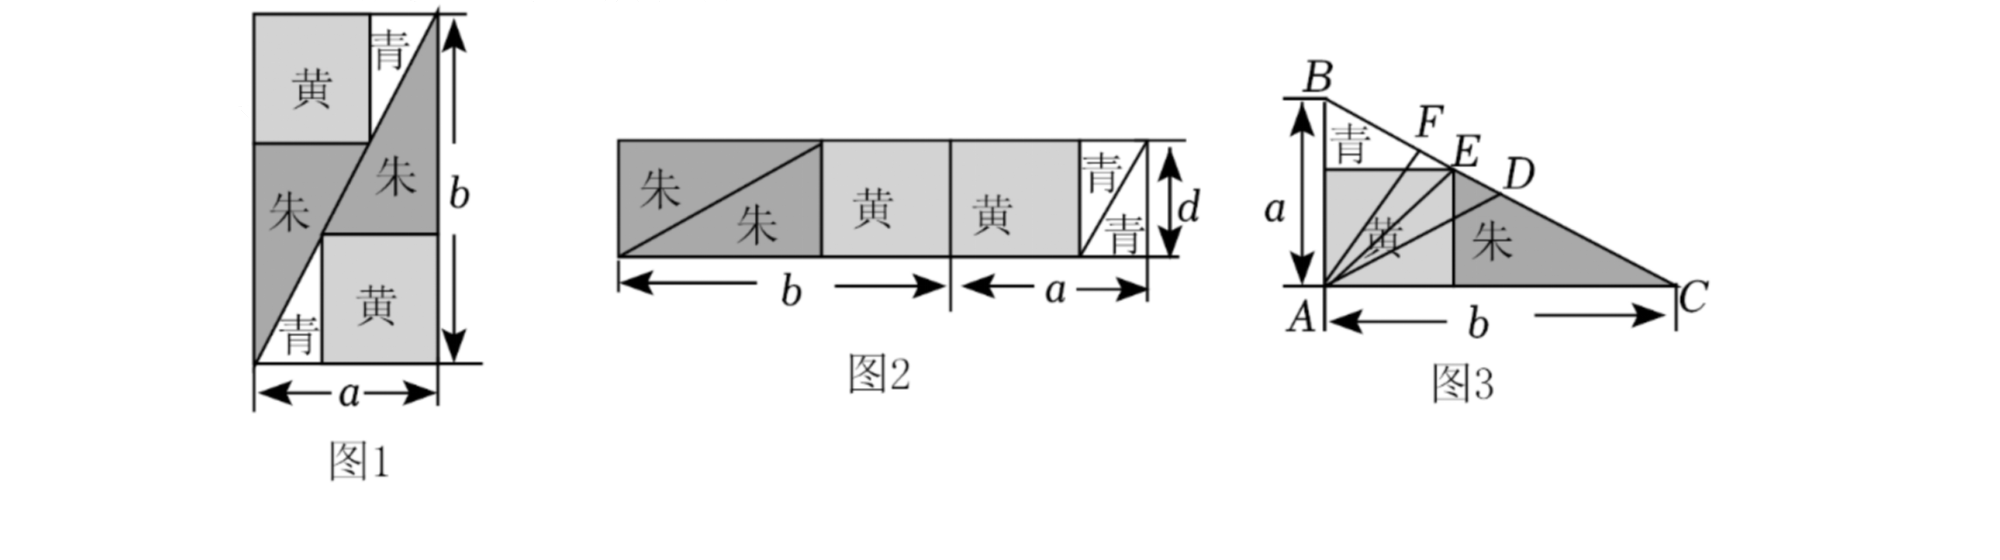
\includegraphics[width=0.86\textwidth]{figures/gao107_q11.png}
\end{center}

①由图 1 和图 2 面积相等得 $d=\dfrac{2ab}{a+b}$　　②由 $AE\geqslant AF$ 可得 $\sqrt{\dfrac{a^2+b^2}2}\geqslant\dfrac{a+b}2$

③由 $AD\geqslant AE$ 可得 $\sqrt{\dfrac{a^2+b^2}2}\geqslant\dfrac{2}{\dfrac1a+\dfrac1b}$　④由 $AD\geqslant AF$ 可得 $a^2+b^2\geqslant2ab$

\ifanswer
\solbegin
\step{对于①，由图 1 和图 2 面积相等得 $ab=(a+b)\times d$，所以 $d=\dfrac{ab}{a+b}$，故①错,}
\step{对于②，因为 $AF\perp BC$，所以 $\dfrac12ab=\dfrac12\sqrt{a^2+b^2}\times AF$,}
\step{所以 $AF=\dfrac{ab}{\sqrt{a^2+b^2}}$，$AE=\sqrt2d=\dfrac{\sqrt2ab}{a+b}$,}
\step{因为 $AE\geqslant AF$，所以 $\dfrac{\sqrt2ab}{a+b}\geqslant\dfrac{ab}{\sqrt{a^2+b^2}}$，整理得 $\sqrt{\dfrac{a^2+b^2}2}\geqslant\dfrac{a+b}2$，故②对,}
\step{对于③，因为 $D$ 是斜边 $BC$ 的中点，所以 $AD=\sqrt{\dfrac{a^2+b^2}2}$,}
\step{因为 $AD\geqslant AE$，所以 $\sqrt{\dfrac{a^2+b^2}2}\geqslant\dfrac{\sqrt2ab}{a+b}$，整理得 $\sqrt{\dfrac{a^2+b^2}2}\geqslant\dfrac{2}{\dfrac1a+\dfrac1b}$，故③对,}
\step{对于④，因为 $AD\geqslant AF$，所以 $\sqrt{\dfrac{a^2+b^2}2}\geqslant\dfrac{ab}{\sqrt{a^2+b^2}}$，整理得 $a^2+b^2\geqslant2ab$,}
\step{故④对,}
\step{故正确的是②③④.}
\solend
\fi

\item 设 $a,b,c,d\in\R$ 且$\lvert a-b\rvert\leqslant2$,$\lvert c-d\rvert\leqslant2$,$\lvert a\rvert\leqslant3$,$\lvert c\rvert\leqslant3$，则 $\lvert ad-bc\rvert$ 的最大值为\blankline[4.4em].% 原卷四处条件间均排半角逗号，照录

\ifanswer
\solbegin
\step{令 $a-b=e$,$c-d=f$，则 $\lvert e\rvert\leqslant2$,$\lvert f\rvert\leqslant2$,$\lvert a\rvert\leqslant3$,$\lvert c\rvert\leqslant3$}
\step{则 $\lvert ad-bc\rvert=\lvert a(c-f)-(a-e)c\rvert=\lvert ce-af\rvert\leqslant\lvert c\rvert\,\lvert e\rvert+\lvert a\rvert\,\lvert f\rvert\leqslant12$,}
\step{则 $\lvert ad-bc\rvert$ 的最大值为 12.}
\solend
\fi

\end{enumerate}

\bigsec{二、选择题}

\begin{enumerate}
\setcounter{enumi}{12}

\item 下列说法正确的是\mbox{（\quad）}

\keepwithprev
A. 若 $a>b>0$，则 $ac^2>bc^2$\qquad\qquad B. 若 $a<b<0$，则 $a^2>ab>b^2$

C. 若 $a>b$，则 $a^2>b^2$\qquad\qquad\qquad D. 若 $a<b$，则 $\dfrac1a>\dfrac1b$

\ifanswer
\solbegin
\step{$A$. 当 $a>b>0$ 时，取 $c=0$，则 $ac^2>bc^2$ 不成立，故 $A$ 错误；}
\step{$B$. 当 $a<b<0$ 时，由不等式的基本性质得 $a^2>ab>b^2>0$，故 $B$ 正确；}
\step{$C$. 当 $a>b$ 时，取 $a=0$，$b=-1$，则 $a^2>b^2$ 不成立，故 $C$ 错误；}
\step{$D$. 当 $a<b$ 时，取 $a=0$，$b=1$，则 $\dfrac1a>\dfrac1b$ 不成立，故 $D$ 错误.}
\step{故选 $B$.}
\solend
\fi

\item 小玲在学习《论语·子路》读到“其身正，不令而行；其身不正，虽令不从”，这句话的
数学含义可以理解为：“身正”是“令行”的\mbox{（\quad）}

\keepwithprev
A. 充分非必要条件\qquad\qquad B. 必要不充分条件

C. 充要条件\qquad\qquad\qquad D. 既非充分又非必要条件

\ifanswer
\solbegin
\step{其身正，不令而行，即身正$\Rightarrow$令行，所以“身正”是“令行”的充分条件；}
\step{又其身不正，虽令不从，即令行$\Rightarrow$身正，所以“身正”是“令行”的必要条件；}
\step{综上，“身正”是“令行”的充要条件. 故选 $C$.}
\solend
\fi

\item 某地对农户抽样调查，结果如下：电冰箱拥有率为 $45\%$，电视机拥有率为 $55\%$，洗衣
机拥有率为 $65\%$，拥有上述三种电器的任意两种的占 $35\%$，三种电器齐全的为 $25\%$，那
么一种电器也没有的农户所占比例是\mbox{（\quad）}

\keepwithprev
A. $12\%$\qquad B. $15\%$\qquad C. $18\%$\qquad D. $20\%$

\ifanswer
\solbegin
\step{设只有电冰箱和电视机的农户有 $a$ 家，只有电冰箱和洗衣机的农户有 $b$ 家,}
\step{只有洗衣机和电视机的农户有 $c$ 家,}
\step{只有电视机、电冰箱、洗衣机的分别有 $d$、$e$、$f$ 家,}
\step{没有任何电器的农户有 $x$ 家,}

\begin{center}
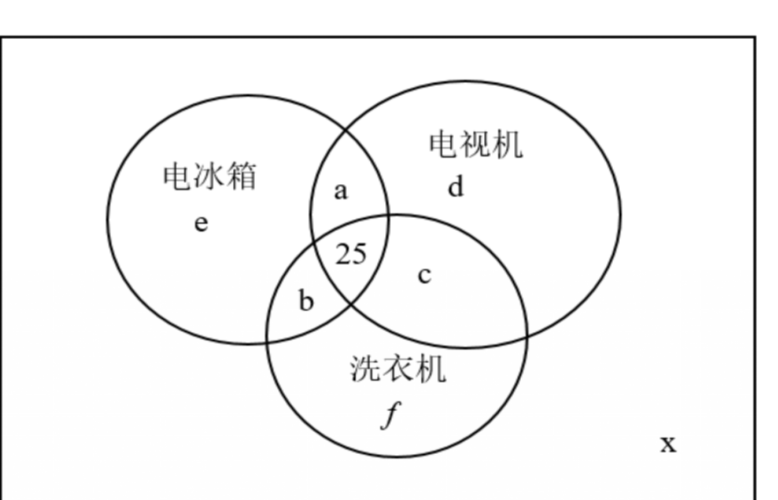
\includegraphics[width=0.42\textwidth]{figures/gao107_q15.png}
\end{center}

\step{所以 $25+a+b+e=45$①，$25+a+c+d=55$②,}
\step{$25+b+c+f=65$③,}
\step{把上面三个式子相加得 $2(a+b+c)+d+e+f=90$④,}
\step{对于拥有上述三种电器的任意两种的占 $35\%$，得 $a+b+c=35$⑤,}
\step{把⑤代入④可得到 $d+e+f=20$⑥,}
\step{因为农户共有 100 家，所以 $25+a+b+c+d+e+f+x=100$,}
\step{把⑤和⑥代入上式得 $x=20$，即一种电器也没有的农户所占比例为 $20\%$.}
\step{故选 $D$.}
\solend
\fi

\item 设 $d>0$，已知 $A,B$ 是两个数集. 若对任意 $x\in A$，都存在 $y\in B$，使得 $\lvert x-y\rvert<d$，则
称 $A$ 是 $B$ 的一个“$d-$邻集”. 现有下列两个命题：① $M=\{a+b\sqrt2\mid a,b\in\Z\}$ 是 $\Q$ 的一个
$\dfrac1{2025}$
一邻集；②若 $A$ 是 $B$ 的一个 $d-$邻集，则 $B$ 也是 $A$ 的一个 $d-$邻集；则\mbox{（\quad）}% 原卷把 d−邻集 的连字符断行后排成“一邻集”，照录

\keepwithprev
A. ①真②假\qquad B. ①假②真\qquad C. ①真②真\qquad D. ①假②假

\ifanswer
\solbegin
\step{对于①，任取 $M$ 中的元素 $x_0=a_0+b_0\sqrt2$,}
\step{则存在 $y_0\in\Q\cap\left(a_0+b_0\sqrt2-\dfrac1{2025},a_0+b_0\sqrt2+\dfrac1{2025}\right)$ 满足题意，故①正确；}
\step{对于②，取 $A=[-1,1]$,$B=[-2,2]$, $A$ 是 $B$ 的 $\dfrac12-$邻集，但反之不成立,}
\step{故②错误；}
\step{故选 $A$.}
\solend
\fi

\end{enumerate}

\bigsec{三、解答题}

\begin{enumerate}
\setcounter{enumi}{16}

\item 设 $a\in\R$，完成下列问题：

（1）求不等式 $3(a+1)x-3>2ax-3a$ 的解集 $M$；

（2）设集合 $A=\{x\mid x^2-ax+a^2-19=0\}$，$B=\{x\mid x^2-5x+6=0\}$，
$C=\{x\mid x^2+2x-8=0\}$. 若 $A\cap B\supset\varnothing$，$A\cap C=\varnothing$，求 $a$ 的值.

\ifanswer
\solbegin
\step{（1）不等式 $3(a+1)x-3>2ax-3a$ 可化为 $(a+3)x>3-3a$,}
\step{当 $a+3>0$，即 $a>-3$ 时，解得 $x>\dfrac{3-3a}{a+3}$,}
\step{当 $a+3=0$，即 $a=-3$ 时，不等式化为 $0\cdot x>12$，无解,}
\step{当 $a+3<0$，即 $a<-3$ 时，解得 $x<\dfrac{3-3a}{a+3}$,}
\step{综上所述，当 $a>-3$ 时，$M=\left(\dfrac{3-3a}{a+3},+\infty\right)$；}
\step{当 $a=-3$ 时，$M=\varnothing$；}
\step{当 $a<-3$ 时，$M=\left(-\infty,\dfrac{3-3a}{a+3}\right)$；}
\step{（2）$B=\{x\mid x^2-5x+6=0\}=\{2,3\}$，$C=\{x\mid x^2+2x-8=0\}=\{2,-4\}$,}
\step{因为 $A\cap B\supset\varnothing$，所以 $A\cap B\neq\varnothing$，又因为 $A\cap C=\varnothing$,}
\step{所以 $3\in A$，$2\notin A$，$-4\notin A$,}
\step{把 $x=3$ 代入方程 $x^2-ax+a^2-19=0$ 得 $9-3a+a^2-19=0$,}
\step{解得 $a=-2$ 或 $a=5$,}
\step{当 $a=-2$ 时，集合 $A=\{x\mid x^2+2x-15=0\}=\{3,-5\}$，符合题意,}
\step{当 $a=5$ 时，集合 $A=\{x\mid x^2-5x+6=0\}=\{3,2\}$，不符合题意，舍去,}
\step{综上所述，$a$ 的值为 $-2$.}
\solend
\fi

\item 完成下列问题：

（1）设 $x$、$y\in\R$，且 $x+y>5$，用反证法证明：$x>3$ 或 $y>2$；

（2）设 $x>0$，$a=x+1$，$b=\sqrt{x^2+7x+1}$，求 $\dfrac ba$ 的最大值.

\ifanswer
\solbegin
\step{（1）假设 $x\leqslant3$ 且 $y\leqslant2$，则 $x+y\leqslant3+2=5$，这与已知 $x+y>5$ 矛盾,}
\step{故 $x>3$ 或 $y>2$；}
\step{（2）$x>0$，$a=x+1$，$b=\sqrt{x^2+7x+1}$,}
\step{则 $\dfrac ba=\dfrac{\sqrt{x^2+7x+1}}{x+1}=\sqrt{\dfrac{x^2+7x+1}{x^2+2x+1}}=\sqrt{\dfrac{x^2+2x+1+5x}{x^2+2x+1}}$}
\step{$=\sqrt{1+\dfrac{5x}{x^2+2x+1}}=\sqrt{1+\dfrac{5}{x+\dfrac1x+2}}\leqslant\sqrt{1+\dfrac{5}{2\sqrt{x\cdot\dfrac1x}+2}}=\dfrac32$,}
\step{当且仅当 $x=\dfrac1x$，即 $x=1$ 时取等号，故 $\dfrac ba$ 的最大值为 $\dfrac32$.}
\solend
\fi

\item 已知函数 $f(x)=\lvert2x-a\rvert+a$.

（1）当 $a=2$ 时，求不等式 $f(x)\leqslant6+\lvert x+2\rvert$ 的解集；

（2）设 $g(x)=\lvert2x-1\rvert$，若不等式 $f(x)+g(x)\geqslant3$ 对一切 $x\in\R$ 恒成立，求实数 $a$ 的取值
范围.

\ifanswer
\solbegin
\ansspace*
\step{（1）$a=2$ 时，$f(x)=\lvert2x-2\rvert+2$,}
\step{则 $f(x)\leqslant6+\lvert x+2\rvert\Leftrightarrow\lvert2x-2\rvert+2\leqslant6+\lvert x+2\rvert$，即 $\lvert2x-2\rvert-\lvert x+2\rvert\leqslant4$,}
\step{当 $x<-2$ 时，$2-2x+x+2\leqslant4$，解得 $x\geqslant0$，与 $x<-2$ 取交集得 $\varnothing$,}
\step{当 $-2\leqslant x\leqslant1$ 时，$2-2x-x-2\leqslant4$，解得 $x\geqslant-\dfrac43$,}
\step{与 $-2\leqslant x\leqslant1$ 取交集得 $-\dfrac43\leqslant x\leqslant1$,}
\step{当 $x>1$ 时，$2x-2-x-2\leqslant4$，解得 $x\leqslant8$，与 $x>1$ 取交集得 $1<x\leqslant8$,}
\step{综上，不等式 $f(x)\leqslant6+\lvert x+2\rvert$ 的解集为 $\left\{x\,\middle|\,-\dfrac43\leqslant x\leqslant8\right\}$；}
\step{（2）$f(x)+g(x)\geqslant3$，即 $\lvert2x-a\rvert+a+\lvert2x-1\rvert\geqslant3$,}
\step{故 $\lvert2x-a\rvert+\lvert2x-1\rvert\geqslant3-a$,}
\step{当 $a\geqslant3$ 时，不等式显然成立,}
\step{当 $a<3$ 时,}
\step{由三角不等式得 $\lvert2x-a\rvert+\lvert2x-1\rvert\geqslant\lvert2x-a-(2x-1)\rvert=\lvert1-a\rvert$,}
\step{当且仅当 $(2x-a)(2x-1)\leqslant0$ 时取等号，因此 $\lvert1-a\rvert\geqslant3-a$,}
\step{平方得 $(1-a)^2\geqslant(3-a)^2$，解得 $a\geqslant2$，故 $2\leqslant a<3$.}
\step{综上，实数 $a$ 的取值范围是 $a\geqslant2$.}
\solend
\fi

\item 对于集合 $A,B$，定义集合 $A-B=\{x\mid x\in A$ 且 $x\notin B\}$.

（1）若 $A=\{1,2,3,4\}$,$B=\{3,4,5\}$，求集合 $A-B$ 和 $B-A$；

（2）给定集合 $A,B$，求所有满足方程组
\[
\begin{cases}
X\cap(A\cup B)=X\\
A\cap(B\cup X)=A\\
B\cap(A\cup X)=B\\
X\cap(A\cap B)=\varnothing
\end{cases}
\]
的集合 $X$（用 $A,B$ 表示）；

（3）用 $\lvert M\rvert$ 表示集合 $M$ 中的元素个数. 给定正整数 $n$，集合 $S=\{1,2,\cdots,n\}$. 对于实数
集的非空有限子集 $A,B$，定义集合 $C=\{x\mid x=a+b,a\in A,b\in B\}$. 求证：

$\lvert A-S\rvert+\lvert B-S\rvert+\lvert S-C\rvert\geqslant1$.

\ifanswer
\solbegin
\step{（1）由 $A=\{1,2,3,4\}$,$B=\{3,4,5\}$，则 $A-B=\{1,2\}$,$B-A=\{5\}$；}
\step{（2）由
$\begin{cases}
X\cap(A\cup B)=X\\
X\cap(A\cap B)=\varnothing
\end{cases}$，
得 $X\subseteq A-B$ 或 $X\subseteq B-A$,}
\step{再结合
$\begin{cases}
A\cap(B\cup X)=A\\
B\cap(A\cup X)=B
\end{cases}$，
得 $X=(A-B)\cup(B-A)$,}
\step{所以 $X=(A-B)\cup(B-A)$；}
\step{（3）$\lvert X\rvert$ 表示集合 $X$ 中的元素个数，则 $\lvert X\rvert\geqslant0$,}
\step{若 $A\cup B$ 中至少含有一个不在 $S$ 中的元素，则 $\lvert A-S\rvert+\lvert B-S\rvert\geqslant1$,}
\step{即 $\lvert A-S\rvert+\lvert B-S\rvert+\lvert S-C\rvert\geqslant1$.}
\step{若 $A\subseteq S$，且 $B\subseteq S$，则 $\lvert A-S\rvert=\lvert B-S\rvert=0$.}
\step{此时 $A$ 中最小的元素 $a\geqslant1$,$B$ 中最小的元素 $b\geqslant1$.}
\step{所以 $C$ 中最小的元素 $a+b\geqslant2$，则 $1\notin C$,}
\step{因为 $S=\{1,2,\cdots,n\}$，所以 $\lvert S-C\rvert\geqslant1$，即 $\lvert A-S\rvert+\lvert B-S\rvert+\lvert S-C\rvert\geqslant1$.}
\step{综上所述，$\lvert A-S\rvert+\lvert B-S\rvert+\lvert S-C\rvert\geqslant1$.}
\solend
\fi

\end{enumerate}

\end{document}
"
% 紧凑版：xelatex "\def\iscompact{1}% 高一107_曹杨二中_10月月考.tex
%   —— 高一上数学“2026-2027 年曹杨二中高一上 10 月月考”（试卷版/答案版）
% 试卷版：xelatex 高一107_曹杨二中_10月月考.tex
% 答案版：xelatex "\def\isanswer{1}\input{高一107_曹杨二中_10月月考.tex}"
% 紧凑版：xelatex "\def\iscompact{1}\input{高一107_曹杨二中_10月月考.tex}"
%
% 原始材料：微信公众号“魔都数学加油站”文章，作者破晓，2026-11-03 17:19 发布；
% 连载“27学年高一107”，原文标题“27学年高一107——2026-2027年上海市曹杨二中高一上10月月考”；
% 原文链接：https://mp.weixin.qq.com/s/IF4uB7aDNv-snYwbGMoDiQ。
% 正文为 10 张 PNG 页（第 1、2、4、6—9 页 4762×6735，第 3、5、10 页 2560×3620），题目下印有【解析】，为讲评版。
% 题目、解析均据原图转录；卷面水印及公众号页脚未录入。
% 第 11 题题干的三幅“出入相补”图（图 1—图 3）与第 15 题解析的三圆文氏图裁自原图、
% 去粉色水印转灰度（gao107_q11.png、gao107_q15.png），第 11 题图属题干（三版都出）、
% 第 15 题图属解析（仅答案版显示）。
%
% 卷首标题：原卷印作“2026-2027 年曹杨二中高一上 10 月月考”（公众号标题中的“上海市”
% 卷面标题行没有，本稿照卷面），年份区间按全稿惯例排 en dash；原卷未印副标题，本稿按题目内容
% 标为“集合与常用逻辑用语、不等式”。
%
% 与原卷的排版差异：
%   ① 原文从第 3 题起，填空题编号为 3—12、选择题为 13—16、解答题为 17—20，本稿保留原题号；
%   ② 原卷每题下直接印【解析】，本稿按全稿惯例将解析置于答案版；第 4 题只印【答案】另提 \ans{}；
%   ③ 原卷未印副标题，本稿按“知识模块”口径补出；
%   ④ 原卷填空横线按全稿惯例排为 \blankline[4.4em]；解答题按惯例加 \ansspace；选择题括号排
%      \mbox{（\quad）}、选项段前按惯例加 \keepwithprev；
%   ⑤ 原卷数集字母粗体与斜体混用（第 3 题 $\mathbf{R}$、第 4 题斜体 $R$、第 16 题粗体
%      $\mathbf{Z}$、$\mathbf{Q}$ 等），按全稿惯例统一改 \R、\Z、\Q。
%
% 原卷存疑：第 10 题解析“由 $\Delta=16m^2-8(2m^2+3m-2)\geqslant0$ 得 $m\leqslant\dfrac23$”
% 行末原卷无句读，照录。第 16 题解析②“取 $A=[-1,1]$，$B=[-2,2]$，$A$ 是 $B$ 的
% $\dfrac12$-邻集，但反之不成立”，据以判①真②假，照录。
%
% 行数核对：逐题数 \step/\stepm 条数，合计 112 条（Q3：5；Q4：0；Q5：2；Q6：2；Q7：2；
% Q8：4；Q9：8；Q10：4；Q11：9；Q12：3；Q13：5；Q14：3；Q15：12；Q16：5；Q17：15；
% Q18：6；Q19：15；Q20：12），与原卷印刷行逐题相等。第 4 题只印【答案】，提 \ans{}，
% 不计入 \step 账。
%
\documentclass[a4paper,11pt]{article}
\usepackage{common}

\begin{document}

\examtitlest[3]{2026--2027 年曹杨二中高一上 10 月月考}{集合与常用逻辑用语、不等式}

\bigsec{一、填空题}

\begin{enumerate}
\setcounter{enumi}{2}

\item 设 $a\in\R$，若 $3\in\{\sqrt3,a^2,a\}$，则 $a=$\blankline[4.4em].

\ifanswer
\solbegin
\step{因为 $3\in\{\sqrt3,a^2,a\}$，所以 $a^2=3$，解得 $a=\sqrt3$ 或 $a=-\sqrt3$,}
\step{当 $a=\sqrt3$ 时，集合为 $\{\sqrt3,3,\sqrt3\}$，不满足集合元素的互异性，舍去；}
\step{当 $a=-\sqrt3$ 时，集合为 $\{\sqrt3,3,-\sqrt3\}$，符合要求；}
\step{若 $a=3$，此时集合为 $\{\sqrt3,9,3\}$，符合要求；}
\step{综上，$a$ 为 $-\sqrt3$ 或 $3$.}
\solend
\fi

\item 设 $a\in\R$，已知集合 $A=\{x\mid x\leqslant a\}$，$B=\{x\mid x>2\}$. 若 $A\cup B=\R$，则 $a$ 的取值范围是\blankline[4.4em].

\ifanswer
\ans{$a\geqslant2$}
\fi

\item 设 $x>0$，$y>0$ 且 $x+3y=1$，则 $xy$ 的最大值为\blankline[4.4em].

\ifanswer
\solbegin
\step{由于 $x>0$，$y>0$ 且 $x+3y=1$，则 $1=x+3y\geqslant2\sqrt{3xy}$，得 $xy\leqslant\dfrac1{12}$,}
\step{当且仅当 $x=3y=\dfrac12$ 时取等号，则 $xy$ 的最大值为 $\dfrac1{12}$.}
\solend
\fi

\item 设 $a\in\R$，若集合$\left\{x\,\middle|\,\dfrac{ax}{x-1}=x\right\}$有且仅有两个子集，则 $a=$\blankline[4.4em].

\ifanswer
\solbegin
\step{由 $\dfrac{ax}{x-1}=x$ 得 $ax=x(x-1)$，即 $x(x-a-1)=0$,}
\step{所以此方程有两个相等的（不等于 1）的实数根或有一根为 1，所以 $a=-1$ 或 $0$.}
\solend
\fi

\item 已知全集 $U=\{x\mid x^2-8x-20<0\}$，集合 $A=\{x\mid 1-x^2>0$ 且 $x<0\}$，则 $\overline A=$\blankline[4.4em].

\ifanswer
\solbegin
\step{$U=\{x\mid-2<x<10\}$，$A=\{x\mid-1<x<0\}$,}
\step{所以 $\overline A=\{x\mid-2<x\leqslant-1$ 或 $0\leqslant x<10\}$.}
\solend
\fi

\item 设 $a,b\in\R$，若不等式 $-x^2-ax+b\geqslant0$ 的解集为 $[-2,3]$，则不等式 $\lvert ax+b\rvert<5$ 的解集为\blankline[4.4em].

\ifanswer
\solbegin
\step{由不等式 $-x^2-ax+b\geqslant0$ 的解集为 $[-2,3]$,}
\step{得 $-2$、$3$ 是方程 $-x^2-ax+b=0$ 的两个根，所以 $a=-1$，$b=6$.}
\step{解不等式 $\lvert-x+6\rvert<5$，得 $-5<x-6<5$，解得 $1<x<11$,}
\step{即所求不等式的解集为 $(1,11)$.}
\solend
\fi

\item 某货运卡车以 $x$ 千米／时的速度匀速行驶 300 千米，按交通法规限制 $50\leqslant x\leqslant100$，假设
柴油的价格为每升 6 元，汽车每小时耗油 $\left(4+\dfrac{x^2}{420}\right)$ 升，司机工资为每小时 46 元. 则当
$x=$\blankline[4.4em]（千米／时），这次行车的总费用（油费与司机工资的总和）最低.

\ifanswer
\solbegin
\step{因为卡车行驶 300 千米，速度为 $x$ 千米／时,}
\step{因此总用时为 $t=\dfrac{300}{x}$ 小时，其中 $50\leqslant x\leqslant100$,}
\step{每小时油费为 $6\cdot\left(4+\dfrac{x^2}{420}\right)$ 元，每小时司机工资为 46 元，因}
\step{此每小时总支出为 $6\cdot\left(4+\dfrac{x^2}{420}\right)+46=70+\dfrac{x^2}{70}$ 元.}
\step{设全程总费用为 $y$，则 $y=\dfrac{300}{x}\cdot\left(70+\dfrac{x^2}{70}\right)=\dfrac{21000}{x}+\dfrac{30x}{7}$,}
\step{因为 $50\leqslant x\leqslant100$，$\dfrac{21000}{x}+\dfrac{30x}{7}\geqslant2\sqrt{\dfrac{21000}{x}\cdot\dfrac{30x}{7}}=600$,}
\step{当且仅当 $\dfrac{21000}{x}=\dfrac{30x}{7}$，即 $x=70$ 时取等号，且 $70\in[50,100]$,}
\step{因此当 $x=70$ 千米／时，行车的总费用（油费与司机工资的总和）最低.}
\solend
\fi

\item 设 $x_1$、$x_2$ 是关于 $x$ 的方程 $2x^2-4mx+2m^2+3m-2=0$ 的两个实数根，则 $x_1^2+x_2^2$ 的最小值为\blankline[4.4em].

\ifanswer
\solbegin
\step{由题意得 $x_1+x_2=2m$，$x_1x_2=m^2+\dfrac{3m}{2}-1$,}
\step{由 $\Delta=16m^2-8(2m^2+3m-2)\geqslant0$ 得 $m\leqslant\dfrac23$}
\step{所以 $x_1^2+x_1^2=(x_1+x_2)^2-2x_1x_2=4m^2-2m^2+3m+2=2m^2-3m+2$,% 原卷左端作 x_1²+x_1²，照录
}
\step{结合二次函数的性质得，当 $m=\dfrac23$ 时取得最小值 $\dfrac89$.}
\solend
\fi

\item 小玲在钻研《九章算术》中“勾股容方”问题“今有勾五步，股十二步，问勾中容方几
何？”时，发现魏晋时期数学家刘徽在其《九章算术注》中利用出入相补原理给出了这个
问题的一般解法：如图 1，用对角线将长和宽分别为 $b$ 和 $a$ 的矩形分成两个直角三角形，
每个直角三角形再分成一个内接正方形（黄）和两个小直角三角形（朱、青）. 将三种颜色
的图形进行重组，得到如图 2 所示的矩形，该矩形长为 $a+b$，宽为内接正方形的边长
$d$. 由刘徽构造的图形可以得到许多重要的结论，如图 3，设 $D$ 为斜边 $BC$ 的中点，作直
角三角形 $ABC$ 的内接正方形对角线 $AE$，过点 $A$ 作 $AF\perp BC$ 于点 $F$，则下列四个推理中
正确的序号是\blankline[4.4em].

\begin{center}
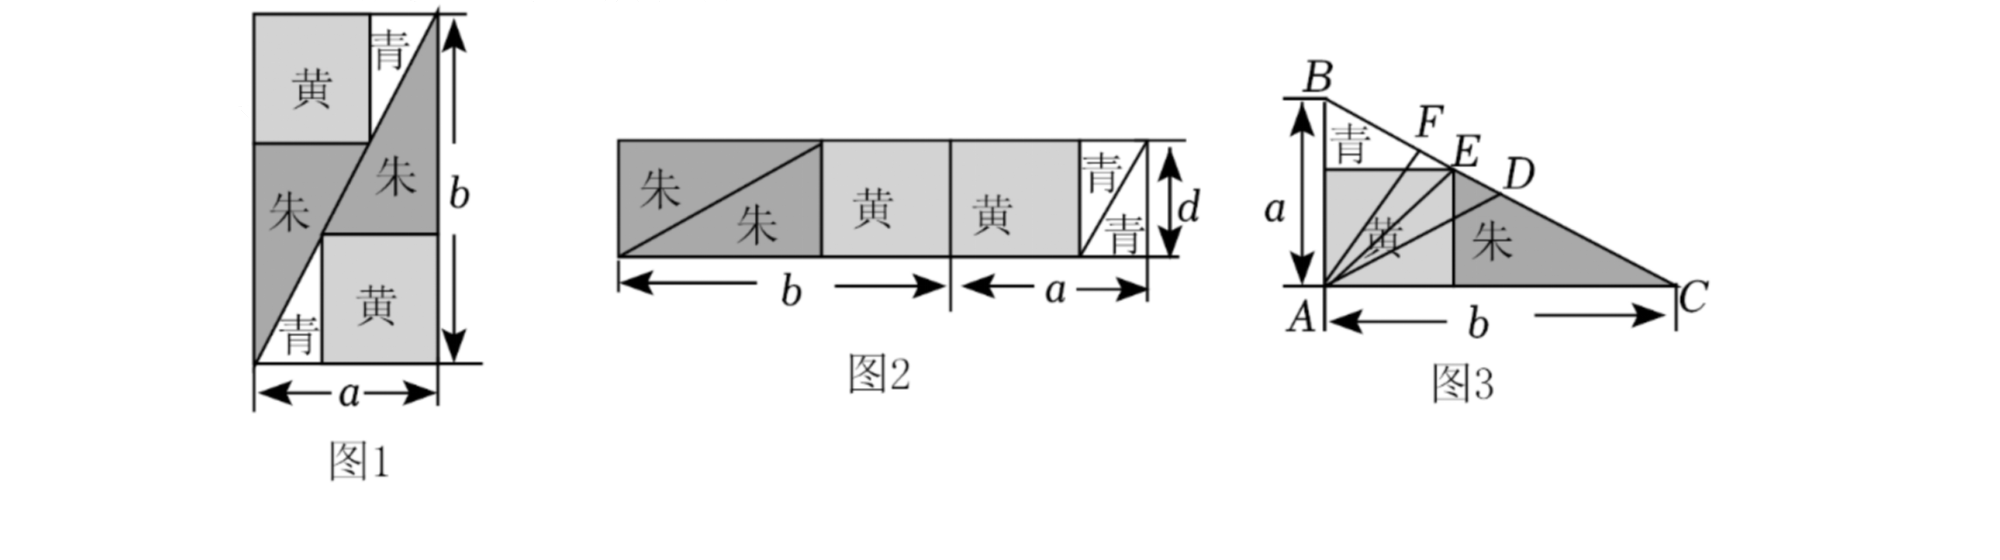
\includegraphics[width=0.86\textwidth]{figures/gao107_q11.png}
\end{center}

①由图 1 和图 2 面积相等得 $d=\dfrac{2ab}{a+b}$　　②由 $AE\geqslant AF$ 可得 $\sqrt{\dfrac{a^2+b^2}2}\geqslant\dfrac{a+b}2$

③由 $AD\geqslant AE$ 可得 $\sqrt{\dfrac{a^2+b^2}2}\geqslant\dfrac{2}{\dfrac1a+\dfrac1b}$　④由 $AD\geqslant AF$ 可得 $a^2+b^2\geqslant2ab$

\ifanswer
\solbegin
\step{对于①，由图 1 和图 2 面积相等得 $ab=(a+b)\times d$，所以 $d=\dfrac{ab}{a+b}$，故①错,}
\step{对于②，因为 $AF\perp BC$，所以 $\dfrac12ab=\dfrac12\sqrt{a^2+b^2}\times AF$,}
\step{所以 $AF=\dfrac{ab}{\sqrt{a^2+b^2}}$，$AE=\sqrt2d=\dfrac{\sqrt2ab}{a+b}$,}
\step{因为 $AE\geqslant AF$，所以 $\dfrac{\sqrt2ab}{a+b}\geqslant\dfrac{ab}{\sqrt{a^2+b^2}}$，整理得 $\sqrt{\dfrac{a^2+b^2}2}\geqslant\dfrac{a+b}2$，故②对,}
\step{对于③，因为 $D$ 是斜边 $BC$ 的中点，所以 $AD=\sqrt{\dfrac{a^2+b^2}2}$,}
\step{因为 $AD\geqslant AE$，所以 $\sqrt{\dfrac{a^2+b^2}2}\geqslant\dfrac{\sqrt2ab}{a+b}$，整理得 $\sqrt{\dfrac{a^2+b^2}2}\geqslant\dfrac{2}{\dfrac1a+\dfrac1b}$，故③对,}
\step{对于④，因为 $AD\geqslant AF$，所以 $\sqrt{\dfrac{a^2+b^2}2}\geqslant\dfrac{ab}{\sqrt{a^2+b^2}}$，整理得 $a^2+b^2\geqslant2ab$,}
\step{故④对,}
\step{故正确的是②③④.}
\solend
\fi

\item 设 $a,b,c,d\in\R$ 且$\lvert a-b\rvert\leqslant2$,$\lvert c-d\rvert\leqslant2$,$\lvert a\rvert\leqslant3$,$\lvert c\rvert\leqslant3$，则 $\lvert ad-bc\rvert$ 的最大值为\blankline[4.4em].% 原卷四处条件间均排半角逗号，照录

\ifanswer
\solbegin
\step{令 $a-b=e$,$c-d=f$，则 $\lvert e\rvert\leqslant2$,$\lvert f\rvert\leqslant2$,$\lvert a\rvert\leqslant3$,$\lvert c\rvert\leqslant3$}
\step{则 $\lvert ad-bc\rvert=\lvert a(c-f)-(a-e)c\rvert=\lvert ce-af\rvert\leqslant\lvert c\rvert\,\lvert e\rvert+\lvert a\rvert\,\lvert f\rvert\leqslant12$,}
\step{则 $\lvert ad-bc\rvert$ 的最大值为 12.}
\solend
\fi

\end{enumerate}

\bigsec{二、选择题}

\begin{enumerate}
\setcounter{enumi}{12}

\item 下列说法正确的是\mbox{（\quad）}

\keepwithprev
A. 若 $a>b>0$，则 $ac^2>bc^2$\qquad\qquad B. 若 $a<b<0$，则 $a^2>ab>b^2$

C. 若 $a>b$，则 $a^2>b^2$\qquad\qquad\qquad D. 若 $a<b$，则 $\dfrac1a>\dfrac1b$

\ifanswer
\solbegin
\step{$A$. 当 $a>b>0$ 时，取 $c=0$，则 $ac^2>bc^2$ 不成立，故 $A$ 错误；}
\step{$B$. 当 $a<b<0$ 时，由不等式的基本性质得 $a^2>ab>b^2>0$，故 $B$ 正确；}
\step{$C$. 当 $a>b$ 时，取 $a=0$，$b=-1$，则 $a^2>b^2$ 不成立，故 $C$ 错误；}
\step{$D$. 当 $a<b$ 时，取 $a=0$，$b=1$，则 $\dfrac1a>\dfrac1b$ 不成立，故 $D$ 错误.}
\step{故选 $B$.}
\solend
\fi

\item 小玲在学习《论语·子路》读到“其身正，不令而行；其身不正，虽令不从”，这句话的
数学含义可以理解为：“身正”是“令行”的\mbox{（\quad）}

\keepwithprev
A. 充分非必要条件\qquad\qquad B. 必要不充分条件

C. 充要条件\qquad\qquad\qquad D. 既非充分又非必要条件

\ifanswer
\solbegin
\step{其身正，不令而行，即身正$\Rightarrow$令行，所以“身正”是“令行”的充分条件；}
\step{又其身不正，虽令不从，即令行$\Rightarrow$身正，所以“身正”是“令行”的必要条件；}
\step{综上，“身正”是“令行”的充要条件. 故选 $C$.}
\solend
\fi

\item 某地对农户抽样调查，结果如下：电冰箱拥有率为 $45\%$，电视机拥有率为 $55\%$，洗衣
机拥有率为 $65\%$，拥有上述三种电器的任意两种的占 $35\%$，三种电器齐全的为 $25\%$，那
么一种电器也没有的农户所占比例是\mbox{（\quad）}

\keepwithprev
A. $12\%$\qquad B. $15\%$\qquad C. $18\%$\qquad D. $20\%$

\ifanswer
\solbegin
\step{设只有电冰箱和电视机的农户有 $a$ 家，只有电冰箱和洗衣机的农户有 $b$ 家,}
\step{只有洗衣机和电视机的农户有 $c$ 家,}
\step{只有电视机、电冰箱、洗衣机的分别有 $d$、$e$、$f$ 家,}
\step{没有任何电器的农户有 $x$ 家,}

\begin{center}
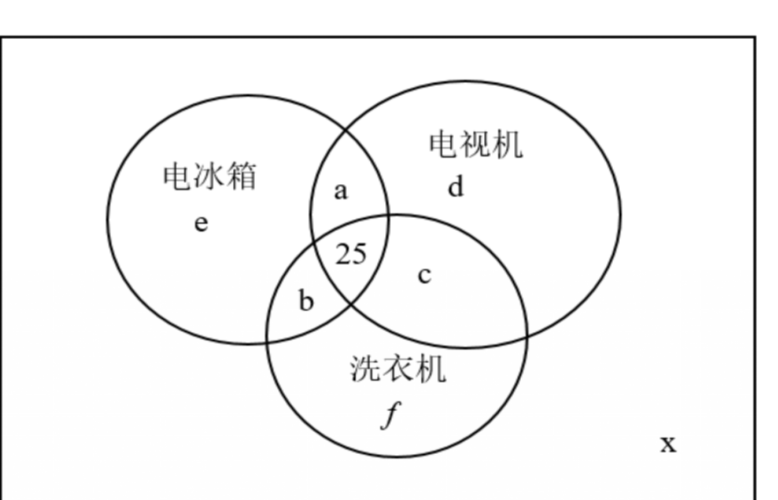
\includegraphics[width=0.42\textwidth]{figures/gao107_q15.png}
\end{center}

\step{所以 $25+a+b+e=45$①，$25+a+c+d=55$②,}
\step{$25+b+c+f=65$③,}
\step{把上面三个式子相加得 $2(a+b+c)+d+e+f=90$④,}
\step{对于拥有上述三种电器的任意两种的占 $35\%$，得 $a+b+c=35$⑤,}
\step{把⑤代入④可得到 $d+e+f=20$⑥,}
\step{因为农户共有 100 家，所以 $25+a+b+c+d+e+f+x=100$,}
\step{把⑤和⑥代入上式得 $x=20$，即一种电器也没有的农户所占比例为 $20\%$.}
\step{故选 $D$.}
\solend
\fi

\item 设 $d>0$，已知 $A,B$ 是两个数集. 若对任意 $x\in A$，都存在 $y\in B$，使得 $\lvert x-y\rvert<d$，则
称 $A$ 是 $B$ 的一个“$d-$邻集”. 现有下列两个命题：① $M=\{a+b\sqrt2\mid a,b\in\Z\}$ 是 $\Q$ 的一个
$\dfrac1{2025}$
一邻集；②若 $A$ 是 $B$ 的一个 $d-$邻集，则 $B$ 也是 $A$ 的一个 $d-$邻集；则\mbox{（\quad）}% 原卷把 d−邻集 的连字符断行后排成“一邻集”，照录

\keepwithprev
A. ①真②假\qquad B. ①假②真\qquad C. ①真②真\qquad D. ①假②假

\ifanswer
\solbegin
\step{对于①，任取 $M$ 中的元素 $x_0=a_0+b_0\sqrt2$,}
\step{则存在 $y_0\in\Q\cap\left(a_0+b_0\sqrt2-\dfrac1{2025},a_0+b_0\sqrt2+\dfrac1{2025}\right)$ 满足题意，故①正确；}
\step{对于②，取 $A=[-1,1]$,$B=[-2,2]$, $A$ 是 $B$ 的 $\dfrac12-$邻集，但反之不成立,}
\step{故②错误；}
\step{故选 $A$.}
\solend
\fi

\end{enumerate}

\bigsec{三、解答题}

\begin{enumerate}
\setcounter{enumi}{16}

\item 设 $a\in\R$，完成下列问题：

（1）求不等式 $3(a+1)x-3>2ax-3a$ 的解集 $M$；

（2）设集合 $A=\{x\mid x^2-ax+a^2-19=0\}$，$B=\{x\mid x^2-5x+6=0\}$，
$C=\{x\mid x^2+2x-8=0\}$. 若 $A\cap B\supset\varnothing$，$A\cap C=\varnothing$，求 $a$ 的值.

\ifanswer
\solbegin
\step{（1）不等式 $3(a+1)x-3>2ax-3a$ 可化为 $(a+3)x>3-3a$,}
\step{当 $a+3>0$，即 $a>-3$ 时，解得 $x>\dfrac{3-3a}{a+3}$,}
\step{当 $a+3=0$，即 $a=-3$ 时，不等式化为 $0\cdot x>12$，无解,}
\step{当 $a+3<0$，即 $a<-3$ 时，解得 $x<\dfrac{3-3a}{a+3}$,}
\step{综上所述，当 $a>-3$ 时，$M=\left(\dfrac{3-3a}{a+3},+\infty\right)$；}
\step{当 $a=-3$ 时，$M=\varnothing$；}
\step{当 $a<-3$ 时，$M=\left(-\infty,\dfrac{3-3a}{a+3}\right)$；}
\step{（2）$B=\{x\mid x^2-5x+6=0\}=\{2,3\}$，$C=\{x\mid x^2+2x-8=0\}=\{2,-4\}$,}
\step{因为 $A\cap B\supset\varnothing$，所以 $A\cap B\neq\varnothing$，又因为 $A\cap C=\varnothing$,}
\step{所以 $3\in A$，$2\notin A$，$-4\notin A$,}
\step{把 $x=3$ 代入方程 $x^2-ax+a^2-19=0$ 得 $9-3a+a^2-19=0$,}
\step{解得 $a=-2$ 或 $a=5$,}
\step{当 $a=-2$ 时，集合 $A=\{x\mid x^2+2x-15=0\}=\{3,-5\}$，符合题意,}
\step{当 $a=5$ 时，集合 $A=\{x\mid x^2-5x+6=0\}=\{3,2\}$，不符合题意，舍去,}
\step{综上所述，$a$ 的值为 $-2$.}
\solend
\fi

\item 完成下列问题：

（1）设 $x$、$y\in\R$，且 $x+y>5$，用反证法证明：$x>3$ 或 $y>2$；

（2）设 $x>0$，$a=x+1$，$b=\sqrt{x^2+7x+1}$，求 $\dfrac ba$ 的最大值.

\ifanswer
\solbegin
\step{（1）假设 $x\leqslant3$ 且 $y\leqslant2$，则 $x+y\leqslant3+2=5$，这与已知 $x+y>5$ 矛盾,}
\step{故 $x>3$ 或 $y>2$；}
\step{（2）$x>0$，$a=x+1$，$b=\sqrt{x^2+7x+1}$,}
\step{则 $\dfrac ba=\dfrac{\sqrt{x^2+7x+1}}{x+1}=\sqrt{\dfrac{x^2+7x+1}{x^2+2x+1}}=\sqrt{\dfrac{x^2+2x+1+5x}{x^2+2x+1}}$}
\step{$=\sqrt{1+\dfrac{5x}{x^2+2x+1}}=\sqrt{1+\dfrac{5}{x+\dfrac1x+2}}\leqslant\sqrt{1+\dfrac{5}{2\sqrt{x\cdot\dfrac1x}+2}}=\dfrac32$,}
\step{当且仅当 $x=\dfrac1x$，即 $x=1$ 时取等号，故 $\dfrac ba$ 的最大值为 $\dfrac32$.}
\solend
\fi

\item 已知函数 $f(x)=\lvert2x-a\rvert+a$.

（1）当 $a=2$ 时，求不等式 $f(x)\leqslant6+\lvert x+2\rvert$ 的解集；

（2）设 $g(x)=\lvert2x-1\rvert$，若不等式 $f(x)+g(x)\geqslant3$ 对一切 $x\in\R$ 恒成立，求实数 $a$ 的取值
范围.

\ifanswer
\solbegin
\ansspace*
\step{（1）$a=2$ 时，$f(x)=\lvert2x-2\rvert+2$,}
\step{则 $f(x)\leqslant6+\lvert x+2\rvert\Leftrightarrow\lvert2x-2\rvert+2\leqslant6+\lvert x+2\rvert$，即 $\lvert2x-2\rvert-\lvert x+2\rvert\leqslant4$,}
\step{当 $x<-2$ 时，$2-2x+x+2\leqslant4$，解得 $x\geqslant0$，与 $x<-2$ 取交集得 $\varnothing$,}
\step{当 $-2\leqslant x\leqslant1$ 时，$2-2x-x-2\leqslant4$，解得 $x\geqslant-\dfrac43$,}
\step{与 $-2\leqslant x\leqslant1$ 取交集得 $-\dfrac43\leqslant x\leqslant1$,}
\step{当 $x>1$ 时，$2x-2-x-2\leqslant4$，解得 $x\leqslant8$，与 $x>1$ 取交集得 $1<x\leqslant8$,}
\step{综上，不等式 $f(x)\leqslant6+\lvert x+2\rvert$ 的解集为 $\left\{x\,\middle|\,-\dfrac43\leqslant x\leqslant8\right\}$；}
\step{（2）$f(x)+g(x)\geqslant3$，即 $\lvert2x-a\rvert+a+\lvert2x-1\rvert\geqslant3$,}
\step{故 $\lvert2x-a\rvert+\lvert2x-1\rvert\geqslant3-a$,}
\step{当 $a\geqslant3$ 时，不等式显然成立,}
\step{当 $a<3$ 时,}
\step{由三角不等式得 $\lvert2x-a\rvert+\lvert2x-1\rvert\geqslant\lvert2x-a-(2x-1)\rvert=\lvert1-a\rvert$,}
\step{当且仅当 $(2x-a)(2x-1)\leqslant0$ 时取等号，因此 $\lvert1-a\rvert\geqslant3-a$,}
\step{平方得 $(1-a)^2\geqslant(3-a)^2$，解得 $a\geqslant2$，故 $2\leqslant a<3$.}
\step{综上，实数 $a$ 的取值范围是 $a\geqslant2$.}
\solend
\fi

\item 对于集合 $A,B$，定义集合 $A-B=\{x\mid x\in A$ 且 $x\notin B\}$.

（1）若 $A=\{1,2,3,4\}$,$B=\{3,4,5\}$，求集合 $A-B$ 和 $B-A$；

（2）给定集合 $A,B$，求所有满足方程组
\[
\begin{cases}
X\cap(A\cup B)=X\\
A\cap(B\cup X)=A\\
B\cap(A\cup X)=B\\
X\cap(A\cap B)=\varnothing
\end{cases}
\]
的集合 $X$（用 $A,B$ 表示）；

（3）用 $\lvert M\rvert$ 表示集合 $M$ 中的元素个数. 给定正整数 $n$，集合 $S=\{1,2,\cdots,n\}$. 对于实数
集的非空有限子集 $A,B$，定义集合 $C=\{x\mid x=a+b,a\in A,b\in B\}$. 求证：

$\lvert A-S\rvert+\lvert B-S\rvert+\lvert S-C\rvert\geqslant1$.

\ifanswer
\solbegin
\step{（1）由 $A=\{1,2,3,4\}$,$B=\{3,4,5\}$，则 $A-B=\{1,2\}$,$B-A=\{5\}$；}
\step{（2）由
$\begin{cases}
X\cap(A\cup B)=X\\
X\cap(A\cap B)=\varnothing
\end{cases}$，
得 $X\subseteq A-B$ 或 $X\subseteq B-A$,}
\step{再结合
$\begin{cases}
A\cap(B\cup X)=A\\
B\cap(A\cup X)=B
\end{cases}$，
得 $X=(A-B)\cup(B-A)$,}
\step{所以 $X=(A-B)\cup(B-A)$；}
\step{（3）$\lvert X\rvert$ 表示集合 $X$ 中的元素个数，则 $\lvert X\rvert\geqslant0$,}
\step{若 $A\cup B$ 中至少含有一个不在 $S$ 中的元素，则 $\lvert A-S\rvert+\lvert B-S\rvert\geqslant1$,}
\step{即 $\lvert A-S\rvert+\lvert B-S\rvert+\lvert S-C\rvert\geqslant1$.}
\step{若 $A\subseteq S$，且 $B\subseteq S$，则 $\lvert A-S\rvert=\lvert B-S\rvert=0$.}
\step{此时 $A$ 中最小的元素 $a\geqslant1$,$B$ 中最小的元素 $b\geqslant1$.}
\step{所以 $C$ 中最小的元素 $a+b\geqslant2$，则 $1\notin C$,}
\step{因为 $S=\{1,2,\cdots,n\}$，所以 $\lvert S-C\rvert\geqslant1$，即 $\lvert A-S\rvert+\lvert B-S\rvert+\lvert S-C\rvert\geqslant1$.}
\step{综上所述，$\lvert A-S\rvert+\lvert B-S\rvert+\lvert S-C\rvert\geqslant1$.}
\solend
\fi

\end{enumerate}

\end{document}
"
%
% 原始材料：微信公众号“魔都数学加油站”文章，作者破晓，2026-11-03 17:19 发布；
% 连载“27学年高一107”，原文标题“27学年高一107——2026-2027年上海市曹杨二中高一上10月月考”；
% 原文链接：https://mp.weixin.qq.com/s/IF4uB7aDNv-snYwbGMoDiQ。
% 正文为 10 张 PNG 页（第 1、2、4、6—9 页 4762×6735，第 3、5、10 页 2560×3620），题目下印有【解析】，为讲评版。
% 题目、解析均据原图转录；卷面水印及公众号页脚未录入。
% 第 11 题题干的三幅“出入相补”图（图 1—图 3）与第 15 题解析的三圆文氏图裁自原图、
% 去粉色水印转灰度（gao107_q11.png、gao107_q15.png），第 11 题图属题干（三版都出）、
% 第 15 题图属解析（仅答案版显示）。
%
% 卷首标题：原卷印作“2026-2027 年曹杨二中高一上 10 月月考”（公众号标题中的“上海市”
% 卷面标题行没有，本稿照卷面），年份区间按全稿惯例排 en dash；原卷未印副标题，本稿按题目内容
% 标为“集合与常用逻辑用语、不等式”。
%
% 与原卷的排版差异：
%   ① 原文从第 3 题起，填空题编号为 3—12、选择题为 13—16、解答题为 17—20，本稿保留原题号；
%   ② 原卷每题下直接印【解析】，本稿按全稿惯例将解析置于答案版；第 4 题只印【答案】另提 \ans{}；
%   ③ 原卷未印副标题，本稿按“知识模块”口径补出；
%   ④ 原卷填空横线按全稿惯例排为 \blankline[4.4em]；解答题按惯例加 \ansspace；选择题括号排
%      \mbox{（\quad）}、选项段前按惯例加 \keepwithprev；
%   ⑤ 原卷数集字母粗体与斜体混用（第 3 题 $\mathbf{R}$、第 4 题斜体 $R$、第 16 题粗体
%      $\mathbf{Z}$、$\mathbf{Q}$ 等），按全稿惯例统一改 \R、\Z、\Q。
%
% 原卷存疑：第 10 题解析“由 $\Delta=16m^2-8(2m^2+3m-2)\geqslant0$ 得 $m\leqslant\dfrac23$”
% 行末原卷无句读，照录。第 16 题解析②“取 $A=[-1,1]$，$B=[-2,2]$，$A$ 是 $B$ 的
% $\dfrac12$-邻集，但反之不成立”，据以判①真②假，照录。
%
% 行数核对：逐题数 \step/\stepm 条数，合计 112 条（Q3：5；Q4：0；Q5：2；Q6：2；Q7：2；
% Q8：4；Q9：8；Q10：4；Q11：9；Q12：3；Q13：5；Q14：3；Q15：12；Q16：5；Q17：15；
% Q18：6；Q19：15；Q20：12），与原卷印刷行逐题相等。第 4 题只印【答案】，提 \ans{}，
% 不计入 \step 账。
%
\documentclass[a4paper,11pt]{article}
\usepackage{common}

\begin{document}

\examtitlest[3]{2026--2027 年曹杨二中高一上 10 月月考}{集合与常用逻辑用语、不等式}

\bigsec{一、填空题}

\begin{enumerate}
\setcounter{enumi}{2}

\item 设 $a\in\R$，若 $3\in\{\sqrt3,a^2,a\}$，则 $a=$\blankline[4.4em].

\ifanswer
\solbegin
\step{因为 $3\in\{\sqrt3,a^2,a\}$，所以 $a^2=3$，解得 $a=\sqrt3$ 或 $a=-\sqrt3$,}
\step{当 $a=\sqrt3$ 时，集合为 $\{\sqrt3,3,\sqrt3\}$，不满足集合元素的互异性，舍去；}
\step{当 $a=-\sqrt3$ 时，集合为 $\{\sqrt3,3,-\sqrt3\}$，符合要求；}
\step{若 $a=3$，此时集合为 $\{\sqrt3,9,3\}$，符合要求；}
\step{综上，$a$ 为 $-\sqrt3$ 或 $3$.}
\solend
\fi

\item 设 $a\in\R$，已知集合 $A=\{x\mid x\leqslant a\}$，$B=\{x\mid x>2\}$. 若 $A\cup B=\R$，则 $a$ 的取值范围是\blankline[4.4em].

\ifanswer
\ans{$a\geqslant2$}
\fi

\item 设 $x>0$，$y>0$ 且 $x+3y=1$，则 $xy$ 的最大值为\blankline[4.4em].

\ifanswer
\solbegin
\step{由于 $x>0$，$y>0$ 且 $x+3y=1$，则 $1=x+3y\geqslant2\sqrt{3xy}$，得 $xy\leqslant\dfrac1{12}$,}
\step{当且仅当 $x=3y=\dfrac12$ 时取等号，则 $xy$ 的最大值为 $\dfrac1{12}$.}
\solend
\fi

\item 设 $a\in\R$，若集合$\left\{x\,\middle|\,\dfrac{ax}{x-1}=x\right\}$有且仅有两个子集，则 $a=$\blankline[4.4em].

\ifanswer
\solbegin
\step{由 $\dfrac{ax}{x-1}=x$ 得 $ax=x(x-1)$，即 $x(x-a-1)=0$,}
\step{所以此方程有两个相等的（不等于 1）的实数根或有一根为 1，所以 $a=-1$ 或 $0$.}
\solend
\fi

\item 已知全集 $U=\{x\mid x^2-8x-20<0\}$，集合 $A=\{x\mid 1-x^2>0$ 且 $x<0\}$，则 $\overline A=$\blankline[4.4em].

\ifanswer
\solbegin
\step{$U=\{x\mid-2<x<10\}$，$A=\{x\mid-1<x<0\}$,}
\step{所以 $\overline A=\{x\mid-2<x\leqslant-1$ 或 $0\leqslant x<10\}$.}
\solend
\fi

\item 设 $a,b\in\R$，若不等式 $-x^2-ax+b\geqslant0$ 的解集为 $[-2,3]$，则不等式 $\lvert ax+b\rvert<5$ 的解集为\blankline[4.4em].

\ifanswer
\solbegin
\step{由不等式 $-x^2-ax+b\geqslant0$ 的解集为 $[-2,3]$,}
\step{得 $-2$、$3$ 是方程 $-x^2-ax+b=0$ 的两个根，所以 $a=-1$，$b=6$.}
\step{解不等式 $\lvert-x+6\rvert<5$，得 $-5<x-6<5$，解得 $1<x<11$,}
\step{即所求不等式的解集为 $(1,11)$.}
\solend
\fi

\item 某货运卡车以 $x$ 千米／时的速度匀速行驶 300 千米，按交通法规限制 $50\leqslant x\leqslant100$，假设
柴油的价格为每升 6 元，汽车每小时耗油 $\left(4+\dfrac{x^2}{420}\right)$ 升，司机工资为每小时 46 元. 则当
$x=$\blankline[4.4em]（千米／时），这次行车的总费用（油费与司机工资的总和）最低.

\ifanswer
\solbegin
\step{因为卡车行驶 300 千米，速度为 $x$ 千米／时,}
\step{因此总用时为 $t=\dfrac{300}{x}$ 小时，其中 $50\leqslant x\leqslant100$,}
\step{每小时油费为 $6\cdot\left(4+\dfrac{x^2}{420}\right)$ 元，每小时司机工资为 46 元，因}
\step{此每小时总支出为 $6\cdot\left(4+\dfrac{x^2}{420}\right)+46=70+\dfrac{x^2}{70}$ 元.}
\step{设全程总费用为 $y$，则 $y=\dfrac{300}{x}\cdot\left(70+\dfrac{x^2}{70}\right)=\dfrac{21000}{x}+\dfrac{30x}{7}$,}
\step{因为 $50\leqslant x\leqslant100$，$\dfrac{21000}{x}+\dfrac{30x}{7}\geqslant2\sqrt{\dfrac{21000}{x}\cdot\dfrac{30x}{7}}=600$,}
\step{当且仅当 $\dfrac{21000}{x}=\dfrac{30x}{7}$，即 $x=70$ 时取等号，且 $70\in[50,100]$,}
\step{因此当 $x=70$ 千米／时，行车的总费用（油费与司机工资的总和）最低.}
\solend
\fi

\item 设 $x_1$、$x_2$ 是关于 $x$ 的方程 $2x^2-4mx+2m^2+3m-2=0$ 的两个实数根，则 $x_1^2+x_2^2$ 的最小值为\blankline[4.4em].

\ifanswer
\solbegin
\step{由题意得 $x_1+x_2=2m$，$x_1x_2=m^2+\dfrac{3m}{2}-1$,}
\step{由 $\Delta=16m^2-8(2m^2+3m-2)\geqslant0$ 得 $m\leqslant\dfrac23$}
\step{所以 $x_1^2+x_1^2=(x_1+x_2)^2-2x_1x_2=4m^2-2m^2+3m+2=2m^2-3m+2$,% 原卷左端作 x_1²+x_1²，照录
}
\step{结合二次函数的性质得，当 $m=\dfrac23$ 时取得最小值 $\dfrac89$.}
\solend
\fi

\item 小玲在钻研《九章算术》中“勾股容方”问题“今有勾五步，股十二步，问勾中容方几
何？”时，发现魏晋时期数学家刘徽在其《九章算术注》中利用出入相补原理给出了这个
问题的一般解法：如图 1，用对角线将长和宽分别为 $b$ 和 $a$ 的矩形分成两个直角三角形，
每个直角三角形再分成一个内接正方形（黄）和两个小直角三角形（朱、青）. 将三种颜色
的图形进行重组，得到如图 2 所示的矩形，该矩形长为 $a+b$，宽为内接正方形的边长
$d$. 由刘徽构造的图形可以得到许多重要的结论，如图 3，设 $D$ 为斜边 $BC$ 的中点，作直
角三角形 $ABC$ 的内接正方形对角线 $AE$，过点 $A$ 作 $AF\perp BC$ 于点 $F$，则下列四个推理中
正确的序号是\blankline[4.4em].

\begin{center}
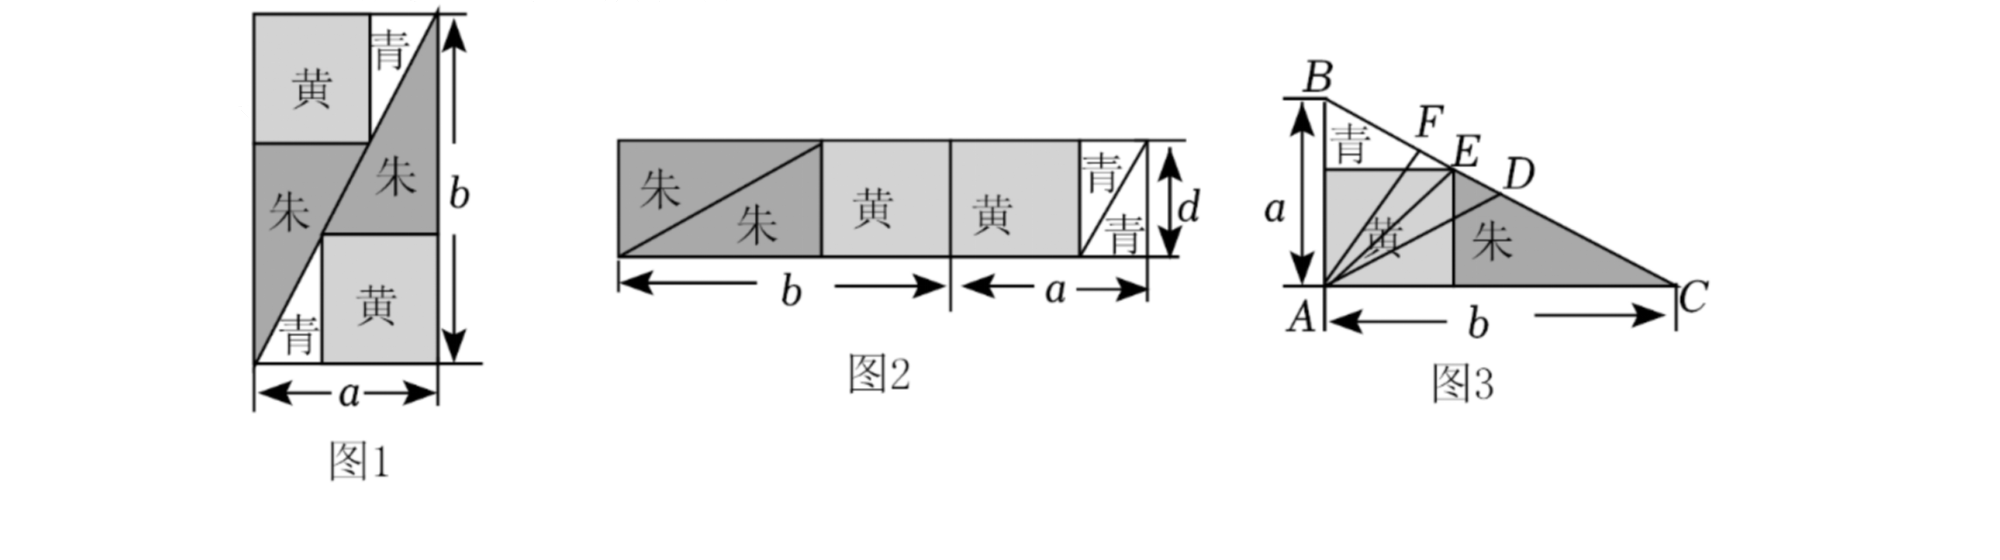
\includegraphics[width=0.86\textwidth]{figures/gao107_q11.png}
\end{center}

①由图 1 和图 2 面积相等得 $d=\dfrac{2ab}{a+b}$　　②由 $AE\geqslant AF$ 可得 $\sqrt{\dfrac{a^2+b^2}2}\geqslant\dfrac{a+b}2$

③由 $AD\geqslant AE$ 可得 $\sqrt{\dfrac{a^2+b^2}2}\geqslant\dfrac{2}{\dfrac1a+\dfrac1b}$　④由 $AD\geqslant AF$ 可得 $a^2+b^2\geqslant2ab$

\ifanswer
\solbegin
\step{对于①，由图 1 和图 2 面积相等得 $ab=(a+b)\times d$，所以 $d=\dfrac{ab}{a+b}$，故①错,}
\step{对于②，因为 $AF\perp BC$，所以 $\dfrac12ab=\dfrac12\sqrt{a^2+b^2}\times AF$,}
\step{所以 $AF=\dfrac{ab}{\sqrt{a^2+b^2}}$，$AE=\sqrt2d=\dfrac{\sqrt2ab}{a+b}$,}
\step{因为 $AE\geqslant AF$，所以 $\dfrac{\sqrt2ab}{a+b}\geqslant\dfrac{ab}{\sqrt{a^2+b^2}}$，整理得 $\sqrt{\dfrac{a^2+b^2}2}\geqslant\dfrac{a+b}2$，故②对,}
\step{对于③，因为 $D$ 是斜边 $BC$ 的中点，所以 $AD=\sqrt{\dfrac{a^2+b^2}2}$,}
\step{因为 $AD\geqslant AE$，所以 $\sqrt{\dfrac{a^2+b^2}2}\geqslant\dfrac{\sqrt2ab}{a+b}$，整理得 $\sqrt{\dfrac{a^2+b^2}2}\geqslant\dfrac{2}{\dfrac1a+\dfrac1b}$，故③对,}
\step{对于④，因为 $AD\geqslant AF$，所以 $\sqrt{\dfrac{a^2+b^2}2}\geqslant\dfrac{ab}{\sqrt{a^2+b^2}}$，整理得 $a^2+b^2\geqslant2ab$,}
\step{故④对,}
\step{故正确的是②③④.}
\solend
\fi

\item 设 $a,b,c,d\in\R$ 且$\lvert a-b\rvert\leqslant2$,$\lvert c-d\rvert\leqslant2$,$\lvert a\rvert\leqslant3$,$\lvert c\rvert\leqslant3$，则 $\lvert ad-bc\rvert$ 的最大值为\blankline[4.4em].% 原卷四处条件间均排半角逗号，照录

\ifanswer
\solbegin
\step{令 $a-b=e$,$c-d=f$，则 $\lvert e\rvert\leqslant2$,$\lvert f\rvert\leqslant2$,$\lvert a\rvert\leqslant3$,$\lvert c\rvert\leqslant3$}
\step{则 $\lvert ad-bc\rvert=\lvert a(c-f)-(a-e)c\rvert=\lvert ce-af\rvert\leqslant\lvert c\rvert\,\lvert e\rvert+\lvert a\rvert\,\lvert f\rvert\leqslant12$,}
\step{则 $\lvert ad-bc\rvert$ 的最大值为 12.}
\solend
\fi

\end{enumerate}

\bigsec{二、选择题}

\begin{enumerate}
\setcounter{enumi}{12}

\item 下列说法正确的是\mbox{（\quad）}

\keepwithprev
A. 若 $a>b>0$，则 $ac^2>bc^2$\qquad\qquad B. 若 $a<b<0$，则 $a^2>ab>b^2$

C. 若 $a>b$，则 $a^2>b^2$\qquad\qquad\qquad D. 若 $a<b$，则 $\dfrac1a>\dfrac1b$

\ifanswer
\solbegin
\step{$A$. 当 $a>b>0$ 时，取 $c=0$，则 $ac^2>bc^2$ 不成立，故 $A$ 错误；}
\step{$B$. 当 $a<b<0$ 时，由不等式的基本性质得 $a^2>ab>b^2>0$，故 $B$ 正确；}
\step{$C$. 当 $a>b$ 时，取 $a=0$，$b=-1$，则 $a^2>b^2$ 不成立，故 $C$ 错误；}
\step{$D$. 当 $a<b$ 时，取 $a=0$，$b=1$，则 $\dfrac1a>\dfrac1b$ 不成立，故 $D$ 错误.}
\step{故选 $B$.}
\solend
\fi

\item 小玲在学习《论语·子路》读到“其身正，不令而行；其身不正，虽令不从”，这句话的
数学含义可以理解为：“身正”是“令行”的\mbox{（\quad）}

\keepwithprev
A. 充分非必要条件\qquad\qquad B. 必要不充分条件

C. 充要条件\qquad\qquad\qquad D. 既非充分又非必要条件

\ifanswer
\solbegin
\step{其身正，不令而行，即身正$\Rightarrow$令行，所以“身正”是“令行”的充分条件；}
\step{又其身不正，虽令不从，即令行$\Rightarrow$身正，所以“身正”是“令行”的必要条件；}
\step{综上，“身正”是“令行”的充要条件. 故选 $C$.}
\solend
\fi

\item 某地对农户抽样调查，结果如下：电冰箱拥有率为 $45\%$，电视机拥有率为 $55\%$，洗衣
机拥有率为 $65\%$，拥有上述三种电器的任意两种的占 $35\%$，三种电器齐全的为 $25\%$，那
么一种电器也没有的农户所占比例是\mbox{（\quad）}

\keepwithprev
A. $12\%$\qquad B. $15\%$\qquad C. $18\%$\qquad D. $20\%$

\ifanswer
\solbegin
\step{设只有电冰箱和电视机的农户有 $a$ 家，只有电冰箱和洗衣机的农户有 $b$ 家,}
\step{只有洗衣机和电视机的农户有 $c$ 家,}
\step{只有电视机、电冰箱、洗衣机的分别有 $d$、$e$、$f$ 家,}
\step{没有任何电器的农户有 $x$ 家,}

\begin{center}
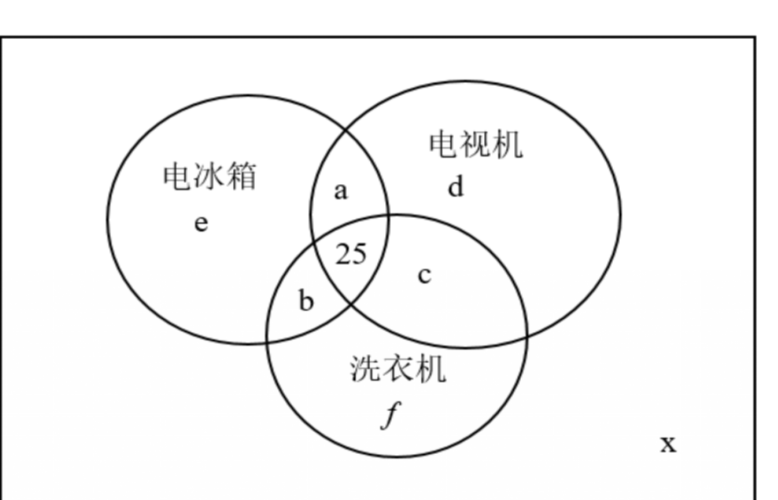
\includegraphics[width=0.42\textwidth]{figures/gao107_q15.png}
\end{center}

\step{所以 $25+a+b+e=45$①，$25+a+c+d=55$②,}
\step{$25+b+c+f=65$③,}
\step{把上面三个式子相加得 $2(a+b+c)+d+e+f=90$④,}
\step{对于拥有上述三种电器的任意两种的占 $35\%$，得 $a+b+c=35$⑤,}
\step{把⑤代入④可得到 $d+e+f=20$⑥,}
\step{因为农户共有 100 家，所以 $25+a+b+c+d+e+f+x=100$,}
\step{把⑤和⑥代入上式得 $x=20$，即一种电器也没有的农户所占比例为 $20\%$.}
\step{故选 $D$.}
\solend
\fi

\item 设 $d>0$，已知 $A,B$ 是两个数集. 若对任意 $x\in A$，都存在 $y\in B$，使得 $\lvert x-y\rvert<d$，则
称 $A$ 是 $B$ 的一个“$d-$邻集”. 现有下列两个命题：① $M=\{a+b\sqrt2\mid a,b\in\Z\}$ 是 $\Q$ 的一个
$\dfrac1{2025}$
一邻集；②若 $A$ 是 $B$ 的一个 $d-$邻集，则 $B$ 也是 $A$ 的一个 $d-$邻集；则\mbox{（\quad）}% 原卷把 d−邻集 的连字符断行后排成“一邻集”，照录

\keepwithprev
A. ①真②假\qquad B. ①假②真\qquad C. ①真②真\qquad D. ①假②假

\ifanswer
\solbegin
\step{对于①，任取 $M$ 中的元素 $x_0=a_0+b_0\sqrt2$,}
\step{则存在 $y_0\in\Q\cap\left(a_0+b_0\sqrt2-\dfrac1{2025},a_0+b_0\sqrt2+\dfrac1{2025}\right)$ 满足题意，故①正确；}
\step{对于②，取 $A=[-1,1]$,$B=[-2,2]$, $A$ 是 $B$ 的 $\dfrac12-$邻集，但反之不成立,}
\step{故②错误；}
\step{故选 $A$.}
\solend
\fi

\end{enumerate}

\bigsec{三、解答题}

\begin{enumerate}
\setcounter{enumi}{16}

\item 设 $a\in\R$，完成下列问题：

（1）求不等式 $3(a+1)x-3>2ax-3a$ 的解集 $M$；

（2）设集合 $A=\{x\mid x^2-ax+a^2-19=0\}$，$B=\{x\mid x^2-5x+6=0\}$，
$C=\{x\mid x^2+2x-8=0\}$. 若 $A\cap B\supset\varnothing$，$A\cap C=\varnothing$，求 $a$ 的值.

\ifanswer
\solbegin
\step{（1）不等式 $3(a+1)x-3>2ax-3a$ 可化为 $(a+3)x>3-3a$,}
\step{当 $a+3>0$，即 $a>-3$ 时，解得 $x>\dfrac{3-3a}{a+3}$,}
\step{当 $a+3=0$，即 $a=-3$ 时，不等式化为 $0\cdot x>12$，无解,}
\step{当 $a+3<0$，即 $a<-3$ 时，解得 $x<\dfrac{3-3a}{a+3}$,}
\step{综上所述，当 $a>-3$ 时，$M=\left(\dfrac{3-3a}{a+3},+\infty\right)$；}
\step{当 $a=-3$ 时，$M=\varnothing$；}
\step{当 $a<-3$ 时，$M=\left(-\infty,\dfrac{3-3a}{a+3}\right)$；}
\step{（2）$B=\{x\mid x^2-5x+6=0\}=\{2,3\}$，$C=\{x\mid x^2+2x-8=0\}=\{2,-4\}$,}
\step{因为 $A\cap B\supset\varnothing$，所以 $A\cap B\neq\varnothing$，又因为 $A\cap C=\varnothing$,}
\step{所以 $3\in A$，$2\notin A$，$-4\notin A$,}
\step{把 $x=3$ 代入方程 $x^2-ax+a^2-19=0$ 得 $9-3a+a^2-19=0$,}
\step{解得 $a=-2$ 或 $a=5$,}
\step{当 $a=-2$ 时，集合 $A=\{x\mid x^2+2x-15=0\}=\{3,-5\}$，符合题意,}
\step{当 $a=5$ 时，集合 $A=\{x\mid x^2-5x+6=0\}=\{3,2\}$，不符合题意，舍去,}
\step{综上所述，$a$ 的值为 $-2$.}
\solend
\fi

\item 完成下列问题：

（1）设 $x$、$y\in\R$，且 $x+y>5$，用反证法证明：$x>3$ 或 $y>2$；

（2）设 $x>0$，$a=x+1$，$b=\sqrt{x^2+7x+1}$，求 $\dfrac ba$ 的最大值.

\ifanswer
\solbegin
\step{（1）假设 $x\leqslant3$ 且 $y\leqslant2$，则 $x+y\leqslant3+2=5$，这与已知 $x+y>5$ 矛盾,}
\step{故 $x>3$ 或 $y>2$；}
\step{（2）$x>0$，$a=x+1$，$b=\sqrt{x^2+7x+1}$,}
\step{则 $\dfrac ba=\dfrac{\sqrt{x^2+7x+1}}{x+1}=\sqrt{\dfrac{x^2+7x+1}{x^2+2x+1}}=\sqrt{\dfrac{x^2+2x+1+5x}{x^2+2x+1}}$}
\step{$=\sqrt{1+\dfrac{5x}{x^2+2x+1}}=\sqrt{1+\dfrac{5}{x+\dfrac1x+2}}\leqslant\sqrt{1+\dfrac{5}{2\sqrt{x\cdot\dfrac1x}+2}}=\dfrac32$,}
\step{当且仅当 $x=\dfrac1x$，即 $x=1$ 时取等号，故 $\dfrac ba$ 的最大值为 $\dfrac32$.}
\solend
\fi

\item 已知函数 $f(x)=\lvert2x-a\rvert+a$.

（1）当 $a=2$ 时，求不等式 $f(x)\leqslant6+\lvert x+2\rvert$ 的解集；

（2）设 $g(x)=\lvert2x-1\rvert$，若不等式 $f(x)+g(x)\geqslant3$ 对一切 $x\in\R$ 恒成立，求实数 $a$ 的取值
范围.

\ifanswer
\solbegin
\ansspace*
\step{（1）$a=2$ 时，$f(x)=\lvert2x-2\rvert+2$,}
\step{则 $f(x)\leqslant6+\lvert x+2\rvert\Leftrightarrow\lvert2x-2\rvert+2\leqslant6+\lvert x+2\rvert$，即 $\lvert2x-2\rvert-\lvert x+2\rvert\leqslant4$,}
\step{当 $x<-2$ 时，$2-2x+x+2\leqslant4$，解得 $x\geqslant0$，与 $x<-2$ 取交集得 $\varnothing$,}
\step{当 $-2\leqslant x\leqslant1$ 时，$2-2x-x-2\leqslant4$，解得 $x\geqslant-\dfrac43$,}
\step{与 $-2\leqslant x\leqslant1$ 取交集得 $-\dfrac43\leqslant x\leqslant1$,}
\step{当 $x>1$ 时，$2x-2-x-2\leqslant4$，解得 $x\leqslant8$，与 $x>1$ 取交集得 $1<x\leqslant8$,}
\step{综上，不等式 $f(x)\leqslant6+\lvert x+2\rvert$ 的解集为 $\left\{x\,\middle|\,-\dfrac43\leqslant x\leqslant8\right\}$；}
\step{（2）$f(x)+g(x)\geqslant3$，即 $\lvert2x-a\rvert+a+\lvert2x-1\rvert\geqslant3$,}
\step{故 $\lvert2x-a\rvert+\lvert2x-1\rvert\geqslant3-a$,}
\step{当 $a\geqslant3$ 时，不等式显然成立,}
\step{当 $a<3$ 时,}
\step{由三角不等式得 $\lvert2x-a\rvert+\lvert2x-1\rvert\geqslant\lvert2x-a-(2x-1)\rvert=\lvert1-a\rvert$,}
\step{当且仅当 $(2x-a)(2x-1)\leqslant0$ 时取等号，因此 $\lvert1-a\rvert\geqslant3-a$,}
\step{平方得 $(1-a)^2\geqslant(3-a)^2$，解得 $a\geqslant2$，故 $2\leqslant a<3$.}
\step{综上，实数 $a$ 的取值范围是 $a\geqslant2$.}
\solend
\fi

\item 对于集合 $A,B$，定义集合 $A-B=\{x\mid x\in A$ 且 $x\notin B\}$.

（1）若 $A=\{1,2,3,4\}$,$B=\{3,4,5\}$，求集合 $A-B$ 和 $B-A$；

（2）给定集合 $A,B$，求所有满足方程组
\[
\begin{cases}
X\cap(A\cup B)=X\\
A\cap(B\cup X)=A\\
B\cap(A\cup X)=B\\
X\cap(A\cap B)=\varnothing
\end{cases}
\]
的集合 $X$（用 $A,B$ 表示）；

（3）用 $\lvert M\rvert$ 表示集合 $M$ 中的元素个数. 给定正整数 $n$，集合 $S=\{1,2,\cdots,n\}$. 对于实数
集的非空有限子集 $A,B$，定义集合 $C=\{x\mid x=a+b,a\in A,b\in B\}$. 求证：

$\lvert A-S\rvert+\lvert B-S\rvert+\lvert S-C\rvert\geqslant1$.

\ifanswer
\solbegin
\step{（1）由 $A=\{1,2,3,4\}$,$B=\{3,4,5\}$，则 $A-B=\{1,2\}$,$B-A=\{5\}$；}
\step{（2）由
$\begin{cases}
X\cap(A\cup B)=X\\
X\cap(A\cap B)=\varnothing
\end{cases}$，
得 $X\subseteq A-B$ 或 $X\subseteq B-A$,}
\step{再结合
$\begin{cases}
A\cap(B\cup X)=A\\
B\cap(A\cup X)=B
\end{cases}$，
得 $X=(A-B)\cup(B-A)$,}
\step{所以 $X=(A-B)\cup(B-A)$；}
\step{（3）$\lvert X\rvert$ 表示集合 $X$ 中的元素个数，则 $\lvert X\rvert\geqslant0$,}
\step{若 $A\cup B$ 中至少含有一个不在 $S$ 中的元素，则 $\lvert A-S\rvert+\lvert B-S\rvert\geqslant1$,}
\step{即 $\lvert A-S\rvert+\lvert B-S\rvert+\lvert S-C\rvert\geqslant1$.}
\step{若 $A\subseteq S$，且 $B\subseteq S$，则 $\lvert A-S\rvert=\lvert B-S\rvert=0$.}
\step{此时 $A$ 中最小的元素 $a\geqslant1$,$B$ 中最小的元素 $b\geqslant1$.}
\step{所以 $C$ 中最小的元素 $a+b\geqslant2$，则 $1\notin C$,}
\step{因为 $S=\{1,2,\cdots,n\}$，所以 $\lvert S-C\rvert\geqslant1$，即 $\lvert A-S\rvert+\lvert B-S\rvert+\lvert S-C\rvert\geqslant1$.}
\step{综上所述，$\lvert A-S\rvert+\lvert B-S\rvert+\lvert S-C\rvert\geqslant1$.}
\solend
\fi

\end{enumerate}

\end{document}
"
% 紧凑版：xelatex "\def\iscompact{1}% 高一107_曹杨二中_10月月考.tex
%   —— 高一上数学“2026-2027 年曹杨二中高一上 10 月月考”（试卷版/答案版）
% 试卷版：xelatex 高一107_曹杨二中_10月月考.tex
% 答案版：xelatex "\def\isanswer{1}% 高一107_曹杨二中_10月月考.tex
%   —— 高一上数学“2026-2027 年曹杨二中高一上 10 月月考”（试卷版/答案版）
% 试卷版：xelatex 高一107_曹杨二中_10月月考.tex
% 答案版：xelatex "\def\isanswer{1}\input{高一107_曹杨二中_10月月考.tex}"
% 紧凑版：xelatex "\def\iscompact{1}\input{高一107_曹杨二中_10月月考.tex}"
%
% 原始材料：微信公众号“魔都数学加油站”文章，作者破晓，2026-11-03 17:19 发布；
% 连载“27学年高一107”，原文标题“27学年高一107——2026-2027年上海市曹杨二中高一上10月月考”；
% 原文链接：https://mp.weixin.qq.com/s/IF4uB7aDNv-snYwbGMoDiQ。
% 正文为 10 张 PNG 页（第 1、2、4、6—9 页 4762×6735，第 3、5、10 页 2560×3620），题目下印有【解析】，为讲评版。
% 题目、解析均据原图转录；卷面水印及公众号页脚未录入。
% 第 11 题题干的三幅“出入相补”图（图 1—图 3）与第 15 题解析的三圆文氏图裁自原图、
% 去粉色水印转灰度（gao107_q11.png、gao107_q15.png），第 11 题图属题干（三版都出）、
% 第 15 题图属解析（仅答案版显示）。
%
% 卷首标题：原卷印作“2026-2027 年曹杨二中高一上 10 月月考”（公众号标题中的“上海市”
% 卷面标题行没有，本稿照卷面），年份区间按全稿惯例排 en dash；原卷未印副标题，本稿按题目内容
% 标为“集合与常用逻辑用语、不等式”。
%
% 与原卷的排版差异：
%   ① 原文从第 3 题起，填空题编号为 3—12、选择题为 13—16、解答题为 17—20，本稿保留原题号；
%   ② 原卷每题下直接印【解析】，本稿按全稿惯例将解析置于答案版；第 4 题只印【答案】另提 \ans{}；
%   ③ 原卷未印副标题，本稿按“知识模块”口径补出；
%   ④ 原卷填空横线按全稿惯例排为 \blankline[4.4em]；解答题按惯例加 \ansspace；选择题括号排
%      \mbox{（\quad）}、选项段前按惯例加 \keepwithprev；
%   ⑤ 原卷数集字母粗体与斜体混用（第 3 题 $\mathbf{R}$、第 4 题斜体 $R$、第 16 题粗体
%      $\mathbf{Z}$、$\mathbf{Q}$ 等），按全稿惯例统一改 \R、\Z、\Q。
%
% 原卷存疑：第 10 题解析“由 $\Delta=16m^2-8(2m^2+3m-2)\geqslant0$ 得 $m\leqslant\dfrac23$”
% 行末原卷无句读，照录。第 16 题解析②“取 $A=[-1,1]$，$B=[-2,2]$，$A$ 是 $B$ 的
% $\dfrac12$-邻集，但反之不成立”，据以判①真②假，照录。
%
% 行数核对：逐题数 \step/\stepm 条数，合计 112 条（Q3：5；Q4：0；Q5：2；Q6：2；Q7：2；
% Q8：4；Q9：8；Q10：4；Q11：9；Q12：3；Q13：5；Q14：3；Q15：12；Q16：5；Q17：15；
% Q18：6；Q19：15；Q20：12），与原卷印刷行逐题相等。第 4 题只印【答案】，提 \ans{}，
% 不计入 \step 账。
%
\documentclass[a4paper,11pt]{article}
\usepackage{common}

\begin{document}

\examtitlest[3]{2026--2027 年曹杨二中高一上 10 月月考}{集合与常用逻辑用语、不等式}

\bigsec{一、填空题}

\begin{enumerate}
\setcounter{enumi}{2}

\item 设 $a\in\R$，若 $3\in\{\sqrt3,a^2,a\}$，则 $a=$\blankline[4.4em].

\ifanswer
\solbegin
\step{因为 $3\in\{\sqrt3,a^2,a\}$，所以 $a^2=3$，解得 $a=\sqrt3$ 或 $a=-\sqrt3$,}
\step{当 $a=\sqrt3$ 时，集合为 $\{\sqrt3,3,\sqrt3\}$，不满足集合元素的互异性，舍去；}
\step{当 $a=-\sqrt3$ 时，集合为 $\{\sqrt3,3,-\sqrt3\}$，符合要求；}
\step{若 $a=3$，此时集合为 $\{\sqrt3,9,3\}$，符合要求；}
\step{综上，$a$ 为 $-\sqrt3$ 或 $3$.}
\solend
\fi

\item 设 $a\in\R$，已知集合 $A=\{x\mid x\leqslant a\}$，$B=\{x\mid x>2\}$. 若 $A\cup B=\R$，则 $a$ 的取值范围是\blankline[4.4em].

\ifanswer
\ans{$a\geqslant2$}
\fi

\item 设 $x>0$，$y>0$ 且 $x+3y=1$，则 $xy$ 的最大值为\blankline[4.4em].

\ifanswer
\solbegin
\step{由于 $x>0$，$y>0$ 且 $x+3y=1$，则 $1=x+3y\geqslant2\sqrt{3xy}$，得 $xy\leqslant\dfrac1{12}$,}
\step{当且仅当 $x=3y=\dfrac12$ 时取等号，则 $xy$ 的最大值为 $\dfrac1{12}$.}
\solend
\fi

\item 设 $a\in\R$，若集合$\left\{x\,\middle|\,\dfrac{ax}{x-1}=x\right\}$有且仅有两个子集，则 $a=$\blankline[4.4em].

\ifanswer
\solbegin
\step{由 $\dfrac{ax}{x-1}=x$ 得 $ax=x(x-1)$，即 $x(x-a-1)=0$,}
\step{所以此方程有两个相等的（不等于 1）的实数根或有一根为 1，所以 $a=-1$ 或 $0$.}
\solend
\fi

\item 已知全集 $U=\{x\mid x^2-8x-20<0\}$，集合 $A=\{x\mid 1-x^2>0$ 且 $x<0\}$，则 $\overline A=$\blankline[4.4em].

\ifanswer
\solbegin
\step{$U=\{x\mid-2<x<10\}$，$A=\{x\mid-1<x<0\}$,}
\step{所以 $\overline A=\{x\mid-2<x\leqslant-1$ 或 $0\leqslant x<10\}$.}
\solend
\fi

\item 设 $a,b\in\R$，若不等式 $-x^2-ax+b\geqslant0$ 的解集为 $[-2,3]$，则不等式 $\lvert ax+b\rvert<5$ 的解集为\blankline[4.4em].

\ifanswer
\solbegin
\step{由不等式 $-x^2-ax+b\geqslant0$ 的解集为 $[-2,3]$,}
\step{得 $-2$、$3$ 是方程 $-x^2-ax+b=0$ 的两个根，所以 $a=-1$，$b=6$.}
\step{解不等式 $\lvert-x+6\rvert<5$，得 $-5<x-6<5$，解得 $1<x<11$,}
\step{即所求不等式的解集为 $(1,11)$.}
\solend
\fi

\item 某货运卡车以 $x$ 千米／时的速度匀速行驶 300 千米，按交通法规限制 $50\leqslant x\leqslant100$，假设
柴油的价格为每升 6 元，汽车每小时耗油 $\left(4+\dfrac{x^2}{420}\right)$ 升，司机工资为每小时 46 元. 则当
$x=$\blankline[4.4em]（千米／时），这次行车的总费用（油费与司机工资的总和）最低.

\ifanswer
\solbegin
\step{因为卡车行驶 300 千米，速度为 $x$ 千米／时,}
\step{因此总用时为 $t=\dfrac{300}{x}$ 小时，其中 $50\leqslant x\leqslant100$,}
\step{每小时油费为 $6\cdot\left(4+\dfrac{x^2}{420}\right)$ 元，每小时司机工资为 46 元，因}
\step{此每小时总支出为 $6\cdot\left(4+\dfrac{x^2}{420}\right)+46=70+\dfrac{x^2}{70}$ 元.}
\step{设全程总费用为 $y$，则 $y=\dfrac{300}{x}\cdot\left(70+\dfrac{x^2}{70}\right)=\dfrac{21000}{x}+\dfrac{30x}{7}$,}
\step{因为 $50\leqslant x\leqslant100$，$\dfrac{21000}{x}+\dfrac{30x}{7}\geqslant2\sqrt{\dfrac{21000}{x}\cdot\dfrac{30x}{7}}=600$,}
\step{当且仅当 $\dfrac{21000}{x}=\dfrac{30x}{7}$，即 $x=70$ 时取等号，且 $70\in[50,100]$,}
\step{因此当 $x=70$ 千米／时，行车的总费用（油费与司机工资的总和）最低.}
\solend
\fi

\item 设 $x_1$、$x_2$ 是关于 $x$ 的方程 $2x^2-4mx+2m^2+3m-2=0$ 的两个实数根，则 $x_1^2+x_2^2$ 的最小值为\blankline[4.4em].

\ifanswer
\solbegin
\step{由题意得 $x_1+x_2=2m$，$x_1x_2=m^2+\dfrac{3m}{2}-1$,}
\step{由 $\Delta=16m^2-8(2m^2+3m-2)\geqslant0$ 得 $m\leqslant\dfrac23$}
\step{所以 $x_1^2+x_1^2=(x_1+x_2)^2-2x_1x_2=4m^2-2m^2+3m+2=2m^2-3m+2$,% 原卷左端作 x_1²+x_1²，照录
}
\step{结合二次函数的性质得，当 $m=\dfrac23$ 时取得最小值 $\dfrac89$.}
\solend
\fi

\item 小玲在钻研《九章算术》中“勾股容方”问题“今有勾五步，股十二步，问勾中容方几
何？”时，发现魏晋时期数学家刘徽在其《九章算术注》中利用出入相补原理给出了这个
问题的一般解法：如图 1，用对角线将长和宽分别为 $b$ 和 $a$ 的矩形分成两个直角三角形，
每个直角三角形再分成一个内接正方形（黄）和两个小直角三角形（朱、青）. 将三种颜色
的图形进行重组，得到如图 2 所示的矩形，该矩形长为 $a+b$，宽为内接正方形的边长
$d$. 由刘徽构造的图形可以得到许多重要的结论，如图 3，设 $D$ 为斜边 $BC$ 的中点，作直
角三角形 $ABC$ 的内接正方形对角线 $AE$，过点 $A$ 作 $AF\perp BC$ 于点 $F$，则下列四个推理中
正确的序号是\blankline[4.4em].

\begin{center}
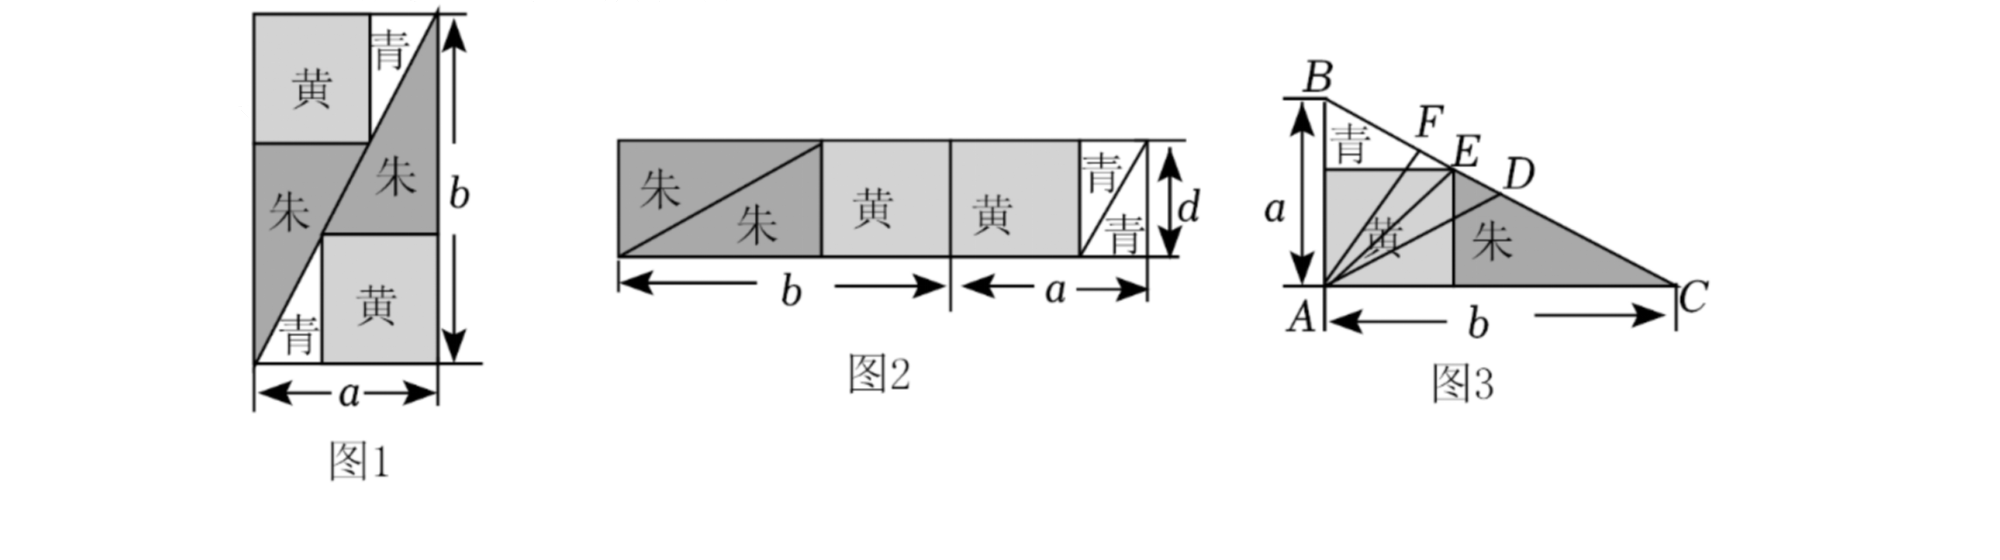
\includegraphics[width=0.86\textwidth]{figures/gao107_q11.png}
\end{center}

①由图 1 和图 2 面积相等得 $d=\dfrac{2ab}{a+b}$　　②由 $AE\geqslant AF$ 可得 $\sqrt{\dfrac{a^2+b^2}2}\geqslant\dfrac{a+b}2$

③由 $AD\geqslant AE$ 可得 $\sqrt{\dfrac{a^2+b^2}2}\geqslant\dfrac{2}{\dfrac1a+\dfrac1b}$　④由 $AD\geqslant AF$ 可得 $a^2+b^2\geqslant2ab$

\ifanswer
\solbegin
\step{对于①，由图 1 和图 2 面积相等得 $ab=(a+b)\times d$，所以 $d=\dfrac{ab}{a+b}$，故①错,}
\step{对于②，因为 $AF\perp BC$，所以 $\dfrac12ab=\dfrac12\sqrt{a^2+b^2}\times AF$,}
\step{所以 $AF=\dfrac{ab}{\sqrt{a^2+b^2}}$，$AE=\sqrt2d=\dfrac{\sqrt2ab}{a+b}$,}
\step{因为 $AE\geqslant AF$，所以 $\dfrac{\sqrt2ab}{a+b}\geqslant\dfrac{ab}{\sqrt{a^2+b^2}}$，整理得 $\sqrt{\dfrac{a^2+b^2}2}\geqslant\dfrac{a+b}2$，故②对,}
\step{对于③，因为 $D$ 是斜边 $BC$ 的中点，所以 $AD=\sqrt{\dfrac{a^2+b^2}2}$,}
\step{因为 $AD\geqslant AE$，所以 $\sqrt{\dfrac{a^2+b^2}2}\geqslant\dfrac{\sqrt2ab}{a+b}$，整理得 $\sqrt{\dfrac{a^2+b^2}2}\geqslant\dfrac{2}{\dfrac1a+\dfrac1b}$，故③对,}
\step{对于④，因为 $AD\geqslant AF$，所以 $\sqrt{\dfrac{a^2+b^2}2}\geqslant\dfrac{ab}{\sqrt{a^2+b^2}}$，整理得 $a^2+b^2\geqslant2ab$,}
\step{故④对,}
\step{故正确的是②③④.}
\solend
\fi

\item 设 $a,b,c,d\in\R$ 且$\lvert a-b\rvert\leqslant2$,$\lvert c-d\rvert\leqslant2$,$\lvert a\rvert\leqslant3$,$\lvert c\rvert\leqslant3$，则 $\lvert ad-bc\rvert$ 的最大值为\blankline[4.4em].% 原卷四处条件间均排半角逗号，照录

\ifanswer
\solbegin
\step{令 $a-b=e$,$c-d=f$，则 $\lvert e\rvert\leqslant2$,$\lvert f\rvert\leqslant2$,$\lvert a\rvert\leqslant3$,$\lvert c\rvert\leqslant3$}
\step{则 $\lvert ad-bc\rvert=\lvert a(c-f)-(a-e)c\rvert=\lvert ce-af\rvert\leqslant\lvert c\rvert\,\lvert e\rvert+\lvert a\rvert\,\lvert f\rvert\leqslant12$,}
\step{则 $\lvert ad-bc\rvert$ 的最大值为 12.}
\solend
\fi

\end{enumerate}

\bigsec{二、选择题}

\begin{enumerate}
\setcounter{enumi}{12}

\item 下列说法正确的是\mbox{（\quad）}

\keepwithprev
A. 若 $a>b>0$，则 $ac^2>bc^2$\qquad\qquad B. 若 $a<b<0$，则 $a^2>ab>b^2$

C. 若 $a>b$，则 $a^2>b^2$\qquad\qquad\qquad D. 若 $a<b$，则 $\dfrac1a>\dfrac1b$

\ifanswer
\solbegin
\step{$A$. 当 $a>b>0$ 时，取 $c=0$，则 $ac^2>bc^2$ 不成立，故 $A$ 错误；}
\step{$B$. 当 $a<b<0$ 时，由不等式的基本性质得 $a^2>ab>b^2>0$，故 $B$ 正确；}
\step{$C$. 当 $a>b$ 时，取 $a=0$，$b=-1$，则 $a^2>b^2$ 不成立，故 $C$ 错误；}
\step{$D$. 当 $a<b$ 时，取 $a=0$，$b=1$，则 $\dfrac1a>\dfrac1b$ 不成立，故 $D$ 错误.}
\step{故选 $B$.}
\solend
\fi

\item 小玲在学习《论语·子路》读到“其身正，不令而行；其身不正，虽令不从”，这句话的
数学含义可以理解为：“身正”是“令行”的\mbox{（\quad）}

\keepwithprev
A. 充分非必要条件\qquad\qquad B. 必要不充分条件

C. 充要条件\qquad\qquad\qquad D. 既非充分又非必要条件

\ifanswer
\solbegin
\step{其身正，不令而行，即身正$\Rightarrow$令行，所以“身正”是“令行”的充分条件；}
\step{又其身不正，虽令不从，即令行$\Rightarrow$身正，所以“身正”是“令行”的必要条件；}
\step{综上，“身正”是“令行”的充要条件. 故选 $C$.}
\solend
\fi

\item 某地对农户抽样调查，结果如下：电冰箱拥有率为 $45\%$，电视机拥有率为 $55\%$，洗衣
机拥有率为 $65\%$，拥有上述三种电器的任意两种的占 $35\%$，三种电器齐全的为 $25\%$，那
么一种电器也没有的农户所占比例是\mbox{（\quad）}

\keepwithprev
A. $12\%$\qquad B. $15\%$\qquad C. $18\%$\qquad D. $20\%$

\ifanswer
\solbegin
\step{设只有电冰箱和电视机的农户有 $a$ 家，只有电冰箱和洗衣机的农户有 $b$ 家,}
\step{只有洗衣机和电视机的农户有 $c$ 家,}
\step{只有电视机、电冰箱、洗衣机的分别有 $d$、$e$、$f$ 家,}
\step{没有任何电器的农户有 $x$ 家,}

\begin{center}
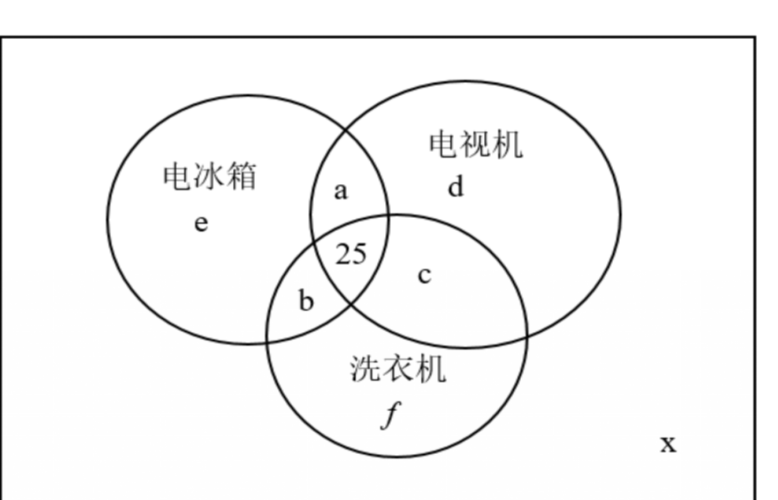
\includegraphics[width=0.42\textwidth]{figures/gao107_q15.png}
\end{center}

\step{所以 $25+a+b+e=45$①，$25+a+c+d=55$②,}
\step{$25+b+c+f=65$③,}
\step{把上面三个式子相加得 $2(a+b+c)+d+e+f=90$④,}
\step{对于拥有上述三种电器的任意两种的占 $35\%$，得 $a+b+c=35$⑤,}
\step{把⑤代入④可得到 $d+e+f=20$⑥,}
\step{因为农户共有 100 家，所以 $25+a+b+c+d+e+f+x=100$,}
\step{把⑤和⑥代入上式得 $x=20$，即一种电器也没有的农户所占比例为 $20\%$.}
\step{故选 $D$.}
\solend
\fi

\item 设 $d>0$，已知 $A,B$ 是两个数集. 若对任意 $x\in A$，都存在 $y\in B$，使得 $\lvert x-y\rvert<d$，则
称 $A$ 是 $B$ 的一个“$d-$邻集”. 现有下列两个命题：① $M=\{a+b\sqrt2\mid a,b\in\Z\}$ 是 $\Q$ 的一个
$\dfrac1{2025}$
一邻集；②若 $A$ 是 $B$ 的一个 $d-$邻集，则 $B$ 也是 $A$ 的一个 $d-$邻集；则\mbox{（\quad）}% 原卷把 d−邻集 的连字符断行后排成“一邻集”，照录

\keepwithprev
A. ①真②假\qquad B. ①假②真\qquad C. ①真②真\qquad D. ①假②假

\ifanswer
\solbegin
\step{对于①，任取 $M$ 中的元素 $x_0=a_0+b_0\sqrt2$,}
\step{则存在 $y_0\in\Q\cap\left(a_0+b_0\sqrt2-\dfrac1{2025},a_0+b_0\sqrt2+\dfrac1{2025}\right)$ 满足题意，故①正确；}
\step{对于②，取 $A=[-1,1]$,$B=[-2,2]$, $A$ 是 $B$ 的 $\dfrac12-$邻集，但反之不成立,}
\step{故②错误；}
\step{故选 $A$.}
\solend
\fi

\end{enumerate}

\bigsec{三、解答题}

\begin{enumerate}
\setcounter{enumi}{16}

\item 设 $a\in\R$，完成下列问题：

（1）求不等式 $3(a+1)x-3>2ax-3a$ 的解集 $M$；

（2）设集合 $A=\{x\mid x^2-ax+a^2-19=0\}$，$B=\{x\mid x^2-5x+6=0\}$，
$C=\{x\mid x^2+2x-8=0\}$. 若 $A\cap B\supset\varnothing$，$A\cap C=\varnothing$，求 $a$ 的值.

\ifanswer
\solbegin
\step{（1）不等式 $3(a+1)x-3>2ax-3a$ 可化为 $(a+3)x>3-3a$,}
\step{当 $a+3>0$，即 $a>-3$ 时，解得 $x>\dfrac{3-3a}{a+3}$,}
\step{当 $a+3=0$，即 $a=-3$ 时，不等式化为 $0\cdot x>12$，无解,}
\step{当 $a+3<0$，即 $a<-3$ 时，解得 $x<\dfrac{3-3a}{a+3}$,}
\step{综上所述，当 $a>-3$ 时，$M=\left(\dfrac{3-3a}{a+3},+\infty\right)$；}
\step{当 $a=-3$ 时，$M=\varnothing$；}
\step{当 $a<-3$ 时，$M=\left(-\infty,\dfrac{3-3a}{a+3}\right)$；}
\step{（2）$B=\{x\mid x^2-5x+6=0\}=\{2,3\}$，$C=\{x\mid x^2+2x-8=0\}=\{2,-4\}$,}
\step{因为 $A\cap B\supset\varnothing$，所以 $A\cap B\neq\varnothing$，又因为 $A\cap C=\varnothing$,}
\step{所以 $3\in A$，$2\notin A$，$-4\notin A$,}
\step{把 $x=3$ 代入方程 $x^2-ax+a^2-19=0$ 得 $9-3a+a^2-19=0$,}
\step{解得 $a=-2$ 或 $a=5$,}
\step{当 $a=-2$ 时，集合 $A=\{x\mid x^2+2x-15=0\}=\{3,-5\}$，符合题意,}
\step{当 $a=5$ 时，集合 $A=\{x\mid x^2-5x+6=0\}=\{3,2\}$，不符合题意，舍去,}
\step{综上所述，$a$ 的值为 $-2$.}
\solend
\fi

\item 完成下列问题：

（1）设 $x$、$y\in\R$，且 $x+y>5$，用反证法证明：$x>3$ 或 $y>2$；

（2）设 $x>0$，$a=x+1$，$b=\sqrt{x^2+7x+1}$，求 $\dfrac ba$ 的最大值.

\ifanswer
\solbegin
\step{（1）假设 $x\leqslant3$ 且 $y\leqslant2$，则 $x+y\leqslant3+2=5$，这与已知 $x+y>5$ 矛盾,}
\step{故 $x>3$ 或 $y>2$；}
\step{（2）$x>0$，$a=x+1$，$b=\sqrt{x^2+7x+1}$,}
\step{则 $\dfrac ba=\dfrac{\sqrt{x^2+7x+1}}{x+1}=\sqrt{\dfrac{x^2+7x+1}{x^2+2x+1}}=\sqrt{\dfrac{x^2+2x+1+5x}{x^2+2x+1}}$}
\step{$=\sqrt{1+\dfrac{5x}{x^2+2x+1}}=\sqrt{1+\dfrac{5}{x+\dfrac1x+2}}\leqslant\sqrt{1+\dfrac{5}{2\sqrt{x\cdot\dfrac1x}+2}}=\dfrac32$,}
\step{当且仅当 $x=\dfrac1x$，即 $x=1$ 时取等号，故 $\dfrac ba$ 的最大值为 $\dfrac32$.}
\solend
\fi

\item 已知函数 $f(x)=\lvert2x-a\rvert+a$.

（1）当 $a=2$ 时，求不等式 $f(x)\leqslant6+\lvert x+2\rvert$ 的解集；

（2）设 $g(x)=\lvert2x-1\rvert$，若不等式 $f(x)+g(x)\geqslant3$ 对一切 $x\in\R$ 恒成立，求实数 $a$ 的取值
范围.

\ifanswer
\solbegin
\ansspace*
\step{（1）$a=2$ 时，$f(x)=\lvert2x-2\rvert+2$,}
\step{则 $f(x)\leqslant6+\lvert x+2\rvert\Leftrightarrow\lvert2x-2\rvert+2\leqslant6+\lvert x+2\rvert$，即 $\lvert2x-2\rvert-\lvert x+2\rvert\leqslant4$,}
\step{当 $x<-2$ 时，$2-2x+x+2\leqslant4$，解得 $x\geqslant0$，与 $x<-2$ 取交集得 $\varnothing$,}
\step{当 $-2\leqslant x\leqslant1$ 时，$2-2x-x-2\leqslant4$，解得 $x\geqslant-\dfrac43$,}
\step{与 $-2\leqslant x\leqslant1$ 取交集得 $-\dfrac43\leqslant x\leqslant1$,}
\step{当 $x>1$ 时，$2x-2-x-2\leqslant4$，解得 $x\leqslant8$，与 $x>1$ 取交集得 $1<x\leqslant8$,}
\step{综上，不等式 $f(x)\leqslant6+\lvert x+2\rvert$ 的解集为 $\left\{x\,\middle|\,-\dfrac43\leqslant x\leqslant8\right\}$；}
\step{（2）$f(x)+g(x)\geqslant3$，即 $\lvert2x-a\rvert+a+\lvert2x-1\rvert\geqslant3$,}
\step{故 $\lvert2x-a\rvert+\lvert2x-1\rvert\geqslant3-a$,}
\step{当 $a\geqslant3$ 时，不等式显然成立,}
\step{当 $a<3$ 时,}
\step{由三角不等式得 $\lvert2x-a\rvert+\lvert2x-1\rvert\geqslant\lvert2x-a-(2x-1)\rvert=\lvert1-a\rvert$,}
\step{当且仅当 $(2x-a)(2x-1)\leqslant0$ 时取等号，因此 $\lvert1-a\rvert\geqslant3-a$,}
\step{平方得 $(1-a)^2\geqslant(3-a)^2$，解得 $a\geqslant2$，故 $2\leqslant a<3$.}
\step{综上，实数 $a$ 的取值范围是 $a\geqslant2$.}
\solend
\fi

\item 对于集合 $A,B$，定义集合 $A-B=\{x\mid x\in A$ 且 $x\notin B\}$.

（1）若 $A=\{1,2,3,4\}$,$B=\{3,4,5\}$，求集合 $A-B$ 和 $B-A$；

（2）给定集合 $A,B$，求所有满足方程组
\[
\begin{cases}
X\cap(A\cup B)=X\\
A\cap(B\cup X)=A\\
B\cap(A\cup X)=B\\
X\cap(A\cap B)=\varnothing
\end{cases}
\]
的集合 $X$（用 $A,B$ 表示）；

（3）用 $\lvert M\rvert$ 表示集合 $M$ 中的元素个数. 给定正整数 $n$，集合 $S=\{1,2,\cdots,n\}$. 对于实数
集的非空有限子集 $A,B$，定义集合 $C=\{x\mid x=a+b,a\in A,b\in B\}$. 求证：

$\lvert A-S\rvert+\lvert B-S\rvert+\lvert S-C\rvert\geqslant1$.

\ifanswer
\solbegin
\step{（1）由 $A=\{1,2,3,4\}$,$B=\{3,4,5\}$，则 $A-B=\{1,2\}$,$B-A=\{5\}$；}
\step{（2）由
$\begin{cases}
X\cap(A\cup B)=X\\
X\cap(A\cap B)=\varnothing
\end{cases}$，
得 $X\subseteq A-B$ 或 $X\subseteq B-A$,}
\step{再结合
$\begin{cases}
A\cap(B\cup X)=A\\
B\cap(A\cup X)=B
\end{cases}$，
得 $X=(A-B)\cup(B-A)$,}
\step{所以 $X=(A-B)\cup(B-A)$；}
\step{（3）$\lvert X\rvert$ 表示集合 $X$ 中的元素个数，则 $\lvert X\rvert\geqslant0$,}
\step{若 $A\cup B$ 中至少含有一个不在 $S$ 中的元素，则 $\lvert A-S\rvert+\lvert B-S\rvert\geqslant1$,}
\step{即 $\lvert A-S\rvert+\lvert B-S\rvert+\lvert S-C\rvert\geqslant1$.}
\step{若 $A\subseteq S$，且 $B\subseteq S$，则 $\lvert A-S\rvert=\lvert B-S\rvert=0$.}
\step{此时 $A$ 中最小的元素 $a\geqslant1$,$B$ 中最小的元素 $b\geqslant1$.}
\step{所以 $C$ 中最小的元素 $a+b\geqslant2$，则 $1\notin C$,}
\step{因为 $S=\{1,2,\cdots,n\}$，所以 $\lvert S-C\rvert\geqslant1$，即 $\lvert A-S\rvert+\lvert B-S\rvert+\lvert S-C\rvert\geqslant1$.}
\step{综上所述，$\lvert A-S\rvert+\lvert B-S\rvert+\lvert S-C\rvert\geqslant1$.}
\solend
\fi

\end{enumerate}

\end{document}
"
% 紧凑版：xelatex "\def\iscompact{1}% 高一107_曹杨二中_10月月考.tex
%   —— 高一上数学“2026-2027 年曹杨二中高一上 10 月月考”（试卷版/答案版）
% 试卷版：xelatex 高一107_曹杨二中_10月月考.tex
% 答案版：xelatex "\def\isanswer{1}\input{高一107_曹杨二中_10月月考.tex}"
% 紧凑版：xelatex "\def\iscompact{1}\input{高一107_曹杨二中_10月月考.tex}"
%
% 原始材料：微信公众号“魔都数学加油站”文章，作者破晓，2026-11-03 17:19 发布；
% 连载“27学年高一107”，原文标题“27学年高一107——2026-2027年上海市曹杨二中高一上10月月考”；
% 原文链接：https://mp.weixin.qq.com/s/IF4uB7aDNv-snYwbGMoDiQ。
% 正文为 10 张 PNG 页（第 1、2、4、6—9 页 4762×6735，第 3、5、10 页 2560×3620），题目下印有【解析】，为讲评版。
% 题目、解析均据原图转录；卷面水印及公众号页脚未录入。
% 第 11 题题干的三幅“出入相补”图（图 1—图 3）与第 15 题解析的三圆文氏图裁自原图、
% 去粉色水印转灰度（gao107_q11.png、gao107_q15.png），第 11 题图属题干（三版都出）、
% 第 15 题图属解析（仅答案版显示）。
%
% 卷首标题：原卷印作“2026-2027 年曹杨二中高一上 10 月月考”（公众号标题中的“上海市”
% 卷面标题行没有，本稿照卷面），年份区间按全稿惯例排 en dash；原卷未印副标题，本稿按题目内容
% 标为“集合与常用逻辑用语、不等式”。
%
% 与原卷的排版差异：
%   ① 原文从第 3 题起，填空题编号为 3—12、选择题为 13—16、解答题为 17—20，本稿保留原题号；
%   ② 原卷每题下直接印【解析】，本稿按全稿惯例将解析置于答案版；第 4 题只印【答案】另提 \ans{}；
%   ③ 原卷未印副标题，本稿按“知识模块”口径补出；
%   ④ 原卷填空横线按全稿惯例排为 \blankline[4.4em]；解答题按惯例加 \ansspace；选择题括号排
%      \mbox{（\quad）}、选项段前按惯例加 \keepwithprev；
%   ⑤ 原卷数集字母粗体与斜体混用（第 3 题 $\mathbf{R}$、第 4 题斜体 $R$、第 16 题粗体
%      $\mathbf{Z}$、$\mathbf{Q}$ 等），按全稿惯例统一改 \R、\Z、\Q。
%
% 原卷存疑：第 10 题解析“由 $\Delta=16m^2-8(2m^2+3m-2)\geqslant0$ 得 $m\leqslant\dfrac23$”
% 行末原卷无句读，照录。第 16 题解析②“取 $A=[-1,1]$，$B=[-2,2]$，$A$ 是 $B$ 的
% $\dfrac12$-邻集，但反之不成立”，据以判①真②假，照录。
%
% 行数核对：逐题数 \step/\stepm 条数，合计 112 条（Q3：5；Q4：0；Q5：2；Q6：2；Q7：2；
% Q8：4；Q9：8；Q10：4；Q11：9；Q12：3；Q13：5；Q14：3；Q15：12；Q16：5；Q17：15；
% Q18：6；Q19：15；Q20：12），与原卷印刷行逐题相等。第 4 题只印【答案】，提 \ans{}，
% 不计入 \step 账。
%
\documentclass[a4paper,11pt]{article}
\usepackage{common}

\begin{document}

\examtitlest[3]{2026--2027 年曹杨二中高一上 10 月月考}{集合与常用逻辑用语、不等式}

\bigsec{一、填空题}

\begin{enumerate}
\setcounter{enumi}{2}

\item 设 $a\in\R$，若 $3\in\{\sqrt3,a^2,a\}$，则 $a=$\blankline[4.4em].

\ifanswer
\solbegin
\step{因为 $3\in\{\sqrt3,a^2,a\}$，所以 $a^2=3$，解得 $a=\sqrt3$ 或 $a=-\sqrt3$,}
\step{当 $a=\sqrt3$ 时，集合为 $\{\sqrt3,3,\sqrt3\}$，不满足集合元素的互异性，舍去；}
\step{当 $a=-\sqrt3$ 时，集合为 $\{\sqrt3,3,-\sqrt3\}$，符合要求；}
\step{若 $a=3$，此时集合为 $\{\sqrt3,9,3\}$，符合要求；}
\step{综上，$a$ 为 $-\sqrt3$ 或 $3$.}
\solend
\fi

\item 设 $a\in\R$，已知集合 $A=\{x\mid x\leqslant a\}$，$B=\{x\mid x>2\}$. 若 $A\cup B=\R$，则 $a$ 的取值范围是\blankline[4.4em].

\ifanswer
\ans{$a\geqslant2$}
\fi

\item 设 $x>0$，$y>0$ 且 $x+3y=1$，则 $xy$ 的最大值为\blankline[4.4em].

\ifanswer
\solbegin
\step{由于 $x>0$，$y>0$ 且 $x+3y=1$，则 $1=x+3y\geqslant2\sqrt{3xy}$，得 $xy\leqslant\dfrac1{12}$,}
\step{当且仅当 $x=3y=\dfrac12$ 时取等号，则 $xy$ 的最大值为 $\dfrac1{12}$.}
\solend
\fi

\item 设 $a\in\R$，若集合$\left\{x\,\middle|\,\dfrac{ax}{x-1}=x\right\}$有且仅有两个子集，则 $a=$\blankline[4.4em].

\ifanswer
\solbegin
\step{由 $\dfrac{ax}{x-1}=x$ 得 $ax=x(x-1)$，即 $x(x-a-1)=0$,}
\step{所以此方程有两个相等的（不等于 1）的实数根或有一根为 1，所以 $a=-1$ 或 $0$.}
\solend
\fi

\item 已知全集 $U=\{x\mid x^2-8x-20<0\}$，集合 $A=\{x\mid 1-x^2>0$ 且 $x<0\}$，则 $\overline A=$\blankline[4.4em].

\ifanswer
\solbegin
\step{$U=\{x\mid-2<x<10\}$，$A=\{x\mid-1<x<0\}$,}
\step{所以 $\overline A=\{x\mid-2<x\leqslant-1$ 或 $0\leqslant x<10\}$.}
\solend
\fi

\item 设 $a,b\in\R$，若不等式 $-x^2-ax+b\geqslant0$ 的解集为 $[-2,3]$，则不等式 $\lvert ax+b\rvert<5$ 的解集为\blankline[4.4em].

\ifanswer
\solbegin
\step{由不等式 $-x^2-ax+b\geqslant0$ 的解集为 $[-2,3]$,}
\step{得 $-2$、$3$ 是方程 $-x^2-ax+b=0$ 的两个根，所以 $a=-1$，$b=6$.}
\step{解不等式 $\lvert-x+6\rvert<5$，得 $-5<x-6<5$，解得 $1<x<11$,}
\step{即所求不等式的解集为 $(1,11)$.}
\solend
\fi

\item 某货运卡车以 $x$ 千米／时的速度匀速行驶 300 千米，按交通法规限制 $50\leqslant x\leqslant100$，假设
柴油的价格为每升 6 元，汽车每小时耗油 $\left(4+\dfrac{x^2}{420}\right)$ 升，司机工资为每小时 46 元. 则当
$x=$\blankline[4.4em]（千米／时），这次行车的总费用（油费与司机工资的总和）最低.

\ifanswer
\solbegin
\step{因为卡车行驶 300 千米，速度为 $x$ 千米／时,}
\step{因此总用时为 $t=\dfrac{300}{x}$ 小时，其中 $50\leqslant x\leqslant100$,}
\step{每小时油费为 $6\cdot\left(4+\dfrac{x^2}{420}\right)$ 元，每小时司机工资为 46 元，因}
\step{此每小时总支出为 $6\cdot\left(4+\dfrac{x^2}{420}\right)+46=70+\dfrac{x^2}{70}$ 元.}
\step{设全程总费用为 $y$，则 $y=\dfrac{300}{x}\cdot\left(70+\dfrac{x^2}{70}\right)=\dfrac{21000}{x}+\dfrac{30x}{7}$,}
\step{因为 $50\leqslant x\leqslant100$，$\dfrac{21000}{x}+\dfrac{30x}{7}\geqslant2\sqrt{\dfrac{21000}{x}\cdot\dfrac{30x}{7}}=600$,}
\step{当且仅当 $\dfrac{21000}{x}=\dfrac{30x}{7}$，即 $x=70$ 时取等号，且 $70\in[50,100]$,}
\step{因此当 $x=70$ 千米／时，行车的总费用（油费与司机工资的总和）最低.}
\solend
\fi

\item 设 $x_1$、$x_2$ 是关于 $x$ 的方程 $2x^2-4mx+2m^2+3m-2=0$ 的两个实数根，则 $x_1^2+x_2^2$ 的最小值为\blankline[4.4em].

\ifanswer
\solbegin
\step{由题意得 $x_1+x_2=2m$，$x_1x_2=m^2+\dfrac{3m}{2}-1$,}
\step{由 $\Delta=16m^2-8(2m^2+3m-2)\geqslant0$ 得 $m\leqslant\dfrac23$}
\step{所以 $x_1^2+x_1^2=(x_1+x_2)^2-2x_1x_2=4m^2-2m^2+3m+2=2m^2-3m+2$,% 原卷左端作 x_1²+x_1²，照录
}
\step{结合二次函数的性质得，当 $m=\dfrac23$ 时取得最小值 $\dfrac89$.}
\solend
\fi

\item 小玲在钻研《九章算术》中“勾股容方”问题“今有勾五步，股十二步，问勾中容方几
何？”时，发现魏晋时期数学家刘徽在其《九章算术注》中利用出入相补原理给出了这个
问题的一般解法：如图 1，用对角线将长和宽分别为 $b$ 和 $a$ 的矩形分成两个直角三角形，
每个直角三角形再分成一个内接正方形（黄）和两个小直角三角形（朱、青）. 将三种颜色
的图形进行重组，得到如图 2 所示的矩形，该矩形长为 $a+b$，宽为内接正方形的边长
$d$. 由刘徽构造的图形可以得到许多重要的结论，如图 3，设 $D$ 为斜边 $BC$ 的中点，作直
角三角形 $ABC$ 的内接正方形对角线 $AE$，过点 $A$ 作 $AF\perp BC$ 于点 $F$，则下列四个推理中
正确的序号是\blankline[4.4em].

\begin{center}
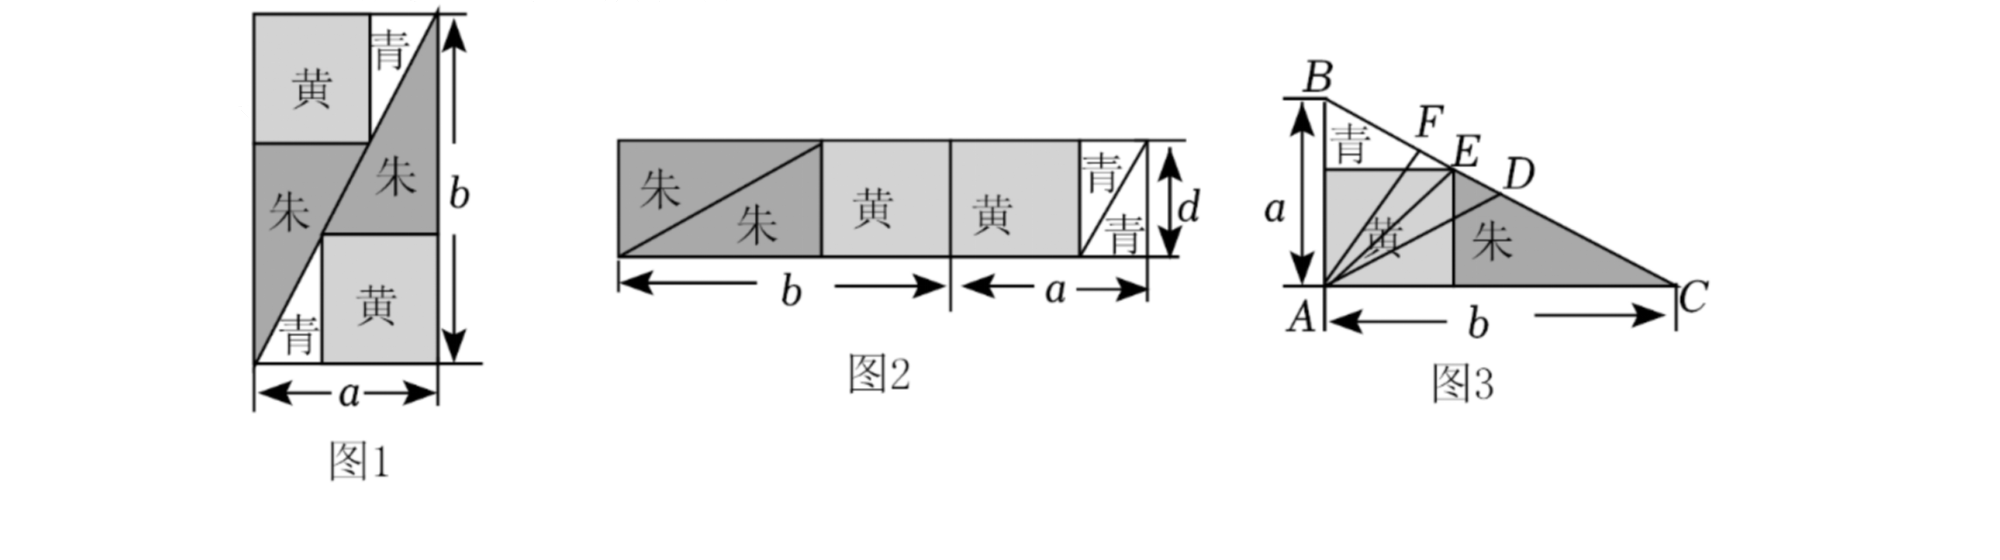
\includegraphics[width=0.86\textwidth]{figures/gao107_q11.png}
\end{center}

①由图 1 和图 2 面积相等得 $d=\dfrac{2ab}{a+b}$　　②由 $AE\geqslant AF$ 可得 $\sqrt{\dfrac{a^2+b^2}2}\geqslant\dfrac{a+b}2$

③由 $AD\geqslant AE$ 可得 $\sqrt{\dfrac{a^2+b^2}2}\geqslant\dfrac{2}{\dfrac1a+\dfrac1b}$　④由 $AD\geqslant AF$ 可得 $a^2+b^2\geqslant2ab$

\ifanswer
\solbegin
\step{对于①，由图 1 和图 2 面积相等得 $ab=(a+b)\times d$，所以 $d=\dfrac{ab}{a+b}$，故①错,}
\step{对于②，因为 $AF\perp BC$，所以 $\dfrac12ab=\dfrac12\sqrt{a^2+b^2}\times AF$,}
\step{所以 $AF=\dfrac{ab}{\sqrt{a^2+b^2}}$，$AE=\sqrt2d=\dfrac{\sqrt2ab}{a+b}$,}
\step{因为 $AE\geqslant AF$，所以 $\dfrac{\sqrt2ab}{a+b}\geqslant\dfrac{ab}{\sqrt{a^2+b^2}}$，整理得 $\sqrt{\dfrac{a^2+b^2}2}\geqslant\dfrac{a+b}2$，故②对,}
\step{对于③，因为 $D$ 是斜边 $BC$ 的中点，所以 $AD=\sqrt{\dfrac{a^2+b^2}2}$,}
\step{因为 $AD\geqslant AE$，所以 $\sqrt{\dfrac{a^2+b^2}2}\geqslant\dfrac{\sqrt2ab}{a+b}$，整理得 $\sqrt{\dfrac{a^2+b^2}2}\geqslant\dfrac{2}{\dfrac1a+\dfrac1b}$，故③对,}
\step{对于④，因为 $AD\geqslant AF$，所以 $\sqrt{\dfrac{a^2+b^2}2}\geqslant\dfrac{ab}{\sqrt{a^2+b^2}}$，整理得 $a^2+b^2\geqslant2ab$,}
\step{故④对,}
\step{故正确的是②③④.}
\solend
\fi

\item 设 $a,b,c,d\in\R$ 且$\lvert a-b\rvert\leqslant2$,$\lvert c-d\rvert\leqslant2$,$\lvert a\rvert\leqslant3$,$\lvert c\rvert\leqslant3$，则 $\lvert ad-bc\rvert$ 的最大值为\blankline[4.4em].% 原卷四处条件间均排半角逗号，照录

\ifanswer
\solbegin
\step{令 $a-b=e$,$c-d=f$，则 $\lvert e\rvert\leqslant2$,$\lvert f\rvert\leqslant2$,$\lvert a\rvert\leqslant3$,$\lvert c\rvert\leqslant3$}
\step{则 $\lvert ad-bc\rvert=\lvert a(c-f)-(a-e)c\rvert=\lvert ce-af\rvert\leqslant\lvert c\rvert\,\lvert e\rvert+\lvert a\rvert\,\lvert f\rvert\leqslant12$,}
\step{则 $\lvert ad-bc\rvert$ 的最大值为 12.}
\solend
\fi

\end{enumerate}

\bigsec{二、选择题}

\begin{enumerate}
\setcounter{enumi}{12}

\item 下列说法正确的是\mbox{（\quad）}

\keepwithprev
A. 若 $a>b>0$，则 $ac^2>bc^2$\qquad\qquad B. 若 $a<b<0$，则 $a^2>ab>b^2$

C. 若 $a>b$，则 $a^2>b^2$\qquad\qquad\qquad D. 若 $a<b$，则 $\dfrac1a>\dfrac1b$

\ifanswer
\solbegin
\step{$A$. 当 $a>b>0$ 时，取 $c=0$，则 $ac^2>bc^2$ 不成立，故 $A$ 错误；}
\step{$B$. 当 $a<b<0$ 时，由不等式的基本性质得 $a^2>ab>b^2>0$，故 $B$ 正确；}
\step{$C$. 当 $a>b$ 时，取 $a=0$，$b=-1$，则 $a^2>b^2$ 不成立，故 $C$ 错误；}
\step{$D$. 当 $a<b$ 时，取 $a=0$，$b=1$，则 $\dfrac1a>\dfrac1b$ 不成立，故 $D$ 错误.}
\step{故选 $B$.}
\solend
\fi

\item 小玲在学习《论语·子路》读到“其身正，不令而行；其身不正，虽令不从”，这句话的
数学含义可以理解为：“身正”是“令行”的\mbox{（\quad）}

\keepwithprev
A. 充分非必要条件\qquad\qquad B. 必要不充分条件

C. 充要条件\qquad\qquad\qquad D. 既非充分又非必要条件

\ifanswer
\solbegin
\step{其身正，不令而行，即身正$\Rightarrow$令行，所以“身正”是“令行”的充分条件；}
\step{又其身不正，虽令不从，即令行$\Rightarrow$身正，所以“身正”是“令行”的必要条件；}
\step{综上，“身正”是“令行”的充要条件. 故选 $C$.}
\solend
\fi

\item 某地对农户抽样调查，结果如下：电冰箱拥有率为 $45\%$，电视机拥有率为 $55\%$，洗衣
机拥有率为 $65\%$，拥有上述三种电器的任意两种的占 $35\%$，三种电器齐全的为 $25\%$，那
么一种电器也没有的农户所占比例是\mbox{（\quad）}

\keepwithprev
A. $12\%$\qquad B. $15\%$\qquad C. $18\%$\qquad D. $20\%$

\ifanswer
\solbegin
\step{设只有电冰箱和电视机的农户有 $a$ 家，只有电冰箱和洗衣机的农户有 $b$ 家,}
\step{只有洗衣机和电视机的农户有 $c$ 家,}
\step{只有电视机、电冰箱、洗衣机的分别有 $d$、$e$、$f$ 家,}
\step{没有任何电器的农户有 $x$ 家,}

\begin{center}
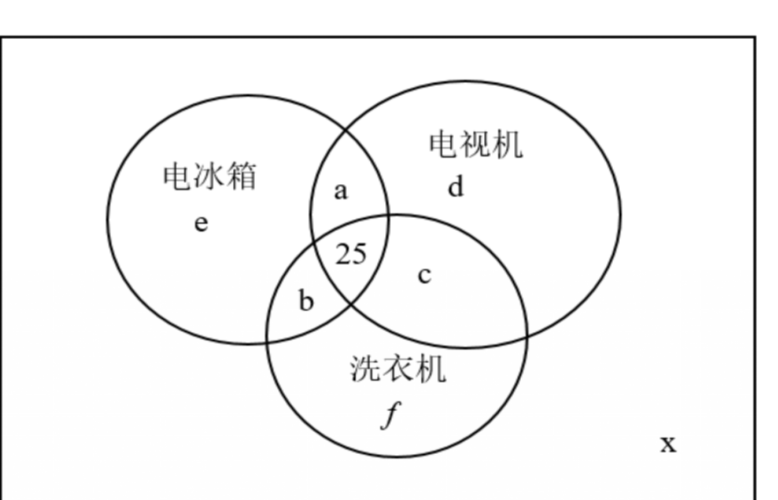
\includegraphics[width=0.42\textwidth]{figures/gao107_q15.png}
\end{center}

\step{所以 $25+a+b+e=45$①，$25+a+c+d=55$②,}
\step{$25+b+c+f=65$③,}
\step{把上面三个式子相加得 $2(a+b+c)+d+e+f=90$④,}
\step{对于拥有上述三种电器的任意两种的占 $35\%$，得 $a+b+c=35$⑤,}
\step{把⑤代入④可得到 $d+e+f=20$⑥,}
\step{因为农户共有 100 家，所以 $25+a+b+c+d+e+f+x=100$,}
\step{把⑤和⑥代入上式得 $x=20$，即一种电器也没有的农户所占比例为 $20\%$.}
\step{故选 $D$.}
\solend
\fi

\item 设 $d>0$，已知 $A,B$ 是两个数集. 若对任意 $x\in A$，都存在 $y\in B$，使得 $\lvert x-y\rvert<d$，则
称 $A$ 是 $B$ 的一个“$d-$邻集”. 现有下列两个命题：① $M=\{a+b\sqrt2\mid a,b\in\Z\}$ 是 $\Q$ 的一个
$\dfrac1{2025}$
一邻集；②若 $A$ 是 $B$ 的一个 $d-$邻集，则 $B$ 也是 $A$ 的一个 $d-$邻集；则\mbox{（\quad）}% 原卷把 d−邻集 的连字符断行后排成“一邻集”，照录

\keepwithprev
A. ①真②假\qquad B. ①假②真\qquad C. ①真②真\qquad D. ①假②假

\ifanswer
\solbegin
\step{对于①，任取 $M$ 中的元素 $x_0=a_0+b_0\sqrt2$,}
\step{则存在 $y_0\in\Q\cap\left(a_0+b_0\sqrt2-\dfrac1{2025},a_0+b_0\sqrt2+\dfrac1{2025}\right)$ 满足题意，故①正确；}
\step{对于②，取 $A=[-1,1]$,$B=[-2,2]$, $A$ 是 $B$ 的 $\dfrac12-$邻集，但反之不成立,}
\step{故②错误；}
\step{故选 $A$.}
\solend
\fi

\end{enumerate}

\bigsec{三、解答题}

\begin{enumerate}
\setcounter{enumi}{16}

\item 设 $a\in\R$，完成下列问题：

（1）求不等式 $3(a+1)x-3>2ax-3a$ 的解集 $M$；

（2）设集合 $A=\{x\mid x^2-ax+a^2-19=0\}$，$B=\{x\mid x^2-5x+6=0\}$，
$C=\{x\mid x^2+2x-8=0\}$. 若 $A\cap B\supset\varnothing$，$A\cap C=\varnothing$，求 $a$ 的值.

\ifanswer
\solbegin
\step{（1）不等式 $3(a+1)x-3>2ax-3a$ 可化为 $(a+3)x>3-3a$,}
\step{当 $a+3>0$，即 $a>-3$ 时，解得 $x>\dfrac{3-3a}{a+3}$,}
\step{当 $a+3=0$，即 $a=-3$ 时，不等式化为 $0\cdot x>12$，无解,}
\step{当 $a+3<0$，即 $a<-3$ 时，解得 $x<\dfrac{3-3a}{a+3}$,}
\step{综上所述，当 $a>-3$ 时，$M=\left(\dfrac{3-3a}{a+3},+\infty\right)$；}
\step{当 $a=-3$ 时，$M=\varnothing$；}
\step{当 $a<-3$ 时，$M=\left(-\infty,\dfrac{3-3a}{a+3}\right)$；}
\step{（2）$B=\{x\mid x^2-5x+6=0\}=\{2,3\}$，$C=\{x\mid x^2+2x-8=0\}=\{2,-4\}$,}
\step{因为 $A\cap B\supset\varnothing$，所以 $A\cap B\neq\varnothing$，又因为 $A\cap C=\varnothing$,}
\step{所以 $3\in A$，$2\notin A$，$-4\notin A$,}
\step{把 $x=3$ 代入方程 $x^2-ax+a^2-19=0$ 得 $9-3a+a^2-19=0$,}
\step{解得 $a=-2$ 或 $a=5$,}
\step{当 $a=-2$ 时，集合 $A=\{x\mid x^2+2x-15=0\}=\{3,-5\}$，符合题意,}
\step{当 $a=5$ 时，集合 $A=\{x\mid x^2-5x+6=0\}=\{3,2\}$，不符合题意，舍去,}
\step{综上所述，$a$ 的值为 $-2$.}
\solend
\fi

\item 完成下列问题：

（1）设 $x$、$y\in\R$，且 $x+y>5$，用反证法证明：$x>3$ 或 $y>2$；

（2）设 $x>0$，$a=x+1$，$b=\sqrt{x^2+7x+1}$，求 $\dfrac ba$ 的最大值.

\ifanswer
\solbegin
\step{（1）假设 $x\leqslant3$ 且 $y\leqslant2$，则 $x+y\leqslant3+2=5$，这与已知 $x+y>5$ 矛盾,}
\step{故 $x>3$ 或 $y>2$；}
\step{（2）$x>0$，$a=x+1$，$b=\sqrt{x^2+7x+1}$,}
\step{则 $\dfrac ba=\dfrac{\sqrt{x^2+7x+1}}{x+1}=\sqrt{\dfrac{x^2+7x+1}{x^2+2x+1}}=\sqrt{\dfrac{x^2+2x+1+5x}{x^2+2x+1}}$}
\step{$=\sqrt{1+\dfrac{5x}{x^2+2x+1}}=\sqrt{1+\dfrac{5}{x+\dfrac1x+2}}\leqslant\sqrt{1+\dfrac{5}{2\sqrt{x\cdot\dfrac1x}+2}}=\dfrac32$,}
\step{当且仅当 $x=\dfrac1x$，即 $x=1$ 时取等号，故 $\dfrac ba$ 的最大值为 $\dfrac32$.}
\solend
\fi

\item 已知函数 $f(x)=\lvert2x-a\rvert+a$.

（1）当 $a=2$ 时，求不等式 $f(x)\leqslant6+\lvert x+2\rvert$ 的解集；

（2）设 $g(x)=\lvert2x-1\rvert$，若不等式 $f(x)+g(x)\geqslant3$ 对一切 $x\in\R$ 恒成立，求实数 $a$ 的取值
范围.

\ifanswer
\solbegin
\ansspace*
\step{（1）$a=2$ 时，$f(x)=\lvert2x-2\rvert+2$,}
\step{则 $f(x)\leqslant6+\lvert x+2\rvert\Leftrightarrow\lvert2x-2\rvert+2\leqslant6+\lvert x+2\rvert$，即 $\lvert2x-2\rvert-\lvert x+2\rvert\leqslant4$,}
\step{当 $x<-2$ 时，$2-2x+x+2\leqslant4$，解得 $x\geqslant0$，与 $x<-2$ 取交集得 $\varnothing$,}
\step{当 $-2\leqslant x\leqslant1$ 时，$2-2x-x-2\leqslant4$，解得 $x\geqslant-\dfrac43$,}
\step{与 $-2\leqslant x\leqslant1$ 取交集得 $-\dfrac43\leqslant x\leqslant1$,}
\step{当 $x>1$ 时，$2x-2-x-2\leqslant4$，解得 $x\leqslant8$，与 $x>1$ 取交集得 $1<x\leqslant8$,}
\step{综上，不等式 $f(x)\leqslant6+\lvert x+2\rvert$ 的解集为 $\left\{x\,\middle|\,-\dfrac43\leqslant x\leqslant8\right\}$；}
\step{（2）$f(x)+g(x)\geqslant3$，即 $\lvert2x-a\rvert+a+\lvert2x-1\rvert\geqslant3$,}
\step{故 $\lvert2x-a\rvert+\lvert2x-1\rvert\geqslant3-a$,}
\step{当 $a\geqslant3$ 时，不等式显然成立,}
\step{当 $a<3$ 时,}
\step{由三角不等式得 $\lvert2x-a\rvert+\lvert2x-1\rvert\geqslant\lvert2x-a-(2x-1)\rvert=\lvert1-a\rvert$,}
\step{当且仅当 $(2x-a)(2x-1)\leqslant0$ 时取等号，因此 $\lvert1-a\rvert\geqslant3-a$,}
\step{平方得 $(1-a)^2\geqslant(3-a)^2$，解得 $a\geqslant2$，故 $2\leqslant a<3$.}
\step{综上，实数 $a$ 的取值范围是 $a\geqslant2$.}
\solend
\fi

\item 对于集合 $A,B$，定义集合 $A-B=\{x\mid x\in A$ 且 $x\notin B\}$.

（1）若 $A=\{1,2,3,4\}$,$B=\{3,4,5\}$，求集合 $A-B$ 和 $B-A$；

（2）给定集合 $A,B$，求所有满足方程组
\[
\begin{cases}
X\cap(A\cup B)=X\\
A\cap(B\cup X)=A\\
B\cap(A\cup X)=B\\
X\cap(A\cap B)=\varnothing
\end{cases}
\]
的集合 $X$（用 $A,B$ 表示）；

（3）用 $\lvert M\rvert$ 表示集合 $M$ 中的元素个数. 给定正整数 $n$，集合 $S=\{1,2,\cdots,n\}$. 对于实数
集的非空有限子集 $A,B$，定义集合 $C=\{x\mid x=a+b,a\in A,b\in B\}$. 求证：

$\lvert A-S\rvert+\lvert B-S\rvert+\lvert S-C\rvert\geqslant1$.

\ifanswer
\solbegin
\step{（1）由 $A=\{1,2,3,4\}$,$B=\{3,4,5\}$，则 $A-B=\{1,2\}$,$B-A=\{5\}$；}
\step{（2）由
$\begin{cases}
X\cap(A\cup B)=X\\
X\cap(A\cap B)=\varnothing
\end{cases}$，
得 $X\subseteq A-B$ 或 $X\subseteq B-A$,}
\step{再结合
$\begin{cases}
A\cap(B\cup X)=A\\
B\cap(A\cup X)=B
\end{cases}$，
得 $X=(A-B)\cup(B-A)$,}
\step{所以 $X=(A-B)\cup(B-A)$；}
\step{（3）$\lvert X\rvert$ 表示集合 $X$ 中的元素个数，则 $\lvert X\rvert\geqslant0$,}
\step{若 $A\cup B$ 中至少含有一个不在 $S$ 中的元素，则 $\lvert A-S\rvert+\lvert B-S\rvert\geqslant1$,}
\step{即 $\lvert A-S\rvert+\lvert B-S\rvert+\lvert S-C\rvert\geqslant1$.}
\step{若 $A\subseteq S$，且 $B\subseteq S$，则 $\lvert A-S\rvert=\lvert B-S\rvert=0$.}
\step{此时 $A$ 中最小的元素 $a\geqslant1$,$B$ 中最小的元素 $b\geqslant1$.}
\step{所以 $C$ 中最小的元素 $a+b\geqslant2$，则 $1\notin C$,}
\step{因为 $S=\{1,2,\cdots,n\}$，所以 $\lvert S-C\rvert\geqslant1$，即 $\lvert A-S\rvert+\lvert B-S\rvert+\lvert S-C\rvert\geqslant1$.}
\step{综上所述，$\lvert A-S\rvert+\lvert B-S\rvert+\lvert S-C\rvert\geqslant1$.}
\solend
\fi

\end{enumerate}

\end{document}
"
%
% 原始材料：微信公众号“魔都数学加油站”文章，作者破晓，2026-11-03 17:19 发布；
% 连载“27学年高一107”，原文标题“27学年高一107——2026-2027年上海市曹杨二中高一上10月月考”；
% 原文链接：https://mp.weixin.qq.com/s/IF4uB7aDNv-snYwbGMoDiQ。
% 正文为 10 张 PNG 页（第 1、2、4、6—9 页 4762×6735，第 3、5、10 页 2560×3620），题目下印有【解析】，为讲评版。
% 题目、解析均据原图转录；卷面水印及公众号页脚未录入。
% 第 11 题题干的三幅“出入相补”图（图 1—图 3）与第 15 题解析的三圆文氏图裁自原图、
% 去粉色水印转灰度（gao107_q11.png、gao107_q15.png），第 11 题图属题干（三版都出）、
% 第 15 题图属解析（仅答案版显示）。
%
% 卷首标题：原卷印作“2026-2027 年曹杨二中高一上 10 月月考”（公众号标题中的“上海市”
% 卷面标题行没有，本稿照卷面），年份区间按全稿惯例排 en dash；原卷未印副标题，本稿按题目内容
% 标为“集合与常用逻辑用语、不等式”。
%
% 与原卷的排版差异：
%   ① 原文从第 3 题起，填空题编号为 3—12、选择题为 13—16、解答题为 17—20，本稿保留原题号；
%   ② 原卷每题下直接印【解析】，本稿按全稿惯例将解析置于答案版；第 4 题只印【答案】另提 \ans{}；
%   ③ 原卷未印副标题，本稿按“知识模块”口径补出；
%   ④ 原卷填空横线按全稿惯例排为 \blankline[4.4em]；解答题按惯例加 \ansspace；选择题括号排
%      \mbox{（\quad）}、选项段前按惯例加 \keepwithprev；
%   ⑤ 原卷数集字母粗体与斜体混用（第 3 题 $\mathbf{R}$、第 4 题斜体 $R$、第 16 题粗体
%      $\mathbf{Z}$、$\mathbf{Q}$ 等），按全稿惯例统一改 \R、\Z、\Q。
%
% 原卷存疑：第 10 题解析“由 $\Delta=16m^2-8(2m^2+3m-2)\geqslant0$ 得 $m\leqslant\dfrac23$”
% 行末原卷无句读，照录。第 16 题解析②“取 $A=[-1,1]$，$B=[-2,2]$，$A$ 是 $B$ 的
% $\dfrac12$-邻集，但反之不成立”，据以判①真②假，照录。
%
% 行数核对：逐题数 \step/\stepm 条数，合计 112 条（Q3：5；Q4：0；Q5：2；Q6：2；Q7：2；
% Q8：4；Q9：8；Q10：4；Q11：9；Q12：3；Q13：5；Q14：3；Q15：12；Q16：5；Q17：15；
% Q18：6；Q19：15；Q20：12），与原卷印刷行逐题相等。第 4 题只印【答案】，提 \ans{}，
% 不计入 \step 账。
%
\documentclass[a4paper,11pt]{article}
\usepackage{common}

\begin{document}

\examtitlest[3]{2026--2027 年曹杨二中高一上 10 月月考}{集合与常用逻辑用语、不等式}

\bigsec{一、填空题}

\begin{enumerate}
\setcounter{enumi}{2}

\item 设 $a\in\R$，若 $3\in\{\sqrt3,a^2,a\}$，则 $a=$\blankline[4.4em].

\ifanswer
\solbegin
\step{因为 $3\in\{\sqrt3,a^2,a\}$，所以 $a^2=3$，解得 $a=\sqrt3$ 或 $a=-\sqrt3$,}
\step{当 $a=\sqrt3$ 时，集合为 $\{\sqrt3,3,\sqrt3\}$，不满足集合元素的互异性，舍去；}
\step{当 $a=-\sqrt3$ 时，集合为 $\{\sqrt3,3,-\sqrt3\}$，符合要求；}
\step{若 $a=3$，此时集合为 $\{\sqrt3,9,3\}$，符合要求；}
\step{综上，$a$ 为 $-\sqrt3$ 或 $3$.}
\solend
\fi

\item 设 $a\in\R$，已知集合 $A=\{x\mid x\leqslant a\}$，$B=\{x\mid x>2\}$. 若 $A\cup B=\R$，则 $a$ 的取值范围是\blankline[4.4em].

\ifanswer
\ans{$a\geqslant2$}
\fi

\item 设 $x>0$，$y>0$ 且 $x+3y=1$，则 $xy$ 的最大值为\blankline[4.4em].

\ifanswer
\solbegin
\step{由于 $x>0$，$y>0$ 且 $x+3y=1$，则 $1=x+3y\geqslant2\sqrt{3xy}$，得 $xy\leqslant\dfrac1{12}$,}
\step{当且仅当 $x=3y=\dfrac12$ 时取等号，则 $xy$ 的最大值为 $\dfrac1{12}$.}
\solend
\fi

\item 设 $a\in\R$，若集合$\left\{x\,\middle|\,\dfrac{ax}{x-1}=x\right\}$有且仅有两个子集，则 $a=$\blankline[4.4em].

\ifanswer
\solbegin
\step{由 $\dfrac{ax}{x-1}=x$ 得 $ax=x(x-1)$，即 $x(x-a-1)=0$,}
\step{所以此方程有两个相等的（不等于 1）的实数根或有一根为 1，所以 $a=-1$ 或 $0$.}
\solend
\fi

\item 已知全集 $U=\{x\mid x^2-8x-20<0\}$，集合 $A=\{x\mid 1-x^2>0$ 且 $x<0\}$，则 $\overline A=$\blankline[4.4em].

\ifanswer
\solbegin
\step{$U=\{x\mid-2<x<10\}$，$A=\{x\mid-1<x<0\}$,}
\step{所以 $\overline A=\{x\mid-2<x\leqslant-1$ 或 $0\leqslant x<10\}$.}
\solend
\fi

\item 设 $a,b\in\R$，若不等式 $-x^2-ax+b\geqslant0$ 的解集为 $[-2,3]$，则不等式 $\lvert ax+b\rvert<5$ 的解集为\blankline[4.4em].

\ifanswer
\solbegin
\step{由不等式 $-x^2-ax+b\geqslant0$ 的解集为 $[-2,3]$,}
\step{得 $-2$、$3$ 是方程 $-x^2-ax+b=0$ 的两个根，所以 $a=-1$，$b=6$.}
\step{解不等式 $\lvert-x+6\rvert<5$，得 $-5<x-6<5$，解得 $1<x<11$,}
\step{即所求不等式的解集为 $(1,11)$.}
\solend
\fi

\item 某货运卡车以 $x$ 千米／时的速度匀速行驶 300 千米，按交通法规限制 $50\leqslant x\leqslant100$，假设
柴油的价格为每升 6 元，汽车每小时耗油 $\left(4+\dfrac{x^2}{420}\right)$ 升，司机工资为每小时 46 元. 则当
$x=$\blankline[4.4em]（千米／时），这次行车的总费用（油费与司机工资的总和）最低.

\ifanswer
\solbegin
\step{因为卡车行驶 300 千米，速度为 $x$ 千米／时,}
\step{因此总用时为 $t=\dfrac{300}{x}$ 小时，其中 $50\leqslant x\leqslant100$,}
\step{每小时油费为 $6\cdot\left(4+\dfrac{x^2}{420}\right)$ 元，每小时司机工资为 46 元，因}
\step{此每小时总支出为 $6\cdot\left(4+\dfrac{x^2}{420}\right)+46=70+\dfrac{x^2}{70}$ 元.}
\step{设全程总费用为 $y$，则 $y=\dfrac{300}{x}\cdot\left(70+\dfrac{x^2}{70}\right)=\dfrac{21000}{x}+\dfrac{30x}{7}$,}
\step{因为 $50\leqslant x\leqslant100$，$\dfrac{21000}{x}+\dfrac{30x}{7}\geqslant2\sqrt{\dfrac{21000}{x}\cdot\dfrac{30x}{7}}=600$,}
\step{当且仅当 $\dfrac{21000}{x}=\dfrac{30x}{7}$，即 $x=70$ 时取等号，且 $70\in[50,100]$,}
\step{因此当 $x=70$ 千米／时，行车的总费用（油费与司机工资的总和）最低.}
\solend
\fi

\item 设 $x_1$、$x_2$ 是关于 $x$ 的方程 $2x^2-4mx+2m^2+3m-2=0$ 的两个实数根，则 $x_1^2+x_2^2$ 的最小值为\blankline[4.4em].

\ifanswer
\solbegin
\step{由题意得 $x_1+x_2=2m$，$x_1x_2=m^2+\dfrac{3m}{2}-1$,}
\step{由 $\Delta=16m^2-8(2m^2+3m-2)\geqslant0$ 得 $m\leqslant\dfrac23$}
\step{所以 $x_1^2+x_1^2=(x_1+x_2)^2-2x_1x_2=4m^2-2m^2+3m+2=2m^2-3m+2$,% 原卷左端作 x_1²+x_1²，照录
}
\step{结合二次函数的性质得，当 $m=\dfrac23$ 时取得最小值 $\dfrac89$.}
\solend
\fi

\item 小玲在钻研《九章算术》中“勾股容方”问题“今有勾五步，股十二步，问勾中容方几
何？”时，发现魏晋时期数学家刘徽在其《九章算术注》中利用出入相补原理给出了这个
问题的一般解法：如图 1，用对角线将长和宽分别为 $b$ 和 $a$ 的矩形分成两个直角三角形，
每个直角三角形再分成一个内接正方形（黄）和两个小直角三角形（朱、青）. 将三种颜色
的图形进行重组，得到如图 2 所示的矩形，该矩形长为 $a+b$，宽为内接正方形的边长
$d$. 由刘徽构造的图形可以得到许多重要的结论，如图 3，设 $D$ 为斜边 $BC$ 的中点，作直
角三角形 $ABC$ 的内接正方形对角线 $AE$，过点 $A$ 作 $AF\perp BC$ 于点 $F$，则下列四个推理中
正确的序号是\blankline[4.4em].

\begin{center}
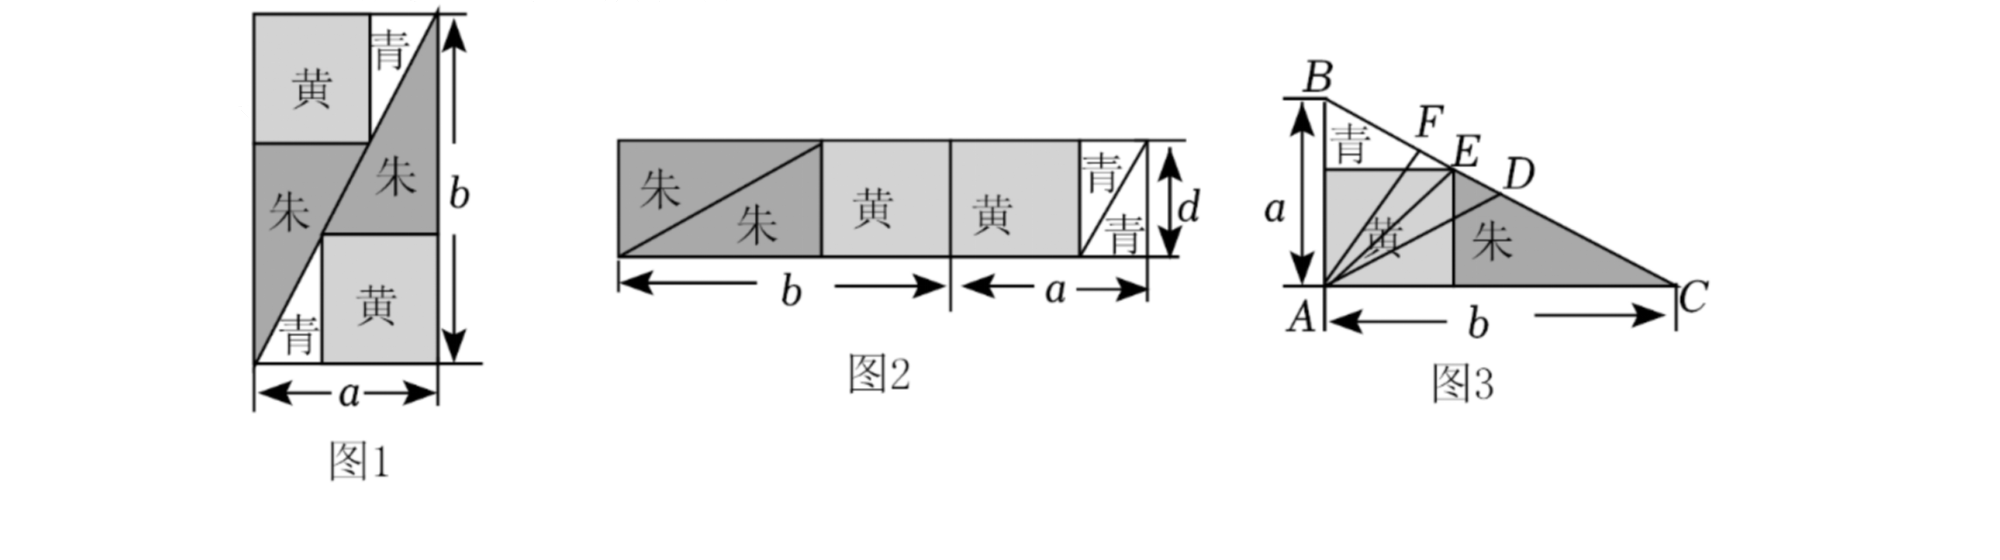
\includegraphics[width=0.86\textwidth]{figures/gao107_q11.png}
\end{center}

①由图 1 和图 2 面积相等得 $d=\dfrac{2ab}{a+b}$　　②由 $AE\geqslant AF$ 可得 $\sqrt{\dfrac{a^2+b^2}2}\geqslant\dfrac{a+b}2$

③由 $AD\geqslant AE$ 可得 $\sqrt{\dfrac{a^2+b^2}2}\geqslant\dfrac{2}{\dfrac1a+\dfrac1b}$　④由 $AD\geqslant AF$ 可得 $a^2+b^2\geqslant2ab$

\ifanswer
\solbegin
\step{对于①，由图 1 和图 2 面积相等得 $ab=(a+b)\times d$，所以 $d=\dfrac{ab}{a+b}$，故①错,}
\step{对于②，因为 $AF\perp BC$，所以 $\dfrac12ab=\dfrac12\sqrt{a^2+b^2}\times AF$,}
\step{所以 $AF=\dfrac{ab}{\sqrt{a^2+b^2}}$，$AE=\sqrt2d=\dfrac{\sqrt2ab}{a+b}$,}
\step{因为 $AE\geqslant AF$，所以 $\dfrac{\sqrt2ab}{a+b}\geqslant\dfrac{ab}{\sqrt{a^2+b^2}}$，整理得 $\sqrt{\dfrac{a^2+b^2}2}\geqslant\dfrac{a+b}2$，故②对,}
\step{对于③，因为 $D$ 是斜边 $BC$ 的中点，所以 $AD=\sqrt{\dfrac{a^2+b^2}2}$,}
\step{因为 $AD\geqslant AE$，所以 $\sqrt{\dfrac{a^2+b^2}2}\geqslant\dfrac{\sqrt2ab}{a+b}$，整理得 $\sqrt{\dfrac{a^2+b^2}2}\geqslant\dfrac{2}{\dfrac1a+\dfrac1b}$，故③对,}
\step{对于④，因为 $AD\geqslant AF$，所以 $\sqrt{\dfrac{a^2+b^2}2}\geqslant\dfrac{ab}{\sqrt{a^2+b^2}}$，整理得 $a^2+b^2\geqslant2ab$,}
\step{故④对,}
\step{故正确的是②③④.}
\solend
\fi

\item 设 $a,b,c,d\in\R$ 且$\lvert a-b\rvert\leqslant2$,$\lvert c-d\rvert\leqslant2$,$\lvert a\rvert\leqslant3$,$\lvert c\rvert\leqslant3$，则 $\lvert ad-bc\rvert$ 的最大值为\blankline[4.4em].% 原卷四处条件间均排半角逗号，照录

\ifanswer
\solbegin
\step{令 $a-b=e$,$c-d=f$，则 $\lvert e\rvert\leqslant2$,$\lvert f\rvert\leqslant2$,$\lvert a\rvert\leqslant3$,$\lvert c\rvert\leqslant3$}
\step{则 $\lvert ad-bc\rvert=\lvert a(c-f)-(a-e)c\rvert=\lvert ce-af\rvert\leqslant\lvert c\rvert\,\lvert e\rvert+\lvert a\rvert\,\lvert f\rvert\leqslant12$,}
\step{则 $\lvert ad-bc\rvert$ 的最大值为 12.}
\solend
\fi

\end{enumerate}

\bigsec{二、选择题}

\begin{enumerate}
\setcounter{enumi}{12}

\item 下列说法正确的是\mbox{（\quad）}

\keepwithprev
A. 若 $a>b>0$，则 $ac^2>bc^2$\qquad\qquad B. 若 $a<b<0$，则 $a^2>ab>b^2$

C. 若 $a>b$，则 $a^2>b^2$\qquad\qquad\qquad D. 若 $a<b$，则 $\dfrac1a>\dfrac1b$

\ifanswer
\solbegin
\step{$A$. 当 $a>b>0$ 时，取 $c=0$，则 $ac^2>bc^2$ 不成立，故 $A$ 错误；}
\step{$B$. 当 $a<b<0$ 时，由不等式的基本性质得 $a^2>ab>b^2>0$，故 $B$ 正确；}
\step{$C$. 当 $a>b$ 时，取 $a=0$，$b=-1$，则 $a^2>b^2$ 不成立，故 $C$ 错误；}
\step{$D$. 当 $a<b$ 时，取 $a=0$，$b=1$，则 $\dfrac1a>\dfrac1b$ 不成立，故 $D$ 错误.}
\step{故选 $B$.}
\solend
\fi

\item 小玲在学习《论语·子路》读到“其身正，不令而行；其身不正，虽令不从”，这句话的
数学含义可以理解为：“身正”是“令行”的\mbox{（\quad）}

\keepwithprev
A. 充分非必要条件\qquad\qquad B. 必要不充分条件

C. 充要条件\qquad\qquad\qquad D. 既非充分又非必要条件

\ifanswer
\solbegin
\step{其身正，不令而行，即身正$\Rightarrow$令行，所以“身正”是“令行”的充分条件；}
\step{又其身不正，虽令不从，即令行$\Rightarrow$身正，所以“身正”是“令行”的必要条件；}
\step{综上，“身正”是“令行”的充要条件. 故选 $C$.}
\solend
\fi

\item 某地对农户抽样调查，结果如下：电冰箱拥有率为 $45\%$，电视机拥有率为 $55\%$，洗衣
机拥有率为 $65\%$，拥有上述三种电器的任意两种的占 $35\%$，三种电器齐全的为 $25\%$，那
么一种电器也没有的农户所占比例是\mbox{（\quad）}

\keepwithprev
A. $12\%$\qquad B. $15\%$\qquad C. $18\%$\qquad D. $20\%$

\ifanswer
\solbegin
\step{设只有电冰箱和电视机的农户有 $a$ 家，只有电冰箱和洗衣机的农户有 $b$ 家,}
\step{只有洗衣机和电视机的农户有 $c$ 家,}
\step{只有电视机、电冰箱、洗衣机的分别有 $d$、$e$、$f$ 家,}
\step{没有任何电器的农户有 $x$ 家,}

\begin{center}
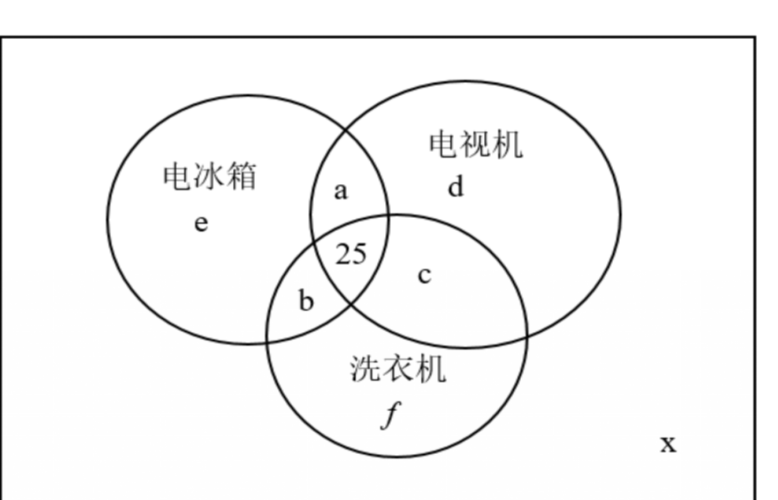
\includegraphics[width=0.42\textwidth]{figures/gao107_q15.png}
\end{center}

\step{所以 $25+a+b+e=45$①，$25+a+c+d=55$②,}
\step{$25+b+c+f=65$③,}
\step{把上面三个式子相加得 $2(a+b+c)+d+e+f=90$④,}
\step{对于拥有上述三种电器的任意两种的占 $35\%$，得 $a+b+c=35$⑤,}
\step{把⑤代入④可得到 $d+e+f=20$⑥,}
\step{因为农户共有 100 家，所以 $25+a+b+c+d+e+f+x=100$,}
\step{把⑤和⑥代入上式得 $x=20$，即一种电器也没有的农户所占比例为 $20\%$.}
\step{故选 $D$.}
\solend
\fi

\item 设 $d>0$，已知 $A,B$ 是两个数集. 若对任意 $x\in A$，都存在 $y\in B$，使得 $\lvert x-y\rvert<d$，则
称 $A$ 是 $B$ 的一个“$d-$邻集”. 现有下列两个命题：① $M=\{a+b\sqrt2\mid a,b\in\Z\}$ 是 $\Q$ 的一个
$\dfrac1{2025}$
一邻集；②若 $A$ 是 $B$ 的一个 $d-$邻集，则 $B$ 也是 $A$ 的一个 $d-$邻集；则\mbox{（\quad）}% 原卷把 d−邻集 的连字符断行后排成“一邻集”，照录

\keepwithprev
A. ①真②假\qquad B. ①假②真\qquad C. ①真②真\qquad D. ①假②假

\ifanswer
\solbegin
\step{对于①，任取 $M$ 中的元素 $x_0=a_0+b_0\sqrt2$,}
\step{则存在 $y_0\in\Q\cap\left(a_0+b_0\sqrt2-\dfrac1{2025},a_0+b_0\sqrt2+\dfrac1{2025}\right)$ 满足题意，故①正确；}
\step{对于②，取 $A=[-1,1]$,$B=[-2,2]$, $A$ 是 $B$ 的 $\dfrac12-$邻集，但反之不成立,}
\step{故②错误；}
\step{故选 $A$.}
\solend
\fi

\end{enumerate}

\bigsec{三、解答题}

\begin{enumerate}
\setcounter{enumi}{16}

\item 设 $a\in\R$，完成下列问题：

（1）求不等式 $3(a+1)x-3>2ax-3a$ 的解集 $M$；

（2）设集合 $A=\{x\mid x^2-ax+a^2-19=0\}$，$B=\{x\mid x^2-5x+6=0\}$，
$C=\{x\mid x^2+2x-8=0\}$. 若 $A\cap B\supset\varnothing$，$A\cap C=\varnothing$，求 $a$ 的值.

\ifanswer
\solbegin
\step{（1）不等式 $3(a+1)x-3>2ax-3a$ 可化为 $(a+3)x>3-3a$,}
\step{当 $a+3>0$，即 $a>-3$ 时，解得 $x>\dfrac{3-3a}{a+3}$,}
\step{当 $a+3=0$，即 $a=-3$ 时，不等式化为 $0\cdot x>12$，无解,}
\step{当 $a+3<0$，即 $a<-3$ 时，解得 $x<\dfrac{3-3a}{a+3}$,}
\step{综上所述，当 $a>-3$ 时，$M=\left(\dfrac{3-3a}{a+3},+\infty\right)$；}
\step{当 $a=-3$ 时，$M=\varnothing$；}
\step{当 $a<-3$ 时，$M=\left(-\infty,\dfrac{3-3a}{a+3}\right)$；}
\step{（2）$B=\{x\mid x^2-5x+6=0\}=\{2,3\}$，$C=\{x\mid x^2+2x-8=0\}=\{2,-4\}$,}
\step{因为 $A\cap B\supset\varnothing$，所以 $A\cap B\neq\varnothing$，又因为 $A\cap C=\varnothing$,}
\step{所以 $3\in A$，$2\notin A$，$-4\notin A$,}
\step{把 $x=3$ 代入方程 $x^2-ax+a^2-19=0$ 得 $9-3a+a^2-19=0$,}
\step{解得 $a=-2$ 或 $a=5$,}
\step{当 $a=-2$ 时，集合 $A=\{x\mid x^2+2x-15=0\}=\{3,-5\}$，符合题意,}
\step{当 $a=5$ 时，集合 $A=\{x\mid x^2-5x+6=0\}=\{3,2\}$，不符合题意，舍去,}
\step{综上所述，$a$ 的值为 $-2$.}
\solend
\fi

\item 完成下列问题：

（1）设 $x$、$y\in\R$，且 $x+y>5$，用反证法证明：$x>3$ 或 $y>2$；

（2）设 $x>0$，$a=x+1$，$b=\sqrt{x^2+7x+1}$，求 $\dfrac ba$ 的最大值.

\ifanswer
\solbegin
\step{（1）假设 $x\leqslant3$ 且 $y\leqslant2$，则 $x+y\leqslant3+2=5$，这与已知 $x+y>5$ 矛盾,}
\step{故 $x>3$ 或 $y>2$；}
\step{（2）$x>0$，$a=x+1$，$b=\sqrt{x^2+7x+1}$,}
\step{则 $\dfrac ba=\dfrac{\sqrt{x^2+7x+1}}{x+1}=\sqrt{\dfrac{x^2+7x+1}{x^2+2x+1}}=\sqrt{\dfrac{x^2+2x+1+5x}{x^2+2x+1}}$}
\step{$=\sqrt{1+\dfrac{5x}{x^2+2x+1}}=\sqrt{1+\dfrac{5}{x+\dfrac1x+2}}\leqslant\sqrt{1+\dfrac{5}{2\sqrt{x\cdot\dfrac1x}+2}}=\dfrac32$,}
\step{当且仅当 $x=\dfrac1x$，即 $x=1$ 时取等号，故 $\dfrac ba$ 的最大值为 $\dfrac32$.}
\solend
\fi

\item 已知函数 $f(x)=\lvert2x-a\rvert+a$.

（1）当 $a=2$ 时，求不等式 $f(x)\leqslant6+\lvert x+2\rvert$ 的解集；

（2）设 $g(x)=\lvert2x-1\rvert$，若不等式 $f(x)+g(x)\geqslant3$ 对一切 $x\in\R$ 恒成立，求实数 $a$ 的取值
范围.

\ifanswer
\solbegin
\ansspace*
\step{（1）$a=2$ 时，$f(x)=\lvert2x-2\rvert+2$,}
\step{则 $f(x)\leqslant6+\lvert x+2\rvert\Leftrightarrow\lvert2x-2\rvert+2\leqslant6+\lvert x+2\rvert$，即 $\lvert2x-2\rvert-\lvert x+2\rvert\leqslant4$,}
\step{当 $x<-2$ 时，$2-2x+x+2\leqslant4$，解得 $x\geqslant0$，与 $x<-2$ 取交集得 $\varnothing$,}
\step{当 $-2\leqslant x\leqslant1$ 时，$2-2x-x-2\leqslant4$，解得 $x\geqslant-\dfrac43$,}
\step{与 $-2\leqslant x\leqslant1$ 取交集得 $-\dfrac43\leqslant x\leqslant1$,}
\step{当 $x>1$ 时，$2x-2-x-2\leqslant4$，解得 $x\leqslant8$，与 $x>1$ 取交集得 $1<x\leqslant8$,}
\step{综上，不等式 $f(x)\leqslant6+\lvert x+2\rvert$ 的解集为 $\left\{x\,\middle|\,-\dfrac43\leqslant x\leqslant8\right\}$；}
\step{（2）$f(x)+g(x)\geqslant3$，即 $\lvert2x-a\rvert+a+\lvert2x-1\rvert\geqslant3$,}
\step{故 $\lvert2x-a\rvert+\lvert2x-1\rvert\geqslant3-a$,}
\step{当 $a\geqslant3$ 时，不等式显然成立,}
\step{当 $a<3$ 时,}
\step{由三角不等式得 $\lvert2x-a\rvert+\lvert2x-1\rvert\geqslant\lvert2x-a-(2x-1)\rvert=\lvert1-a\rvert$,}
\step{当且仅当 $(2x-a)(2x-1)\leqslant0$ 时取等号，因此 $\lvert1-a\rvert\geqslant3-a$,}
\step{平方得 $(1-a)^2\geqslant(3-a)^2$，解得 $a\geqslant2$，故 $2\leqslant a<3$.}
\step{综上，实数 $a$ 的取值范围是 $a\geqslant2$.}
\solend
\fi

\item 对于集合 $A,B$，定义集合 $A-B=\{x\mid x\in A$ 且 $x\notin B\}$.

（1）若 $A=\{1,2,3,4\}$,$B=\{3,4,5\}$，求集合 $A-B$ 和 $B-A$；

（2）给定集合 $A,B$，求所有满足方程组
\[
\begin{cases}
X\cap(A\cup B)=X\\
A\cap(B\cup X)=A\\
B\cap(A\cup X)=B\\
X\cap(A\cap B)=\varnothing
\end{cases}
\]
的集合 $X$（用 $A,B$ 表示）；

（3）用 $\lvert M\rvert$ 表示集合 $M$ 中的元素个数. 给定正整数 $n$，集合 $S=\{1,2,\cdots,n\}$. 对于实数
集的非空有限子集 $A,B$，定义集合 $C=\{x\mid x=a+b,a\in A,b\in B\}$. 求证：

$\lvert A-S\rvert+\lvert B-S\rvert+\lvert S-C\rvert\geqslant1$.

\ifanswer
\solbegin
\step{（1）由 $A=\{1,2,3,4\}$,$B=\{3,4,5\}$，则 $A-B=\{1,2\}$,$B-A=\{5\}$；}
\step{（2）由
$\begin{cases}
X\cap(A\cup B)=X\\
X\cap(A\cap B)=\varnothing
\end{cases}$，
得 $X\subseteq A-B$ 或 $X\subseteq B-A$,}
\step{再结合
$\begin{cases}
A\cap(B\cup X)=A\\
B\cap(A\cup X)=B
\end{cases}$，
得 $X=(A-B)\cup(B-A)$,}
\step{所以 $X=(A-B)\cup(B-A)$；}
\step{（3）$\lvert X\rvert$ 表示集合 $X$ 中的元素个数，则 $\lvert X\rvert\geqslant0$,}
\step{若 $A\cup B$ 中至少含有一个不在 $S$ 中的元素，则 $\lvert A-S\rvert+\lvert B-S\rvert\geqslant1$,}
\step{即 $\lvert A-S\rvert+\lvert B-S\rvert+\lvert S-C\rvert\geqslant1$.}
\step{若 $A\subseteq S$，且 $B\subseteq S$，则 $\lvert A-S\rvert=\lvert B-S\rvert=0$.}
\step{此时 $A$ 中最小的元素 $a\geqslant1$,$B$ 中最小的元素 $b\geqslant1$.}
\step{所以 $C$ 中最小的元素 $a+b\geqslant2$，则 $1\notin C$,}
\step{因为 $S=\{1,2,\cdots,n\}$，所以 $\lvert S-C\rvert\geqslant1$，即 $\lvert A-S\rvert+\lvert B-S\rvert+\lvert S-C\rvert\geqslant1$.}
\step{综上所述，$\lvert A-S\rvert+\lvert B-S\rvert+\lvert S-C\rvert\geqslant1$.}
\solend
\fi

\end{enumerate}

\end{document}
"
%
% 原始材料：微信公众号“魔都数学加油站”文章，作者破晓，2026-11-03 17:19 发布；
% 连载“27学年高一107”，原文标题“27学年高一107——2026-2027年上海市曹杨二中高一上10月月考”；
% 原文链接：https://mp.weixin.qq.com/s/IF4uB7aDNv-snYwbGMoDiQ。
% 正文为 10 张 PNG 页（第 1、2、4、6—9 页 4762×6735，第 3、5、10 页 2560×3620），题目下印有【解析】，为讲评版。
% 题目、解析均据原图转录；卷面水印及公众号页脚未录入。
% 第 11 题题干的三幅“出入相补”图（图 1—图 3）与第 15 题解析的三圆文氏图裁自原图、
% 去粉色水印转灰度（gao107_q11.png、gao107_q15.png），第 11 题图属题干（三版都出）、
% 第 15 题图属解析（仅答案版显示）。
%
% 卷首标题：原卷印作“2026-2027 年曹杨二中高一上 10 月月考”（公众号标题中的“上海市”
% 卷面标题行没有，本稿照卷面），年份区间按全稿惯例排 en dash；原卷未印副标题，本稿按题目内容
% 标为“集合与常用逻辑用语、不等式”。
%
% 与原卷的排版差异：
%   ① 原文从第 3 题起，填空题编号为 3—12、选择题为 13—16、解答题为 17—20，本稿保留原题号；
%   ② 原卷每题下直接印【解析】，本稿按全稿惯例将解析置于答案版；第 4 题只印【答案】另提 \ans{}；
%   ③ 原卷未印副标题，本稿按“知识模块”口径补出；
%   ④ 原卷填空横线按全稿惯例排为 \blankline[4.4em]；解答题按惯例加 \ansspace；选择题括号排
%      \mbox{（\quad）}、选项段前按惯例加 \keepwithprev；
%   ⑤ 原卷数集字母粗体与斜体混用（第 3 题 $\mathbf{R}$、第 4 题斜体 $R$、第 16 题粗体
%      $\mathbf{Z}$、$\mathbf{Q}$ 等），按全稿惯例统一改 \R、\Z、\Q。
%
% 原卷存疑：第 10 题解析“由 $\Delta=16m^2-8(2m^2+3m-2)\geqslant0$ 得 $m\leqslant\dfrac23$”
% 行末原卷无句读，照录。第 16 题解析②“取 $A=[-1,1]$，$B=[-2,2]$，$A$ 是 $B$ 的
% $\dfrac12$-邻集，但反之不成立”，据以判①真②假，照录。
%
% 行数核对：逐题数 \step/\stepm 条数，合计 112 条（Q3：5；Q4：0；Q5：2；Q6：2；Q7：2；
% Q8：4；Q9：8；Q10：4；Q11：9；Q12：3；Q13：5；Q14：3；Q15：12；Q16：5；Q17：15；
% Q18：6；Q19：15；Q20：12），与原卷印刷行逐题相等。第 4 题只印【答案】，提 \ans{}，
% 不计入 \step 账。
%
\documentclass[a4paper,11pt]{article}
\usepackage{common}

\begin{document}

\examtitlest[3]{2026--2027 年曹杨二中高一上 10 月月考}{集合与常用逻辑用语、不等式}

\bigsec{一、填空题}

\begin{enumerate}
\setcounter{enumi}{2}

\item 设 $a\in\R$，若 $3\in\{\sqrt3,a^2,a\}$，则 $a=$\blankline[4.4em].

\ifanswer
\solbegin
\step{因为 $3\in\{\sqrt3,a^2,a\}$，所以 $a^2=3$，解得 $a=\sqrt3$ 或 $a=-\sqrt3$,}
\step{当 $a=\sqrt3$ 时，集合为 $\{\sqrt3,3,\sqrt3\}$，不满足集合元素的互异性，舍去；}
\step{当 $a=-\sqrt3$ 时，集合为 $\{\sqrt3,3,-\sqrt3\}$，符合要求；}
\step{若 $a=3$，此时集合为 $\{\sqrt3,9,3\}$，符合要求；}
\step{综上，$a$ 为 $-\sqrt3$ 或 $3$.}
\solend
\fi

\item 设 $a\in\R$，已知集合 $A=\{x\mid x\leqslant a\}$，$B=\{x\mid x>2\}$. 若 $A\cup B=\R$，则 $a$ 的取值范围是\blankline[4.4em].

\ifanswer
\ans{$a\geqslant2$}
\fi

\item 设 $x>0$，$y>0$ 且 $x+3y=1$，则 $xy$ 的最大值为\blankline[4.4em].

\ifanswer
\solbegin
\step{由于 $x>0$，$y>0$ 且 $x+3y=1$，则 $1=x+3y\geqslant2\sqrt{3xy}$，得 $xy\leqslant\dfrac1{12}$,}
\step{当且仅当 $x=3y=\dfrac12$ 时取等号，则 $xy$ 的最大值为 $\dfrac1{12}$.}
\solend
\fi

\item 设 $a\in\R$，若集合$\left\{x\,\middle|\,\dfrac{ax}{x-1}=x\right\}$有且仅有两个子集，则 $a=$\blankline[4.4em].

\ifanswer
\solbegin
\step{由 $\dfrac{ax}{x-1}=x$ 得 $ax=x(x-1)$，即 $x(x-a-1)=0$,}
\step{所以此方程有两个相等的（不等于 1）的实数根或有一根为 1，所以 $a=-1$ 或 $0$.}
\solend
\fi

\item 已知全集 $U=\{x\mid x^2-8x-20<0\}$，集合 $A=\{x\mid 1-x^2>0$ 且 $x<0\}$，则 $\overline A=$\blankline[4.4em].

\ifanswer
\solbegin
\step{$U=\{x\mid-2<x<10\}$，$A=\{x\mid-1<x<0\}$,}
\step{所以 $\overline A=\{x\mid-2<x\leqslant-1$ 或 $0\leqslant x<10\}$.}
\solend
\fi

\item 设 $a,b\in\R$，若不等式 $-x^2-ax+b\geqslant0$ 的解集为 $[-2,3]$，则不等式 $\lvert ax+b\rvert<5$ 的解集为\blankline[4.4em].

\ifanswer
\solbegin
\step{由不等式 $-x^2-ax+b\geqslant0$ 的解集为 $[-2,3]$,}
\step{得 $-2$、$3$ 是方程 $-x^2-ax+b=0$ 的两个根，所以 $a=-1$，$b=6$.}
\step{解不等式 $\lvert-x+6\rvert<5$，得 $-5<x-6<5$，解得 $1<x<11$,}
\step{即所求不等式的解集为 $(1,11)$.}
\solend
\fi

\item 某货运卡车以 $x$ 千米／时的速度匀速行驶 300 千米，按交通法规限制 $50\leqslant x\leqslant100$，假设
柴油的价格为每升 6 元，汽车每小时耗油 $\left(4+\dfrac{x^2}{420}\right)$ 升，司机工资为每小时 46 元. 则当
$x=$\blankline[4.4em]（千米／时），这次行车的总费用（油费与司机工资的总和）最低.

\ifanswer
\solbegin
\step{因为卡车行驶 300 千米，速度为 $x$ 千米／时,}
\step{因此总用时为 $t=\dfrac{300}{x}$ 小时，其中 $50\leqslant x\leqslant100$,}
\step{每小时油费为 $6\cdot\left(4+\dfrac{x^2}{420}\right)$ 元，每小时司机工资为 46 元，因}
\step{此每小时总支出为 $6\cdot\left(4+\dfrac{x^2}{420}\right)+46=70+\dfrac{x^2}{70}$ 元.}
\step{设全程总费用为 $y$，则 $y=\dfrac{300}{x}\cdot\left(70+\dfrac{x^2}{70}\right)=\dfrac{21000}{x}+\dfrac{30x}{7}$,}
\step{因为 $50\leqslant x\leqslant100$，$\dfrac{21000}{x}+\dfrac{30x}{7}\geqslant2\sqrt{\dfrac{21000}{x}\cdot\dfrac{30x}{7}}=600$,}
\step{当且仅当 $\dfrac{21000}{x}=\dfrac{30x}{7}$，即 $x=70$ 时取等号，且 $70\in[50,100]$,}
\step{因此当 $x=70$ 千米／时，行车的总费用（油费与司机工资的总和）最低.}
\solend
\fi

\item 设 $x_1$、$x_2$ 是关于 $x$ 的方程 $2x^2-4mx+2m^2+3m-2=0$ 的两个实数根，则 $x_1^2+x_2^2$ 的最小值为\blankline[4.4em].

\ifanswer
\solbegin
\step{由题意得 $x_1+x_2=2m$，$x_1x_2=m^2+\dfrac{3m}{2}-1$,}
\step{由 $\Delta=16m^2-8(2m^2+3m-2)\geqslant0$ 得 $m\leqslant\dfrac23$}
\step{所以 $x_1^2+x_1^2=(x_1+x_2)^2-2x_1x_2=4m^2-2m^2+3m+2=2m^2-3m+2$,% 原卷左端作 x_1²+x_1²，照录
}
\step{结合二次函数的性质得，当 $m=\dfrac23$ 时取得最小值 $\dfrac89$.}
\solend
\fi

\item 小玲在钻研《九章算术》中“勾股容方”问题“今有勾五步，股十二步，问勾中容方几
何？”时，发现魏晋时期数学家刘徽在其《九章算术注》中利用出入相补原理给出了这个
问题的一般解法：如图 1，用对角线将长和宽分别为 $b$ 和 $a$ 的矩形分成两个直角三角形，
每个直角三角形再分成一个内接正方形（黄）和两个小直角三角形（朱、青）. 将三种颜色
的图形进行重组，得到如图 2 所示的矩形，该矩形长为 $a+b$，宽为内接正方形的边长
$d$. 由刘徽构造的图形可以得到许多重要的结论，如图 3，设 $D$ 为斜边 $BC$ 的中点，作直
角三角形 $ABC$ 的内接正方形对角线 $AE$，过点 $A$ 作 $AF\perp BC$ 于点 $F$，则下列四个推理中
正确的序号是\blankline[4.4em].

\begin{center}
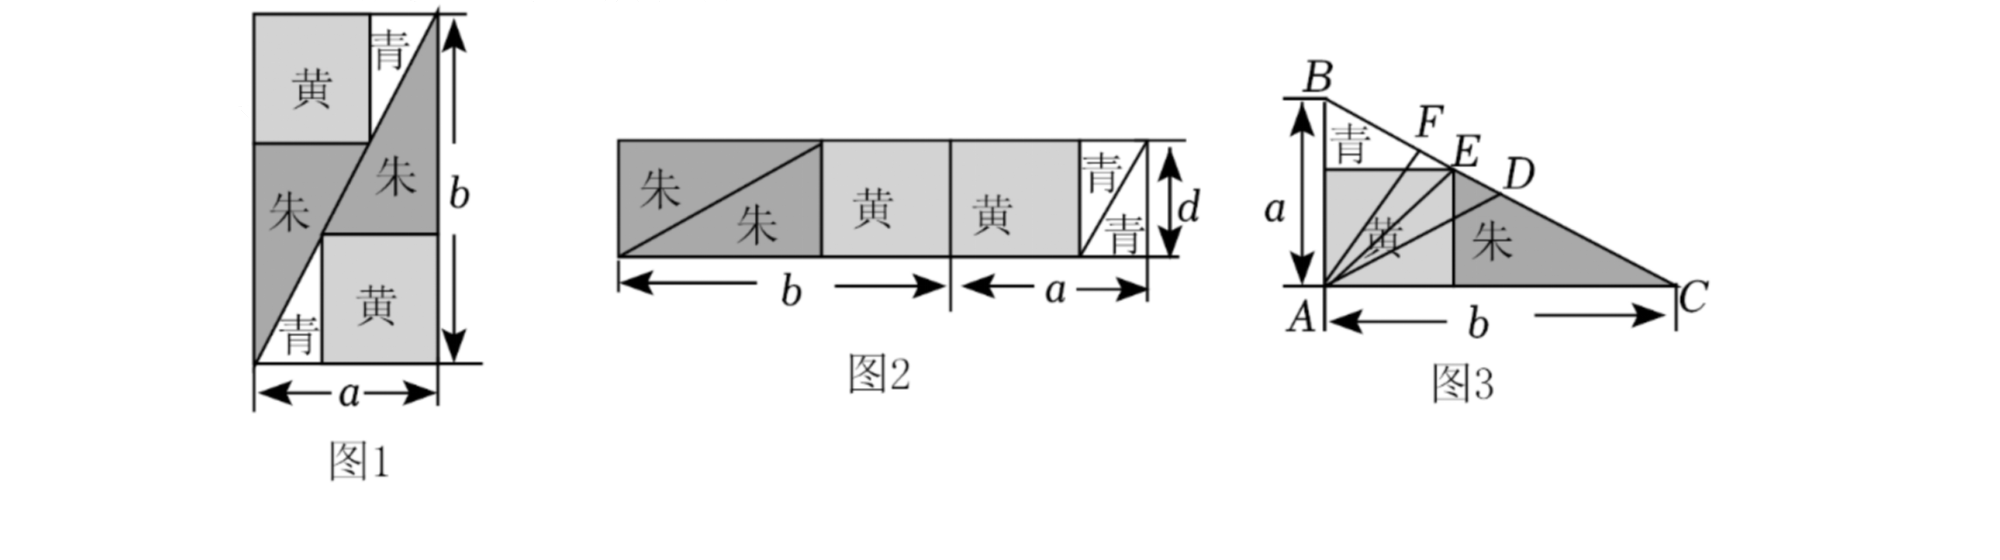
\includegraphics[width=0.86\textwidth]{figures/gao107_q11.png}
\end{center}

①由图 1 和图 2 面积相等得 $d=\dfrac{2ab}{a+b}$　　②由 $AE\geqslant AF$ 可得 $\sqrt{\dfrac{a^2+b^2}2}\geqslant\dfrac{a+b}2$

③由 $AD\geqslant AE$ 可得 $\sqrt{\dfrac{a^2+b^2}2}\geqslant\dfrac{2}{\dfrac1a+\dfrac1b}$　④由 $AD\geqslant AF$ 可得 $a^2+b^2\geqslant2ab$

\ifanswer
\solbegin
\step{对于①，由图 1 和图 2 面积相等得 $ab=(a+b)\times d$，所以 $d=\dfrac{ab}{a+b}$，故①错,}
\step{对于②，因为 $AF\perp BC$，所以 $\dfrac12ab=\dfrac12\sqrt{a^2+b^2}\times AF$,}
\step{所以 $AF=\dfrac{ab}{\sqrt{a^2+b^2}}$，$AE=\sqrt2d=\dfrac{\sqrt2ab}{a+b}$,}
\step{因为 $AE\geqslant AF$，所以 $\dfrac{\sqrt2ab}{a+b}\geqslant\dfrac{ab}{\sqrt{a^2+b^2}}$，整理得 $\sqrt{\dfrac{a^2+b^2}2}\geqslant\dfrac{a+b}2$，故②对,}
\step{对于③，因为 $D$ 是斜边 $BC$ 的中点，所以 $AD=\sqrt{\dfrac{a^2+b^2}2}$,}
\step{因为 $AD\geqslant AE$，所以 $\sqrt{\dfrac{a^2+b^2}2}\geqslant\dfrac{\sqrt2ab}{a+b}$，整理得 $\sqrt{\dfrac{a^2+b^2}2}\geqslant\dfrac{2}{\dfrac1a+\dfrac1b}$，故③对,}
\step{对于④，因为 $AD\geqslant AF$，所以 $\sqrt{\dfrac{a^2+b^2}2}\geqslant\dfrac{ab}{\sqrt{a^2+b^2}}$，整理得 $a^2+b^2\geqslant2ab$,}
\step{故④对,}
\step{故正确的是②③④.}
\solend
\fi

\item 设 $a,b,c,d\in\R$ 且$\lvert a-b\rvert\leqslant2$,$\lvert c-d\rvert\leqslant2$,$\lvert a\rvert\leqslant3$,$\lvert c\rvert\leqslant3$，则 $\lvert ad-bc\rvert$ 的最大值为\blankline[4.4em].% 原卷四处条件间均排半角逗号，照录

\ifanswer
\solbegin
\step{令 $a-b=e$,$c-d=f$，则 $\lvert e\rvert\leqslant2$,$\lvert f\rvert\leqslant2$,$\lvert a\rvert\leqslant3$,$\lvert c\rvert\leqslant3$}
\step{则 $\lvert ad-bc\rvert=\lvert a(c-f)-(a-e)c\rvert=\lvert ce-af\rvert\leqslant\lvert c\rvert\,\lvert e\rvert+\lvert a\rvert\,\lvert f\rvert\leqslant12$,}
\step{则 $\lvert ad-bc\rvert$ 的最大值为 12.}
\solend
\fi

\end{enumerate}

\bigsec{二、选择题}

\begin{enumerate}
\setcounter{enumi}{12}

\item 下列说法正确的是\mbox{（\quad）}

\keepwithprev
A. 若 $a>b>0$，则 $ac^2>bc^2$\qquad\qquad B. 若 $a<b<0$，则 $a^2>ab>b^2$

C. 若 $a>b$，则 $a^2>b^2$\qquad\qquad\qquad D. 若 $a<b$，则 $\dfrac1a>\dfrac1b$

\ifanswer
\solbegin
\step{$A$. 当 $a>b>0$ 时，取 $c=0$，则 $ac^2>bc^2$ 不成立，故 $A$ 错误；}
\step{$B$. 当 $a<b<0$ 时，由不等式的基本性质得 $a^2>ab>b^2>0$，故 $B$ 正确；}
\step{$C$. 当 $a>b$ 时，取 $a=0$，$b=-1$，则 $a^2>b^2$ 不成立，故 $C$ 错误；}
\step{$D$. 当 $a<b$ 时，取 $a=0$，$b=1$，则 $\dfrac1a>\dfrac1b$ 不成立，故 $D$ 错误.}
\step{故选 $B$.}
\solend
\fi

\item 小玲在学习《论语·子路》读到“其身正，不令而行；其身不正，虽令不从”，这句话的
数学含义可以理解为：“身正”是“令行”的\mbox{（\quad）}

\keepwithprev
A. 充分非必要条件\qquad\qquad B. 必要不充分条件

C. 充要条件\qquad\qquad\qquad D. 既非充分又非必要条件

\ifanswer
\solbegin
\step{其身正，不令而行，即身正$\Rightarrow$令行，所以“身正”是“令行”的充分条件；}
\step{又其身不正，虽令不从，即令行$\Rightarrow$身正，所以“身正”是“令行”的必要条件；}
\step{综上，“身正”是“令行”的充要条件. 故选 $C$.}
\solend
\fi

\item 某地对农户抽样调查，结果如下：电冰箱拥有率为 $45\%$，电视机拥有率为 $55\%$，洗衣
机拥有率为 $65\%$，拥有上述三种电器的任意两种的占 $35\%$，三种电器齐全的为 $25\%$，那
么一种电器也没有的农户所占比例是\mbox{（\quad）}

\keepwithprev
A. $12\%$\qquad B. $15\%$\qquad C. $18\%$\qquad D. $20\%$

\ifanswer
\solbegin
\step{设只有电冰箱和电视机的农户有 $a$ 家，只有电冰箱和洗衣机的农户有 $b$ 家,}
\step{只有洗衣机和电视机的农户有 $c$ 家,}
\step{只有电视机、电冰箱、洗衣机的分别有 $d$、$e$、$f$ 家,}
\step{没有任何电器的农户有 $x$ 家,}

\begin{center}
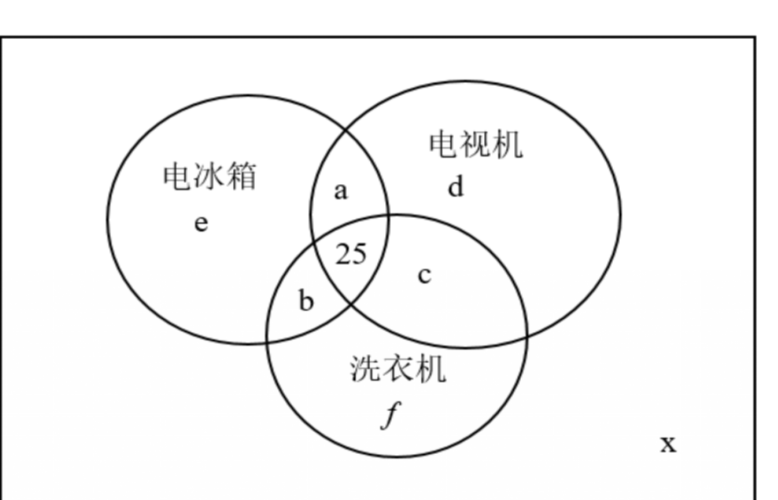
\includegraphics[width=0.42\textwidth]{figures/gao107_q15.png}
\end{center}

\step{所以 $25+a+b+e=45$①，$25+a+c+d=55$②,}
\step{$25+b+c+f=65$③,}
\step{把上面三个式子相加得 $2(a+b+c)+d+e+f=90$④,}
\step{对于拥有上述三种电器的任意两种的占 $35\%$，得 $a+b+c=35$⑤,}
\step{把⑤代入④可得到 $d+e+f=20$⑥,}
\step{因为农户共有 100 家，所以 $25+a+b+c+d+e+f+x=100$,}
\step{把⑤和⑥代入上式得 $x=20$，即一种电器也没有的农户所占比例为 $20\%$.}
\step{故选 $D$.}
\solend
\fi

\item 设 $d>0$，已知 $A,B$ 是两个数集. 若对任意 $x\in A$，都存在 $y\in B$，使得 $\lvert x-y\rvert<d$，则
称 $A$ 是 $B$ 的一个“$d-$邻集”. 现有下列两个命题：① $M=\{a+b\sqrt2\mid a,b\in\Z\}$ 是 $\Q$ 的一个
$\dfrac1{2025}$
一邻集；②若 $A$ 是 $B$ 的一个 $d-$邻集，则 $B$ 也是 $A$ 的一个 $d-$邻集；则\mbox{（\quad）}% 原卷把 d−邻集 的连字符断行后排成“一邻集”，照录

\keepwithprev
A. ①真②假\qquad B. ①假②真\qquad C. ①真②真\qquad D. ①假②假

\ifanswer
\solbegin
\step{对于①，任取 $M$ 中的元素 $x_0=a_0+b_0\sqrt2$,}
\step{则存在 $y_0\in\Q\cap\left(a_0+b_0\sqrt2-\dfrac1{2025},a_0+b_0\sqrt2+\dfrac1{2025}\right)$ 满足题意，故①正确；}
\step{对于②，取 $A=[-1,1]$,$B=[-2,2]$, $A$ 是 $B$ 的 $\dfrac12-$邻集，但反之不成立,}
\step{故②错误；}
\step{故选 $A$.}
\solend
\fi

\end{enumerate}

\bigsec{三、解答题}

\begin{enumerate}
\setcounter{enumi}{16}

\item 设 $a\in\R$，完成下列问题：

（1）求不等式 $3(a+1)x-3>2ax-3a$ 的解集 $M$；

（2）设集合 $A=\{x\mid x^2-ax+a^2-19=0\}$，$B=\{x\mid x^2-5x+6=0\}$，
$C=\{x\mid x^2+2x-8=0\}$. 若 $A\cap B\supset\varnothing$，$A\cap C=\varnothing$，求 $a$ 的值.

\ifanswer
\solbegin
\step{（1）不等式 $3(a+1)x-3>2ax-3a$ 可化为 $(a+3)x>3-3a$,}
\step{当 $a+3>0$，即 $a>-3$ 时，解得 $x>\dfrac{3-3a}{a+3}$,}
\step{当 $a+3=0$，即 $a=-3$ 时，不等式化为 $0\cdot x>12$，无解,}
\step{当 $a+3<0$，即 $a<-3$ 时，解得 $x<\dfrac{3-3a}{a+3}$,}
\step{综上所述，当 $a>-3$ 时，$M=\left(\dfrac{3-3a}{a+3},+\infty\right)$；}
\step{当 $a=-3$ 时，$M=\varnothing$；}
\step{当 $a<-3$ 时，$M=\left(-\infty,\dfrac{3-3a}{a+3}\right)$；}
\step{（2）$B=\{x\mid x^2-5x+6=0\}=\{2,3\}$，$C=\{x\mid x^2+2x-8=0\}=\{2,-4\}$,}
\step{因为 $A\cap B\supset\varnothing$，所以 $A\cap B\neq\varnothing$，又因为 $A\cap C=\varnothing$,}
\step{所以 $3\in A$，$2\notin A$，$-4\notin A$,}
\step{把 $x=3$ 代入方程 $x^2-ax+a^2-19=0$ 得 $9-3a+a^2-19=0$,}
\step{解得 $a=-2$ 或 $a=5$,}
\step{当 $a=-2$ 时，集合 $A=\{x\mid x^2+2x-15=0\}=\{3,-5\}$，符合题意,}
\step{当 $a=5$ 时，集合 $A=\{x\mid x^2-5x+6=0\}=\{3,2\}$，不符合题意，舍去,}
\step{综上所述，$a$ 的值为 $-2$.}
\solend
\fi

\item 完成下列问题：

（1）设 $x$、$y\in\R$，且 $x+y>5$，用反证法证明：$x>3$ 或 $y>2$；

（2）设 $x>0$，$a=x+1$，$b=\sqrt{x^2+7x+1}$，求 $\dfrac ba$ 的最大值.

\ifanswer
\solbegin
\step{（1）假设 $x\leqslant3$ 且 $y\leqslant2$，则 $x+y\leqslant3+2=5$，这与已知 $x+y>5$ 矛盾,}
\step{故 $x>3$ 或 $y>2$；}
\step{（2）$x>0$，$a=x+1$，$b=\sqrt{x^2+7x+1}$,}
\step{则 $\dfrac ba=\dfrac{\sqrt{x^2+7x+1}}{x+1}=\sqrt{\dfrac{x^2+7x+1}{x^2+2x+1}}=\sqrt{\dfrac{x^2+2x+1+5x}{x^2+2x+1}}$}
\step{$=\sqrt{1+\dfrac{5x}{x^2+2x+1}}=\sqrt{1+\dfrac{5}{x+\dfrac1x+2}}\leqslant\sqrt{1+\dfrac{5}{2\sqrt{x\cdot\dfrac1x}+2}}=\dfrac32$,}
\step{当且仅当 $x=\dfrac1x$，即 $x=1$ 时取等号，故 $\dfrac ba$ 的最大值为 $\dfrac32$.}
\solend
\fi

\item 已知函数 $f(x)=\lvert2x-a\rvert+a$.

（1）当 $a=2$ 时，求不等式 $f(x)\leqslant6+\lvert x+2\rvert$ 的解集；

（2）设 $g(x)=\lvert2x-1\rvert$，若不等式 $f(x)+g(x)\geqslant3$ 对一切 $x\in\R$ 恒成立，求实数 $a$ 的取值
范围.

\ifanswer
\solbegin
\ansspace*
\step{（1）$a=2$ 时，$f(x)=\lvert2x-2\rvert+2$,}
\step{则 $f(x)\leqslant6+\lvert x+2\rvert\Leftrightarrow\lvert2x-2\rvert+2\leqslant6+\lvert x+2\rvert$，即 $\lvert2x-2\rvert-\lvert x+2\rvert\leqslant4$,}
\step{当 $x<-2$ 时，$2-2x+x+2\leqslant4$，解得 $x\geqslant0$，与 $x<-2$ 取交集得 $\varnothing$,}
\step{当 $-2\leqslant x\leqslant1$ 时，$2-2x-x-2\leqslant4$，解得 $x\geqslant-\dfrac43$,}
\step{与 $-2\leqslant x\leqslant1$ 取交集得 $-\dfrac43\leqslant x\leqslant1$,}
\step{当 $x>1$ 时，$2x-2-x-2\leqslant4$，解得 $x\leqslant8$，与 $x>1$ 取交集得 $1<x\leqslant8$,}
\step{综上，不等式 $f(x)\leqslant6+\lvert x+2\rvert$ 的解集为 $\left\{x\,\middle|\,-\dfrac43\leqslant x\leqslant8\right\}$；}
\step{（2）$f(x)+g(x)\geqslant3$，即 $\lvert2x-a\rvert+a+\lvert2x-1\rvert\geqslant3$,}
\step{故 $\lvert2x-a\rvert+\lvert2x-1\rvert\geqslant3-a$,}
\step{当 $a\geqslant3$ 时，不等式显然成立,}
\step{当 $a<3$ 时,}
\step{由三角不等式得 $\lvert2x-a\rvert+\lvert2x-1\rvert\geqslant\lvert2x-a-(2x-1)\rvert=\lvert1-a\rvert$,}
\step{当且仅当 $(2x-a)(2x-1)\leqslant0$ 时取等号，因此 $\lvert1-a\rvert\geqslant3-a$,}
\step{平方得 $(1-a)^2\geqslant(3-a)^2$，解得 $a\geqslant2$，故 $2\leqslant a<3$.}
\step{综上，实数 $a$ 的取值范围是 $a\geqslant2$.}
\solend
\fi

\item 对于集合 $A,B$，定义集合 $A-B=\{x\mid x\in A$ 且 $x\notin B\}$.

（1）若 $A=\{1,2,3,4\}$,$B=\{3,4,5\}$，求集合 $A-B$ 和 $B-A$；

（2）给定集合 $A,B$，求所有满足方程组
\[
\begin{cases}
X\cap(A\cup B)=X\\
A\cap(B\cup X)=A\\
B\cap(A\cup X)=B\\
X\cap(A\cap B)=\varnothing
\end{cases}
\]
的集合 $X$（用 $A,B$ 表示）；

（3）用 $\lvert M\rvert$ 表示集合 $M$ 中的元素个数. 给定正整数 $n$，集合 $S=\{1,2,\cdots,n\}$. 对于实数
集的非空有限子集 $A,B$，定义集合 $C=\{x\mid x=a+b,a\in A,b\in B\}$. 求证：

$\lvert A-S\rvert+\lvert B-S\rvert+\lvert S-C\rvert\geqslant1$.

\ifanswer
\solbegin
\step{（1）由 $A=\{1,2,3,4\}$,$B=\{3,4,5\}$，则 $A-B=\{1,2\}$,$B-A=\{5\}$；}
\step{（2）由
$\begin{cases}
X\cap(A\cup B)=X\\
X\cap(A\cap B)=\varnothing
\end{cases}$，
得 $X\subseteq A-B$ 或 $X\subseteq B-A$,}
\step{再结合
$\begin{cases}
A\cap(B\cup X)=A\\
B\cap(A\cup X)=B
\end{cases}$，
得 $X=(A-B)\cup(B-A)$,}
\step{所以 $X=(A-B)\cup(B-A)$；}
\step{（3）$\lvert X\rvert$ 表示集合 $X$ 中的元素个数，则 $\lvert X\rvert\geqslant0$,}
\step{若 $A\cup B$ 中至少含有一个不在 $S$ 中的元素，则 $\lvert A-S\rvert+\lvert B-S\rvert\geqslant1$,}
\step{即 $\lvert A-S\rvert+\lvert B-S\rvert+\lvert S-C\rvert\geqslant1$.}
\step{若 $A\subseteq S$，且 $B\subseteq S$，则 $\lvert A-S\rvert=\lvert B-S\rvert=0$.}
\step{此时 $A$ 中最小的元素 $a\geqslant1$,$B$ 中最小的元素 $b\geqslant1$.}
\step{所以 $C$ 中最小的元素 $a+b\geqslant2$，则 $1\notin C$,}
\step{因为 $S=\{1,2,\cdots,n\}$，所以 $\lvert S-C\rvert\geqslant1$，即 $\lvert A-S\rvert+\lvert B-S\rvert+\lvert S-C\rvert\geqslant1$.}
\step{综上所述，$\lvert A-S\rvert+\lvert B-S\rvert+\lvert S-C\rvert\geqslant1$.}
\solend
\fi

\end{enumerate}

\end{document}
"
% 紧凑版：xelatex "\def\iscompact{1}% 高一107_曹杨二中_10月月考.tex
%   —— 高一上数学“2026-2027 年曹杨二中高一上 10 月月考”（试卷版/答案版）
% 试卷版：xelatex 高一107_曹杨二中_10月月考.tex
% 答案版：xelatex "\def\isanswer{1}% 高一107_曹杨二中_10月月考.tex
%   —— 高一上数学“2026-2027 年曹杨二中高一上 10 月月考”（试卷版/答案版）
% 试卷版：xelatex 高一107_曹杨二中_10月月考.tex
% 答案版：xelatex "\def\isanswer{1}% 高一107_曹杨二中_10月月考.tex
%   —— 高一上数学“2026-2027 年曹杨二中高一上 10 月月考”（试卷版/答案版）
% 试卷版：xelatex 高一107_曹杨二中_10月月考.tex
% 答案版：xelatex "\def\isanswer{1}\input{高一107_曹杨二中_10月月考.tex}"
% 紧凑版：xelatex "\def\iscompact{1}\input{高一107_曹杨二中_10月月考.tex}"
%
% 原始材料：微信公众号“魔都数学加油站”文章，作者破晓，2026-11-03 17:19 发布；
% 连载“27学年高一107”，原文标题“27学年高一107——2026-2027年上海市曹杨二中高一上10月月考”；
% 原文链接：https://mp.weixin.qq.com/s/IF4uB7aDNv-snYwbGMoDiQ。
% 正文为 10 张 PNG 页（第 1、2、4、6—9 页 4762×6735，第 3、5、10 页 2560×3620），题目下印有【解析】，为讲评版。
% 题目、解析均据原图转录；卷面水印及公众号页脚未录入。
% 第 11 题题干的三幅“出入相补”图（图 1—图 3）与第 15 题解析的三圆文氏图裁自原图、
% 去粉色水印转灰度（gao107_q11.png、gao107_q15.png），第 11 题图属题干（三版都出）、
% 第 15 题图属解析（仅答案版显示）。
%
% 卷首标题：原卷印作“2026-2027 年曹杨二中高一上 10 月月考”（公众号标题中的“上海市”
% 卷面标题行没有，本稿照卷面），年份区间按全稿惯例排 en dash；原卷未印副标题，本稿按题目内容
% 标为“集合与常用逻辑用语、不等式”。
%
% 与原卷的排版差异：
%   ① 原文从第 3 题起，填空题编号为 3—12、选择题为 13—16、解答题为 17—20，本稿保留原题号；
%   ② 原卷每题下直接印【解析】，本稿按全稿惯例将解析置于答案版；第 4 题只印【答案】另提 \ans{}；
%   ③ 原卷未印副标题，本稿按“知识模块”口径补出；
%   ④ 原卷填空横线按全稿惯例排为 \blankline[4.4em]；解答题按惯例加 \ansspace；选择题括号排
%      \mbox{（\quad）}、选项段前按惯例加 \keepwithprev；
%   ⑤ 原卷数集字母粗体与斜体混用（第 3 题 $\mathbf{R}$、第 4 题斜体 $R$、第 16 题粗体
%      $\mathbf{Z}$、$\mathbf{Q}$ 等），按全稿惯例统一改 \R、\Z、\Q。
%
% 原卷存疑：第 10 题解析“由 $\Delta=16m^2-8(2m^2+3m-2)\geqslant0$ 得 $m\leqslant\dfrac23$”
% 行末原卷无句读，照录。第 16 题解析②“取 $A=[-1,1]$，$B=[-2,2]$，$A$ 是 $B$ 的
% $\dfrac12$-邻集，但反之不成立”，据以判①真②假，照录。
%
% 行数核对：逐题数 \step/\stepm 条数，合计 112 条（Q3：5；Q4：0；Q5：2；Q6：2；Q7：2；
% Q8：4；Q9：8；Q10：4；Q11：9；Q12：3；Q13：5；Q14：3；Q15：12；Q16：5；Q17：15；
% Q18：6；Q19：15；Q20：12），与原卷印刷行逐题相等。第 4 题只印【答案】，提 \ans{}，
% 不计入 \step 账。
%
\documentclass[a4paper,11pt]{article}
\usepackage{common}

\begin{document}

\examtitlest[3]{2026--2027 年曹杨二中高一上 10 月月考}{集合与常用逻辑用语、不等式}

\bigsec{一、填空题}

\begin{enumerate}
\setcounter{enumi}{2}

\item 设 $a\in\R$，若 $3\in\{\sqrt3,a^2,a\}$，则 $a=$\blankline[4.4em].

\ifanswer
\solbegin
\step{因为 $3\in\{\sqrt3,a^2,a\}$，所以 $a^2=3$，解得 $a=\sqrt3$ 或 $a=-\sqrt3$,}
\step{当 $a=\sqrt3$ 时，集合为 $\{\sqrt3,3,\sqrt3\}$，不满足集合元素的互异性，舍去；}
\step{当 $a=-\sqrt3$ 时，集合为 $\{\sqrt3,3,-\sqrt3\}$，符合要求；}
\step{若 $a=3$，此时集合为 $\{\sqrt3,9,3\}$，符合要求；}
\step{综上，$a$ 为 $-\sqrt3$ 或 $3$.}
\solend
\fi

\item 设 $a\in\R$，已知集合 $A=\{x\mid x\leqslant a\}$，$B=\{x\mid x>2\}$. 若 $A\cup B=\R$，则 $a$ 的取值范围是\blankline[4.4em].

\ifanswer
\ans{$a\geqslant2$}
\fi

\item 设 $x>0$，$y>0$ 且 $x+3y=1$，则 $xy$ 的最大值为\blankline[4.4em].

\ifanswer
\solbegin
\step{由于 $x>0$，$y>0$ 且 $x+3y=1$，则 $1=x+3y\geqslant2\sqrt{3xy}$，得 $xy\leqslant\dfrac1{12}$,}
\step{当且仅当 $x=3y=\dfrac12$ 时取等号，则 $xy$ 的最大值为 $\dfrac1{12}$.}
\solend
\fi

\item 设 $a\in\R$，若集合$\left\{x\,\middle|\,\dfrac{ax}{x-1}=x\right\}$有且仅有两个子集，则 $a=$\blankline[4.4em].

\ifanswer
\solbegin
\step{由 $\dfrac{ax}{x-1}=x$ 得 $ax=x(x-1)$，即 $x(x-a-1)=0$,}
\step{所以此方程有两个相等的（不等于 1）的实数根或有一根为 1，所以 $a=-1$ 或 $0$.}
\solend
\fi

\item 已知全集 $U=\{x\mid x^2-8x-20<0\}$，集合 $A=\{x\mid 1-x^2>0$ 且 $x<0\}$，则 $\overline A=$\blankline[4.4em].

\ifanswer
\solbegin
\step{$U=\{x\mid-2<x<10\}$，$A=\{x\mid-1<x<0\}$,}
\step{所以 $\overline A=\{x\mid-2<x\leqslant-1$ 或 $0\leqslant x<10\}$.}
\solend
\fi

\item 设 $a,b\in\R$，若不等式 $-x^2-ax+b\geqslant0$ 的解集为 $[-2,3]$，则不等式 $\lvert ax+b\rvert<5$ 的解集为\blankline[4.4em].

\ifanswer
\solbegin
\step{由不等式 $-x^2-ax+b\geqslant0$ 的解集为 $[-2,3]$,}
\step{得 $-2$、$3$ 是方程 $-x^2-ax+b=0$ 的两个根，所以 $a=-1$，$b=6$.}
\step{解不等式 $\lvert-x+6\rvert<5$，得 $-5<x-6<5$，解得 $1<x<11$,}
\step{即所求不等式的解集为 $(1,11)$.}
\solend
\fi

\item 某货运卡车以 $x$ 千米／时的速度匀速行驶 300 千米，按交通法规限制 $50\leqslant x\leqslant100$，假设
柴油的价格为每升 6 元，汽车每小时耗油 $\left(4+\dfrac{x^2}{420}\right)$ 升，司机工资为每小时 46 元. 则当
$x=$\blankline[4.4em]（千米／时），这次行车的总费用（油费与司机工资的总和）最低.

\ifanswer
\solbegin
\step{因为卡车行驶 300 千米，速度为 $x$ 千米／时,}
\step{因此总用时为 $t=\dfrac{300}{x}$ 小时，其中 $50\leqslant x\leqslant100$,}
\step{每小时油费为 $6\cdot\left(4+\dfrac{x^2}{420}\right)$ 元，每小时司机工资为 46 元，因}
\step{此每小时总支出为 $6\cdot\left(4+\dfrac{x^2}{420}\right)+46=70+\dfrac{x^2}{70}$ 元.}
\step{设全程总费用为 $y$，则 $y=\dfrac{300}{x}\cdot\left(70+\dfrac{x^2}{70}\right)=\dfrac{21000}{x}+\dfrac{30x}{7}$,}
\step{因为 $50\leqslant x\leqslant100$，$\dfrac{21000}{x}+\dfrac{30x}{7}\geqslant2\sqrt{\dfrac{21000}{x}\cdot\dfrac{30x}{7}}=600$,}
\step{当且仅当 $\dfrac{21000}{x}=\dfrac{30x}{7}$，即 $x=70$ 时取等号，且 $70\in[50,100]$,}
\step{因此当 $x=70$ 千米／时，行车的总费用（油费与司机工资的总和）最低.}
\solend
\fi

\item 设 $x_1$、$x_2$ 是关于 $x$ 的方程 $2x^2-4mx+2m^2+3m-2=0$ 的两个实数根，则 $x_1^2+x_2^2$ 的最小值为\blankline[4.4em].

\ifanswer
\solbegin
\step{由题意得 $x_1+x_2=2m$，$x_1x_2=m^2+\dfrac{3m}{2}-1$,}
\step{由 $\Delta=16m^2-8(2m^2+3m-2)\geqslant0$ 得 $m\leqslant\dfrac23$}
\step{所以 $x_1^2+x_1^2=(x_1+x_2)^2-2x_1x_2=4m^2-2m^2+3m+2=2m^2-3m+2$,% 原卷左端作 x_1²+x_1²，照录
}
\step{结合二次函数的性质得，当 $m=\dfrac23$ 时取得最小值 $\dfrac89$.}
\solend
\fi

\item 小玲在钻研《九章算术》中“勾股容方”问题“今有勾五步，股十二步，问勾中容方几
何？”时，发现魏晋时期数学家刘徽在其《九章算术注》中利用出入相补原理给出了这个
问题的一般解法：如图 1，用对角线将长和宽分别为 $b$ 和 $a$ 的矩形分成两个直角三角形，
每个直角三角形再分成一个内接正方形（黄）和两个小直角三角形（朱、青）. 将三种颜色
的图形进行重组，得到如图 2 所示的矩形，该矩形长为 $a+b$，宽为内接正方形的边长
$d$. 由刘徽构造的图形可以得到许多重要的结论，如图 3，设 $D$ 为斜边 $BC$ 的中点，作直
角三角形 $ABC$ 的内接正方形对角线 $AE$，过点 $A$ 作 $AF\perp BC$ 于点 $F$，则下列四个推理中
正确的序号是\blankline[4.4em].

\begin{center}
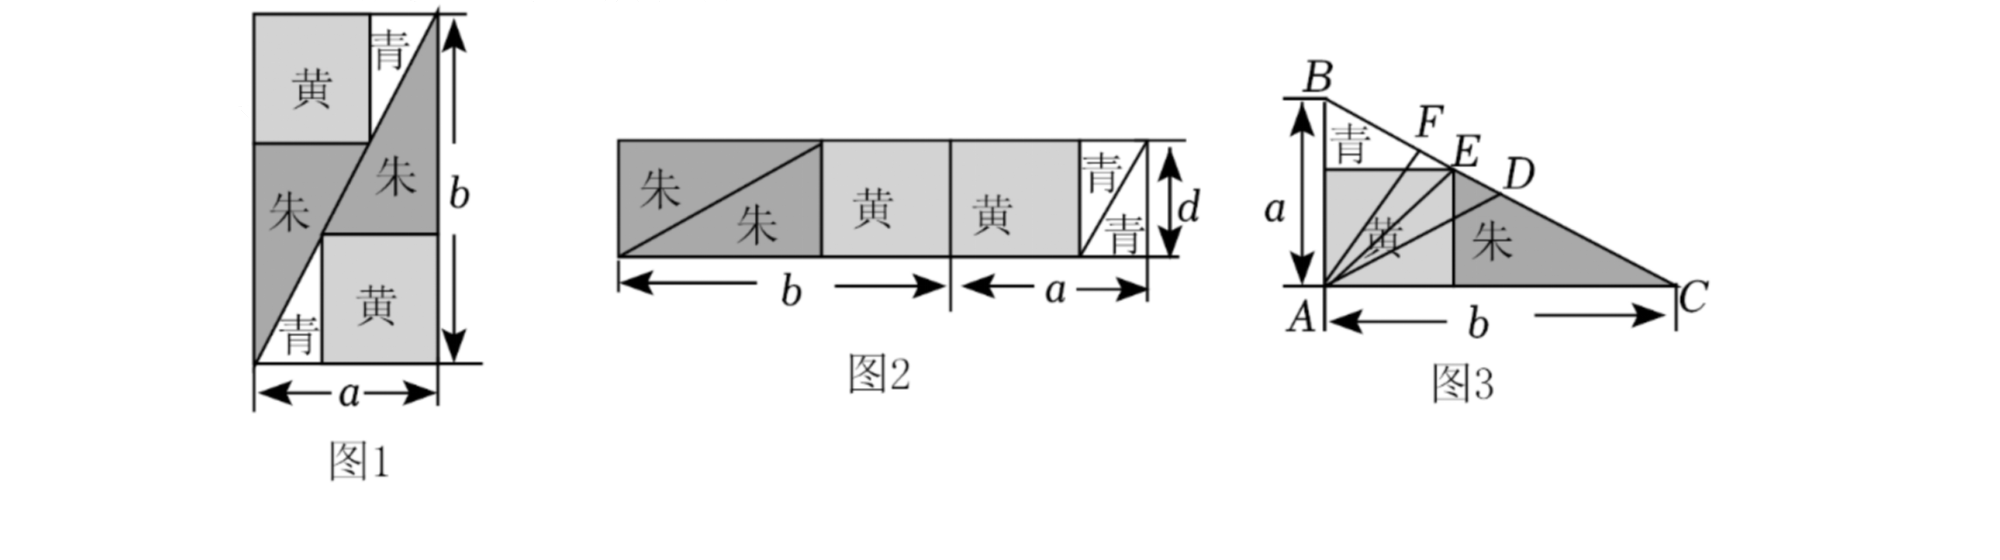
\includegraphics[width=0.86\textwidth]{figures/gao107_q11.png}
\end{center}

①由图 1 和图 2 面积相等得 $d=\dfrac{2ab}{a+b}$　　②由 $AE\geqslant AF$ 可得 $\sqrt{\dfrac{a^2+b^2}2}\geqslant\dfrac{a+b}2$

③由 $AD\geqslant AE$ 可得 $\sqrt{\dfrac{a^2+b^2}2}\geqslant\dfrac{2}{\dfrac1a+\dfrac1b}$　④由 $AD\geqslant AF$ 可得 $a^2+b^2\geqslant2ab$

\ifanswer
\solbegin
\step{对于①，由图 1 和图 2 面积相等得 $ab=(a+b)\times d$，所以 $d=\dfrac{ab}{a+b}$，故①错,}
\step{对于②，因为 $AF\perp BC$，所以 $\dfrac12ab=\dfrac12\sqrt{a^2+b^2}\times AF$,}
\step{所以 $AF=\dfrac{ab}{\sqrt{a^2+b^2}}$，$AE=\sqrt2d=\dfrac{\sqrt2ab}{a+b}$,}
\step{因为 $AE\geqslant AF$，所以 $\dfrac{\sqrt2ab}{a+b}\geqslant\dfrac{ab}{\sqrt{a^2+b^2}}$，整理得 $\sqrt{\dfrac{a^2+b^2}2}\geqslant\dfrac{a+b}2$，故②对,}
\step{对于③，因为 $D$ 是斜边 $BC$ 的中点，所以 $AD=\sqrt{\dfrac{a^2+b^2}2}$,}
\step{因为 $AD\geqslant AE$，所以 $\sqrt{\dfrac{a^2+b^2}2}\geqslant\dfrac{\sqrt2ab}{a+b}$，整理得 $\sqrt{\dfrac{a^2+b^2}2}\geqslant\dfrac{2}{\dfrac1a+\dfrac1b}$，故③对,}
\step{对于④，因为 $AD\geqslant AF$，所以 $\sqrt{\dfrac{a^2+b^2}2}\geqslant\dfrac{ab}{\sqrt{a^2+b^2}}$，整理得 $a^2+b^2\geqslant2ab$,}
\step{故④对,}
\step{故正确的是②③④.}
\solend
\fi

\item 设 $a,b,c,d\in\R$ 且$\lvert a-b\rvert\leqslant2$,$\lvert c-d\rvert\leqslant2$,$\lvert a\rvert\leqslant3$,$\lvert c\rvert\leqslant3$，则 $\lvert ad-bc\rvert$ 的最大值为\blankline[4.4em].% 原卷四处条件间均排半角逗号，照录

\ifanswer
\solbegin
\step{令 $a-b=e$,$c-d=f$，则 $\lvert e\rvert\leqslant2$,$\lvert f\rvert\leqslant2$,$\lvert a\rvert\leqslant3$,$\lvert c\rvert\leqslant3$}
\step{则 $\lvert ad-bc\rvert=\lvert a(c-f)-(a-e)c\rvert=\lvert ce-af\rvert\leqslant\lvert c\rvert\,\lvert e\rvert+\lvert a\rvert\,\lvert f\rvert\leqslant12$,}
\step{则 $\lvert ad-bc\rvert$ 的最大值为 12.}
\solend
\fi

\end{enumerate}

\bigsec{二、选择题}

\begin{enumerate}
\setcounter{enumi}{12}

\item 下列说法正确的是\mbox{（\quad）}

\keepwithprev
A. 若 $a>b>0$，则 $ac^2>bc^2$\qquad\qquad B. 若 $a<b<0$，则 $a^2>ab>b^2$

C. 若 $a>b$，则 $a^2>b^2$\qquad\qquad\qquad D. 若 $a<b$，则 $\dfrac1a>\dfrac1b$

\ifanswer
\solbegin
\step{$A$. 当 $a>b>0$ 时，取 $c=0$，则 $ac^2>bc^2$ 不成立，故 $A$ 错误；}
\step{$B$. 当 $a<b<0$ 时，由不等式的基本性质得 $a^2>ab>b^2>0$，故 $B$ 正确；}
\step{$C$. 当 $a>b$ 时，取 $a=0$，$b=-1$，则 $a^2>b^2$ 不成立，故 $C$ 错误；}
\step{$D$. 当 $a<b$ 时，取 $a=0$，$b=1$，则 $\dfrac1a>\dfrac1b$ 不成立，故 $D$ 错误.}
\step{故选 $B$.}
\solend
\fi

\item 小玲在学习《论语·子路》读到“其身正，不令而行；其身不正，虽令不从”，这句话的
数学含义可以理解为：“身正”是“令行”的\mbox{（\quad）}

\keepwithprev
A. 充分非必要条件\qquad\qquad B. 必要不充分条件

C. 充要条件\qquad\qquad\qquad D. 既非充分又非必要条件

\ifanswer
\solbegin
\step{其身正，不令而行，即身正$\Rightarrow$令行，所以“身正”是“令行”的充分条件；}
\step{又其身不正，虽令不从，即令行$\Rightarrow$身正，所以“身正”是“令行”的必要条件；}
\step{综上，“身正”是“令行”的充要条件. 故选 $C$.}
\solend
\fi

\item 某地对农户抽样调查，结果如下：电冰箱拥有率为 $45\%$，电视机拥有率为 $55\%$，洗衣
机拥有率为 $65\%$，拥有上述三种电器的任意两种的占 $35\%$，三种电器齐全的为 $25\%$，那
么一种电器也没有的农户所占比例是\mbox{（\quad）}

\keepwithprev
A. $12\%$\qquad B. $15\%$\qquad C. $18\%$\qquad D. $20\%$

\ifanswer
\solbegin
\step{设只有电冰箱和电视机的农户有 $a$ 家，只有电冰箱和洗衣机的农户有 $b$ 家,}
\step{只有洗衣机和电视机的农户有 $c$ 家,}
\step{只有电视机、电冰箱、洗衣机的分别有 $d$、$e$、$f$ 家,}
\step{没有任何电器的农户有 $x$ 家,}

\begin{center}
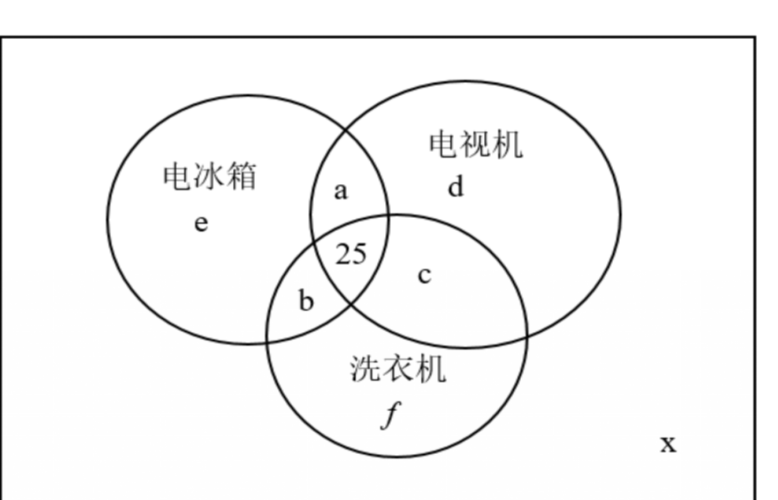
\includegraphics[width=0.42\textwidth]{figures/gao107_q15.png}
\end{center}

\step{所以 $25+a+b+e=45$①，$25+a+c+d=55$②,}
\step{$25+b+c+f=65$③,}
\step{把上面三个式子相加得 $2(a+b+c)+d+e+f=90$④,}
\step{对于拥有上述三种电器的任意两种的占 $35\%$，得 $a+b+c=35$⑤,}
\step{把⑤代入④可得到 $d+e+f=20$⑥,}
\step{因为农户共有 100 家，所以 $25+a+b+c+d+e+f+x=100$,}
\step{把⑤和⑥代入上式得 $x=20$，即一种电器也没有的农户所占比例为 $20\%$.}
\step{故选 $D$.}
\solend
\fi

\item 设 $d>0$，已知 $A,B$ 是两个数集. 若对任意 $x\in A$，都存在 $y\in B$，使得 $\lvert x-y\rvert<d$，则
称 $A$ 是 $B$ 的一个“$d-$邻集”. 现有下列两个命题：① $M=\{a+b\sqrt2\mid a,b\in\Z\}$ 是 $\Q$ 的一个
$\dfrac1{2025}$
一邻集；②若 $A$ 是 $B$ 的一个 $d-$邻集，则 $B$ 也是 $A$ 的一个 $d-$邻集；则\mbox{（\quad）}% 原卷把 d−邻集 的连字符断行后排成“一邻集”，照录

\keepwithprev
A. ①真②假\qquad B. ①假②真\qquad C. ①真②真\qquad D. ①假②假

\ifanswer
\solbegin
\step{对于①，任取 $M$ 中的元素 $x_0=a_0+b_0\sqrt2$,}
\step{则存在 $y_0\in\Q\cap\left(a_0+b_0\sqrt2-\dfrac1{2025},a_0+b_0\sqrt2+\dfrac1{2025}\right)$ 满足题意，故①正确；}
\step{对于②，取 $A=[-1,1]$,$B=[-2,2]$, $A$ 是 $B$ 的 $\dfrac12-$邻集，但反之不成立,}
\step{故②错误；}
\step{故选 $A$.}
\solend
\fi

\end{enumerate}

\bigsec{三、解答题}

\begin{enumerate}
\setcounter{enumi}{16}

\item 设 $a\in\R$，完成下列问题：

（1）求不等式 $3(a+1)x-3>2ax-3a$ 的解集 $M$；

（2）设集合 $A=\{x\mid x^2-ax+a^2-19=0\}$，$B=\{x\mid x^2-5x+6=0\}$，
$C=\{x\mid x^2+2x-8=0\}$. 若 $A\cap B\supset\varnothing$，$A\cap C=\varnothing$，求 $a$ 的值.

\ifanswer
\solbegin
\step{（1）不等式 $3(a+1)x-3>2ax-3a$ 可化为 $(a+3)x>3-3a$,}
\step{当 $a+3>0$，即 $a>-3$ 时，解得 $x>\dfrac{3-3a}{a+3}$,}
\step{当 $a+3=0$，即 $a=-3$ 时，不等式化为 $0\cdot x>12$，无解,}
\step{当 $a+3<0$，即 $a<-3$ 时，解得 $x<\dfrac{3-3a}{a+3}$,}
\step{综上所述，当 $a>-3$ 时，$M=\left(\dfrac{3-3a}{a+3},+\infty\right)$；}
\step{当 $a=-3$ 时，$M=\varnothing$；}
\step{当 $a<-3$ 时，$M=\left(-\infty,\dfrac{3-3a}{a+3}\right)$；}
\step{（2）$B=\{x\mid x^2-5x+6=0\}=\{2,3\}$，$C=\{x\mid x^2+2x-8=0\}=\{2,-4\}$,}
\step{因为 $A\cap B\supset\varnothing$，所以 $A\cap B\neq\varnothing$，又因为 $A\cap C=\varnothing$,}
\step{所以 $3\in A$，$2\notin A$，$-4\notin A$,}
\step{把 $x=3$ 代入方程 $x^2-ax+a^2-19=0$ 得 $9-3a+a^2-19=0$,}
\step{解得 $a=-2$ 或 $a=5$,}
\step{当 $a=-2$ 时，集合 $A=\{x\mid x^2+2x-15=0\}=\{3,-5\}$，符合题意,}
\step{当 $a=5$ 时，集合 $A=\{x\mid x^2-5x+6=0\}=\{3,2\}$，不符合题意，舍去,}
\step{综上所述，$a$ 的值为 $-2$.}
\solend
\fi

\item 完成下列问题：

（1）设 $x$、$y\in\R$，且 $x+y>5$，用反证法证明：$x>3$ 或 $y>2$；

（2）设 $x>0$，$a=x+1$，$b=\sqrt{x^2+7x+1}$，求 $\dfrac ba$ 的最大值.

\ifanswer
\solbegin
\step{（1）假设 $x\leqslant3$ 且 $y\leqslant2$，则 $x+y\leqslant3+2=5$，这与已知 $x+y>5$ 矛盾,}
\step{故 $x>3$ 或 $y>2$；}
\step{（2）$x>0$，$a=x+1$，$b=\sqrt{x^2+7x+1}$,}
\step{则 $\dfrac ba=\dfrac{\sqrt{x^2+7x+1}}{x+1}=\sqrt{\dfrac{x^2+7x+1}{x^2+2x+1}}=\sqrt{\dfrac{x^2+2x+1+5x}{x^2+2x+1}}$}
\step{$=\sqrt{1+\dfrac{5x}{x^2+2x+1}}=\sqrt{1+\dfrac{5}{x+\dfrac1x+2}}\leqslant\sqrt{1+\dfrac{5}{2\sqrt{x\cdot\dfrac1x}+2}}=\dfrac32$,}
\step{当且仅当 $x=\dfrac1x$，即 $x=1$ 时取等号，故 $\dfrac ba$ 的最大值为 $\dfrac32$.}
\solend
\fi

\item 已知函数 $f(x)=\lvert2x-a\rvert+a$.

（1）当 $a=2$ 时，求不等式 $f(x)\leqslant6+\lvert x+2\rvert$ 的解集；

（2）设 $g(x)=\lvert2x-1\rvert$，若不等式 $f(x)+g(x)\geqslant3$ 对一切 $x\in\R$ 恒成立，求实数 $a$ 的取值
范围.

\ifanswer
\solbegin
\ansspace*
\step{（1）$a=2$ 时，$f(x)=\lvert2x-2\rvert+2$,}
\step{则 $f(x)\leqslant6+\lvert x+2\rvert\Leftrightarrow\lvert2x-2\rvert+2\leqslant6+\lvert x+2\rvert$，即 $\lvert2x-2\rvert-\lvert x+2\rvert\leqslant4$,}
\step{当 $x<-2$ 时，$2-2x+x+2\leqslant4$，解得 $x\geqslant0$，与 $x<-2$ 取交集得 $\varnothing$,}
\step{当 $-2\leqslant x\leqslant1$ 时，$2-2x-x-2\leqslant4$，解得 $x\geqslant-\dfrac43$,}
\step{与 $-2\leqslant x\leqslant1$ 取交集得 $-\dfrac43\leqslant x\leqslant1$,}
\step{当 $x>1$ 时，$2x-2-x-2\leqslant4$，解得 $x\leqslant8$，与 $x>1$ 取交集得 $1<x\leqslant8$,}
\step{综上，不等式 $f(x)\leqslant6+\lvert x+2\rvert$ 的解集为 $\left\{x\,\middle|\,-\dfrac43\leqslant x\leqslant8\right\}$；}
\step{（2）$f(x)+g(x)\geqslant3$，即 $\lvert2x-a\rvert+a+\lvert2x-1\rvert\geqslant3$,}
\step{故 $\lvert2x-a\rvert+\lvert2x-1\rvert\geqslant3-a$,}
\step{当 $a\geqslant3$ 时，不等式显然成立,}
\step{当 $a<3$ 时,}
\step{由三角不等式得 $\lvert2x-a\rvert+\lvert2x-1\rvert\geqslant\lvert2x-a-(2x-1)\rvert=\lvert1-a\rvert$,}
\step{当且仅当 $(2x-a)(2x-1)\leqslant0$ 时取等号，因此 $\lvert1-a\rvert\geqslant3-a$,}
\step{平方得 $(1-a)^2\geqslant(3-a)^2$，解得 $a\geqslant2$，故 $2\leqslant a<3$.}
\step{综上，实数 $a$ 的取值范围是 $a\geqslant2$.}
\solend
\fi

\item 对于集合 $A,B$，定义集合 $A-B=\{x\mid x\in A$ 且 $x\notin B\}$.

（1）若 $A=\{1,2,3,4\}$,$B=\{3,4,5\}$，求集合 $A-B$ 和 $B-A$；

（2）给定集合 $A,B$，求所有满足方程组
\[
\begin{cases}
X\cap(A\cup B)=X\\
A\cap(B\cup X)=A\\
B\cap(A\cup X)=B\\
X\cap(A\cap B)=\varnothing
\end{cases}
\]
的集合 $X$（用 $A,B$ 表示）；

（3）用 $\lvert M\rvert$ 表示集合 $M$ 中的元素个数. 给定正整数 $n$，集合 $S=\{1,2,\cdots,n\}$. 对于实数
集的非空有限子集 $A,B$，定义集合 $C=\{x\mid x=a+b,a\in A,b\in B\}$. 求证：

$\lvert A-S\rvert+\lvert B-S\rvert+\lvert S-C\rvert\geqslant1$.

\ifanswer
\solbegin
\step{（1）由 $A=\{1,2,3,4\}$,$B=\{3,4,5\}$，则 $A-B=\{1,2\}$,$B-A=\{5\}$；}
\step{（2）由
$\begin{cases}
X\cap(A\cup B)=X\\
X\cap(A\cap B)=\varnothing
\end{cases}$，
得 $X\subseteq A-B$ 或 $X\subseteq B-A$,}
\step{再结合
$\begin{cases}
A\cap(B\cup X)=A\\
B\cap(A\cup X)=B
\end{cases}$，
得 $X=(A-B)\cup(B-A)$,}
\step{所以 $X=(A-B)\cup(B-A)$；}
\step{（3）$\lvert X\rvert$ 表示集合 $X$ 中的元素个数，则 $\lvert X\rvert\geqslant0$,}
\step{若 $A\cup B$ 中至少含有一个不在 $S$ 中的元素，则 $\lvert A-S\rvert+\lvert B-S\rvert\geqslant1$,}
\step{即 $\lvert A-S\rvert+\lvert B-S\rvert+\lvert S-C\rvert\geqslant1$.}
\step{若 $A\subseteq S$，且 $B\subseteq S$，则 $\lvert A-S\rvert=\lvert B-S\rvert=0$.}
\step{此时 $A$ 中最小的元素 $a\geqslant1$,$B$ 中最小的元素 $b\geqslant1$.}
\step{所以 $C$ 中最小的元素 $a+b\geqslant2$，则 $1\notin C$,}
\step{因为 $S=\{1,2,\cdots,n\}$，所以 $\lvert S-C\rvert\geqslant1$，即 $\lvert A-S\rvert+\lvert B-S\rvert+\lvert S-C\rvert\geqslant1$.}
\step{综上所述，$\lvert A-S\rvert+\lvert B-S\rvert+\lvert S-C\rvert\geqslant1$.}
\solend
\fi

\end{enumerate}

\end{document}
"
% 紧凑版：xelatex "\def\iscompact{1}% 高一107_曹杨二中_10月月考.tex
%   —— 高一上数学“2026-2027 年曹杨二中高一上 10 月月考”（试卷版/答案版）
% 试卷版：xelatex 高一107_曹杨二中_10月月考.tex
% 答案版：xelatex "\def\isanswer{1}\input{高一107_曹杨二中_10月月考.tex}"
% 紧凑版：xelatex "\def\iscompact{1}\input{高一107_曹杨二中_10月月考.tex}"
%
% 原始材料：微信公众号“魔都数学加油站”文章，作者破晓，2026-11-03 17:19 发布；
% 连载“27学年高一107”，原文标题“27学年高一107——2026-2027年上海市曹杨二中高一上10月月考”；
% 原文链接：https://mp.weixin.qq.com/s/IF4uB7aDNv-snYwbGMoDiQ。
% 正文为 10 张 PNG 页（第 1、2、4、6—9 页 4762×6735，第 3、5、10 页 2560×3620），题目下印有【解析】，为讲评版。
% 题目、解析均据原图转录；卷面水印及公众号页脚未录入。
% 第 11 题题干的三幅“出入相补”图（图 1—图 3）与第 15 题解析的三圆文氏图裁自原图、
% 去粉色水印转灰度（gao107_q11.png、gao107_q15.png），第 11 题图属题干（三版都出）、
% 第 15 题图属解析（仅答案版显示）。
%
% 卷首标题：原卷印作“2026-2027 年曹杨二中高一上 10 月月考”（公众号标题中的“上海市”
% 卷面标题行没有，本稿照卷面），年份区间按全稿惯例排 en dash；原卷未印副标题，本稿按题目内容
% 标为“集合与常用逻辑用语、不等式”。
%
% 与原卷的排版差异：
%   ① 原文从第 3 题起，填空题编号为 3—12、选择题为 13—16、解答题为 17—20，本稿保留原题号；
%   ② 原卷每题下直接印【解析】，本稿按全稿惯例将解析置于答案版；第 4 题只印【答案】另提 \ans{}；
%   ③ 原卷未印副标题，本稿按“知识模块”口径补出；
%   ④ 原卷填空横线按全稿惯例排为 \blankline[4.4em]；解答题按惯例加 \ansspace；选择题括号排
%      \mbox{（\quad）}、选项段前按惯例加 \keepwithprev；
%   ⑤ 原卷数集字母粗体与斜体混用（第 3 题 $\mathbf{R}$、第 4 题斜体 $R$、第 16 题粗体
%      $\mathbf{Z}$、$\mathbf{Q}$ 等），按全稿惯例统一改 \R、\Z、\Q。
%
% 原卷存疑：第 10 题解析“由 $\Delta=16m^2-8(2m^2+3m-2)\geqslant0$ 得 $m\leqslant\dfrac23$”
% 行末原卷无句读，照录。第 16 题解析②“取 $A=[-1,1]$，$B=[-2,2]$，$A$ 是 $B$ 的
% $\dfrac12$-邻集，但反之不成立”，据以判①真②假，照录。
%
% 行数核对：逐题数 \step/\stepm 条数，合计 112 条（Q3：5；Q4：0；Q5：2；Q6：2；Q7：2；
% Q8：4；Q9：8；Q10：4；Q11：9；Q12：3；Q13：5；Q14：3；Q15：12；Q16：5；Q17：15；
% Q18：6；Q19：15；Q20：12），与原卷印刷行逐题相等。第 4 题只印【答案】，提 \ans{}，
% 不计入 \step 账。
%
\documentclass[a4paper,11pt]{article}
\usepackage{common}

\begin{document}

\examtitlest[3]{2026--2027 年曹杨二中高一上 10 月月考}{集合与常用逻辑用语、不等式}

\bigsec{一、填空题}

\begin{enumerate}
\setcounter{enumi}{2}

\item 设 $a\in\R$，若 $3\in\{\sqrt3,a^2,a\}$，则 $a=$\blankline[4.4em].

\ifanswer
\solbegin
\step{因为 $3\in\{\sqrt3,a^2,a\}$，所以 $a^2=3$，解得 $a=\sqrt3$ 或 $a=-\sqrt3$,}
\step{当 $a=\sqrt3$ 时，集合为 $\{\sqrt3,3,\sqrt3\}$，不满足集合元素的互异性，舍去；}
\step{当 $a=-\sqrt3$ 时，集合为 $\{\sqrt3,3,-\sqrt3\}$，符合要求；}
\step{若 $a=3$，此时集合为 $\{\sqrt3,9,3\}$，符合要求；}
\step{综上，$a$ 为 $-\sqrt3$ 或 $3$.}
\solend
\fi

\item 设 $a\in\R$，已知集合 $A=\{x\mid x\leqslant a\}$，$B=\{x\mid x>2\}$. 若 $A\cup B=\R$，则 $a$ 的取值范围是\blankline[4.4em].

\ifanswer
\ans{$a\geqslant2$}
\fi

\item 设 $x>0$，$y>0$ 且 $x+3y=1$，则 $xy$ 的最大值为\blankline[4.4em].

\ifanswer
\solbegin
\step{由于 $x>0$，$y>0$ 且 $x+3y=1$，则 $1=x+3y\geqslant2\sqrt{3xy}$，得 $xy\leqslant\dfrac1{12}$,}
\step{当且仅当 $x=3y=\dfrac12$ 时取等号，则 $xy$ 的最大值为 $\dfrac1{12}$.}
\solend
\fi

\item 设 $a\in\R$，若集合$\left\{x\,\middle|\,\dfrac{ax}{x-1}=x\right\}$有且仅有两个子集，则 $a=$\blankline[4.4em].

\ifanswer
\solbegin
\step{由 $\dfrac{ax}{x-1}=x$ 得 $ax=x(x-1)$，即 $x(x-a-1)=0$,}
\step{所以此方程有两个相等的（不等于 1）的实数根或有一根为 1，所以 $a=-1$ 或 $0$.}
\solend
\fi

\item 已知全集 $U=\{x\mid x^2-8x-20<0\}$，集合 $A=\{x\mid 1-x^2>0$ 且 $x<0\}$，则 $\overline A=$\blankline[4.4em].

\ifanswer
\solbegin
\step{$U=\{x\mid-2<x<10\}$，$A=\{x\mid-1<x<0\}$,}
\step{所以 $\overline A=\{x\mid-2<x\leqslant-1$ 或 $0\leqslant x<10\}$.}
\solend
\fi

\item 设 $a,b\in\R$，若不等式 $-x^2-ax+b\geqslant0$ 的解集为 $[-2,3]$，则不等式 $\lvert ax+b\rvert<5$ 的解集为\blankline[4.4em].

\ifanswer
\solbegin
\step{由不等式 $-x^2-ax+b\geqslant0$ 的解集为 $[-2,3]$,}
\step{得 $-2$、$3$ 是方程 $-x^2-ax+b=0$ 的两个根，所以 $a=-1$，$b=6$.}
\step{解不等式 $\lvert-x+6\rvert<5$，得 $-5<x-6<5$，解得 $1<x<11$,}
\step{即所求不等式的解集为 $(1,11)$.}
\solend
\fi

\item 某货运卡车以 $x$ 千米／时的速度匀速行驶 300 千米，按交通法规限制 $50\leqslant x\leqslant100$，假设
柴油的价格为每升 6 元，汽车每小时耗油 $\left(4+\dfrac{x^2}{420}\right)$ 升，司机工资为每小时 46 元. 则当
$x=$\blankline[4.4em]（千米／时），这次行车的总费用（油费与司机工资的总和）最低.

\ifanswer
\solbegin
\step{因为卡车行驶 300 千米，速度为 $x$ 千米／时,}
\step{因此总用时为 $t=\dfrac{300}{x}$ 小时，其中 $50\leqslant x\leqslant100$,}
\step{每小时油费为 $6\cdot\left(4+\dfrac{x^2}{420}\right)$ 元，每小时司机工资为 46 元，因}
\step{此每小时总支出为 $6\cdot\left(4+\dfrac{x^2}{420}\right)+46=70+\dfrac{x^2}{70}$ 元.}
\step{设全程总费用为 $y$，则 $y=\dfrac{300}{x}\cdot\left(70+\dfrac{x^2}{70}\right)=\dfrac{21000}{x}+\dfrac{30x}{7}$,}
\step{因为 $50\leqslant x\leqslant100$，$\dfrac{21000}{x}+\dfrac{30x}{7}\geqslant2\sqrt{\dfrac{21000}{x}\cdot\dfrac{30x}{7}}=600$,}
\step{当且仅当 $\dfrac{21000}{x}=\dfrac{30x}{7}$，即 $x=70$ 时取等号，且 $70\in[50,100]$,}
\step{因此当 $x=70$ 千米／时，行车的总费用（油费与司机工资的总和）最低.}
\solend
\fi

\item 设 $x_1$、$x_2$ 是关于 $x$ 的方程 $2x^2-4mx+2m^2+3m-2=0$ 的两个实数根，则 $x_1^2+x_2^2$ 的最小值为\blankline[4.4em].

\ifanswer
\solbegin
\step{由题意得 $x_1+x_2=2m$，$x_1x_2=m^2+\dfrac{3m}{2}-1$,}
\step{由 $\Delta=16m^2-8(2m^2+3m-2)\geqslant0$ 得 $m\leqslant\dfrac23$}
\step{所以 $x_1^2+x_1^2=(x_1+x_2)^2-2x_1x_2=4m^2-2m^2+3m+2=2m^2-3m+2$,% 原卷左端作 x_1²+x_1²，照录
}
\step{结合二次函数的性质得，当 $m=\dfrac23$ 时取得最小值 $\dfrac89$.}
\solend
\fi

\item 小玲在钻研《九章算术》中“勾股容方”问题“今有勾五步，股十二步，问勾中容方几
何？”时，发现魏晋时期数学家刘徽在其《九章算术注》中利用出入相补原理给出了这个
问题的一般解法：如图 1，用对角线将长和宽分别为 $b$ 和 $a$ 的矩形分成两个直角三角形，
每个直角三角形再分成一个内接正方形（黄）和两个小直角三角形（朱、青）. 将三种颜色
的图形进行重组，得到如图 2 所示的矩形，该矩形长为 $a+b$，宽为内接正方形的边长
$d$. 由刘徽构造的图形可以得到许多重要的结论，如图 3，设 $D$ 为斜边 $BC$ 的中点，作直
角三角形 $ABC$ 的内接正方形对角线 $AE$，过点 $A$ 作 $AF\perp BC$ 于点 $F$，则下列四个推理中
正确的序号是\blankline[4.4em].

\begin{center}
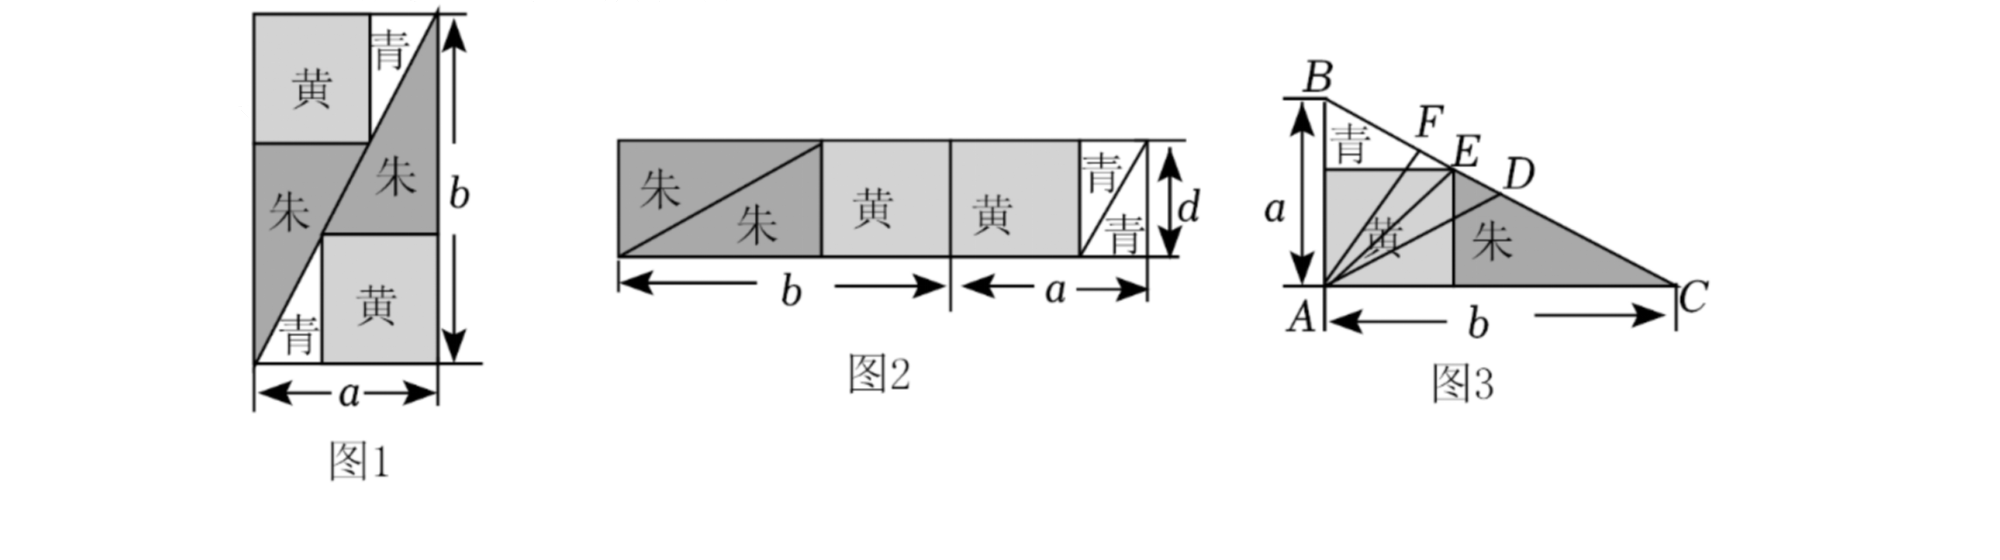
\includegraphics[width=0.86\textwidth]{figures/gao107_q11.png}
\end{center}

①由图 1 和图 2 面积相等得 $d=\dfrac{2ab}{a+b}$　　②由 $AE\geqslant AF$ 可得 $\sqrt{\dfrac{a^2+b^2}2}\geqslant\dfrac{a+b}2$

③由 $AD\geqslant AE$ 可得 $\sqrt{\dfrac{a^2+b^2}2}\geqslant\dfrac{2}{\dfrac1a+\dfrac1b}$　④由 $AD\geqslant AF$ 可得 $a^2+b^2\geqslant2ab$

\ifanswer
\solbegin
\step{对于①，由图 1 和图 2 面积相等得 $ab=(a+b)\times d$，所以 $d=\dfrac{ab}{a+b}$，故①错,}
\step{对于②，因为 $AF\perp BC$，所以 $\dfrac12ab=\dfrac12\sqrt{a^2+b^2}\times AF$,}
\step{所以 $AF=\dfrac{ab}{\sqrt{a^2+b^2}}$，$AE=\sqrt2d=\dfrac{\sqrt2ab}{a+b}$,}
\step{因为 $AE\geqslant AF$，所以 $\dfrac{\sqrt2ab}{a+b}\geqslant\dfrac{ab}{\sqrt{a^2+b^2}}$，整理得 $\sqrt{\dfrac{a^2+b^2}2}\geqslant\dfrac{a+b}2$，故②对,}
\step{对于③，因为 $D$ 是斜边 $BC$ 的中点，所以 $AD=\sqrt{\dfrac{a^2+b^2}2}$,}
\step{因为 $AD\geqslant AE$，所以 $\sqrt{\dfrac{a^2+b^2}2}\geqslant\dfrac{\sqrt2ab}{a+b}$，整理得 $\sqrt{\dfrac{a^2+b^2}2}\geqslant\dfrac{2}{\dfrac1a+\dfrac1b}$，故③对,}
\step{对于④，因为 $AD\geqslant AF$，所以 $\sqrt{\dfrac{a^2+b^2}2}\geqslant\dfrac{ab}{\sqrt{a^2+b^2}}$，整理得 $a^2+b^2\geqslant2ab$,}
\step{故④对,}
\step{故正确的是②③④.}
\solend
\fi

\item 设 $a,b,c,d\in\R$ 且$\lvert a-b\rvert\leqslant2$,$\lvert c-d\rvert\leqslant2$,$\lvert a\rvert\leqslant3$,$\lvert c\rvert\leqslant3$，则 $\lvert ad-bc\rvert$ 的最大值为\blankline[4.4em].% 原卷四处条件间均排半角逗号，照录

\ifanswer
\solbegin
\step{令 $a-b=e$,$c-d=f$，则 $\lvert e\rvert\leqslant2$,$\lvert f\rvert\leqslant2$,$\lvert a\rvert\leqslant3$,$\lvert c\rvert\leqslant3$}
\step{则 $\lvert ad-bc\rvert=\lvert a(c-f)-(a-e)c\rvert=\lvert ce-af\rvert\leqslant\lvert c\rvert\,\lvert e\rvert+\lvert a\rvert\,\lvert f\rvert\leqslant12$,}
\step{则 $\lvert ad-bc\rvert$ 的最大值为 12.}
\solend
\fi

\end{enumerate}

\bigsec{二、选择题}

\begin{enumerate}
\setcounter{enumi}{12}

\item 下列说法正确的是\mbox{（\quad）}

\keepwithprev
A. 若 $a>b>0$，则 $ac^2>bc^2$\qquad\qquad B. 若 $a<b<0$，则 $a^2>ab>b^2$

C. 若 $a>b$，则 $a^2>b^2$\qquad\qquad\qquad D. 若 $a<b$，则 $\dfrac1a>\dfrac1b$

\ifanswer
\solbegin
\step{$A$. 当 $a>b>0$ 时，取 $c=0$，则 $ac^2>bc^2$ 不成立，故 $A$ 错误；}
\step{$B$. 当 $a<b<0$ 时，由不等式的基本性质得 $a^2>ab>b^2>0$，故 $B$ 正确；}
\step{$C$. 当 $a>b$ 时，取 $a=0$，$b=-1$，则 $a^2>b^2$ 不成立，故 $C$ 错误；}
\step{$D$. 当 $a<b$ 时，取 $a=0$，$b=1$，则 $\dfrac1a>\dfrac1b$ 不成立，故 $D$ 错误.}
\step{故选 $B$.}
\solend
\fi

\item 小玲在学习《论语·子路》读到“其身正，不令而行；其身不正，虽令不从”，这句话的
数学含义可以理解为：“身正”是“令行”的\mbox{（\quad）}

\keepwithprev
A. 充分非必要条件\qquad\qquad B. 必要不充分条件

C. 充要条件\qquad\qquad\qquad D. 既非充分又非必要条件

\ifanswer
\solbegin
\step{其身正，不令而行，即身正$\Rightarrow$令行，所以“身正”是“令行”的充分条件；}
\step{又其身不正，虽令不从，即令行$\Rightarrow$身正，所以“身正”是“令行”的必要条件；}
\step{综上，“身正”是“令行”的充要条件. 故选 $C$.}
\solend
\fi

\item 某地对农户抽样调查，结果如下：电冰箱拥有率为 $45\%$，电视机拥有率为 $55\%$，洗衣
机拥有率为 $65\%$，拥有上述三种电器的任意两种的占 $35\%$，三种电器齐全的为 $25\%$，那
么一种电器也没有的农户所占比例是\mbox{（\quad）}

\keepwithprev
A. $12\%$\qquad B. $15\%$\qquad C. $18\%$\qquad D. $20\%$

\ifanswer
\solbegin
\step{设只有电冰箱和电视机的农户有 $a$ 家，只有电冰箱和洗衣机的农户有 $b$ 家,}
\step{只有洗衣机和电视机的农户有 $c$ 家,}
\step{只有电视机、电冰箱、洗衣机的分别有 $d$、$e$、$f$ 家,}
\step{没有任何电器的农户有 $x$ 家,}

\begin{center}
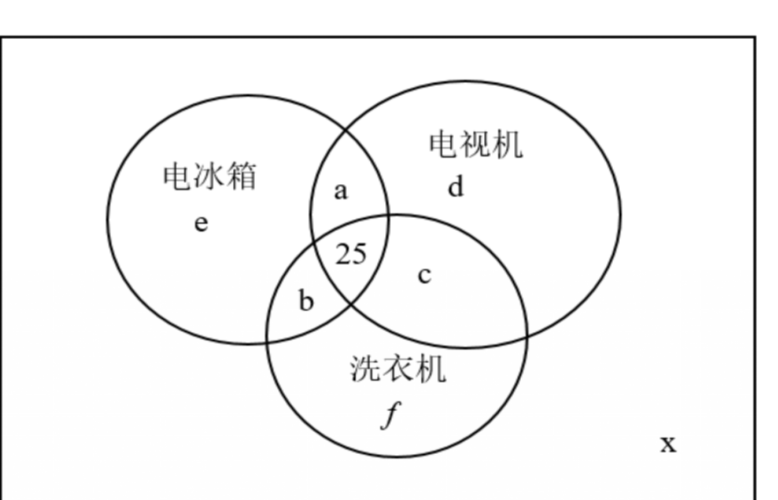
\includegraphics[width=0.42\textwidth]{figures/gao107_q15.png}
\end{center}

\step{所以 $25+a+b+e=45$①，$25+a+c+d=55$②,}
\step{$25+b+c+f=65$③,}
\step{把上面三个式子相加得 $2(a+b+c)+d+e+f=90$④,}
\step{对于拥有上述三种电器的任意两种的占 $35\%$，得 $a+b+c=35$⑤,}
\step{把⑤代入④可得到 $d+e+f=20$⑥,}
\step{因为农户共有 100 家，所以 $25+a+b+c+d+e+f+x=100$,}
\step{把⑤和⑥代入上式得 $x=20$，即一种电器也没有的农户所占比例为 $20\%$.}
\step{故选 $D$.}
\solend
\fi

\item 设 $d>0$，已知 $A,B$ 是两个数集. 若对任意 $x\in A$，都存在 $y\in B$，使得 $\lvert x-y\rvert<d$，则
称 $A$ 是 $B$ 的一个“$d-$邻集”. 现有下列两个命题：① $M=\{a+b\sqrt2\mid a,b\in\Z\}$ 是 $\Q$ 的一个
$\dfrac1{2025}$
一邻集；②若 $A$ 是 $B$ 的一个 $d-$邻集，则 $B$ 也是 $A$ 的一个 $d-$邻集；则\mbox{（\quad）}% 原卷把 d−邻集 的连字符断行后排成“一邻集”，照录

\keepwithprev
A. ①真②假\qquad B. ①假②真\qquad C. ①真②真\qquad D. ①假②假

\ifanswer
\solbegin
\step{对于①，任取 $M$ 中的元素 $x_0=a_0+b_0\sqrt2$,}
\step{则存在 $y_0\in\Q\cap\left(a_0+b_0\sqrt2-\dfrac1{2025},a_0+b_0\sqrt2+\dfrac1{2025}\right)$ 满足题意，故①正确；}
\step{对于②，取 $A=[-1,1]$,$B=[-2,2]$, $A$ 是 $B$ 的 $\dfrac12-$邻集，但反之不成立,}
\step{故②错误；}
\step{故选 $A$.}
\solend
\fi

\end{enumerate}

\bigsec{三、解答题}

\begin{enumerate}
\setcounter{enumi}{16}

\item 设 $a\in\R$，完成下列问题：

（1）求不等式 $3(a+1)x-3>2ax-3a$ 的解集 $M$；

（2）设集合 $A=\{x\mid x^2-ax+a^2-19=0\}$，$B=\{x\mid x^2-5x+6=0\}$，
$C=\{x\mid x^2+2x-8=0\}$. 若 $A\cap B\supset\varnothing$，$A\cap C=\varnothing$，求 $a$ 的值.

\ifanswer
\solbegin
\step{（1）不等式 $3(a+1)x-3>2ax-3a$ 可化为 $(a+3)x>3-3a$,}
\step{当 $a+3>0$，即 $a>-3$ 时，解得 $x>\dfrac{3-3a}{a+3}$,}
\step{当 $a+3=0$，即 $a=-3$ 时，不等式化为 $0\cdot x>12$，无解,}
\step{当 $a+3<0$，即 $a<-3$ 时，解得 $x<\dfrac{3-3a}{a+3}$,}
\step{综上所述，当 $a>-3$ 时，$M=\left(\dfrac{3-3a}{a+3},+\infty\right)$；}
\step{当 $a=-3$ 时，$M=\varnothing$；}
\step{当 $a<-3$ 时，$M=\left(-\infty,\dfrac{3-3a}{a+3}\right)$；}
\step{（2）$B=\{x\mid x^2-5x+6=0\}=\{2,3\}$，$C=\{x\mid x^2+2x-8=0\}=\{2,-4\}$,}
\step{因为 $A\cap B\supset\varnothing$，所以 $A\cap B\neq\varnothing$，又因为 $A\cap C=\varnothing$,}
\step{所以 $3\in A$，$2\notin A$，$-4\notin A$,}
\step{把 $x=3$ 代入方程 $x^2-ax+a^2-19=0$ 得 $9-3a+a^2-19=0$,}
\step{解得 $a=-2$ 或 $a=5$,}
\step{当 $a=-2$ 时，集合 $A=\{x\mid x^2+2x-15=0\}=\{3,-5\}$，符合题意,}
\step{当 $a=5$ 时，集合 $A=\{x\mid x^2-5x+6=0\}=\{3,2\}$，不符合题意，舍去,}
\step{综上所述，$a$ 的值为 $-2$.}
\solend
\fi

\item 完成下列问题：

（1）设 $x$、$y\in\R$，且 $x+y>5$，用反证法证明：$x>3$ 或 $y>2$；

（2）设 $x>0$，$a=x+1$，$b=\sqrt{x^2+7x+1}$，求 $\dfrac ba$ 的最大值.

\ifanswer
\solbegin
\step{（1）假设 $x\leqslant3$ 且 $y\leqslant2$，则 $x+y\leqslant3+2=5$，这与已知 $x+y>5$ 矛盾,}
\step{故 $x>3$ 或 $y>2$；}
\step{（2）$x>0$，$a=x+1$，$b=\sqrt{x^2+7x+1}$,}
\step{则 $\dfrac ba=\dfrac{\sqrt{x^2+7x+1}}{x+1}=\sqrt{\dfrac{x^2+7x+1}{x^2+2x+1}}=\sqrt{\dfrac{x^2+2x+1+5x}{x^2+2x+1}}$}
\step{$=\sqrt{1+\dfrac{5x}{x^2+2x+1}}=\sqrt{1+\dfrac{5}{x+\dfrac1x+2}}\leqslant\sqrt{1+\dfrac{5}{2\sqrt{x\cdot\dfrac1x}+2}}=\dfrac32$,}
\step{当且仅当 $x=\dfrac1x$，即 $x=1$ 时取等号，故 $\dfrac ba$ 的最大值为 $\dfrac32$.}
\solend
\fi

\item 已知函数 $f(x)=\lvert2x-a\rvert+a$.

（1）当 $a=2$ 时，求不等式 $f(x)\leqslant6+\lvert x+2\rvert$ 的解集；

（2）设 $g(x)=\lvert2x-1\rvert$，若不等式 $f(x)+g(x)\geqslant3$ 对一切 $x\in\R$ 恒成立，求实数 $a$ 的取值
范围.

\ifanswer
\solbegin
\ansspace*
\step{（1）$a=2$ 时，$f(x)=\lvert2x-2\rvert+2$,}
\step{则 $f(x)\leqslant6+\lvert x+2\rvert\Leftrightarrow\lvert2x-2\rvert+2\leqslant6+\lvert x+2\rvert$，即 $\lvert2x-2\rvert-\lvert x+2\rvert\leqslant4$,}
\step{当 $x<-2$ 时，$2-2x+x+2\leqslant4$，解得 $x\geqslant0$，与 $x<-2$ 取交集得 $\varnothing$,}
\step{当 $-2\leqslant x\leqslant1$ 时，$2-2x-x-2\leqslant4$，解得 $x\geqslant-\dfrac43$,}
\step{与 $-2\leqslant x\leqslant1$ 取交集得 $-\dfrac43\leqslant x\leqslant1$,}
\step{当 $x>1$ 时，$2x-2-x-2\leqslant4$，解得 $x\leqslant8$，与 $x>1$ 取交集得 $1<x\leqslant8$,}
\step{综上，不等式 $f(x)\leqslant6+\lvert x+2\rvert$ 的解集为 $\left\{x\,\middle|\,-\dfrac43\leqslant x\leqslant8\right\}$；}
\step{（2）$f(x)+g(x)\geqslant3$，即 $\lvert2x-a\rvert+a+\lvert2x-1\rvert\geqslant3$,}
\step{故 $\lvert2x-a\rvert+\lvert2x-1\rvert\geqslant3-a$,}
\step{当 $a\geqslant3$ 时，不等式显然成立,}
\step{当 $a<3$ 时,}
\step{由三角不等式得 $\lvert2x-a\rvert+\lvert2x-1\rvert\geqslant\lvert2x-a-(2x-1)\rvert=\lvert1-a\rvert$,}
\step{当且仅当 $(2x-a)(2x-1)\leqslant0$ 时取等号，因此 $\lvert1-a\rvert\geqslant3-a$,}
\step{平方得 $(1-a)^2\geqslant(3-a)^2$，解得 $a\geqslant2$，故 $2\leqslant a<3$.}
\step{综上，实数 $a$ 的取值范围是 $a\geqslant2$.}
\solend
\fi

\item 对于集合 $A,B$，定义集合 $A-B=\{x\mid x\in A$ 且 $x\notin B\}$.

（1）若 $A=\{1,2,3,4\}$,$B=\{3,4,5\}$，求集合 $A-B$ 和 $B-A$；

（2）给定集合 $A,B$，求所有满足方程组
\[
\begin{cases}
X\cap(A\cup B)=X\\
A\cap(B\cup X)=A\\
B\cap(A\cup X)=B\\
X\cap(A\cap B)=\varnothing
\end{cases}
\]
的集合 $X$（用 $A,B$ 表示）；

（3）用 $\lvert M\rvert$ 表示集合 $M$ 中的元素个数. 给定正整数 $n$，集合 $S=\{1,2,\cdots,n\}$. 对于实数
集的非空有限子集 $A,B$，定义集合 $C=\{x\mid x=a+b,a\in A,b\in B\}$. 求证：

$\lvert A-S\rvert+\lvert B-S\rvert+\lvert S-C\rvert\geqslant1$.

\ifanswer
\solbegin
\step{（1）由 $A=\{1,2,3,4\}$,$B=\{3,4,5\}$，则 $A-B=\{1,2\}$,$B-A=\{5\}$；}
\step{（2）由
$\begin{cases}
X\cap(A\cup B)=X\\
X\cap(A\cap B)=\varnothing
\end{cases}$，
得 $X\subseteq A-B$ 或 $X\subseteq B-A$,}
\step{再结合
$\begin{cases}
A\cap(B\cup X)=A\\
B\cap(A\cup X)=B
\end{cases}$，
得 $X=(A-B)\cup(B-A)$,}
\step{所以 $X=(A-B)\cup(B-A)$；}
\step{（3）$\lvert X\rvert$ 表示集合 $X$ 中的元素个数，则 $\lvert X\rvert\geqslant0$,}
\step{若 $A\cup B$ 中至少含有一个不在 $S$ 中的元素，则 $\lvert A-S\rvert+\lvert B-S\rvert\geqslant1$,}
\step{即 $\lvert A-S\rvert+\lvert B-S\rvert+\lvert S-C\rvert\geqslant1$.}
\step{若 $A\subseteq S$，且 $B\subseteq S$，则 $\lvert A-S\rvert=\lvert B-S\rvert=0$.}
\step{此时 $A$ 中最小的元素 $a\geqslant1$,$B$ 中最小的元素 $b\geqslant1$.}
\step{所以 $C$ 中最小的元素 $a+b\geqslant2$，则 $1\notin C$,}
\step{因为 $S=\{1,2,\cdots,n\}$，所以 $\lvert S-C\rvert\geqslant1$，即 $\lvert A-S\rvert+\lvert B-S\rvert+\lvert S-C\rvert\geqslant1$.}
\step{综上所述，$\lvert A-S\rvert+\lvert B-S\rvert+\lvert S-C\rvert\geqslant1$.}
\solend
\fi

\end{enumerate}

\end{document}
"
%
% 原始材料：微信公众号“魔都数学加油站”文章，作者破晓，2026-11-03 17:19 发布；
% 连载“27学年高一107”，原文标题“27学年高一107——2026-2027年上海市曹杨二中高一上10月月考”；
% 原文链接：https://mp.weixin.qq.com/s/IF4uB7aDNv-snYwbGMoDiQ。
% 正文为 10 张 PNG 页（第 1、2、4、6—9 页 4762×6735，第 3、5、10 页 2560×3620），题目下印有【解析】，为讲评版。
% 题目、解析均据原图转录；卷面水印及公众号页脚未录入。
% 第 11 题题干的三幅“出入相补”图（图 1—图 3）与第 15 题解析的三圆文氏图裁自原图、
% 去粉色水印转灰度（gao107_q11.png、gao107_q15.png），第 11 题图属题干（三版都出）、
% 第 15 题图属解析（仅答案版显示）。
%
% 卷首标题：原卷印作“2026-2027 年曹杨二中高一上 10 月月考”（公众号标题中的“上海市”
% 卷面标题行没有，本稿照卷面），年份区间按全稿惯例排 en dash；原卷未印副标题，本稿按题目内容
% 标为“集合与常用逻辑用语、不等式”。
%
% 与原卷的排版差异：
%   ① 原文从第 3 题起，填空题编号为 3—12、选择题为 13—16、解答题为 17—20，本稿保留原题号；
%   ② 原卷每题下直接印【解析】，本稿按全稿惯例将解析置于答案版；第 4 题只印【答案】另提 \ans{}；
%   ③ 原卷未印副标题，本稿按“知识模块”口径补出；
%   ④ 原卷填空横线按全稿惯例排为 \blankline[4.4em]；解答题按惯例加 \ansspace；选择题括号排
%      \mbox{（\quad）}、选项段前按惯例加 \keepwithprev；
%   ⑤ 原卷数集字母粗体与斜体混用（第 3 题 $\mathbf{R}$、第 4 题斜体 $R$、第 16 题粗体
%      $\mathbf{Z}$、$\mathbf{Q}$ 等），按全稿惯例统一改 \R、\Z、\Q。
%
% 原卷存疑：第 10 题解析“由 $\Delta=16m^2-8(2m^2+3m-2)\geqslant0$ 得 $m\leqslant\dfrac23$”
% 行末原卷无句读，照录。第 16 题解析②“取 $A=[-1,1]$，$B=[-2,2]$，$A$ 是 $B$ 的
% $\dfrac12$-邻集，但反之不成立”，据以判①真②假，照录。
%
% 行数核对：逐题数 \step/\stepm 条数，合计 112 条（Q3：5；Q4：0；Q5：2；Q6：2；Q7：2；
% Q8：4；Q9：8；Q10：4；Q11：9；Q12：3；Q13：5；Q14：3；Q15：12；Q16：5；Q17：15；
% Q18：6；Q19：15；Q20：12），与原卷印刷行逐题相等。第 4 题只印【答案】，提 \ans{}，
% 不计入 \step 账。
%
\documentclass[a4paper,11pt]{article}
\usepackage{common}

\begin{document}

\examtitlest[3]{2026--2027 年曹杨二中高一上 10 月月考}{集合与常用逻辑用语、不等式}

\bigsec{一、填空题}

\begin{enumerate}
\setcounter{enumi}{2}

\item 设 $a\in\R$，若 $3\in\{\sqrt3,a^2,a\}$，则 $a=$\blankline[4.4em].

\ifanswer
\solbegin
\step{因为 $3\in\{\sqrt3,a^2,a\}$，所以 $a^2=3$，解得 $a=\sqrt3$ 或 $a=-\sqrt3$,}
\step{当 $a=\sqrt3$ 时，集合为 $\{\sqrt3,3,\sqrt3\}$，不满足集合元素的互异性，舍去；}
\step{当 $a=-\sqrt3$ 时，集合为 $\{\sqrt3,3,-\sqrt3\}$，符合要求；}
\step{若 $a=3$，此时集合为 $\{\sqrt3,9,3\}$，符合要求；}
\step{综上，$a$ 为 $-\sqrt3$ 或 $3$.}
\solend
\fi

\item 设 $a\in\R$，已知集合 $A=\{x\mid x\leqslant a\}$，$B=\{x\mid x>2\}$. 若 $A\cup B=\R$，则 $a$ 的取值范围是\blankline[4.4em].

\ifanswer
\ans{$a\geqslant2$}
\fi

\item 设 $x>0$，$y>0$ 且 $x+3y=1$，则 $xy$ 的最大值为\blankline[4.4em].

\ifanswer
\solbegin
\step{由于 $x>0$，$y>0$ 且 $x+3y=1$，则 $1=x+3y\geqslant2\sqrt{3xy}$，得 $xy\leqslant\dfrac1{12}$,}
\step{当且仅当 $x=3y=\dfrac12$ 时取等号，则 $xy$ 的最大值为 $\dfrac1{12}$.}
\solend
\fi

\item 设 $a\in\R$，若集合$\left\{x\,\middle|\,\dfrac{ax}{x-1}=x\right\}$有且仅有两个子集，则 $a=$\blankline[4.4em].

\ifanswer
\solbegin
\step{由 $\dfrac{ax}{x-1}=x$ 得 $ax=x(x-1)$，即 $x(x-a-1)=0$,}
\step{所以此方程有两个相等的（不等于 1）的实数根或有一根为 1，所以 $a=-1$ 或 $0$.}
\solend
\fi

\item 已知全集 $U=\{x\mid x^2-8x-20<0\}$，集合 $A=\{x\mid 1-x^2>0$ 且 $x<0\}$，则 $\overline A=$\blankline[4.4em].

\ifanswer
\solbegin
\step{$U=\{x\mid-2<x<10\}$，$A=\{x\mid-1<x<0\}$,}
\step{所以 $\overline A=\{x\mid-2<x\leqslant-1$ 或 $0\leqslant x<10\}$.}
\solend
\fi

\item 设 $a,b\in\R$，若不等式 $-x^2-ax+b\geqslant0$ 的解集为 $[-2,3]$，则不等式 $\lvert ax+b\rvert<5$ 的解集为\blankline[4.4em].

\ifanswer
\solbegin
\step{由不等式 $-x^2-ax+b\geqslant0$ 的解集为 $[-2,3]$,}
\step{得 $-2$、$3$ 是方程 $-x^2-ax+b=0$ 的两个根，所以 $a=-1$，$b=6$.}
\step{解不等式 $\lvert-x+6\rvert<5$，得 $-5<x-6<5$，解得 $1<x<11$,}
\step{即所求不等式的解集为 $(1,11)$.}
\solend
\fi

\item 某货运卡车以 $x$ 千米／时的速度匀速行驶 300 千米，按交通法规限制 $50\leqslant x\leqslant100$，假设
柴油的价格为每升 6 元，汽车每小时耗油 $\left(4+\dfrac{x^2}{420}\right)$ 升，司机工资为每小时 46 元. 则当
$x=$\blankline[4.4em]（千米／时），这次行车的总费用（油费与司机工资的总和）最低.

\ifanswer
\solbegin
\step{因为卡车行驶 300 千米，速度为 $x$ 千米／时,}
\step{因此总用时为 $t=\dfrac{300}{x}$ 小时，其中 $50\leqslant x\leqslant100$,}
\step{每小时油费为 $6\cdot\left(4+\dfrac{x^2}{420}\right)$ 元，每小时司机工资为 46 元，因}
\step{此每小时总支出为 $6\cdot\left(4+\dfrac{x^2}{420}\right)+46=70+\dfrac{x^2}{70}$ 元.}
\step{设全程总费用为 $y$，则 $y=\dfrac{300}{x}\cdot\left(70+\dfrac{x^2}{70}\right)=\dfrac{21000}{x}+\dfrac{30x}{7}$,}
\step{因为 $50\leqslant x\leqslant100$，$\dfrac{21000}{x}+\dfrac{30x}{7}\geqslant2\sqrt{\dfrac{21000}{x}\cdot\dfrac{30x}{7}}=600$,}
\step{当且仅当 $\dfrac{21000}{x}=\dfrac{30x}{7}$，即 $x=70$ 时取等号，且 $70\in[50,100]$,}
\step{因此当 $x=70$ 千米／时，行车的总费用（油费与司机工资的总和）最低.}
\solend
\fi

\item 设 $x_1$、$x_2$ 是关于 $x$ 的方程 $2x^2-4mx+2m^2+3m-2=0$ 的两个实数根，则 $x_1^2+x_2^2$ 的最小值为\blankline[4.4em].

\ifanswer
\solbegin
\step{由题意得 $x_1+x_2=2m$，$x_1x_2=m^2+\dfrac{3m}{2}-1$,}
\step{由 $\Delta=16m^2-8(2m^2+3m-2)\geqslant0$ 得 $m\leqslant\dfrac23$}
\step{所以 $x_1^2+x_1^2=(x_1+x_2)^2-2x_1x_2=4m^2-2m^2+3m+2=2m^2-3m+2$,% 原卷左端作 x_1²+x_1²，照录
}
\step{结合二次函数的性质得，当 $m=\dfrac23$ 时取得最小值 $\dfrac89$.}
\solend
\fi

\item 小玲在钻研《九章算术》中“勾股容方”问题“今有勾五步，股十二步，问勾中容方几
何？”时，发现魏晋时期数学家刘徽在其《九章算术注》中利用出入相补原理给出了这个
问题的一般解法：如图 1，用对角线将长和宽分别为 $b$ 和 $a$ 的矩形分成两个直角三角形，
每个直角三角形再分成一个内接正方形（黄）和两个小直角三角形（朱、青）. 将三种颜色
的图形进行重组，得到如图 2 所示的矩形，该矩形长为 $a+b$，宽为内接正方形的边长
$d$. 由刘徽构造的图形可以得到许多重要的结论，如图 3，设 $D$ 为斜边 $BC$ 的中点，作直
角三角形 $ABC$ 的内接正方形对角线 $AE$，过点 $A$ 作 $AF\perp BC$ 于点 $F$，则下列四个推理中
正确的序号是\blankline[4.4em].

\begin{center}
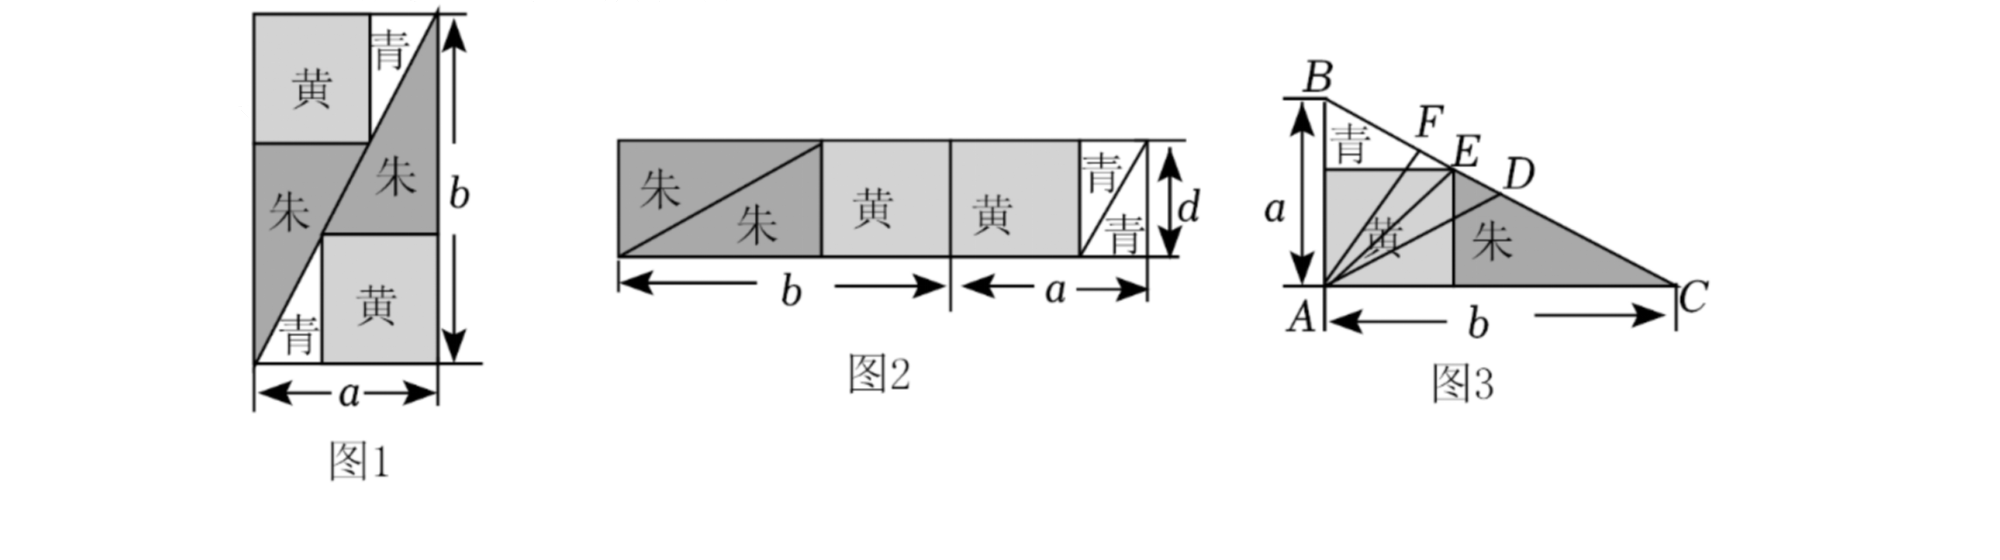
\includegraphics[width=0.86\textwidth]{figures/gao107_q11.png}
\end{center}

①由图 1 和图 2 面积相等得 $d=\dfrac{2ab}{a+b}$　　②由 $AE\geqslant AF$ 可得 $\sqrt{\dfrac{a^2+b^2}2}\geqslant\dfrac{a+b}2$

③由 $AD\geqslant AE$ 可得 $\sqrt{\dfrac{a^2+b^2}2}\geqslant\dfrac{2}{\dfrac1a+\dfrac1b}$　④由 $AD\geqslant AF$ 可得 $a^2+b^2\geqslant2ab$

\ifanswer
\solbegin
\step{对于①，由图 1 和图 2 面积相等得 $ab=(a+b)\times d$，所以 $d=\dfrac{ab}{a+b}$，故①错,}
\step{对于②，因为 $AF\perp BC$，所以 $\dfrac12ab=\dfrac12\sqrt{a^2+b^2}\times AF$,}
\step{所以 $AF=\dfrac{ab}{\sqrt{a^2+b^2}}$，$AE=\sqrt2d=\dfrac{\sqrt2ab}{a+b}$,}
\step{因为 $AE\geqslant AF$，所以 $\dfrac{\sqrt2ab}{a+b}\geqslant\dfrac{ab}{\sqrt{a^2+b^2}}$，整理得 $\sqrt{\dfrac{a^2+b^2}2}\geqslant\dfrac{a+b}2$，故②对,}
\step{对于③，因为 $D$ 是斜边 $BC$ 的中点，所以 $AD=\sqrt{\dfrac{a^2+b^2}2}$,}
\step{因为 $AD\geqslant AE$，所以 $\sqrt{\dfrac{a^2+b^2}2}\geqslant\dfrac{\sqrt2ab}{a+b}$，整理得 $\sqrt{\dfrac{a^2+b^2}2}\geqslant\dfrac{2}{\dfrac1a+\dfrac1b}$，故③对,}
\step{对于④，因为 $AD\geqslant AF$，所以 $\sqrt{\dfrac{a^2+b^2}2}\geqslant\dfrac{ab}{\sqrt{a^2+b^2}}$，整理得 $a^2+b^2\geqslant2ab$,}
\step{故④对,}
\step{故正确的是②③④.}
\solend
\fi

\item 设 $a,b,c,d\in\R$ 且$\lvert a-b\rvert\leqslant2$,$\lvert c-d\rvert\leqslant2$,$\lvert a\rvert\leqslant3$,$\lvert c\rvert\leqslant3$，则 $\lvert ad-bc\rvert$ 的最大值为\blankline[4.4em].% 原卷四处条件间均排半角逗号，照录

\ifanswer
\solbegin
\step{令 $a-b=e$,$c-d=f$，则 $\lvert e\rvert\leqslant2$,$\lvert f\rvert\leqslant2$,$\lvert a\rvert\leqslant3$,$\lvert c\rvert\leqslant3$}
\step{则 $\lvert ad-bc\rvert=\lvert a(c-f)-(a-e)c\rvert=\lvert ce-af\rvert\leqslant\lvert c\rvert\,\lvert e\rvert+\lvert a\rvert\,\lvert f\rvert\leqslant12$,}
\step{则 $\lvert ad-bc\rvert$ 的最大值为 12.}
\solend
\fi

\end{enumerate}

\bigsec{二、选择题}

\begin{enumerate}
\setcounter{enumi}{12}

\item 下列说法正确的是\mbox{（\quad）}

\keepwithprev
A. 若 $a>b>0$，则 $ac^2>bc^2$\qquad\qquad B. 若 $a<b<0$，则 $a^2>ab>b^2$

C. 若 $a>b$，则 $a^2>b^2$\qquad\qquad\qquad D. 若 $a<b$，则 $\dfrac1a>\dfrac1b$

\ifanswer
\solbegin
\step{$A$. 当 $a>b>0$ 时，取 $c=0$，则 $ac^2>bc^2$ 不成立，故 $A$ 错误；}
\step{$B$. 当 $a<b<0$ 时，由不等式的基本性质得 $a^2>ab>b^2>0$，故 $B$ 正确；}
\step{$C$. 当 $a>b$ 时，取 $a=0$，$b=-1$，则 $a^2>b^2$ 不成立，故 $C$ 错误；}
\step{$D$. 当 $a<b$ 时，取 $a=0$，$b=1$，则 $\dfrac1a>\dfrac1b$ 不成立，故 $D$ 错误.}
\step{故选 $B$.}
\solend
\fi

\item 小玲在学习《论语·子路》读到“其身正，不令而行；其身不正，虽令不从”，这句话的
数学含义可以理解为：“身正”是“令行”的\mbox{（\quad）}

\keepwithprev
A. 充分非必要条件\qquad\qquad B. 必要不充分条件

C. 充要条件\qquad\qquad\qquad D. 既非充分又非必要条件

\ifanswer
\solbegin
\step{其身正，不令而行，即身正$\Rightarrow$令行，所以“身正”是“令行”的充分条件；}
\step{又其身不正，虽令不从，即令行$\Rightarrow$身正，所以“身正”是“令行”的必要条件；}
\step{综上，“身正”是“令行”的充要条件. 故选 $C$.}
\solend
\fi

\item 某地对农户抽样调查，结果如下：电冰箱拥有率为 $45\%$，电视机拥有率为 $55\%$，洗衣
机拥有率为 $65\%$，拥有上述三种电器的任意两种的占 $35\%$，三种电器齐全的为 $25\%$，那
么一种电器也没有的农户所占比例是\mbox{（\quad）}

\keepwithprev
A. $12\%$\qquad B. $15\%$\qquad C. $18\%$\qquad D. $20\%$

\ifanswer
\solbegin
\step{设只有电冰箱和电视机的农户有 $a$ 家，只有电冰箱和洗衣机的农户有 $b$ 家,}
\step{只有洗衣机和电视机的农户有 $c$ 家,}
\step{只有电视机、电冰箱、洗衣机的分别有 $d$、$e$、$f$ 家,}
\step{没有任何电器的农户有 $x$ 家,}

\begin{center}
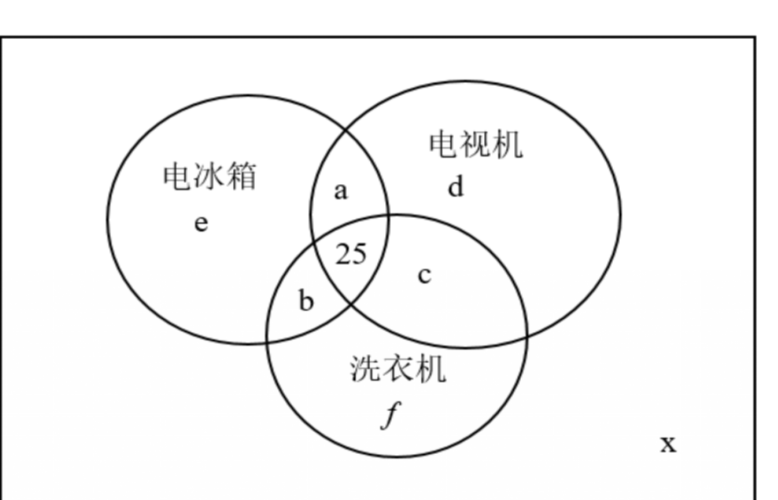
\includegraphics[width=0.42\textwidth]{figures/gao107_q15.png}
\end{center}

\step{所以 $25+a+b+e=45$①，$25+a+c+d=55$②,}
\step{$25+b+c+f=65$③,}
\step{把上面三个式子相加得 $2(a+b+c)+d+e+f=90$④,}
\step{对于拥有上述三种电器的任意两种的占 $35\%$，得 $a+b+c=35$⑤,}
\step{把⑤代入④可得到 $d+e+f=20$⑥,}
\step{因为农户共有 100 家，所以 $25+a+b+c+d+e+f+x=100$,}
\step{把⑤和⑥代入上式得 $x=20$，即一种电器也没有的农户所占比例为 $20\%$.}
\step{故选 $D$.}
\solend
\fi

\item 设 $d>0$，已知 $A,B$ 是两个数集. 若对任意 $x\in A$，都存在 $y\in B$，使得 $\lvert x-y\rvert<d$，则
称 $A$ 是 $B$ 的一个“$d-$邻集”. 现有下列两个命题：① $M=\{a+b\sqrt2\mid a,b\in\Z\}$ 是 $\Q$ 的一个
$\dfrac1{2025}$
一邻集；②若 $A$ 是 $B$ 的一个 $d-$邻集，则 $B$ 也是 $A$ 的一个 $d-$邻集；则\mbox{（\quad）}% 原卷把 d−邻集 的连字符断行后排成“一邻集”，照录

\keepwithprev
A. ①真②假\qquad B. ①假②真\qquad C. ①真②真\qquad D. ①假②假

\ifanswer
\solbegin
\step{对于①，任取 $M$ 中的元素 $x_0=a_0+b_0\sqrt2$,}
\step{则存在 $y_0\in\Q\cap\left(a_0+b_0\sqrt2-\dfrac1{2025},a_0+b_0\sqrt2+\dfrac1{2025}\right)$ 满足题意，故①正确；}
\step{对于②，取 $A=[-1,1]$,$B=[-2,2]$, $A$ 是 $B$ 的 $\dfrac12-$邻集，但反之不成立,}
\step{故②错误；}
\step{故选 $A$.}
\solend
\fi

\end{enumerate}

\bigsec{三、解答题}

\begin{enumerate}
\setcounter{enumi}{16}

\item 设 $a\in\R$，完成下列问题：

（1）求不等式 $3(a+1)x-3>2ax-3a$ 的解集 $M$；

（2）设集合 $A=\{x\mid x^2-ax+a^2-19=0\}$，$B=\{x\mid x^2-5x+6=0\}$，
$C=\{x\mid x^2+2x-8=0\}$. 若 $A\cap B\supset\varnothing$，$A\cap C=\varnothing$，求 $a$ 的值.

\ifanswer
\solbegin
\step{（1）不等式 $3(a+1)x-3>2ax-3a$ 可化为 $(a+3)x>3-3a$,}
\step{当 $a+3>0$，即 $a>-3$ 时，解得 $x>\dfrac{3-3a}{a+3}$,}
\step{当 $a+3=0$，即 $a=-3$ 时，不等式化为 $0\cdot x>12$，无解,}
\step{当 $a+3<0$，即 $a<-3$ 时，解得 $x<\dfrac{3-3a}{a+3}$,}
\step{综上所述，当 $a>-3$ 时，$M=\left(\dfrac{3-3a}{a+3},+\infty\right)$；}
\step{当 $a=-3$ 时，$M=\varnothing$；}
\step{当 $a<-3$ 时，$M=\left(-\infty,\dfrac{3-3a}{a+3}\right)$；}
\step{（2）$B=\{x\mid x^2-5x+6=0\}=\{2,3\}$，$C=\{x\mid x^2+2x-8=0\}=\{2,-4\}$,}
\step{因为 $A\cap B\supset\varnothing$，所以 $A\cap B\neq\varnothing$，又因为 $A\cap C=\varnothing$,}
\step{所以 $3\in A$，$2\notin A$，$-4\notin A$,}
\step{把 $x=3$ 代入方程 $x^2-ax+a^2-19=0$ 得 $9-3a+a^2-19=0$,}
\step{解得 $a=-2$ 或 $a=5$,}
\step{当 $a=-2$ 时，集合 $A=\{x\mid x^2+2x-15=0\}=\{3,-5\}$，符合题意,}
\step{当 $a=5$ 时，集合 $A=\{x\mid x^2-5x+6=0\}=\{3,2\}$，不符合题意，舍去,}
\step{综上所述，$a$ 的值为 $-2$.}
\solend
\fi

\item 完成下列问题：

（1）设 $x$、$y\in\R$，且 $x+y>5$，用反证法证明：$x>3$ 或 $y>2$；

（2）设 $x>0$，$a=x+1$，$b=\sqrt{x^2+7x+1}$，求 $\dfrac ba$ 的最大值.

\ifanswer
\solbegin
\step{（1）假设 $x\leqslant3$ 且 $y\leqslant2$，则 $x+y\leqslant3+2=5$，这与已知 $x+y>5$ 矛盾,}
\step{故 $x>3$ 或 $y>2$；}
\step{（2）$x>0$，$a=x+1$，$b=\sqrt{x^2+7x+1}$,}
\step{则 $\dfrac ba=\dfrac{\sqrt{x^2+7x+1}}{x+1}=\sqrt{\dfrac{x^2+7x+1}{x^2+2x+1}}=\sqrt{\dfrac{x^2+2x+1+5x}{x^2+2x+1}}$}
\step{$=\sqrt{1+\dfrac{5x}{x^2+2x+1}}=\sqrt{1+\dfrac{5}{x+\dfrac1x+2}}\leqslant\sqrt{1+\dfrac{5}{2\sqrt{x\cdot\dfrac1x}+2}}=\dfrac32$,}
\step{当且仅当 $x=\dfrac1x$，即 $x=1$ 时取等号，故 $\dfrac ba$ 的最大值为 $\dfrac32$.}
\solend
\fi

\item 已知函数 $f(x)=\lvert2x-a\rvert+a$.

（1）当 $a=2$ 时，求不等式 $f(x)\leqslant6+\lvert x+2\rvert$ 的解集；

（2）设 $g(x)=\lvert2x-1\rvert$，若不等式 $f(x)+g(x)\geqslant3$ 对一切 $x\in\R$ 恒成立，求实数 $a$ 的取值
范围.

\ifanswer
\solbegin
\ansspace*
\step{（1）$a=2$ 时，$f(x)=\lvert2x-2\rvert+2$,}
\step{则 $f(x)\leqslant6+\lvert x+2\rvert\Leftrightarrow\lvert2x-2\rvert+2\leqslant6+\lvert x+2\rvert$，即 $\lvert2x-2\rvert-\lvert x+2\rvert\leqslant4$,}
\step{当 $x<-2$ 时，$2-2x+x+2\leqslant4$，解得 $x\geqslant0$，与 $x<-2$ 取交集得 $\varnothing$,}
\step{当 $-2\leqslant x\leqslant1$ 时，$2-2x-x-2\leqslant4$，解得 $x\geqslant-\dfrac43$,}
\step{与 $-2\leqslant x\leqslant1$ 取交集得 $-\dfrac43\leqslant x\leqslant1$,}
\step{当 $x>1$ 时，$2x-2-x-2\leqslant4$，解得 $x\leqslant8$，与 $x>1$ 取交集得 $1<x\leqslant8$,}
\step{综上，不等式 $f(x)\leqslant6+\lvert x+2\rvert$ 的解集为 $\left\{x\,\middle|\,-\dfrac43\leqslant x\leqslant8\right\}$；}
\step{（2）$f(x)+g(x)\geqslant3$，即 $\lvert2x-a\rvert+a+\lvert2x-1\rvert\geqslant3$,}
\step{故 $\lvert2x-a\rvert+\lvert2x-1\rvert\geqslant3-a$,}
\step{当 $a\geqslant3$ 时，不等式显然成立,}
\step{当 $a<3$ 时,}
\step{由三角不等式得 $\lvert2x-a\rvert+\lvert2x-1\rvert\geqslant\lvert2x-a-(2x-1)\rvert=\lvert1-a\rvert$,}
\step{当且仅当 $(2x-a)(2x-1)\leqslant0$ 时取等号，因此 $\lvert1-a\rvert\geqslant3-a$,}
\step{平方得 $(1-a)^2\geqslant(3-a)^2$，解得 $a\geqslant2$，故 $2\leqslant a<3$.}
\step{综上，实数 $a$ 的取值范围是 $a\geqslant2$.}
\solend
\fi

\item 对于集合 $A,B$，定义集合 $A-B=\{x\mid x\in A$ 且 $x\notin B\}$.

（1）若 $A=\{1,2,3,4\}$,$B=\{3,4,5\}$，求集合 $A-B$ 和 $B-A$；

（2）给定集合 $A,B$，求所有满足方程组
\[
\begin{cases}
X\cap(A\cup B)=X\\
A\cap(B\cup X)=A\\
B\cap(A\cup X)=B\\
X\cap(A\cap B)=\varnothing
\end{cases}
\]
的集合 $X$（用 $A,B$ 表示）；

（3）用 $\lvert M\rvert$ 表示集合 $M$ 中的元素个数. 给定正整数 $n$，集合 $S=\{1,2,\cdots,n\}$. 对于实数
集的非空有限子集 $A,B$，定义集合 $C=\{x\mid x=a+b,a\in A,b\in B\}$. 求证：

$\lvert A-S\rvert+\lvert B-S\rvert+\lvert S-C\rvert\geqslant1$.

\ifanswer
\solbegin
\step{（1）由 $A=\{1,2,3,4\}$,$B=\{3,4,5\}$，则 $A-B=\{1,2\}$,$B-A=\{5\}$；}
\step{（2）由
$\begin{cases}
X\cap(A\cup B)=X\\
X\cap(A\cap B)=\varnothing
\end{cases}$，
得 $X\subseteq A-B$ 或 $X\subseteq B-A$,}
\step{再结合
$\begin{cases}
A\cap(B\cup X)=A\\
B\cap(A\cup X)=B
\end{cases}$，
得 $X=(A-B)\cup(B-A)$,}
\step{所以 $X=(A-B)\cup(B-A)$；}
\step{（3）$\lvert X\rvert$ 表示集合 $X$ 中的元素个数，则 $\lvert X\rvert\geqslant0$,}
\step{若 $A\cup B$ 中至少含有一个不在 $S$ 中的元素，则 $\lvert A-S\rvert+\lvert B-S\rvert\geqslant1$,}
\step{即 $\lvert A-S\rvert+\lvert B-S\rvert+\lvert S-C\rvert\geqslant1$.}
\step{若 $A\subseteq S$，且 $B\subseteq S$，则 $\lvert A-S\rvert=\lvert B-S\rvert=0$.}
\step{此时 $A$ 中最小的元素 $a\geqslant1$,$B$ 中最小的元素 $b\geqslant1$.}
\step{所以 $C$ 中最小的元素 $a+b\geqslant2$，则 $1\notin C$,}
\step{因为 $S=\{1,2,\cdots,n\}$，所以 $\lvert S-C\rvert\geqslant1$，即 $\lvert A-S\rvert+\lvert B-S\rvert+\lvert S-C\rvert\geqslant1$.}
\step{综上所述，$\lvert A-S\rvert+\lvert B-S\rvert+\lvert S-C\rvert\geqslant1$.}
\solend
\fi

\end{enumerate}

\end{document}
"
% 紧凑版：xelatex "\def\iscompact{1}% 高一107_曹杨二中_10月月考.tex
%   —— 高一上数学“2026-2027 年曹杨二中高一上 10 月月考”（试卷版/答案版）
% 试卷版：xelatex 高一107_曹杨二中_10月月考.tex
% 答案版：xelatex "\def\isanswer{1}% 高一107_曹杨二中_10月月考.tex
%   —— 高一上数学“2026-2027 年曹杨二中高一上 10 月月考”（试卷版/答案版）
% 试卷版：xelatex 高一107_曹杨二中_10月月考.tex
% 答案版：xelatex "\def\isanswer{1}\input{高一107_曹杨二中_10月月考.tex}"
% 紧凑版：xelatex "\def\iscompact{1}\input{高一107_曹杨二中_10月月考.tex}"
%
% 原始材料：微信公众号“魔都数学加油站”文章，作者破晓，2026-11-03 17:19 发布；
% 连载“27学年高一107”，原文标题“27学年高一107——2026-2027年上海市曹杨二中高一上10月月考”；
% 原文链接：https://mp.weixin.qq.com/s/IF4uB7aDNv-snYwbGMoDiQ。
% 正文为 10 张 PNG 页（第 1、2、4、6—9 页 4762×6735，第 3、5、10 页 2560×3620），题目下印有【解析】，为讲评版。
% 题目、解析均据原图转录；卷面水印及公众号页脚未录入。
% 第 11 题题干的三幅“出入相补”图（图 1—图 3）与第 15 题解析的三圆文氏图裁自原图、
% 去粉色水印转灰度（gao107_q11.png、gao107_q15.png），第 11 题图属题干（三版都出）、
% 第 15 题图属解析（仅答案版显示）。
%
% 卷首标题：原卷印作“2026-2027 年曹杨二中高一上 10 月月考”（公众号标题中的“上海市”
% 卷面标题行没有，本稿照卷面），年份区间按全稿惯例排 en dash；原卷未印副标题，本稿按题目内容
% 标为“集合与常用逻辑用语、不等式”。
%
% 与原卷的排版差异：
%   ① 原文从第 3 题起，填空题编号为 3—12、选择题为 13—16、解答题为 17—20，本稿保留原题号；
%   ② 原卷每题下直接印【解析】，本稿按全稿惯例将解析置于答案版；第 4 题只印【答案】另提 \ans{}；
%   ③ 原卷未印副标题，本稿按“知识模块”口径补出；
%   ④ 原卷填空横线按全稿惯例排为 \blankline[4.4em]；解答题按惯例加 \ansspace；选择题括号排
%      \mbox{（\quad）}、选项段前按惯例加 \keepwithprev；
%   ⑤ 原卷数集字母粗体与斜体混用（第 3 题 $\mathbf{R}$、第 4 题斜体 $R$、第 16 题粗体
%      $\mathbf{Z}$、$\mathbf{Q}$ 等），按全稿惯例统一改 \R、\Z、\Q。
%
% 原卷存疑：第 10 题解析“由 $\Delta=16m^2-8(2m^2+3m-2)\geqslant0$ 得 $m\leqslant\dfrac23$”
% 行末原卷无句读，照录。第 16 题解析②“取 $A=[-1,1]$，$B=[-2,2]$，$A$ 是 $B$ 的
% $\dfrac12$-邻集，但反之不成立”，据以判①真②假，照录。
%
% 行数核对：逐题数 \step/\stepm 条数，合计 112 条（Q3：5；Q4：0；Q5：2；Q6：2；Q7：2；
% Q8：4；Q9：8；Q10：4；Q11：9；Q12：3；Q13：5；Q14：3；Q15：12；Q16：5；Q17：15；
% Q18：6；Q19：15；Q20：12），与原卷印刷行逐题相等。第 4 题只印【答案】，提 \ans{}，
% 不计入 \step 账。
%
\documentclass[a4paper,11pt]{article}
\usepackage{common}

\begin{document}

\examtitlest[3]{2026--2027 年曹杨二中高一上 10 月月考}{集合与常用逻辑用语、不等式}

\bigsec{一、填空题}

\begin{enumerate}
\setcounter{enumi}{2}

\item 设 $a\in\R$，若 $3\in\{\sqrt3,a^2,a\}$，则 $a=$\blankline[4.4em].

\ifanswer
\solbegin
\step{因为 $3\in\{\sqrt3,a^2,a\}$，所以 $a^2=3$，解得 $a=\sqrt3$ 或 $a=-\sqrt3$,}
\step{当 $a=\sqrt3$ 时，集合为 $\{\sqrt3,3,\sqrt3\}$，不满足集合元素的互异性，舍去；}
\step{当 $a=-\sqrt3$ 时，集合为 $\{\sqrt3,3,-\sqrt3\}$，符合要求；}
\step{若 $a=3$，此时集合为 $\{\sqrt3,9,3\}$，符合要求；}
\step{综上，$a$ 为 $-\sqrt3$ 或 $3$.}
\solend
\fi

\item 设 $a\in\R$，已知集合 $A=\{x\mid x\leqslant a\}$，$B=\{x\mid x>2\}$. 若 $A\cup B=\R$，则 $a$ 的取值范围是\blankline[4.4em].

\ifanswer
\ans{$a\geqslant2$}
\fi

\item 设 $x>0$，$y>0$ 且 $x+3y=1$，则 $xy$ 的最大值为\blankline[4.4em].

\ifanswer
\solbegin
\step{由于 $x>0$，$y>0$ 且 $x+3y=1$，则 $1=x+3y\geqslant2\sqrt{3xy}$，得 $xy\leqslant\dfrac1{12}$,}
\step{当且仅当 $x=3y=\dfrac12$ 时取等号，则 $xy$ 的最大值为 $\dfrac1{12}$.}
\solend
\fi

\item 设 $a\in\R$，若集合$\left\{x\,\middle|\,\dfrac{ax}{x-1}=x\right\}$有且仅有两个子集，则 $a=$\blankline[4.4em].

\ifanswer
\solbegin
\step{由 $\dfrac{ax}{x-1}=x$ 得 $ax=x(x-1)$，即 $x(x-a-1)=0$,}
\step{所以此方程有两个相等的（不等于 1）的实数根或有一根为 1，所以 $a=-1$ 或 $0$.}
\solend
\fi

\item 已知全集 $U=\{x\mid x^2-8x-20<0\}$，集合 $A=\{x\mid 1-x^2>0$ 且 $x<0\}$，则 $\overline A=$\blankline[4.4em].

\ifanswer
\solbegin
\step{$U=\{x\mid-2<x<10\}$，$A=\{x\mid-1<x<0\}$,}
\step{所以 $\overline A=\{x\mid-2<x\leqslant-1$ 或 $0\leqslant x<10\}$.}
\solend
\fi

\item 设 $a,b\in\R$，若不等式 $-x^2-ax+b\geqslant0$ 的解集为 $[-2,3]$，则不等式 $\lvert ax+b\rvert<5$ 的解集为\blankline[4.4em].

\ifanswer
\solbegin
\step{由不等式 $-x^2-ax+b\geqslant0$ 的解集为 $[-2,3]$,}
\step{得 $-2$、$3$ 是方程 $-x^2-ax+b=0$ 的两个根，所以 $a=-1$，$b=6$.}
\step{解不等式 $\lvert-x+6\rvert<5$，得 $-5<x-6<5$，解得 $1<x<11$,}
\step{即所求不等式的解集为 $(1,11)$.}
\solend
\fi

\item 某货运卡车以 $x$ 千米／时的速度匀速行驶 300 千米，按交通法规限制 $50\leqslant x\leqslant100$，假设
柴油的价格为每升 6 元，汽车每小时耗油 $\left(4+\dfrac{x^2}{420}\right)$ 升，司机工资为每小时 46 元. 则当
$x=$\blankline[4.4em]（千米／时），这次行车的总费用（油费与司机工资的总和）最低.

\ifanswer
\solbegin
\step{因为卡车行驶 300 千米，速度为 $x$ 千米／时,}
\step{因此总用时为 $t=\dfrac{300}{x}$ 小时，其中 $50\leqslant x\leqslant100$,}
\step{每小时油费为 $6\cdot\left(4+\dfrac{x^2}{420}\right)$ 元，每小时司机工资为 46 元，因}
\step{此每小时总支出为 $6\cdot\left(4+\dfrac{x^2}{420}\right)+46=70+\dfrac{x^2}{70}$ 元.}
\step{设全程总费用为 $y$，则 $y=\dfrac{300}{x}\cdot\left(70+\dfrac{x^2}{70}\right)=\dfrac{21000}{x}+\dfrac{30x}{7}$,}
\step{因为 $50\leqslant x\leqslant100$，$\dfrac{21000}{x}+\dfrac{30x}{7}\geqslant2\sqrt{\dfrac{21000}{x}\cdot\dfrac{30x}{7}}=600$,}
\step{当且仅当 $\dfrac{21000}{x}=\dfrac{30x}{7}$，即 $x=70$ 时取等号，且 $70\in[50,100]$,}
\step{因此当 $x=70$ 千米／时，行车的总费用（油费与司机工资的总和）最低.}
\solend
\fi

\item 设 $x_1$、$x_2$ 是关于 $x$ 的方程 $2x^2-4mx+2m^2+3m-2=0$ 的两个实数根，则 $x_1^2+x_2^2$ 的最小值为\blankline[4.4em].

\ifanswer
\solbegin
\step{由题意得 $x_1+x_2=2m$，$x_1x_2=m^2+\dfrac{3m}{2}-1$,}
\step{由 $\Delta=16m^2-8(2m^2+3m-2)\geqslant0$ 得 $m\leqslant\dfrac23$}
\step{所以 $x_1^2+x_1^2=(x_1+x_2)^2-2x_1x_2=4m^2-2m^2+3m+2=2m^2-3m+2$,% 原卷左端作 x_1²+x_1²，照录
}
\step{结合二次函数的性质得，当 $m=\dfrac23$ 时取得最小值 $\dfrac89$.}
\solend
\fi

\item 小玲在钻研《九章算术》中“勾股容方”问题“今有勾五步，股十二步，问勾中容方几
何？”时，发现魏晋时期数学家刘徽在其《九章算术注》中利用出入相补原理给出了这个
问题的一般解法：如图 1，用对角线将长和宽分别为 $b$ 和 $a$ 的矩形分成两个直角三角形，
每个直角三角形再分成一个内接正方形（黄）和两个小直角三角形（朱、青）. 将三种颜色
的图形进行重组，得到如图 2 所示的矩形，该矩形长为 $a+b$，宽为内接正方形的边长
$d$. 由刘徽构造的图形可以得到许多重要的结论，如图 3，设 $D$ 为斜边 $BC$ 的中点，作直
角三角形 $ABC$ 的内接正方形对角线 $AE$，过点 $A$ 作 $AF\perp BC$ 于点 $F$，则下列四个推理中
正确的序号是\blankline[4.4em].

\begin{center}
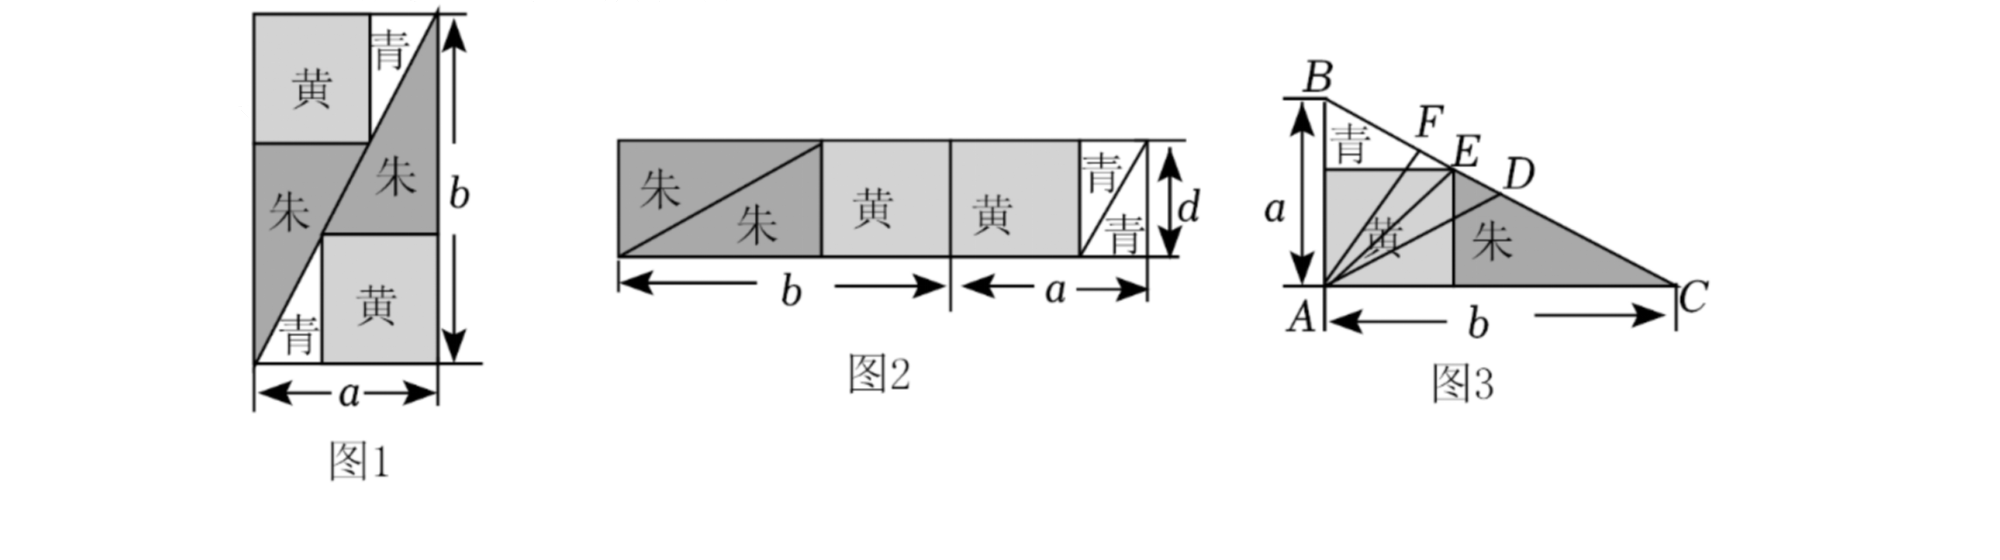
\includegraphics[width=0.86\textwidth]{figures/gao107_q11.png}
\end{center}

①由图 1 和图 2 面积相等得 $d=\dfrac{2ab}{a+b}$　　②由 $AE\geqslant AF$ 可得 $\sqrt{\dfrac{a^2+b^2}2}\geqslant\dfrac{a+b}2$

③由 $AD\geqslant AE$ 可得 $\sqrt{\dfrac{a^2+b^2}2}\geqslant\dfrac{2}{\dfrac1a+\dfrac1b}$　④由 $AD\geqslant AF$ 可得 $a^2+b^2\geqslant2ab$

\ifanswer
\solbegin
\step{对于①，由图 1 和图 2 面积相等得 $ab=(a+b)\times d$，所以 $d=\dfrac{ab}{a+b}$，故①错,}
\step{对于②，因为 $AF\perp BC$，所以 $\dfrac12ab=\dfrac12\sqrt{a^2+b^2}\times AF$,}
\step{所以 $AF=\dfrac{ab}{\sqrt{a^2+b^2}}$，$AE=\sqrt2d=\dfrac{\sqrt2ab}{a+b}$,}
\step{因为 $AE\geqslant AF$，所以 $\dfrac{\sqrt2ab}{a+b}\geqslant\dfrac{ab}{\sqrt{a^2+b^2}}$，整理得 $\sqrt{\dfrac{a^2+b^2}2}\geqslant\dfrac{a+b}2$，故②对,}
\step{对于③，因为 $D$ 是斜边 $BC$ 的中点，所以 $AD=\sqrt{\dfrac{a^2+b^2}2}$,}
\step{因为 $AD\geqslant AE$，所以 $\sqrt{\dfrac{a^2+b^2}2}\geqslant\dfrac{\sqrt2ab}{a+b}$，整理得 $\sqrt{\dfrac{a^2+b^2}2}\geqslant\dfrac{2}{\dfrac1a+\dfrac1b}$，故③对,}
\step{对于④，因为 $AD\geqslant AF$，所以 $\sqrt{\dfrac{a^2+b^2}2}\geqslant\dfrac{ab}{\sqrt{a^2+b^2}}$，整理得 $a^2+b^2\geqslant2ab$,}
\step{故④对,}
\step{故正确的是②③④.}
\solend
\fi

\item 设 $a,b,c,d\in\R$ 且$\lvert a-b\rvert\leqslant2$,$\lvert c-d\rvert\leqslant2$,$\lvert a\rvert\leqslant3$,$\lvert c\rvert\leqslant3$，则 $\lvert ad-bc\rvert$ 的最大值为\blankline[4.4em].% 原卷四处条件间均排半角逗号，照录

\ifanswer
\solbegin
\step{令 $a-b=e$,$c-d=f$，则 $\lvert e\rvert\leqslant2$,$\lvert f\rvert\leqslant2$,$\lvert a\rvert\leqslant3$,$\lvert c\rvert\leqslant3$}
\step{则 $\lvert ad-bc\rvert=\lvert a(c-f)-(a-e)c\rvert=\lvert ce-af\rvert\leqslant\lvert c\rvert\,\lvert e\rvert+\lvert a\rvert\,\lvert f\rvert\leqslant12$,}
\step{则 $\lvert ad-bc\rvert$ 的最大值为 12.}
\solend
\fi

\end{enumerate}

\bigsec{二、选择题}

\begin{enumerate}
\setcounter{enumi}{12}

\item 下列说法正确的是\mbox{（\quad）}

\keepwithprev
A. 若 $a>b>0$，则 $ac^2>bc^2$\qquad\qquad B. 若 $a<b<0$，则 $a^2>ab>b^2$

C. 若 $a>b$，则 $a^2>b^2$\qquad\qquad\qquad D. 若 $a<b$，则 $\dfrac1a>\dfrac1b$

\ifanswer
\solbegin
\step{$A$. 当 $a>b>0$ 时，取 $c=0$，则 $ac^2>bc^2$ 不成立，故 $A$ 错误；}
\step{$B$. 当 $a<b<0$ 时，由不等式的基本性质得 $a^2>ab>b^2>0$，故 $B$ 正确；}
\step{$C$. 当 $a>b$ 时，取 $a=0$，$b=-1$，则 $a^2>b^2$ 不成立，故 $C$ 错误；}
\step{$D$. 当 $a<b$ 时，取 $a=0$，$b=1$，则 $\dfrac1a>\dfrac1b$ 不成立，故 $D$ 错误.}
\step{故选 $B$.}
\solend
\fi

\item 小玲在学习《论语·子路》读到“其身正，不令而行；其身不正，虽令不从”，这句话的
数学含义可以理解为：“身正”是“令行”的\mbox{（\quad）}

\keepwithprev
A. 充分非必要条件\qquad\qquad B. 必要不充分条件

C. 充要条件\qquad\qquad\qquad D. 既非充分又非必要条件

\ifanswer
\solbegin
\step{其身正，不令而行，即身正$\Rightarrow$令行，所以“身正”是“令行”的充分条件；}
\step{又其身不正，虽令不从，即令行$\Rightarrow$身正，所以“身正”是“令行”的必要条件；}
\step{综上，“身正”是“令行”的充要条件. 故选 $C$.}
\solend
\fi

\item 某地对农户抽样调查，结果如下：电冰箱拥有率为 $45\%$，电视机拥有率为 $55\%$，洗衣
机拥有率为 $65\%$，拥有上述三种电器的任意两种的占 $35\%$，三种电器齐全的为 $25\%$，那
么一种电器也没有的农户所占比例是\mbox{（\quad）}

\keepwithprev
A. $12\%$\qquad B. $15\%$\qquad C. $18\%$\qquad D. $20\%$

\ifanswer
\solbegin
\step{设只有电冰箱和电视机的农户有 $a$ 家，只有电冰箱和洗衣机的农户有 $b$ 家,}
\step{只有洗衣机和电视机的农户有 $c$ 家,}
\step{只有电视机、电冰箱、洗衣机的分别有 $d$、$e$、$f$ 家,}
\step{没有任何电器的农户有 $x$ 家,}

\begin{center}
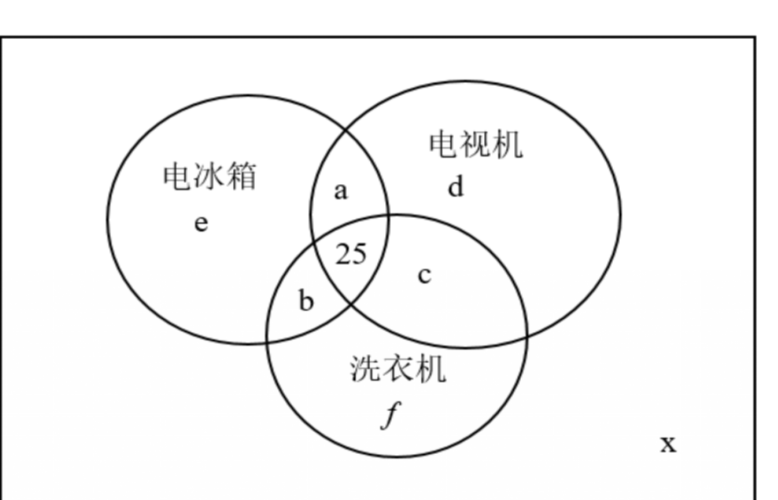
\includegraphics[width=0.42\textwidth]{figures/gao107_q15.png}
\end{center}

\step{所以 $25+a+b+e=45$①，$25+a+c+d=55$②,}
\step{$25+b+c+f=65$③,}
\step{把上面三个式子相加得 $2(a+b+c)+d+e+f=90$④,}
\step{对于拥有上述三种电器的任意两种的占 $35\%$，得 $a+b+c=35$⑤,}
\step{把⑤代入④可得到 $d+e+f=20$⑥,}
\step{因为农户共有 100 家，所以 $25+a+b+c+d+e+f+x=100$,}
\step{把⑤和⑥代入上式得 $x=20$，即一种电器也没有的农户所占比例为 $20\%$.}
\step{故选 $D$.}
\solend
\fi

\item 设 $d>0$，已知 $A,B$ 是两个数集. 若对任意 $x\in A$，都存在 $y\in B$，使得 $\lvert x-y\rvert<d$，则
称 $A$ 是 $B$ 的一个“$d-$邻集”. 现有下列两个命题：① $M=\{a+b\sqrt2\mid a,b\in\Z\}$ 是 $\Q$ 的一个
$\dfrac1{2025}$
一邻集；②若 $A$ 是 $B$ 的一个 $d-$邻集，则 $B$ 也是 $A$ 的一个 $d-$邻集；则\mbox{（\quad）}% 原卷把 d−邻集 的连字符断行后排成“一邻集”，照录

\keepwithprev
A. ①真②假\qquad B. ①假②真\qquad C. ①真②真\qquad D. ①假②假

\ifanswer
\solbegin
\step{对于①，任取 $M$ 中的元素 $x_0=a_0+b_0\sqrt2$,}
\step{则存在 $y_0\in\Q\cap\left(a_0+b_0\sqrt2-\dfrac1{2025},a_0+b_0\sqrt2+\dfrac1{2025}\right)$ 满足题意，故①正确；}
\step{对于②，取 $A=[-1,1]$,$B=[-2,2]$, $A$ 是 $B$ 的 $\dfrac12-$邻集，但反之不成立,}
\step{故②错误；}
\step{故选 $A$.}
\solend
\fi

\end{enumerate}

\bigsec{三、解答题}

\begin{enumerate}
\setcounter{enumi}{16}

\item 设 $a\in\R$，完成下列问题：

（1）求不等式 $3(a+1)x-3>2ax-3a$ 的解集 $M$；

（2）设集合 $A=\{x\mid x^2-ax+a^2-19=0\}$，$B=\{x\mid x^2-5x+6=0\}$，
$C=\{x\mid x^2+2x-8=0\}$. 若 $A\cap B\supset\varnothing$，$A\cap C=\varnothing$，求 $a$ 的值.

\ifanswer
\solbegin
\step{（1）不等式 $3(a+1)x-3>2ax-3a$ 可化为 $(a+3)x>3-3a$,}
\step{当 $a+3>0$，即 $a>-3$ 时，解得 $x>\dfrac{3-3a}{a+3}$,}
\step{当 $a+3=0$，即 $a=-3$ 时，不等式化为 $0\cdot x>12$，无解,}
\step{当 $a+3<0$，即 $a<-3$ 时，解得 $x<\dfrac{3-3a}{a+3}$,}
\step{综上所述，当 $a>-3$ 时，$M=\left(\dfrac{3-3a}{a+3},+\infty\right)$；}
\step{当 $a=-3$ 时，$M=\varnothing$；}
\step{当 $a<-3$ 时，$M=\left(-\infty,\dfrac{3-3a}{a+3}\right)$；}
\step{（2）$B=\{x\mid x^2-5x+6=0\}=\{2,3\}$，$C=\{x\mid x^2+2x-8=0\}=\{2,-4\}$,}
\step{因为 $A\cap B\supset\varnothing$，所以 $A\cap B\neq\varnothing$，又因为 $A\cap C=\varnothing$,}
\step{所以 $3\in A$，$2\notin A$，$-4\notin A$,}
\step{把 $x=3$ 代入方程 $x^2-ax+a^2-19=0$ 得 $9-3a+a^2-19=0$,}
\step{解得 $a=-2$ 或 $a=5$,}
\step{当 $a=-2$ 时，集合 $A=\{x\mid x^2+2x-15=0\}=\{3,-5\}$，符合题意,}
\step{当 $a=5$ 时，集合 $A=\{x\mid x^2-5x+6=0\}=\{3,2\}$，不符合题意，舍去,}
\step{综上所述，$a$ 的值为 $-2$.}
\solend
\fi

\item 完成下列问题：

（1）设 $x$、$y\in\R$，且 $x+y>5$，用反证法证明：$x>3$ 或 $y>2$；

（2）设 $x>0$，$a=x+1$，$b=\sqrt{x^2+7x+1}$，求 $\dfrac ba$ 的最大值.

\ifanswer
\solbegin
\step{（1）假设 $x\leqslant3$ 且 $y\leqslant2$，则 $x+y\leqslant3+2=5$，这与已知 $x+y>5$ 矛盾,}
\step{故 $x>3$ 或 $y>2$；}
\step{（2）$x>0$，$a=x+1$，$b=\sqrt{x^2+7x+1}$,}
\step{则 $\dfrac ba=\dfrac{\sqrt{x^2+7x+1}}{x+1}=\sqrt{\dfrac{x^2+7x+1}{x^2+2x+1}}=\sqrt{\dfrac{x^2+2x+1+5x}{x^2+2x+1}}$}
\step{$=\sqrt{1+\dfrac{5x}{x^2+2x+1}}=\sqrt{1+\dfrac{5}{x+\dfrac1x+2}}\leqslant\sqrt{1+\dfrac{5}{2\sqrt{x\cdot\dfrac1x}+2}}=\dfrac32$,}
\step{当且仅当 $x=\dfrac1x$，即 $x=1$ 时取等号，故 $\dfrac ba$ 的最大值为 $\dfrac32$.}
\solend
\fi

\item 已知函数 $f(x)=\lvert2x-a\rvert+a$.

（1）当 $a=2$ 时，求不等式 $f(x)\leqslant6+\lvert x+2\rvert$ 的解集；

（2）设 $g(x)=\lvert2x-1\rvert$，若不等式 $f(x)+g(x)\geqslant3$ 对一切 $x\in\R$ 恒成立，求实数 $a$ 的取值
范围.

\ifanswer
\solbegin
\ansspace*
\step{（1）$a=2$ 时，$f(x)=\lvert2x-2\rvert+2$,}
\step{则 $f(x)\leqslant6+\lvert x+2\rvert\Leftrightarrow\lvert2x-2\rvert+2\leqslant6+\lvert x+2\rvert$，即 $\lvert2x-2\rvert-\lvert x+2\rvert\leqslant4$,}
\step{当 $x<-2$ 时，$2-2x+x+2\leqslant4$，解得 $x\geqslant0$，与 $x<-2$ 取交集得 $\varnothing$,}
\step{当 $-2\leqslant x\leqslant1$ 时，$2-2x-x-2\leqslant4$，解得 $x\geqslant-\dfrac43$,}
\step{与 $-2\leqslant x\leqslant1$ 取交集得 $-\dfrac43\leqslant x\leqslant1$,}
\step{当 $x>1$ 时，$2x-2-x-2\leqslant4$，解得 $x\leqslant8$，与 $x>1$ 取交集得 $1<x\leqslant8$,}
\step{综上，不等式 $f(x)\leqslant6+\lvert x+2\rvert$ 的解集为 $\left\{x\,\middle|\,-\dfrac43\leqslant x\leqslant8\right\}$；}
\step{（2）$f(x)+g(x)\geqslant3$，即 $\lvert2x-a\rvert+a+\lvert2x-1\rvert\geqslant3$,}
\step{故 $\lvert2x-a\rvert+\lvert2x-1\rvert\geqslant3-a$,}
\step{当 $a\geqslant3$ 时，不等式显然成立,}
\step{当 $a<3$ 时,}
\step{由三角不等式得 $\lvert2x-a\rvert+\lvert2x-1\rvert\geqslant\lvert2x-a-(2x-1)\rvert=\lvert1-a\rvert$,}
\step{当且仅当 $(2x-a)(2x-1)\leqslant0$ 时取等号，因此 $\lvert1-a\rvert\geqslant3-a$,}
\step{平方得 $(1-a)^2\geqslant(3-a)^2$，解得 $a\geqslant2$，故 $2\leqslant a<3$.}
\step{综上，实数 $a$ 的取值范围是 $a\geqslant2$.}
\solend
\fi

\item 对于集合 $A,B$，定义集合 $A-B=\{x\mid x\in A$ 且 $x\notin B\}$.

（1）若 $A=\{1,2,3,4\}$,$B=\{3,4,5\}$，求集合 $A-B$ 和 $B-A$；

（2）给定集合 $A,B$，求所有满足方程组
\[
\begin{cases}
X\cap(A\cup B)=X\\
A\cap(B\cup X)=A\\
B\cap(A\cup X)=B\\
X\cap(A\cap B)=\varnothing
\end{cases}
\]
的集合 $X$（用 $A,B$ 表示）；

（3）用 $\lvert M\rvert$ 表示集合 $M$ 中的元素个数. 给定正整数 $n$，集合 $S=\{1,2,\cdots,n\}$. 对于实数
集的非空有限子集 $A,B$，定义集合 $C=\{x\mid x=a+b,a\in A,b\in B\}$. 求证：

$\lvert A-S\rvert+\lvert B-S\rvert+\lvert S-C\rvert\geqslant1$.

\ifanswer
\solbegin
\step{（1）由 $A=\{1,2,3,4\}$,$B=\{3,4,5\}$，则 $A-B=\{1,2\}$,$B-A=\{5\}$；}
\step{（2）由
$\begin{cases}
X\cap(A\cup B)=X\\
X\cap(A\cap B)=\varnothing
\end{cases}$，
得 $X\subseteq A-B$ 或 $X\subseteq B-A$,}
\step{再结合
$\begin{cases}
A\cap(B\cup X)=A\\
B\cap(A\cup X)=B
\end{cases}$，
得 $X=(A-B)\cup(B-A)$,}
\step{所以 $X=(A-B)\cup(B-A)$；}
\step{（3）$\lvert X\rvert$ 表示集合 $X$ 中的元素个数，则 $\lvert X\rvert\geqslant0$,}
\step{若 $A\cup B$ 中至少含有一个不在 $S$ 中的元素，则 $\lvert A-S\rvert+\lvert B-S\rvert\geqslant1$,}
\step{即 $\lvert A-S\rvert+\lvert B-S\rvert+\lvert S-C\rvert\geqslant1$.}
\step{若 $A\subseteq S$，且 $B\subseteq S$，则 $\lvert A-S\rvert=\lvert B-S\rvert=0$.}
\step{此时 $A$ 中最小的元素 $a\geqslant1$,$B$ 中最小的元素 $b\geqslant1$.}
\step{所以 $C$ 中最小的元素 $a+b\geqslant2$，则 $1\notin C$,}
\step{因为 $S=\{1,2,\cdots,n\}$，所以 $\lvert S-C\rvert\geqslant1$，即 $\lvert A-S\rvert+\lvert B-S\rvert+\lvert S-C\rvert\geqslant1$.}
\step{综上所述，$\lvert A-S\rvert+\lvert B-S\rvert+\lvert S-C\rvert\geqslant1$.}
\solend
\fi

\end{enumerate}

\end{document}
"
% 紧凑版：xelatex "\def\iscompact{1}% 高一107_曹杨二中_10月月考.tex
%   —— 高一上数学“2026-2027 年曹杨二中高一上 10 月月考”（试卷版/答案版）
% 试卷版：xelatex 高一107_曹杨二中_10月月考.tex
% 答案版：xelatex "\def\isanswer{1}\input{高一107_曹杨二中_10月月考.tex}"
% 紧凑版：xelatex "\def\iscompact{1}\input{高一107_曹杨二中_10月月考.tex}"
%
% 原始材料：微信公众号“魔都数学加油站”文章，作者破晓，2026-11-03 17:19 发布；
% 连载“27学年高一107”，原文标题“27学年高一107——2026-2027年上海市曹杨二中高一上10月月考”；
% 原文链接：https://mp.weixin.qq.com/s/IF4uB7aDNv-snYwbGMoDiQ。
% 正文为 10 张 PNG 页（第 1、2、4、6—9 页 4762×6735，第 3、5、10 页 2560×3620），题目下印有【解析】，为讲评版。
% 题目、解析均据原图转录；卷面水印及公众号页脚未录入。
% 第 11 题题干的三幅“出入相补”图（图 1—图 3）与第 15 题解析的三圆文氏图裁自原图、
% 去粉色水印转灰度（gao107_q11.png、gao107_q15.png），第 11 题图属题干（三版都出）、
% 第 15 题图属解析（仅答案版显示）。
%
% 卷首标题：原卷印作“2026-2027 年曹杨二中高一上 10 月月考”（公众号标题中的“上海市”
% 卷面标题行没有，本稿照卷面），年份区间按全稿惯例排 en dash；原卷未印副标题，本稿按题目内容
% 标为“集合与常用逻辑用语、不等式”。
%
% 与原卷的排版差异：
%   ① 原文从第 3 题起，填空题编号为 3—12、选择题为 13—16、解答题为 17—20，本稿保留原题号；
%   ② 原卷每题下直接印【解析】，本稿按全稿惯例将解析置于答案版；第 4 题只印【答案】另提 \ans{}；
%   ③ 原卷未印副标题，本稿按“知识模块”口径补出；
%   ④ 原卷填空横线按全稿惯例排为 \blankline[4.4em]；解答题按惯例加 \ansspace；选择题括号排
%      \mbox{（\quad）}、选项段前按惯例加 \keepwithprev；
%   ⑤ 原卷数集字母粗体与斜体混用（第 3 题 $\mathbf{R}$、第 4 题斜体 $R$、第 16 题粗体
%      $\mathbf{Z}$、$\mathbf{Q}$ 等），按全稿惯例统一改 \R、\Z、\Q。
%
% 原卷存疑：第 10 题解析“由 $\Delta=16m^2-8(2m^2+3m-2)\geqslant0$ 得 $m\leqslant\dfrac23$”
% 行末原卷无句读，照录。第 16 题解析②“取 $A=[-1,1]$，$B=[-2,2]$，$A$ 是 $B$ 的
% $\dfrac12$-邻集，但反之不成立”，据以判①真②假，照录。
%
% 行数核对：逐题数 \step/\stepm 条数，合计 112 条（Q3：5；Q4：0；Q5：2；Q6：2；Q7：2；
% Q8：4；Q9：8；Q10：4；Q11：9；Q12：3；Q13：5；Q14：3；Q15：12；Q16：5；Q17：15；
% Q18：6；Q19：15；Q20：12），与原卷印刷行逐题相等。第 4 题只印【答案】，提 \ans{}，
% 不计入 \step 账。
%
\documentclass[a4paper,11pt]{article}
\usepackage{common}

\begin{document}

\examtitlest[3]{2026--2027 年曹杨二中高一上 10 月月考}{集合与常用逻辑用语、不等式}

\bigsec{一、填空题}

\begin{enumerate}
\setcounter{enumi}{2}

\item 设 $a\in\R$，若 $3\in\{\sqrt3,a^2,a\}$，则 $a=$\blankline[4.4em].

\ifanswer
\solbegin
\step{因为 $3\in\{\sqrt3,a^2,a\}$，所以 $a^2=3$，解得 $a=\sqrt3$ 或 $a=-\sqrt3$,}
\step{当 $a=\sqrt3$ 时，集合为 $\{\sqrt3,3,\sqrt3\}$，不满足集合元素的互异性，舍去；}
\step{当 $a=-\sqrt3$ 时，集合为 $\{\sqrt3,3,-\sqrt3\}$，符合要求；}
\step{若 $a=3$，此时集合为 $\{\sqrt3,9,3\}$，符合要求；}
\step{综上，$a$ 为 $-\sqrt3$ 或 $3$.}
\solend
\fi

\item 设 $a\in\R$，已知集合 $A=\{x\mid x\leqslant a\}$，$B=\{x\mid x>2\}$. 若 $A\cup B=\R$，则 $a$ 的取值范围是\blankline[4.4em].

\ifanswer
\ans{$a\geqslant2$}
\fi

\item 设 $x>0$，$y>0$ 且 $x+3y=1$，则 $xy$ 的最大值为\blankline[4.4em].

\ifanswer
\solbegin
\step{由于 $x>0$，$y>0$ 且 $x+3y=1$，则 $1=x+3y\geqslant2\sqrt{3xy}$，得 $xy\leqslant\dfrac1{12}$,}
\step{当且仅当 $x=3y=\dfrac12$ 时取等号，则 $xy$ 的最大值为 $\dfrac1{12}$.}
\solend
\fi

\item 设 $a\in\R$，若集合$\left\{x\,\middle|\,\dfrac{ax}{x-1}=x\right\}$有且仅有两个子集，则 $a=$\blankline[4.4em].

\ifanswer
\solbegin
\step{由 $\dfrac{ax}{x-1}=x$ 得 $ax=x(x-1)$，即 $x(x-a-1)=0$,}
\step{所以此方程有两个相等的（不等于 1）的实数根或有一根为 1，所以 $a=-1$ 或 $0$.}
\solend
\fi

\item 已知全集 $U=\{x\mid x^2-8x-20<0\}$，集合 $A=\{x\mid 1-x^2>0$ 且 $x<0\}$，则 $\overline A=$\blankline[4.4em].

\ifanswer
\solbegin
\step{$U=\{x\mid-2<x<10\}$，$A=\{x\mid-1<x<0\}$,}
\step{所以 $\overline A=\{x\mid-2<x\leqslant-1$ 或 $0\leqslant x<10\}$.}
\solend
\fi

\item 设 $a,b\in\R$，若不等式 $-x^2-ax+b\geqslant0$ 的解集为 $[-2,3]$，则不等式 $\lvert ax+b\rvert<5$ 的解集为\blankline[4.4em].

\ifanswer
\solbegin
\step{由不等式 $-x^2-ax+b\geqslant0$ 的解集为 $[-2,3]$,}
\step{得 $-2$、$3$ 是方程 $-x^2-ax+b=0$ 的两个根，所以 $a=-1$，$b=6$.}
\step{解不等式 $\lvert-x+6\rvert<5$，得 $-5<x-6<5$，解得 $1<x<11$,}
\step{即所求不等式的解集为 $(1,11)$.}
\solend
\fi

\item 某货运卡车以 $x$ 千米／时的速度匀速行驶 300 千米，按交通法规限制 $50\leqslant x\leqslant100$，假设
柴油的价格为每升 6 元，汽车每小时耗油 $\left(4+\dfrac{x^2}{420}\right)$ 升，司机工资为每小时 46 元. 则当
$x=$\blankline[4.4em]（千米／时），这次行车的总费用（油费与司机工资的总和）最低.

\ifanswer
\solbegin
\step{因为卡车行驶 300 千米，速度为 $x$ 千米／时,}
\step{因此总用时为 $t=\dfrac{300}{x}$ 小时，其中 $50\leqslant x\leqslant100$,}
\step{每小时油费为 $6\cdot\left(4+\dfrac{x^2}{420}\right)$ 元，每小时司机工资为 46 元，因}
\step{此每小时总支出为 $6\cdot\left(4+\dfrac{x^2}{420}\right)+46=70+\dfrac{x^2}{70}$ 元.}
\step{设全程总费用为 $y$，则 $y=\dfrac{300}{x}\cdot\left(70+\dfrac{x^2}{70}\right)=\dfrac{21000}{x}+\dfrac{30x}{7}$,}
\step{因为 $50\leqslant x\leqslant100$，$\dfrac{21000}{x}+\dfrac{30x}{7}\geqslant2\sqrt{\dfrac{21000}{x}\cdot\dfrac{30x}{7}}=600$,}
\step{当且仅当 $\dfrac{21000}{x}=\dfrac{30x}{7}$，即 $x=70$ 时取等号，且 $70\in[50,100]$,}
\step{因此当 $x=70$ 千米／时，行车的总费用（油费与司机工资的总和）最低.}
\solend
\fi

\item 设 $x_1$、$x_2$ 是关于 $x$ 的方程 $2x^2-4mx+2m^2+3m-2=0$ 的两个实数根，则 $x_1^2+x_2^2$ 的最小值为\blankline[4.4em].

\ifanswer
\solbegin
\step{由题意得 $x_1+x_2=2m$，$x_1x_2=m^2+\dfrac{3m}{2}-1$,}
\step{由 $\Delta=16m^2-8(2m^2+3m-2)\geqslant0$ 得 $m\leqslant\dfrac23$}
\step{所以 $x_1^2+x_1^2=(x_1+x_2)^2-2x_1x_2=4m^2-2m^2+3m+2=2m^2-3m+2$,% 原卷左端作 x_1²+x_1²，照录
}
\step{结合二次函数的性质得，当 $m=\dfrac23$ 时取得最小值 $\dfrac89$.}
\solend
\fi

\item 小玲在钻研《九章算术》中“勾股容方”问题“今有勾五步，股十二步，问勾中容方几
何？”时，发现魏晋时期数学家刘徽在其《九章算术注》中利用出入相补原理给出了这个
问题的一般解法：如图 1，用对角线将长和宽分别为 $b$ 和 $a$ 的矩形分成两个直角三角形，
每个直角三角形再分成一个内接正方形（黄）和两个小直角三角形（朱、青）. 将三种颜色
的图形进行重组，得到如图 2 所示的矩形，该矩形长为 $a+b$，宽为内接正方形的边长
$d$. 由刘徽构造的图形可以得到许多重要的结论，如图 3，设 $D$ 为斜边 $BC$ 的中点，作直
角三角形 $ABC$ 的内接正方形对角线 $AE$，过点 $A$ 作 $AF\perp BC$ 于点 $F$，则下列四个推理中
正确的序号是\blankline[4.4em].

\begin{center}
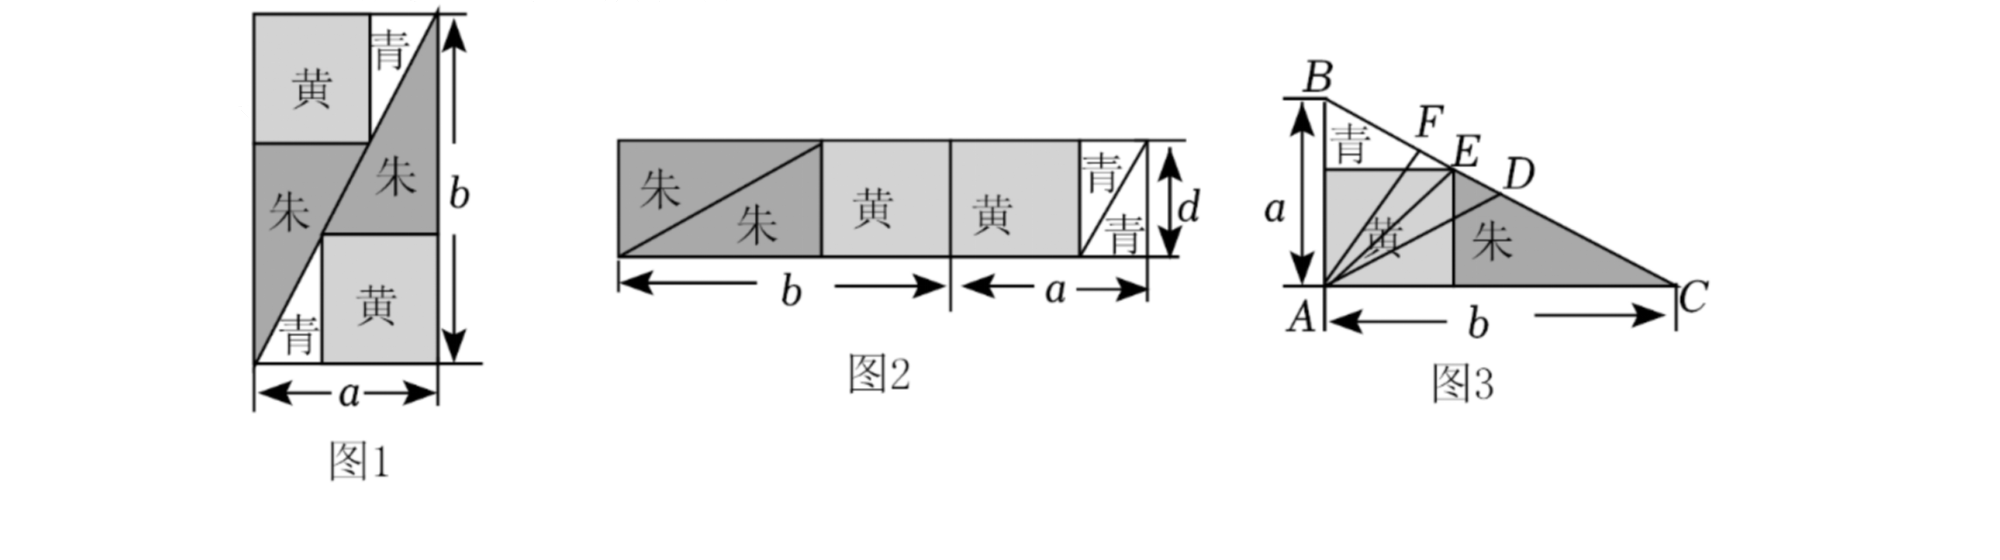
\includegraphics[width=0.86\textwidth]{figures/gao107_q11.png}
\end{center}

①由图 1 和图 2 面积相等得 $d=\dfrac{2ab}{a+b}$　　②由 $AE\geqslant AF$ 可得 $\sqrt{\dfrac{a^2+b^2}2}\geqslant\dfrac{a+b}2$

③由 $AD\geqslant AE$ 可得 $\sqrt{\dfrac{a^2+b^2}2}\geqslant\dfrac{2}{\dfrac1a+\dfrac1b}$　④由 $AD\geqslant AF$ 可得 $a^2+b^2\geqslant2ab$

\ifanswer
\solbegin
\step{对于①，由图 1 和图 2 面积相等得 $ab=(a+b)\times d$，所以 $d=\dfrac{ab}{a+b}$，故①错,}
\step{对于②，因为 $AF\perp BC$，所以 $\dfrac12ab=\dfrac12\sqrt{a^2+b^2}\times AF$,}
\step{所以 $AF=\dfrac{ab}{\sqrt{a^2+b^2}}$，$AE=\sqrt2d=\dfrac{\sqrt2ab}{a+b}$,}
\step{因为 $AE\geqslant AF$，所以 $\dfrac{\sqrt2ab}{a+b}\geqslant\dfrac{ab}{\sqrt{a^2+b^2}}$，整理得 $\sqrt{\dfrac{a^2+b^2}2}\geqslant\dfrac{a+b}2$，故②对,}
\step{对于③，因为 $D$ 是斜边 $BC$ 的中点，所以 $AD=\sqrt{\dfrac{a^2+b^2}2}$,}
\step{因为 $AD\geqslant AE$，所以 $\sqrt{\dfrac{a^2+b^2}2}\geqslant\dfrac{\sqrt2ab}{a+b}$，整理得 $\sqrt{\dfrac{a^2+b^2}2}\geqslant\dfrac{2}{\dfrac1a+\dfrac1b}$，故③对,}
\step{对于④，因为 $AD\geqslant AF$，所以 $\sqrt{\dfrac{a^2+b^2}2}\geqslant\dfrac{ab}{\sqrt{a^2+b^2}}$，整理得 $a^2+b^2\geqslant2ab$,}
\step{故④对,}
\step{故正确的是②③④.}
\solend
\fi

\item 设 $a,b,c,d\in\R$ 且$\lvert a-b\rvert\leqslant2$,$\lvert c-d\rvert\leqslant2$,$\lvert a\rvert\leqslant3$,$\lvert c\rvert\leqslant3$，则 $\lvert ad-bc\rvert$ 的最大值为\blankline[4.4em].% 原卷四处条件间均排半角逗号，照录

\ifanswer
\solbegin
\step{令 $a-b=e$,$c-d=f$，则 $\lvert e\rvert\leqslant2$,$\lvert f\rvert\leqslant2$,$\lvert a\rvert\leqslant3$,$\lvert c\rvert\leqslant3$}
\step{则 $\lvert ad-bc\rvert=\lvert a(c-f)-(a-e)c\rvert=\lvert ce-af\rvert\leqslant\lvert c\rvert\,\lvert e\rvert+\lvert a\rvert\,\lvert f\rvert\leqslant12$,}
\step{则 $\lvert ad-bc\rvert$ 的最大值为 12.}
\solend
\fi

\end{enumerate}

\bigsec{二、选择题}

\begin{enumerate}
\setcounter{enumi}{12}

\item 下列说法正确的是\mbox{（\quad）}

\keepwithprev
A. 若 $a>b>0$，则 $ac^2>bc^2$\qquad\qquad B. 若 $a<b<0$，则 $a^2>ab>b^2$

C. 若 $a>b$，则 $a^2>b^2$\qquad\qquad\qquad D. 若 $a<b$，则 $\dfrac1a>\dfrac1b$

\ifanswer
\solbegin
\step{$A$. 当 $a>b>0$ 时，取 $c=0$，则 $ac^2>bc^2$ 不成立，故 $A$ 错误；}
\step{$B$. 当 $a<b<0$ 时，由不等式的基本性质得 $a^2>ab>b^2>0$，故 $B$ 正确；}
\step{$C$. 当 $a>b$ 时，取 $a=0$，$b=-1$，则 $a^2>b^2$ 不成立，故 $C$ 错误；}
\step{$D$. 当 $a<b$ 时，取 $a=0$，$b=1$，则 $\dfrac1a>\dfrac1b$ 不成立，故 $D$ 错误.}
\step{故选 $B$.}
\solend
\fi

\item 小玲在学习《论语·子路》读到“其身正，不令而行；其身不正，虽令不从”，这句话的
数学含义可以理解为：“身正”是“令行”的\mbox{（\quad）}

\keepwithprev
A. 充分非必要条件\qquad\qquad B. 必要不充分条件

C. 充要条件\qquad\qquad\qquad D. 既非充分又非必要条件

\ifanswer
\solbegin
\step{其身正，不令而行，即身正$\Rightarrow$令行，所以“身正”是“令行”的充分条件；}
\step{又其身不正，虽令不从，即令行$\Rightarrow$身正，所以“身正”是“令行”的必要条件；}
\step{综上，“身正”是“令行”的充要条件. 故选 $C$.}
\solend
\fi

\item 某地对农户抽样调查，结果如下：电冰箱拥有率为 $45\%$，电视机拥有率为 $55\%$，洗衣
机拥有率为 $65\%$，拥有上述三种电器的任意两种的占 $35\%$，三种电器齐全的为 $25\%$，那
么一种电器也没有的农户所占比例是\mbox{（\quad）}

\keepwithprev
A. $12\%$\qquad B. $15\%$\qquad C. $18\%$\qquad D. $20\%$

\ifanswer
\solbegin
\step{设只有电冰箱和电视机的农户有 $a$ 家，只有电冰箱和洗衣机的农户有 $b$ 家,}
\step{只有洗衣机和电视机的农户有 $c$ 家,}
\step{只有电视机、电冰箱、洗衣机的分别有 $d$、$e$、$f$ 家,}
\step{没有任何电器的农户有 $x$ 家,}

\begin{center}
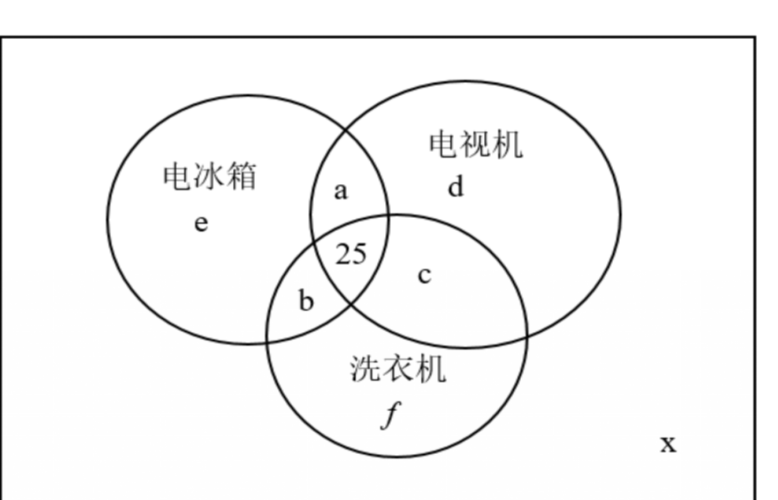
\includegraphics[width=0.42\textwidth]{figures/gao107_q15.png}
\end{center}

\step{所以 $25+a+b+e=45$①，$25+a+c+d=55$②,}
\step{$25+b+c+f=65$③,}
\step{把上面三个式子相加得 $2(a+b+c)+d+e+f=90$④,}
\step{对于拥有上述三种电器的任意两种的占 $35\%$，得 $a+b+c=35$⑤,}
\step{把⑤代入④可得到 $d+e+f=20$⑥,}
\step{因为农户共有 100 家，所以 $25+a+b+c+d+e+f+x=100$,}
\step{把⑤和⑥代入上式得 $x=20$，即一种电器也没有的农户所占比例为 $20\%$.}
\step{故选 $D$.}
\solend
\fi

\item 设 $d>0$，已知 $A,B$ 是两个数集. 若对任意 $x\in A$，都存在 $y\in B$，使得 $\lvert x-y\rvert<d$，则
称 $A$ 是 $B$ 的一个“$d-$邻集”. 现有下列两个命题：① $M=\{a+b\sqrt2\mid a,b\in\Z\}$ 是 $\Q$ 的一个
$\dfrac1{2025}$
一邻集；②若 $A$ 是 $B$ 的一个 $d-$邻集，则 $B$ 也是 $A$ 的一个 $d-$邻集；则\mbox{（\quad）}% 原卷把 d−邻集 的连字符断行后排成“一邻集”，照录

\keepwithprev
A. ①真②假\qquad B. ①假②真\qquad C. ①真②真\qquad D. ①假②假

\ifanswer
\solbegin
\step{对于①，任取 $M$ 中的元素 $x_0=a_0+b_0\sqrt2$,}
\step{则存在 $y_0\in\Q\cap\left(a_0+b_0\sqrt2-\dfrac1{2025},a_0+b_0\sqrt2+\dfrac1{2025}\right)$ 满足题意，故①正确；}
\step{对于②，取 $A=[-1,1]$,$B=[-2,2]$, $A$ 是 $B$ 的 $\dfrac12-$邻集，但反之不成立,}
\step{故②错误；}
\step{故选 $A$.}
\solend
\fi

\end{enumerate}

\bigsec{三、解答题}

\begin{enumerate}
\setcounter{enumi}{16}

\item 设 $a\in\R$，完成下列问题：

（1）求不等式 $3(a+1)x-3>2ax-3a$ 的解集 $M$；

（2）设集合 $A=\{x\mid x^2-ax+a^2-19=0\}$，$B=\{x\mid x^2-5x+6=0\}$，
$C=\{x\mid x^2+2x-8=0\}$. 若 $A\cap B\supset\varnothing$，$A\cap C=\varnothing$，求 $a$ 的值.

\ifanswer
\solbegin
\step{（1）不等式 $3(a+1)x-3>2ax-3a$ 可化为 $(a+3)x>3-3a$,}
\step{当 $a+3>0$，即 $a>-3$ 时，解得 $x>\dfrac{3-3a}{a+3}$,}
\step{当 $a+3=0$，即 $a=-3$ 时，不等式化为 $0\cdot x>12$，无解,}
\step{当 $a+3<0$，即 $a<-3$ 时，解得 $x<\dfrac{3-3a}{a+3}$,}
\step{综上所述，当 $a>-3$ 时，$M=\left(\dfrac{3-3a}{a+3},+\infty\right)$；}
\step{当 $a=-3$ 时，$M=\varnothing$；}
\step{当 $a<-3$ 时，$M=\left(-\infty,\dfrac{3-3a}{a+3}\right)$；}
\step{（2）$B=\{x\mid x^2-5x+6=0\}=\{2,3\}$，$C=\{x\mid x^2+2x-8=0\}=\{2,-4\}$,}
\step{因为 $A\cap B\supset\varnothing$，所以 $A\cap B\neq\varnothing$，又因为 $A\cap C=\varnothing$,}
\step{所以 $3\in A$，$2\notin A$，$-4\notin A$,}
\step{把 $x=3$ 代入方程 $x^2-ax+a^2-19=0$ 得 $9-3a+a^2-19=0$,}
\step{解得 $a=-2$ 或 $a=5$,}
\step{当 $a=-2$ 时，集合 $A=\{x\mid x^2+2x-15=0\}=\{3,-5\}$，符合题意,}
\step{当 $a=5$ 时，集合 $A=\{x\mid x^2-5x+6=0\}=\{3,2\}$，不符合题意，舍去,}
\step{综上所述，$a$ 的值为 $-2$.}
\solend
\fi

\item 完成下列问题：

（1）设 $x$、$y\in\R$，且 $x+y>5$，用反证法证明：$x>3$ 或 $y>2$；

（2）设 $x>0$，$a=x+1$，$b=\sqrt{x^2+7x+1}$，求 $\dfrac ba$ 的最大值.

\ifanswer
\solbegin
\step{（1）假设 $x\leqslant3$ 且 $y\leqslant2$，则 $x+y\leqslant3+2=5$，这与已知 $x+y>5$ 矛盾,}
\step{故 $x>3$ 或 $y>2$；}
\step{（2）$x>0$，$a=x+1$，$b=\sqrt{x^2+7x+1}$,}
\step{则 $\dfrac ba=\dfrac{\sqrt{x^2+7x+1}}{x+1}=\sqrt{\dfrac{x^2+7x+1}{x^2+2x+1}}=\sqrt{\dfrac{x^2+2x+1+5x}{x^2+2x+1}}$}
\step{$=\sqrt{1+\dfrac{5x}{x^2+2x+1}}=\sqrt{1+\dfrac{5}{x+\dfrac1x+2}}\leqslant\sqrt{1+\dfrac{5}{2\sqrt{x\cdot\dfrac1x}+2}}=\dfrac32$,}
\step{当且仅当 $x=\dfrac1x$，即 $x=1$ 时取等号，故 $\dfrac ba$ 的最大值为 $\dfrac32$.}
\solend
\fi

\item 已知函数 $f(x)=\lvert2x-a\rvert+a$.

（1）当 $a=2$ 时，求不等式 $f(x)\leqslant6+\lvert x+2\rvert$ 的解集；

（2）设 $g(x)=\lvert2x-1\rvert$，若不等式 $f(x)+g(x)\geqslant3$ 对一切 $x\in\R$ 恒成立，求实数 $a$ 的取值
范围.

\ifanswer
\solbegin
\ansspace*
\step{（1）$a=2$ 时，$f(x)=\lvert2x-2\rvert+2$,}
\step{则 $f(x)\leqslant6+\lvert x+2\rvert\Leftrightarrow\lvert2x-2\rvert+2\leqslant6+\lvert x+2\rvert$，即 $\lvert2x-2\rvert-\lvert x+2\rvert\leqslant4$,}
\step{当 $x<-2$ 时，$2-2x+x+2\leqslant4$，解得 $x\geqslant0$，与 $x<-2$ 取交集得 $\varnothing$,}
\step{当 $-2\leqslant x\leqslant1$ 时，$2-2x-x-2\leqslant4$，解得 $x\geqslant-\dfrac43$,}
\step{与 $-2\leqslant x\leqslant1$ 取交集得 $-\dfrac43\leqslant x\leqslant1$,}
\step{当 $x>1$ 时，$2x-2-x-2\leqslant4$，解得 $x\leqslant8$，与 $x>1$ 取交集得 $1<x\leqslant8$,}
\step{综上，不等式 $f(x)\leqslant6+\lvert x+2\rvert$ 的解集为 $\left\{x\,\middle|\,-\dfrac43\leqslant x\leqslant8\right\}$；}
\step{（2）$f(x)+g(x)\geqslant3$，即 $\lvert2x-a\rvert+a+\lvert2x-1\rvert\geqslant3$,}
\step{故 $\lvert2x-a\rvert+\lvert2x-1\rvert\geqslant3-a$,}
\step{当 $a\geqslant3$ 时，不等式显然成立,}
\step{当 $a<3$ 时,}
\step{由三角不等式得 $\lvert2x-a\rvert+\lvert2x-1\rvert\geqslant\lvert2x-a-(2x-1)\rvert=\lvert1-a\rvert$,}
\step{当且仅当 $(2x-a)(2x-1)\leqslant0$ 时取等号，因此 $\lvert1-a\rvert\geqslant3-a$,}
\step{平方得 $(1-a)^2\geqslant(3-a)^2$，解得 $a\geqslant2$，故 $2\leqslant a<3$.}
\step{综上，实数 $a$ 的取值范围是 $a\geqslant2$.}
\solend
\fi

\item 对于集合 $A,B$，定义集合 $A-B=\{x\mid x\in A$ 且 $x\notin B\}$.

（1）若 $A=\{1,2,3,4\}$,$B=\{3,4,5\}$，求集合 $A-B$ 和 $B-A$；

（2）给定集合 $A,B$，求所有满足方程组
\[
\begin{cases}
X\cap(A\cup B)=X\\
A\cap(B\cup X)=A\\
B\cap(A\cup X)=B\\
X\cap(A\cap B)=\varnothing
\end{cases}
\]
的集合 $X$（用 $A,B$ 表示）；

（3）用 $\lvert M\rvert$ 表示集合 $M$ 中的元素个数. 给定正整数 $n$，集合 $S=\{1,2,\cdots,n\}$. 对于实数
集的非空有限子集 $A,B$，定义集合 $C=\{x\mid x=a+b,a\in A,b\in B\}$. 求证：

$\lvert A-S\rvert+\lvert B-S\rvert+\lvert S-C\rvert\geqslant1$.

\ifanswer
\solbegin
\step{（1）由 $A=\{1,2,3,4\}$,$B=\{3,4,5\}$，则 $A-B=\{1,2\}$,$B-A=\{5\}$；}
\step{（2）由
$\begin{cases}
X\cap(A\cup B)=X\\
X\cap(A\cap B)=\varnothing
\end{cases}$，
得 $X\subseteq A-B$ 或 $X\subseteq B-A$,}
\step{再结合
$\begin{cases}
A\cap(B\cup X)=A\\
B\cap(A\cup X)=B
\end{cases}$，
得 $X=(A-B)\cup(B-A)$,}
\step{所以 $X=(A-B)\cup(B-A)$；}
\step{（3）$\lvert X\rvert$ 表示集合 $X$ 中的元素个数，则 $\lvert X\rvert\geqslant0$,}
\step{若 $A\cup B$ 中至少含有一个不在 $S$ 中的元素，则 $\lvert A-S\rvert+\lvert B-S\rvert\geqslant1$,}
\step{即 $\lvert A-S\rvert+\lvert B-S\rvert+\lvert S-C\rvert\geqslant1$.}
\step{若 $A\subseteq S$，且 $B\subseteq S$，则 $\lvert A-S\rvert=\lvert B-S\rvert=0$.}
\step{此时 $A$ 中最小的元素 $a\geqslant1$,$B$ 中最小的元素 $b\geqslant1$.}
\step{所以 $C$ 中最小的元素 $a+b\geqslant2$，则 $1\notin C$,}
\step{因为 $S=\{1,2,\cdots,n\}$，所以 $\lvert S-C\rvert\geqslant1$，即 $\lvert A-S\rvert+\lvert B-S\rvert+\lvert S-C\rvert\geqslant1$.}
\step{综上所述，$\lvert A-S\rvert+\lvert B-S\rvert+\lvert S-C\rvert\geqslant1$.}
\solend
\fi

\end{enumerate}

\end{document}
"
%
% 原始材料：微信公众号“魔都数学加油站”文章，作者破晓，2026-11-03 17:19 发布；
% 连载“27学年高一107”，原文标题“27学年高一107——2026-2027年上海市曹杨二中高一上10月月考”；
% 原文链接：https://mp.weixin.qq.com/s/IF4uB7aDNv-snYwbGMoDiQ。
% 正文为 10 张 PNG 页（第 1、2、4、6—9 页 4762×6735，第 3、5、10 页 2560×3620），题目下印有【解析】，为讲评版。
% 题目、解析均据原图转录；卷面水印及公众号页脚未录入。
% 第 11 题题干的三幅“出入相补”图（图 1—图 3）与第 15 题解析的三圆文氏图裁自原图、
% 去粉色水印转灰度（gao107_q11.png、gao107_q15.png），第 11 题图属题干（三版都出）、
% 第 15 题图属解析（仅答案版显示）。
%
% 卷首标题：原卷印作“2026-2027 年曹杨二中高一上 10 月月考”（公众号标题中的“上海市”
% 卷面标题行没有，本稿照卷面），年份区间按全稿惯例排 en dash；原卷未印副标题，本稿按题目内容
% 标为“集合与常用逻辑用语、不等式”。
%
% 与原卷的排版差异：
%   ① 原文从第 3 题起，填空题编号为 3—12、选择题为 13—16、解答题为 17—20，本稿保留原题号；
%   ② 原卷每题下直接印【解析】，本稿按全稿惯例将解析置于答案版；第 4 题只印【答案】另提 \ans{}；
%   ③ 原卷未印副标题，本稿按“知识模块”口径补出；
%   ④ 原卷填空横线按全稿惯例排为 \blankline[4.4em]；解答题按惯例加 \ansspace；选择题括号排
%      \mbox{（\quad）}、选项段前按惯例加 \keepwithprev；
%   ⑤ 原卷数集字母粗体与斜体混用（第 3 题 $\mathbf{R}$、第 4 题斜体 $R$、第 16 题粗体
%      $\mathbf{Z}$、$\mathbf{Q}$ 等），按全稿惯例统一改 \R、\Z、\Q。
%
% 原卷存疑：第 10 题解析“由 $\Delta=16m^2-8(2m^2+3m-2)\geqslant0$ 得 $m\leqslant\dfrac23$”
% 行末原卷无句读，照录。第 16 题解析②“取 $A=[-1,1]$，$B=[-2,2]$，$A$ 是 $B$ 的
% $\dfrac12$-邻集，但反之不成立”，据以判①真②假，照录。
%
% 行数核对：逐题数 \step/\stepm 条数，合计 112 条（Q3：5；Q4：0；Q5：2；Q6：2；Q7：2；
% Q8：4；Q9：8；Q10：4；Q11：9；Q12：3；Q13：5；Q14：3；Q15：12；Q16：5；Q17：15；
% Q18：6；Q19：15；Q20：12），与原卷印刷行逐题相等。第 4 题只印【答案】，提 \ans{}，
% 不计入 \step 账。
%
\documentclass[a4paper,11pt]{article}
\usepackage{common}

\begin{document}

\examtitlest[3]{2026--2027 年曹杨二中高一上 10 月月考}{集合与常用逻辑用语、不等式}

\bigsec{一、填空题}

\begin{enumerate}
\setcounter{enumi}{2}

\item 设 $a\in\R$，若 $3\in\{\sqrt3,a^2,a\}$，则 $a=$\blankline[4.4em].

\ifanswer
\solbegin
\step{因为 $3\in\{\sqrt3,a^2,a\}$，所以 $a^2=3$，解得 $a=\sqrt3$ 或 $a=-\sqrt3$,}
\step{当 $a=\sqrt3$ 时，集合为 $\{\sqrt3,3,\sqrt3\}$，不满足集合元素的互异性，舍去；}
\step{当 $a=-\sqrt3$ 时，集合为 $\{\sqrt3,3,-\sqrt3\}$，符合要求；}
\step{若 $a=3$，此时集合为 $\{\sqrt3,9,3\}$，符合要求；}
\step{综上，$a$ 为 $-\sqrt3$ 或 $3$.}
\solend
\fi

\item 设 $a\in\R$，已知集合 $A=\{x\mid x\leqslant a\}$，$B=\{x\mid x>2\}$. 若 $A\cup B=\R$，则 $a$ 的取值范围是\blankline[4.4em].

\ifanswer
\ans{$a\geqslant2$}
\fi

\item 设 $x>0$，$y>0$ 且 $x+3y=1$，则 $xy$ 的最大值为\blankline[4.4em].

\ifanswer
\solbegin
\step{由于 $x>0$，$y>0$ 且 $x+3y=1$，则 $1=x+3y\geqslant2\sqrt{3xy}$，得 $xy\leqslant\dfrac1{12}$,}
\step{当且仅当 $x=3y=\dfrac12$ 时取等号，则 $xy$ 的最大值为 $\dfrac1{12}$.}
\solend
\fi

\item 设 $a\in\R$，若集合$\left\{x\,\middle|\,\dfrac{ax}{x-1}=x\right\}$有且仅有两个子集，则 $a=$\blankline[4.4em].

\ifanswer
\solbegin
\step{由 $\dfrac{ax}{x-1}=x$ 得 $ax=x(x-1)$，即 $x(x-a-1)=0$,}
\step{所以此方程有两个相等的（不等于 1）的实数根或有一根为 1，所以 $a=-1$ 或 $0$.}
\solend
\fi

\item 已知全集 $U=\{x\mid x^2-8x-20<0\}$，集合 $A=\{x\mid 1-x^2>0$ 且 $x<0\}$，则 $\overline A=$\blankline[4.4em].

\ifanswer
\solbegin
\step{$U=\{x\mid-2<x<10\}$，$A=\{x\mid-1<x<0\}$,}
\step{所以 $\overline A=\{x\mid-2<x\leqslant-1$ 或 $0\leqslant x<10\}$.}
\solend
\fi

\item 设 $a,b\in\R$，若不等式 $-x^2-ax+b\geqslant0$ 的解集为 $[-2,3]$，则不等式 $\lvert ax+b\rvert<5$ 的解集为\blankline[4.4em].

\ifanswer
\solbegin
\step{由不等式 $-x^2-ax+b\geqslant0$ 的解集为 $[-2,3]$,}
\step{得 $-2$、$3$ 是方程 $-x^2-ax+b=0$ 的两个根，所以 $a=-1$，$b=6$.}
\step{解不等式 $\lvert-x+6\rvert<5$，得 $-5<x-6<5$，解得 $1<x<11$,}
\step{即所求不等式的解集为 $(1,11)$.}
\solend
\fi

\item 某货运卡车以 $x$ 千米／时的速度匀速行驶 300 千米，按交通法规限制 $50\leqslant x\leqslant100$，假设
柴油的价格为每升 6 元，汽车每小时耗油 $\left(4+\dfrac{x^2}{420}\right)$ 升，司机工资为每小时 46 元. 则当
$x=$\blankline[4.4em]（千米／时），这次行车的总费用（油费与司机工资的总和）最低.

\ifanswer
\solbegin
\step{因为卡车行驶 300 千米，速度为 $x$ 千米／时,}
\step{因此总用时为 $t=\dfrac{300}{x}$ 小时，其中 $50\leqslant x\leqslant100$,}
\step{每小时油费为 $6\cdot\left(4+\dfrac{x^2}{420}\right)$ 元，每小时司机工资为 46 元，因}
\step{此每小时总支出为 $6\cdot\left(4+\dfrac{x^2}{420}\right)+46=70+\dfrac{x^2}{70}$ 元.}
\step{设全程总费用为 $y$，则 $y=\dfrac{300}{x}\cdot\left(70+\dfrac{x^2}{70}\right)=\dfrac{21000}{x}+\dfrac{30x}{7}$,}
\step{因为 $50\leqslant x\leqslant100$，$\dfrac{21000}{x}+\dfrac{30x}{7}\geqslant2\sqrt{\dfrac{21000}{x}\cdot\dfrac{30x}{7}}=600$,}
\step{当且仅当 $\dfrac{21000}{x}=\dfrac{30x}{7}$，即 $x=70$ 时取等号，且 $70\in[50,100]$,}
\step{因此当 $x=70$ 千米／时，行车的总费用（油费与司机工资的总和）最低.}
\solend
\fi

\item 设 $x_1$、$x_2$ 是关于 $x$ 的方程 $2x^2-4mx+2m^2+3m-2=0$ 的两个实数根，则 $x_1^2+x_2^2$ 的最小值为\blankline[4.4em].

\ifanswer
\solbegin
\step{由题意得 $x_1+x_2=2m$，$x_1x_2=m^2+\dfrac{3m}{2}-1$,}
\step{由 $\Delta=16m^2-8(2m^2+3m-2)\geqslant0$ 得 $m\leqslant\dfrac23$}
\step{所以 $x_1^2+x_1^2=(x_1+x_2)^2-2x_1x_2=4m^2-2m^2+3m+2=2m^2-3m+2$,% 原卷左端作 x_1²+x_1²，照录
}
\step{结合二次函数的性质得，当 $m=\dfrac23$ 时取得最小值 $\dfrac89$.}
\solend
\fi

\item 小玲在钻研《九章算术》中“勾股容方”问题“今有勾五步，股十二步，问勾中容方几
何？”时，发现魏晋时期数学家刘徽在其《九章算术注》中利用出入相补原理给出了这个
问题的一般解法：如图 1，用对角线将长和宽分别为 $b$ 和 $a$ 的矩形分成两个直角三角形，
每个直角三角形再分成一个内接正方形（黄）和两个小直角三角形（朱、青）. 将三种颜色
的图形进行重组，得到如图 2 所示的矩形，该矩形长为 $a+b$，宽为内接正方形的边长
$d$. 由刘徽构造的图形可以得到许多重要的结论，如图 3，设 $D$ 为斜边 $BC$ 的中点，作直
角三角形 $ABC$ 的内接正方形对角线 $AE$，过点 $A$ 作 $AF\perp BC$ 于点 $F$，则下列四个推理中
正确的序号是\blankline[4.4em].

\begin{center}
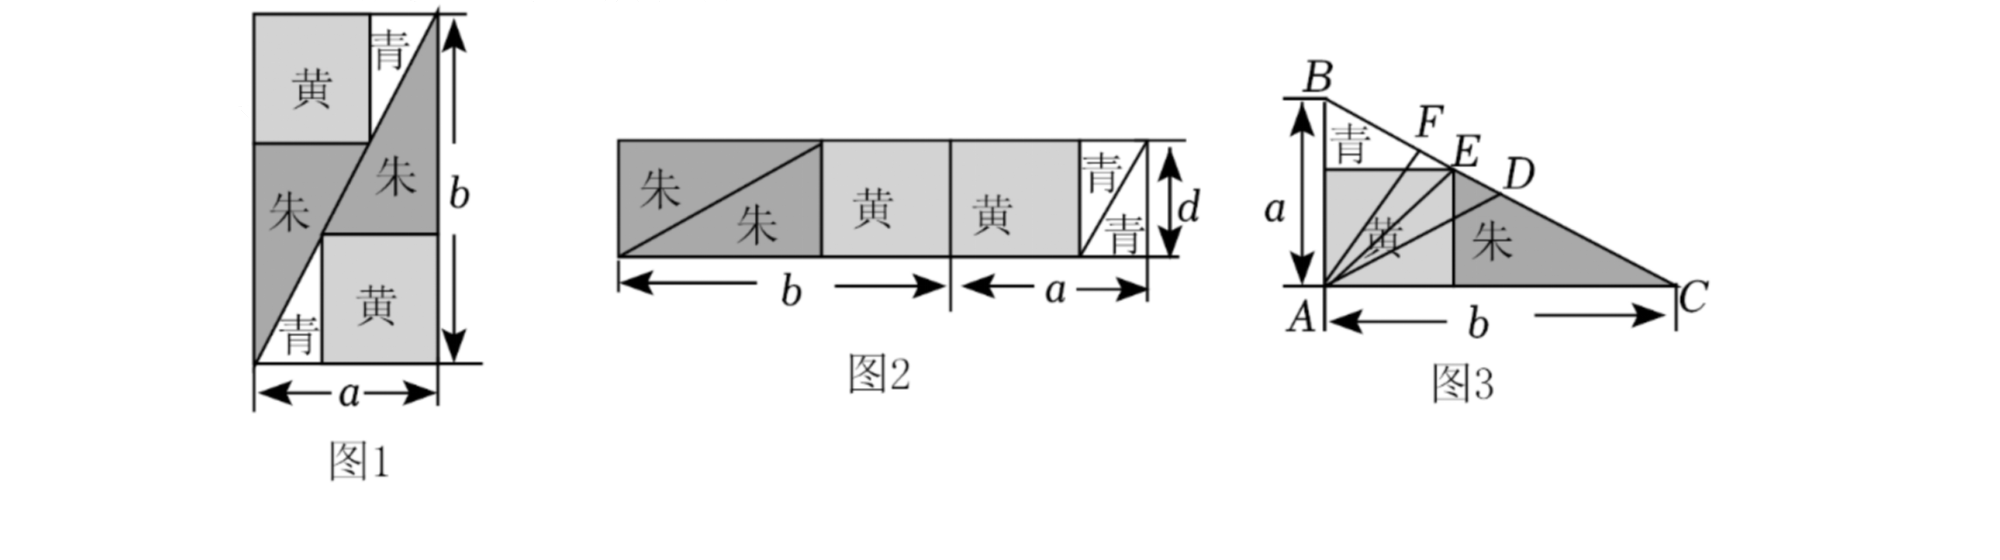
\includegraphics[width=0.86\textwidth]{figures/gao107_q11.png}
\end{center}

①由图 1 和图 2 面积相等得 $d=\dfrac{2ab}{a+b}$　　②由 $AE\geqslant AF$ 可得 $\sqrt{\dfrac{a^2+b^2}2}\geqslant\dfrac{a+b}2$

③由 $AD\geqslant AE$ 可得 $\sqrt{\dfrac{a^2+b^2}2}\geqslant\dfrac{2}{\dfrac1a+\dfrac1b}$　④由 $AD\geqslant AF$ 可得 $a^2+b^2\geqslant2ab$

\ifanswer
\solbegin
\step{对于①，由图 1 和图 2 面积相等得 $ab=(a+b)\times d$，所以 $d=\dfrac{ab}{a+b}$，故①错,}
\step{对于②，因为 $AF\perp BC$，所以 $\dfrac12ab=\dfrac12\sqrt{a^2+b^2}\times AF$,}
\step{所以 $AF=\dfrac{ab}{\sqrt{a^2+b^2}}$，$AE=\sqrt2d=\dfrac{\sqrt2ab}{a+b}$,}
\step{因为 $AE\geqslant AF$，所以 $\dfrac{\sqrt2ab}{a+b}\geqslant\dfrac{ab}{\sqrt{a^2+b^2}}$，整理得 $\sqrt{\dfrac{a^2+b^2}2}\geqslant\dfrac{a+b}2$，故②对,}
\step{对于③，因为 $D$ 是斜边 $BC$ 的中点，所以 $AD=\sqrt{\dfrac{a^2+b^2}2}$,}
\step{因为 $AD\geqslant AE$，所以 $\sqrt{\dfrac{a^2+b^2}2}\geqslant\dfrac{\sqrt2ab}{a+b}$，整理得 $\sqrt{\dfrac{a^2+b^2}2}\geqslant\dfrac{2}{\dfrac1a+\dfrac1b}$，故③对,}
\step{对于④，因为 $AD\geqslant AF$，所以 $\sqrt{\dfrac{a^2+b^2}2}\geqslant\dfrac{ab}{\sqrt{a^2+b^2}}$，整理得 $a^2+b^2\geqslant2ab$,}
\step{故④对,}
\step{故正确的是②③④.}
\solend
\fi

\item 设 $a,b,c,d\in\R$ 且$\lvert a-b\rvert\leqslant2$,$\lvert c-d\rvert\leqslant2$,$\lvert a\rvert\leqslant3$,$\lvert c\rvert\leqslant3$，则 $\lvert ad-bc\rvert$ 的最大值为\blankline[4.4em].% 原卷四处条件间均排半角逗号，照录

\ifanswer
\solbegin
\step{令 $a-b=e$,$c-d=f$，则 $\lvert e\rvert\leqslant2$,$\lvert f\rvert\leqslant2$,$\lvert a\rvert\leqslant3$,$\lvert c\rvert\leqslant3$}
\step{则 $\lvert ad-bc\rvert=\lvert a(c-f)-(a-e)c\rvert=\lvert ce-af\rvert\leqslant\lvert c\rvert\,\lvert e\rvert+\lvert a\rvert\,\lvert f\rvert\leqslant12$,}
\step{则 $\lvert ad-bc\rvert$ 的最大值为 12.}
\solend
\fi

\end{enumerate}

\bigsec{二、选择题}

\begin{enumerate}
\setcounter{enumi}{12}

\item 下列说法正确的是\mbox{（\quad）}

\keepwithprev
A. 若 $a>b>0$，则 $ac^2>bc^2$\qquad\qquad B. 若 $a<b<0$，则 $a^2>ab>b^2$

C. 若 $a>b$，则 $a^2>b^2$\qquad\qquad\qquad D. 若 $a<b$，则 $\dfrac1a>\dfrac1b$

\ifanswer
\solbegin
\step{$A$. 当 $a>b>0$ 时，取 $c=0$，则 $ac^2>bc^2$ 不成立，故 $A$ 错误；}
\step{$B$. 当 $a<b<0$ 时，由不等式的基本性质得 $a^2>ab>b^2>0$，故 $B$ 正确；}
\step{$C$. 当 $a>b$ 时，取 $a=0$，$b=-1$，则 $a^2>b^2$ 不成立，故 $C$ 错误；}
\step{$D$. 当 $a<b$ 时，取 $a=0$，$b=1$，则 $\dfrac1a>\dfrac1b$ 不成立，故 $D$ 错误.}
\step{故选 $B$.}
\solend
\fi

\item 小玲在学习《论语·子路》读到“其身正，不令而行；其身不正，虽令不从”，这句话的
数学含义可以理解为：“身正”是“令行”的\mbox{（\quad）}

\keepwithprev
A. 充分非必要条件\qquad\qquad B. 必要不充分条件

C. 充要条件\qquad\qquad\qquad D. 既非充分又非必要条件

\ifanswer
\solbegin
\step{其身正，不令而行，即身正$\Rightarrow$令行，所以“身正”是“令行”的充分条件；}
\step{又其身不正，虽令不从，即令行$\Rightarrow$身正，所以“身正”是“令行”的必要条件；}
\step{综上，“身正”是“令行”的充要条件. 故选 $C$.}
\solend
\fi

\item 某地对农户抽样调查，结果如下：电冰箱拥有率为 $45\%$，电视机拥有率为 $55\%$，洗衣
机拥有率为 $65\%$，拥有上述三种电器的任意两种的占 $35\%$，三种电器齐全的为 $25\%$，那
么一种电器也没有的农户所占比例是\mbox{（\quad）}

\keepwithprev
A. $12\%$\qquad B. $15\%$\qquad C. $18\%$\qquad D. $20\%$

\ifanswer
\solbegin
\step{设只有电冰箱和电视机的农户有 $a$ 家，只有电冰箱和洗衣机的农户有 $b$ 家,}
\step{只有洗衣机和电视机的农户有 $c$ 家,}
\step{只有电视机、电冰箱、洗衣机的分别有 $d$、$e$、$f$ 家,}
\step{没有任何电器的农户有 $x$ 家,}

\begin{center}
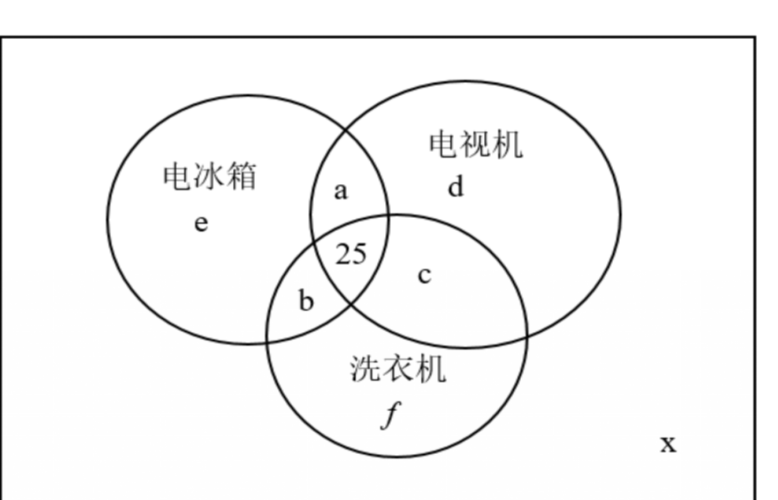
\includegraphics[width=0.42\textwidth]{figures/gao107_q15.png}
\end{center}

\step{所以 $25+a+b+e=45$①，$25+a+c+d=55$②,}
\step{$25+b+c+f=65$③,}
\step{把上面三个式子相加得 $2(a+b+c)+d+e+f=90$④,}
\step{对于拥有上述三种电器的任意两种的占 $35\%$，得 $a+b+c=35$⑤,}
\step{把⑤代入④可得到 $d+e+f=20$⑥,}
\step{因为农户共有 100 家，所以 $25+a+b+c+d+e+f+x=100$,}
\step{把⑤和⑥代入上式得 $x=20$，即一种电器也没有的农户所占比例为 $20\%$.}
\step{故选 $D$.}
\solend
\fi

\item 设 $d>0$，已知 $A,B$ 是两个数集. 若对任意 $x\in A$，都存在 $y\in B$，使得 $\lvert x-y\rvert<d$，则
称 $A$ 是 $B$ 的一个“$d-$邻集”. 现有下列两个命题：① $M=\{a+b\sqrt2\mid a,b\in\Z\}$ 是 $\Q$ 的一个
$\dfrac1{2025}$
一邻集；②若 $A$ 是 $B$ 的一个 $d-$邻集，则 $B$ 也是 $A$ 的一个 $d-$邻集；则\mbox{（\quad）}% 原卷把 d−邻集 的连字符断行后排成“一邻集”，照录

\keepwithprev
A. ①真②假\qquad B. ①假②真\qquad C. ①真②真\qquad D. ①假②假

\ifanswer
\solbegin
\step{对于①，任取 $M$ 中的元素 $x_0=a_0+b_0\sqrt2$,}
\step{则存在 $y_0\in\Q\cap\left(a_0+b_0\sqrt2-\dfrac1{2025},a_0+b_0\sqrt2+\dfrac1{2025}\right)$ 满足题意，故①正确；}
\step{对于②，取 $A=[-1,1]$,$B=[-2,2]$, $A$ 是 $B$ 的 $\dfrac12-$邻集，但反之不成立,}
\step{故②错误；}
\step{故选 $A$.}
\solend
\fi

\end{enumerate}

\bigsec{三、解答题}

\begin{enumerate}
\setcounter{enumi}{16}

\item 设 $a\in\R$，完成下列问题：

（1）求不等式 $3(a+1)x-3>2ax-3a$ 的解集 $M$；

（2）设集合 $A=\{x\mid x^2-ax+a^2-19=0\}$，$B=\{x\mid x^2-5x+6=0\}$，
$C=\{x\mid x^2+2x-8=0\}$. 若 $A\cap B\supset\varnothing$，$A\cap C=\varnothing$，求 $a$ 的值.

\ifanswer
\solbegin
\step{（1）不等式 $3(a+1)x-3>2ax-3a$ 可化为 $(a+3)x>3-3a$,}
\step{当 $a+3>0$，即 $a>-3$ 时，解得 $x>\dfrac{3-3a}{a+3}$,}
\step{当 $a+3=0$，即 $a=-3$ 时，不等式化为 $0\cdot x>12$，无解,}
\step{当 $a+3<0$，即 $a<-3$ 时，解得 $x<\dfrac{3-3a}{a+3}$,}
\step{综上所述，当 $a>-3$ 时，$M=\left(\dfrac{3-3a}{a+3},+\infty\right)$；}
\step{当 $a=-3$ 时，$M=\varnothing$；}
\step{当 $a<-3$ 时，$M=\left(-\infty,\dfrac{3-3a}{a+3}\right)$；}
\step{（2）$B=\{x\mid x^2-5x+6=0\}=\{2,3\}$，$C=\{x\mid x^2+2x-8=0\}=\{2,-4\}$,}
\step{因为 $A\cap B\supset\varnothing$，所以 $A\cap B\neq\varnothing$，又因为 $A\cap C=\varnothing$,}
\step{所以 $3\in A$，$2\notin A$，$-4\notin A$,}
\step{把 $x=3$ 代入方程 $x^2-ax+a^2-19=0$ 得 $9-3a+a^2-19=0$,}
\step{解得 $a=-2$ 或 $a=5$,}
\step{当 $a=-2$ 时，集合 $A=\{x\mid x^2+2x-15=0\}=\{3,-5\}$，符合题意,}
\step{当 $a=5$ 时，集合 $A=\{x\mid x^2-5x+6=0\}=\{3,2\}$，不符合题意，舍去,}
\step{综上所述，$a$ 的值为 $-2$.}
\solend
\fi

\item 完成下列问题：

（1）设 $x$、$y\in\R$，且 $x+y>5$，用反证法证明：$x>3$ 或 $y>2$；

（2）设 $x>0$，$a=x+1$，$b=\sqrt{x^2+7x+1}$，求 $\dfrac ba$ 的最大值.

\ifanswer
\solbegin
\step{（1）假设 $x\leqslant3$ 且 $y\leqslant2$，则 $x+y\leqslant3+2=5$，这与已知 $x+y>5$ 矛盾,}
\step{故 $x>3$ 或 $y>2$；}
\step{（2）$x>0$，$a=x+1$，$b=\sqrt{x^2+7x+1}$,}
\step{则 $\dfrac ba=\dfrac{\sqrt{x^2+7x+1}}{x+1}=\sqrt{\dfrac{x^2+7x+1}{x^2+2x+1}}=\sqrt{\dfrac{x^2+2x+1+5x}{x^2+2x+1}}$}
\step{$=\sqrt{1+\dfrac{5x}{x^2+2x+1}}=\sqrt{1+\dfrac{5}{x+\dfrac1x+2}}\leqslant\sqrt{1+\dfrac{5}{2\sqrt{x\cdot\dfrac1x}+2}}=\dfrac32$,}
\step{当且仅当 $x=\dfrac1x$，即 $x=1$ 时取等号，故 $\dfrac ba$ 的最大值为 $\dfrac32$.}
\solend
\fi

\item 已知函数 $f(x)=\lvert2x-a\rvert+a$.

（1）当 $a=2$ 时，求不等式 $f(x)\leqslant6+\lvert x+2\rvert$ 的解集；

（2）设 $g(x)=\lvert2x-1\rvert$，若不等式 $f(x)+g(x)\geqslant3$ 对一切 $x\in\R$ 恒成立，求实数 $a$ 的取值
范围.

\ifanswer
\solbegin
\ansspace*
\step{（1）$a=2$ 时，$f(x)=\lvert2x-2\rvert+2$,}
\step{则 $f(x)\leqslant6+\lvert x+2\rvert\Leftrightarrow\lvert2x-2\rvert+2\leqslant6+\lvert x+2\rvert$，即 $\lvert2x-2\rvert-\lvert x+2\rvert\leqslant4$,}
\step{当 $x<-2$ 时，$2-2x+x+2\leqslant4$，解得 $x\geqslant0$，与 $x<-2$ 取交集得 $\varnothing$,}
\step{当 $-2\leqslant x\leqslant1$ 时，$2-2x-x-2\leqslant4$，解得 $x\geqslant-\dfrac43$,}
\step{与 $-2\leqslant x\leqslant1$ 取交集得 $-\dfrac43\leqslant x\leqslant1$,}
\step{当 $x>1$ 时，$2x-2-x-2\leqslant4$，解得 $x\leqslant8$，与 $x>1$ 取交集得 $1<x\leqslant8$,}
\step{综上，不等式 $f(x)\leqslant6+\lvert x+2\rvert$ 的解集为 $\left\{x\,\middle|\,-\dfrac43\leqslant x\leqslant8\right\}$；}
\step{（2）$f(x)+g(x)\geqslant3$，即 $\lvert2x-a\rvert+a+\lvert2x-1\rvert\geqslant3$,}
\step{故 $\lvert2x-a\rvert+\lvert2x-1\rvert\geqslant3-a$,}
\step{当 $a\geqslant3$ 时，不等式显然成立,}
\step{当 $a<3$ 时,}
\step{由三角不等式得 $\lvert2x-a\rvert+\lvert2x-1\rvert\geqslant\lvert2x-a-(2x-1)\rvert=\lvert1-a\rvert$,}
\step{当且仅当 $(2x-a)(2x-1)\leqslant0$ 时取等号，因此 $\lvert1-a\rvert\geqslant3-a$,}
\step{平方得 $(1-a)^2\geqslant(3-a)^2$，解得 $a\geqslant2$，故 $2\leqslant a<3$.}
\step{综上，实数 $a$ 的取值范围是 $a\geqslant2$.}
\solend
\fi

\item 对于集合 $A,B$，定义集合 $A-B=\{x\mid x\in A$ 且 $x\notin B\}$.

（1）若 $A=\{1,2,3,4\}$,$B=\{3,4,5\}$，求集合 $A-B$ 和 $B-A$；

（2）给定集合 $A,B$，求所有满足方程组
\[
\begin{cases}
X\cap(A\cup B)=X\\
A\cap(B\cup X)=A\\
B\cap(A\cup X)=B\\
X\cap(A\cap B)=\varnothing
\end{cases}
\]
的集合 $X$（用 $A,B$ 表示）；

（3）用 $\lvert M\rvert$ 表示集合 $M$ 中的元素个数. 给定正整数 $n$，集合 $S=\{1,2,\cdots,n\}$. 对于实数
集的非空有限子集 $A,B$，定义集合 $C=\{x\mid x=a+b,a\in A,b\in B\}$. 求证：

$\lvert A-S\rvert+\lvert B-S\rvert+\lvert S-C\rvert\geqslant1$.

\ifanswer
\solbegin
\step{（1）由 $A=\{1,2,3,4\}$,$B=\{3,4,5\}$，则 $A-B=\{1,2\}$,$B-A=\{5\}$；}
\step{（2）由
$\begin{cases}
X\cap(A\cup B)=X\\
X\cap(A\cap B)=\varnothing
\end{cases}$，
得 $X\subseteq A-B$ 或 $X\subseteq B-A$,}
\step{再结合
$\begin{cases}
A\cap(B\cup X)=A\\
B\cap(A\cup X)=B
\end{cases}$，
得 $X=(A-B)\cup(B-A)$,}
\step{所以 $X=(A-B)\cup(B-A)$；}
\step{（3）$\lvert X\rvert$ 表示集合 $X$ 中的元素个数，则 $\lvert X\rvert\geqslant0$,}
\step{若 $A\cup B$ 中至少含有一个不在 $S$ 中的元素，则 $\lvert A-S\rvert+\lvert B-S\rvert\geqslant1$,}
\step{即 $\lvert A-S\rvert+\lvert B-S\rvert+\lvert S-C\rvert\geqslant1$.}
\step{若 $A\subseteq S$，且 $B\subseteq S$，则 $\lvert A-S\rvert=\lvert B-S\rvert=0$.}
\step{此时 $A$ 中最小的元素 $a\geqslant1$,$B$ 中最小的元素 $b\geqslant1$.}
\step{所以 $C$ 中最小的元素 $a+b\geqslant2$，则 $1\notin C$,}
\step{因为 $S=\{1,2,\cdots,n\}$，所以 $\lvert S-C\rvert\geqslant1$，即 $\lvert A-S\rvert+\lvert B-S\rvert+\lvert S-C\rvert\geqslant1$.}
\step{综上所述，$\lvert A-S\rvert+\lvert B-S\rvert+\lvert S-C\rvert\geqslant1$.}
\solend
\fi

\end{enumerate}

\end{document}
"
%
% 原始材料：微信公众号“魔都数学加油站”文章，作者破晓，2026-11-03 17:19 发布；
% 连载“27学年高一107”，原文标题“27学年高一107——2026-2027年上海市曹杨二中高一上10月月考”；
% 原文链接：https://mp.weixin.qq.com/s/IF4uB7aDNv-snYwbGMoDiQ。
% 正文为 10 张 PNG 页（第 1、2、4、6—9 页 4762×6735，第 3、5、10 页 2560×3620），题目下印有【解析】，为讲评版。
% 题目、解析均据原图转录；卷面水印及公众号页脚未录入。
% 第 11 题题干的三幅“出入相补”图（图 1—图 3）与第 15 题解析的三圆文氏图裁自原图、
% 去粉色水印转灰度（gao107_q11.png、gao107_q15.png），第 11 题图属题干（三版都出）、
% 第 15 题图属解析（仅答案版显示）。
%
% 卷首标题：原卷印作“2026-2027 年曹杨二中高一上 10 月月考”（公众号标题中的“上海市”
% 卷面标题行没有，本稿照卷面），年份区间按全稿惯例排 en dash；原卷未印副标题，本稿按题目内容
% 标为“集合与常用逻辑用语、不等式”。
%
% 与原卷的排版差异：
%   ① 原文从第 3 题起，填空题编号为 3—12、选择题为 13—16、解答题为 17—20，本稿保留原题号；
%   ② 原卷每题下直接印【解析】，本稿按全稿惯例将解析置于答案版；第 4 题只印【答案】另提 \ans{}；
%   ③ 原卷未印副标题，本稿按“知识模块”口径补出；
%   ④ 原卷填空横线按全稿惯例排为 \blankline[4.4em]；解答题按惯例加 \ansspace；选择题括号排
%      \mbox{（\quad）}、选项段前按惯例加 \keepwithprev；
%   ⑤ 原卷数集字母粗体与斜体混用（第 3 题 $\mathbf{R}$、第 4 题斜体 $R$、第 16 题粗体
%      $\mathbf{Z}$、$\mathbf{Q}$ 等），按全稿惯例统一改 \R、\Z、\Q。
%
% 原卷存疑：第 10 题解析“由 $\Delta=16m^2-8(2m^2+3m-2)\geqslant0$ 得 $m\leqslant\dfrac23$”
% 行末原卷无句读，照录。第 16 题解析②“取 $A=[-1,1]$，$B=[-2,2]$，$A$ 是 $B$ 的
% $\dfrac12$-邻集，但反之不成立”，据以判①真②假，照录。
%
% 行数核对：逐题数 \step/\stepm 条数，合计 112 条（Q3：5；Q4：0；Q5：2；Q6：2；Q7：2；
% Q8：4；Q9：8；Q10：4；Q11：9；Q12：3；Q13：5；Q14：3；Q15：12；Q16：5；Q17：15；
% Q18：6；Q19：15；Q20：12），与原卷印刷行逐题相等。第 4 题只印【答案】，提 \ans{}，
% 不计入 \step 账。
%
\documentclass[a4paper,11pt]{article}
\usepackage{common}

\begin{document}

\examtitlest[3]{2026--2027 年曹杨二中高一上 10 月月考}{集合与常用逻辑用语、不等式}

\bigsec{一、填空题}

\begin{enumerate}
\setcounter{enumi}{2}

\item 设 $a\in\R$，若 $3\in\{\sqrt3,a^2,a\}$，则 $a=$\blankline[4.4em].

\ifanswer
\solbegin
\step{因为 $3\in\{\sqrt3,a^2,a\}$，所以 $a^2=3$，解得 $a=\sqrt3$ 或 $a=-\sqrt3$,}
\step{当 $a=\sqrt3$ 时，集合为 $\{\sqrt3,3,\sqrt3\}$，不满足集合元素的互异性，舍去；}
\step{当 $a=-\sqrt3$ 时，集合为 $\{\sqrt3,3,-\sqrt3\}$，符合要求；}
\step{若 $a=3$，此时集合为 $\{\sqrt3,9,3\}$，符合要求；}
\step{综上，$a$ 为 $-\sqrt3$ 或 $3$.}
\solend
\fi

\item 设 $a\in\R$，已知集合 $A=\{x\mid x\leqslant a\}$，$B=\{x\mid x>2\}$. 若 $A\cup B=\R$，则 $a$ 的取值范围是\blankline[4.4em].

\ifanswer
\ans{$a\geqslant2$}
\fi

\item 设 $x>0$，$y>0$ 且 $x+3y=1$，则 $xy$ 的最大值为\blankline[4.4em].

\ifanswer
\solbegin
\step{由于 $x>0$，$y>0$ 且 $x+3y=1$，则 $1=x+3y\geqslant2\sqrt{3xy}$，得 $xy\leqslant\dfrac1{12}$,}
\step{当且仅当 $x=3y=\dfrac12$ 时取等号，则 $xy$ 的最大值为 $\dfrac1{12}$.}
\solend
\fi

\item 设 $a\in\R$，若集合$\left\{x\,\middle|\,\dfrac{ax}{x-1}=x\right\}$有且仅有两个子集，则 $a=$\blankline[4.4em].

\ifanswer
\solbegin
\step{由 $\dfrac{ax}{x-1}=x$ 得 $ax=x(x-1)$，即 $x(x-a-1)=0$,}
\step{所以此方程有两个相等的（不等于 1）的实数根或有一根为 1，所以 $a=-1$ 或 $0$.}
\solend
\fi

\item 已知全集 $U=\{x\mid x^2-8x-20<0\}$，集合 $A=\{x\mid 1-x^2>0$ 且 $x<0\}$，则 $\overline A=$\blankline[4.4em].

\ifanswer
\solbegin
\step{$U=\{x\mid-2<x<10\}$，$A=\{x\mid-1<x<0\}$,}
\step{所以 $\overline A=\{x\mid-2<x\leqslant-1$ 或 $0\leqslant x<10\}$.}
\solend
\fi

\item 设 $a,b\in\R$，若不等式 $-x^2-ax+b\geqslant0$ 的解集为 $[-2,3]$，则不等式 $\lvert ax+b\rvert<5$ 的解集为\blankline[4.4em].

\ifanswer
\solbegin
\step{由不等式 $-x^2-ax+b\geqslant0$ 的解集为 $[-2,3]$,}
\step{得 $-2$、$3$ 是方程 $-x^2-ax+b=0$ 的两个根，所以 $a=-1$，$b=6$.}
\step{解不等式 $\lvert-x+6\rvert<5$，得 $-5<x-6<5$，解得 $1<x<11$,}
\step{即所求不等式的解集为 $(1,11)$.}
\solend
\fi

\item 某货运卡车以 $x$ 千米／时的速度匀速行驶 300 千米，按交通法规限制 $50\leqslant x\leqslant100$，假设
柴油的价格为每升 6 元，汽车每小时耗油 $\left(4+\dfrac{x^2}{420}\right)$ 升，司机工资为每小时 46 元. 则当
$x=$\blankline[4.4em]（千米／时），这次行车的总费用（油费与司机工资的总和）最低.

\ifanswer
\solbegin
\step{因为卡车行驶 300 千米，速度为 $x$ 千米／时,}
\step{因此总用时为 $t=\dfrac{300}{x}$ 小时，其中 $50\leqslant x\leqslant100$,}
\step{每小时油费为 $6\cdot\left(4+\dfrac{x^2}{420}\right)$ 元，每小时司机工资为 46 元，因}
\step{此每小时总支出为 $6\cdot\left(4+\dfrac{x^2}{420}\right)+46=70+\dfrac{x^2}{70}$ 元.}
\step{设全程总费用为 $y$，则 $y=\dfrac{300}{x}\cdot\left(70+\dfrac{x^2}{70}\right)=\dfrac{21000}{x}+\dfrac{30x}{7}$,}
\step{因为 $50\leqslant x\leqslant100$，$\dfrac{21000}{x}+\dfrac{30x}{7}\geqslant2\sqrt{\dfrac{21000}{x}\cdot\dfrac{30x}{7}}=600$,}
\step{当且仅当 $\dfrac{21000}{x}=\dfrac{30x}{7}$，即 $x=70$ 时取等号，且 $70\in[50,100]$,}
\step{因此当 $x=70$ 千米／时，行车的总费用（油费与司机工资的总和）最低.}
\solend
\fi

\item 设 $x_1$、$x_2$ 是关于 $x$ 的方程 $2x^2-4mx+2m^2+3m-2=0$ 的两个实数根，则 $x_1^2+x_2^2$ 的最小值为\blankline[4.4em].

\ifanswer
\solbegin
\step{由题意得 $x_1+x_2=2m$，$x_1x_2=m^2+\dfrac{3m}{2}-1$,}
\step{由 $\Delta=16m^2-8(2m^2+3m-2)\geqslant0$ 得 $m\leqslant\dfrac23$}
\step{所以 $x_1^2+x_1^2=(x_1+x_2)^2-2x_1x_2=4m^2-2m^2+3m+2=2m^2-3m+2$,% 原卷左端作 x_1²+x_1²，照录
}
\step{结合二次函数的性质得，当 $m=\dfrac23$ 时取得最小值 $\dfrac89$.}
\solend
\fi

\item 小玲在钻研《九章算术》中“勾股容方”问题“今有勾五步，股十二步，问勾中容方几
何？”时，发现魏晋时期数学家刘徽在其《九章算术注》中利用出入相补原理给出了这个
问题的一般解法：如图 1，用对角线将长和宽分别为 $b$ 和 $a$ 的矩形分成两个直角三角形，
每个直角三角形再分成一个内接正方形（黄）和两个小直角三角形（朱、青）. 将三种颜色
的图形进行重组，得到如图 2 所示的矩形，该矩形长为 $a+b$，宽为内接正方形的边长
$d$. 由刘徽构造的图形可以得到许多重要的结论，如图 3，设 $D$ 为斜边 $BC$ 的中点，作直
角三角形 $ABC$ 的内接正方形对角线 $AE$，过点 $A$ 作 $AF\perp BC$ 于点 $F$，则下列四个推理中
正确的序号是\blankline[4.4em].

\begin{center}
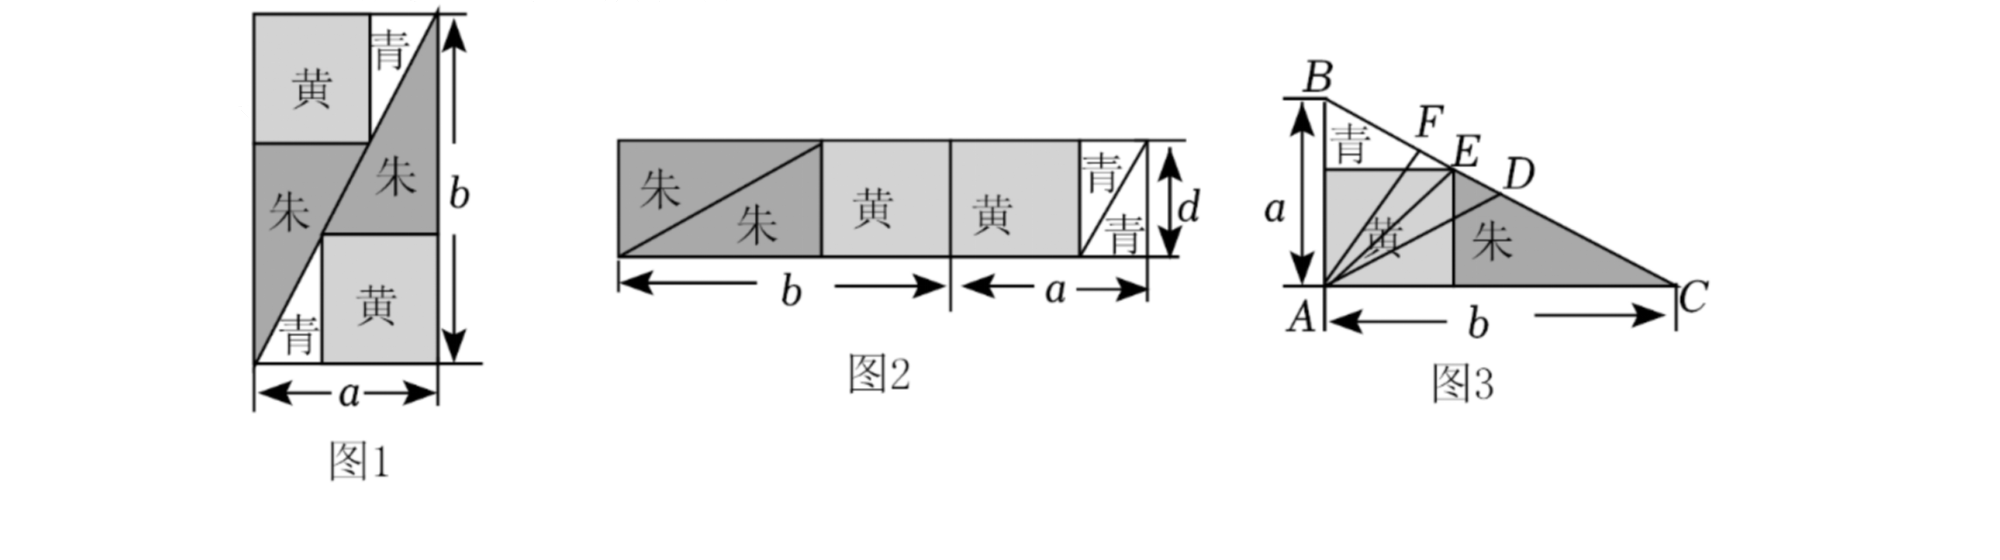
\includegraphics[width=0.86\textwidth]{figures/gao107_q11.png}
\end{center}

①由图 1 和图 2 面积相等得 $d=\dfrac{2ab}{a+b}$　　②由 $AE\geqslant AF$ 可得 $\sqrt{\dfrac{a^2+b^2}2}\geqslant\dfrac{a+b}2$

③由 $AD\geqslant AE$ 可得 $\sqrt{\dfrac{a^2+b^2}2}\geqslant\dfrac{2}{\dfrac1a+\dfrac1b}$　④由 $AD\geqslant AF$ 可得 $a^2+b^2\geqslant2ab$

\ifanswer
\solbegin
\step{对于①，由图 1 和图 2 面积相等得 $ab=(a+b)\times d$，所以 $d=\dfrac{ab}{a+b}$，故①错,}
\step{对于②，因为 $AF\perp BC$，所以 $\dfrac12ab=\dfrac12\sqrt{a^2+b^2}\times AF$,}
\step{所以 $AF=\dfrac{ab}{\sqrt{a^2+b^2}}$，$AE=\sqrt2d=\dfrac{\sqrt2ab}{a+b}$,}
\step{因为 $AE\geqslant AF$，所以 $\dfrac{\sqrt2ab}{a+b}\geqslant\dfrac{ab}{\sqrt{a^2+b^2}}$，整理得 $\sqrt{\dfrac{a^2+b^2}2}\geqslant\dfrac{a+b}2$，故②对,}
\step{对于③，因为 $D$ 是斜边 $BC$ 的中点，所以 $AD=\sqrt{\dfrac{a^2+b^2}2}$,}
\step{因为 $AD\geqslant AE$，所以 $\sqrt{\dfrac{a^2+b^2}2}\geqslant\dfrac{\sqrt2ab}{a+b}$，整理得 $\sqrt{\dfrac{a^2+b^2}2}\geqslant\dfrac{2}{\dfrac1a+\dfrac1b}$，故③对,}
\step{对于④，因为 $AD\geqslant AF$，所以 $\sqrt{\dfrac{a^2+b^2}2}\geqslant\dfrac{ab}{\sqrt{a^2+b^2}}$，整理得 $a^2+b^2\geqslant2ab$,}
\step{故④对,}
\step{故正确的是②③④.}
\solend
\fi

\item 设 $a,b,c,d\in\R$ 且$\lvert a-b\rvert\leqslant2$,$\lvert c-d\rvert\leqslant2$,$\lvert a\rvert\leqslant3$,$\lvert c\rvert\leqslant3$，则 $\lvert ad-bc\rvert$ 的最大值为\blankline[4.4em].% 原卷四处条件间均排半角逗号，照录

\ifanswer
\solbegin
\step{令 $a-b=e$,$c-d=f$，则 $\lvert e\rvert\leqslant2$,$\lvert f\rvert\leqslant2$,$\lvert a\rvert\leqslant3$,$\lvert c\rvert\leqslant3$}
\step{则 $\lvert ad-bc\rvert=\lvert a(c-f)-(a-e)c\rvert=\lvert ce-af\rvert\leqslant\lvert c\rvert\,\lvert e\rvert+\lvert a\rvert\,\lvert f\rvert\leqslant12$,}
\step{则 $\lvert ad-bc\rvert$ 的最大值为 12.}
\solend
\fi

\end{enumerate}

\bigsec{二、选择题}

\begin{enumerate}
\setcounter{enumi}{12}

\item 下列说法正确的是\mbox{（\quad）}

\keepwithprev
A. 若 $a>b>0$，则 $ac^2>bc^2$\qquad\qquad B. 若 $a<b<0$，则 $a^2>ab>b^2$

C. 若 $a>b$，则 $a^2>b^2$\qquad\qquad\qquad D. 若 $a<b$，则 $\dfrac1a>\dfrac1b$

\ifanswer
\solbegin
\step{$A$. 当 $a>b>0$ 时，取 $c=0$，则 $ac^2>bc^2$ 不成立，故 $A$ 错误；}
\step{$B$. 当 $a<b<0$ 时，由不等式的基本性质得 $a^2>ab>b^2>0$，故 $B$ 正确；}
\step{$C$. 当 $a>b$ 时，取 $a=0$，$b=-1$，则 $a^2>b^2$ 不成立，故 $C$ 错误；}
\step{$D$. 当 $a<b$ 时，取 $a=0$，$b=1$，则 $\dfrac1a>\dfrac1b$ 不成立，故 $D$ 错误.}
\step{故选 $B$.}
\solend
\fi

\item 小玲在学习《论语·子路》读到“其身正，不令而行；其身不正，虽令不从”，这句话的
数学含义可以理解为：“身正”是“令行”的\mbox{（\quad）}

\keepwithprev
A. 充分非必要条件\qquad\qquad B. 必要不充分条件

C. 充要条件\qquad\qquad\qquad D. 既非充分又非必要条件

\ifanswer
\solbegin
\step{其身正，不令而行，即身正$\Rightarrow$令行，所以“身正”是“令行”的充分条件；}
\step{又其身不正，虽令不从，即令行$\Rightarrow$身正，所以“身正”是“令行”的必要条件；}
\step{综上，“身正”是“令行”的充要条件. 故选 $C$.}
\solend
\fi

\item 某地对农户抽样调查，结果如下：电冰箱拥有率为 $45\%$，电视机拥有率为 $55\%$，洗衣
机拥有率为 $65\%$，拥有上述三种电器的任意两种的占 $35\%$，三种电器齐全的为 $25\%$，那
么一种电器也没有的农户所占比例是\mbox{（\quad）}

\keepwithprev
A. $12\%$\qquad B. $15\%$\qquad C. $18\%$\qquad D. $20\%$

\ifanswer
\solbegin
\step{设只有电冰箱和电视机的农户有 $a$ 家，只有电冰箱和洗衣机的农户有 $b$ 家,}
\step{只有洗衣机和电视机的农户有 $c$ 家,}
\step{只有电视机、电冰箱、洗衣机的分别有 $d$、$e$、$f$ 家,}
\step{没有任何电器的农户有 $x$ 家,}

\begin{center}
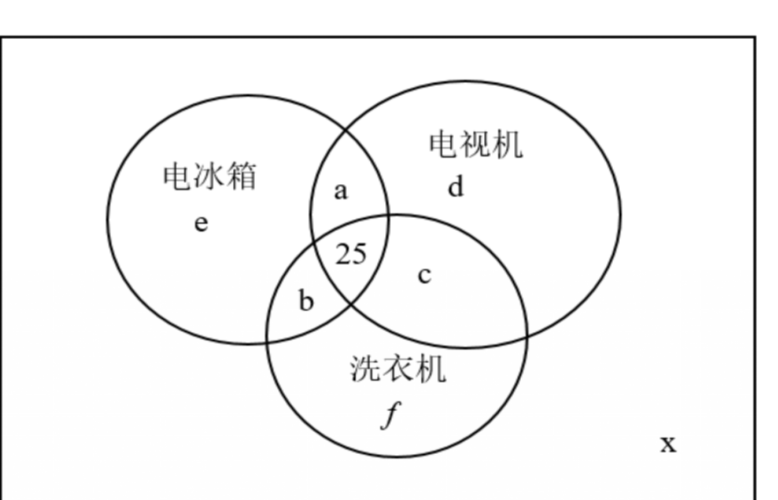
\includegraphics[width=0.42\textwidth]{figures/gao107_q15.png}
\end{center}

\step{所以 $25+a+b+e=45$①，$25+a+c+d=55$②,}
\step{$25+b+c+f=65$③,}
\step{把上面三个式子相加得 $2(a+b+c)+d+e+f=90$④,}
\step{对于拥有上述三种电器的任意两种的占 $35\%$，得 $a+b+c=35$⑤,}
\step{把⑤代入④可得到 $d+e+f=20$⑥,}
\step{因为农户共有 100 家，所以 $25+a+b+c+d+e+f+x=100$,}
\step{把⑤和⑥代入上式得 $x=20$，即一种电器也没有的农户所占比例为 $20\%$.}
\step{故选 $D$.}
\solend
\fi

\item 设 $d>0$，已知 $A,B$ 是两个数集. 若对任意 $x\in A$，都存在 $y\in B$，使得 $\lvert x-y\rvert<d$，则
称 $A$ 是 $B$ 的一个“$d-$邻集”. 现有下列两个命题：① $M=\{a+b\sqrt2\mid a,b\in\Z\}$ 是 $\Q$ 的一个
$\dfrac1{2025}$
一邻集；②若 $A$ 是 $B$ 的一个 $d-$邻集，则 $B$ 也是 $A$ 的一个 $d-$邻集；则\mbox{（\quad）}% 原卷把 d−邻集 的连字符断行后排成“一邻集”，照录

\keepwithprev
A. ①真②假\qquad B. ①假②真\qquad C. ①真②真\qquad D. ①假②假

\ifanswer
\solbegin
\step{对于①，任取 $M$ 中的元素 $x_0=a_0+b_0\sqrt2$,}
\step{则存在 $y_0\in\Q\cap\left(a_0+b_0\sqrt2-\dfrac1{2025},a_0+b_0\sqrt2+\dfrac1{2025}\right)$ 满足题意，故①正确；}
\step{对于②，取 $A=[-1,1]$,$B=[-2,2]$, $A$ 是 $B$ 的 $\dfrac12-$邻集，但反之不成立,}
\step{故②错误；}
\step{故选 $A$.}
\solend
\fi

\end{enumerate}

\bigsec{三、解答题}

\begin{enumerate}
\setcounter{enumi}{16}

\item 设 $a\in\R$，完成下列问题：

（1）求不等式 $3(a+1)x-3>2ax-3a$ 的解集 $M$；

（2）设集合 $A=\{x\mid x^2-ax+a^2-19=0\}$，$B=\{x\mid x^2-5x+6=0\}$，
$C=\{x\mid x^2+2x-8=0\}$. 若 $A\cap B\supset\varnothing$，$A\cap C=\varnothing$，求 $a$ 的值.

\ifanswer
\solbegin
\step{（1）不等式 $3(a+1)x-3>2ax-3a$ 可化为 $(a+3)x>3-3a$,}
\step{当 $a+3>0$，即 $a>-3$ 时，解得 $x>\dfrac{3-3a}{a+3}$,}
\step{当 $a+3=0$，即 $a=-3$ 时，不等式化为 $0\cdot x>12$，无解,}
\step{当 $a+3<0$，即 $a<-3$ 时，解得 $x<\dfrac{3-3a}{a+3}$,}
\step{综上所述，当 $a>-3$ 时，$M=\left(\dfrac{3-3a}{a+3},+\infty\right)$；}
\step{当 $a=-3$ 时，$M=\varnothing$；}
\step{当 $a<-3$ 时，$M=\left(-\infty,\dfrac{3-3a}{a+3}\right)$；}
\step{（2）$B=\{x\mid x^2-5x+6=0\}=\{2,3\}$，$C=\{x\mid x^2+2x-8=0\}=\{2,-4\}$,}
\step{因为 $A\cap B\supset\varnothing$，所以 $A\cap B\neq\varnothing$，又因为 $A\cap C=\varnothing$,}
\step{所以 $3\in A$，$2\notin A$，$-4\notin A$,}
\step{把 $x=3$ 代入方程 $x^2-ax+a^2-19=0$ 得 $9-3a+a^2-19=0$,}
\step{解得 $a=-2$ 或 $a=5$,}
\step{当 $a=-2$ 时，集合 $A=\{x\mid x^2+2x-15=0\}=\{3,-5\}$，符合题意,}
\step{当 $a=5$ 时，集合 $A=\{x\mid x^2-5x+6=0\}=\{3,2\}$，不符合题意，舍去,}
\step{综上所述，$a$ 的值为 $-2$.}
\solend
\fi

\item 完成下列问题：

（1）设 $x$、$y\in\R$，且 $x+y>5$，用反证法证明：$x>3$ 或 $y>2$；

（2）设 $x>0$，$a=x+1$，$b=\sqrt{x^2+7x+1}$，求 $\dfrac ba$ 的最大值.

\ifanswer
\solbegin
\step{（1）假设 $x\leqslant3$ 且 $y\leqslant2$，则 $x+y\leqslant3+2=5$，这与已知 $x+y>5$ 矛盾,}
\step{故 $x>3$ 或 $y>2$；}
\step{（2）$x>0$，$a=x+1$，$b=\sqrt{x^2+7x+1}$,}
\step{则 $\dfrac ba=\dfrac{\sqrt{x^2+7x+1}}{x+1}=\sqrt{\dfrac{x^2+7x+1}{x^2+2x+1}}=\sqrt{\dfrac{x^2+2x+1+5x}{x^2+2x+1}}$}
\step{$=\sqrt{1+\dfrac{5x}{x^2+2x+1}}=\sqrt{1+\dfrac{5}{x+\dfrac1x+2}}\leqslant\sqrt{1+\dfrac{5}{2\sqrt{x\cdot\dfrac1x}+2}}=\dfrac32$,}
\step{当且仅当 $x=\dfrac1x$，即 $x=1$ 时取等号，故 $\dfrac ba$ 的最大值为 $\dfrac32$.}
\solend
\fi

\item 已知函数 $f(x)=\lvert2x-a\rvert+a$.

（1）当 $a=2$ 时，求不等式 $f(x)\leqslant6+\lvert x+2\rvert$ 的解集；

（2）设 $g(x)=\lvert2x-1\rvert$，若不等式 $f(x)+g(x)\geqslant3$ 对一切 $x\in\R$ 恒成立，求实数 $a$ 的取值
范围.

\ifanswer
\solbegin
\ansspace*
\step{（1）$a=2$ 时，$f(x)=\lvert2x-2\rvert+2$,}
\step{则 $f(x)\leqslant6+\lvert x+2\rvert\Leftrightarrow\lvert2x-2\rvert+2\leqslant6+\lvert x+2\rvert$，即 $\lvert2x-2\rvert-\lvert x+2\rvert\leqslant4$,}
\step{当 $x<-2$ 时，$2-2x+x+2\leqslant4$，解得 $x\geqslant0$，与 $x<-2$ 取交集得 $\varnothing$,}
\step{当 $-2\leqslant x\leqslant1$ 时，$2-2x-x-2\leqslant4$，解得 $x\geqslant-\dfrac43$,}
\step{与 $-2\leqslant x\leqslant1$ 取交集得 $-\dfrac43\leqslant x\leqslant1$,}
\step{当 $x>1$ 时，$2x-2-x-2\leqslant4$，解得 $x\leqslant8$，与 $x>1$ 取交集得 $1<x\leqslant8$,}
\step{综上，不等式 $f(x)\leqslant6+\lvert x+2\rvert$ 的解集为 $\left\{x\,\middle|\,-\dfrac43\leqslant x\leqslant8\right\}$；}
\step{（2）$f(x)+g(x)\geqslant3$，即 $\lvert2x-a\rvert+a+\lvert2x-1\rvert\geqslant3$,}
\step{故 $\lvert2x-a\rvert+\lvert2x-1\rvert\geqslant3-a$,}
\step{当 $a\geqslant3$ 时，不等式显然成立,}
\step{当 $a<3$ 时,}
\step{由三角不等式得 $\lvert2x-a\rvert+\lvert2x-1\rvert\geqslant\lvert2x-a-(2x-1)\rvert=\lvert1-a\rvert$,}
\step{当且仅当 $(2x-a)(2x-1)\leqslant0$ 时取等号，因此 $\lvert1-a\rvert\geqslant3-a$,}
\step{平方得 $(1-a)^2\geqslant(3-a)^2$，解得 $a\geqslant2$，故 $2\leqslant a<3$.}
\step{综上，实数 $a$ 的取值范围是 $a\geqslant2$.}
\solend
\fi

\item 对于集合 $A,B$，定义集合 $A-B=\{x\mid x\in A$ 且 $x\notin B\}$.

（1）若 $A=\{1,2,3,4\}$,$B=\{3,4,5\}$，求集合 $A-B$ 和 $B-A$；

（2）给定集合 $A,B$，求所有满足方程组
\[
\begin{cases}
X\cap(A\cup B)=X\\
A\cap(B\cup X)=A\\
B\cap(A\cup X)=B\\
X\cap(A\cap B)=\varnothing
\end{cases}
\]
的集合 $X$（用 $A,B$ 表示）；

（3）用 $\lvert M\rvert$ 表示集合 $M$ 中的元素个数. 给定正整数 $n$，集合 $S=\{1,2,\cdots,n\}$. 对于实数
集的非空有限子集 $A,B$，定义集合 $C=\{x\mid x=a+b,a\in A,b\in B\}$. 求证：

$\lvert A-S\rvert+\lvert B-S\rvert+\lvert S-C\rvert\geqslant1$.

\ifanswer
\solbegin
\step{（1）由 $A=\{1,2,3,4\}$,$B=\{3,4,5\}$，则 $A-B=\{1,2\}$,$B-A=\{5\}$；}
\step{（2）由
$\begin{cases}
X\cap(A\cup B)=X\\
X\cap(A\cap B)=\varnothing
\end{cases}$，
得 $X\subseteq A-B$ 或 $X\subseteq B-A$,}
\step{再结合
$\begin{cases}
A\cap(B\cup X)=A\\
B\cap(A\cup X)=B
\end{cases}$，
得 $X=(A-B)\cup(B-A)$,}
\step{所以 $X=(A-B)\cup(B-A)$；}
\step{（3）$\lvert X\rvert$ 表示集合 $X$ 中的元素个数，则 $\lvert X\rvert\geqslant0$,}
\step{若 $A\cup B$ 中至少含有一个不在 $S$ 中的元素，则 $\lvert A-S\rvert+\lvert B-S\rvert\geqslant1$,}
\step{即 $\lvert A-S\rvert+\lvert B-S\rvert+\lvert S-C\rvert\geqslant1$.}
\step{若 $A\subseteq S$，且 $B\subseteq S$，则 $\lvert A-S\rvert=\lvert B-S\rvert=0$.}
\step{此时 $A$ 中最小的元素 $a\geqslant1$,$B$ 中最小的元素 $b\geqslant1$.}
\step{所以 $C$ 中最小的元素 $a+b\geqslant2$，则 $1\notin C$,}
\step{因为 $S=\{1,2,\cdots,n\}$，所以 $\lvert S-C\rvert\geqslant1$，即 $\lvert A-S\rvert+\lvert B-S\rvert+\lvert S-C\rvert\geqslant1$.}
\step{综上所述，$\lvert A-S\rvert+\lvert B-S\rvert+\lvert S-C\rvert\geqslant1$.}
\solend
\fi

\end{enumerate}

\end{document}
"
%
% 原始材料：微信公众号“魔都数学加油站”文章，作者破晓，2026-11-03 17:19 发布；
% 连载“27学年高一107”，原文标题“27学年高一107——2026-2027年上海市曹杨二中高一上10月月考”；
% 原文链接：https://mp.weixin.qq.com/s/IF4uB7aDNv-snYwbGMoDiQ。
% 正文为 10 张 PNG 页（第 1、2、4、6—9 页 4762×6735，第 3、5、10 页 2560×3620），题目下印有【解析】，为讲评版。
% 题目、解析均据原图转录；卷面水印及公众号页脚未录入。
% 第 11 题题干的三幅“出入相补”图（图 1—图 3）与第 15 题解析的三圆文氏图裁自原图、
% 去粉色水印转灰度（gao107_q11.png、gao107_q15.png），第 11 题图属题干（三版都出）、
% 第 15 题图属解析（仅答案版显示）。
%
% 卷首标题：原卷印作“2026-2027 年曹杨二中高一上 10 月月考”（公众号标题中的“上海市”
% 卷面标题行没有，本稿照卷面），年份区间按全稿惯例排 en dash；原卷未印副标题，本稿按题目内容
% 标为“集合与常用逻辑用语、不等式”。
%
% 与原卷的排版差异：
%   ① 原文从第 3 题起，填空题编号为 3—12、选择题为 13—16、解答题为 17—20，本稿保留原题号；
%   ② 原卷每题下直接印【解析】，本稿按全稿惯例将解析置于答案版；第 4 题只印【答案】另提 \ans{}；
%   ③ 原卷未印副标题，本稿按“知识模块”口径补出；
%   ④ 原卷填空横线按全稿惯例排为 \blankline[4.4em]；解答题按惯例加 \ansspace；选择题括号排
%      \mbox{（\quad）}、选项段前按惯例加 \keepwithprev；
%   ⑤ 原卷数集字母粗体与斜体混用（第 3 题 $\mathbf{R}$、第 4 题斜体 $R$、第 16 题粗体
%      $\mathbf{Z}$、$\mathbf{Q}$ 等），按全稿惯例统一改 \R、\Z、\Q。
%
% 原卷存疑：第 10 题解析“由 $\Delta=16m^2-8(2m^2+3m-2)\geqslant0$ 得 $m\leqslant\dfrac23$”
% 行末原卷无句读，照录。第 16 题解析②“取 $A=[-1,1]$，$B=[-2,2]$，$A$ 是 $B$ 的
% $\dfrac12$-邻集，但反之不成立”，据以判①真②假，照录。
%
% 行数核对：逐题数 \step/\stepm 条数，合计 112 条（Q3：5；Q4：0；Q5：2；Q6：2；Q7：2；
% Q8：4；Q9：8；Q10：4；Q11：9；Q12：3；Q13：5；Q14：3；Q15：12；Q16：5；Q17：15；
% Q18：6；Q19：15；Q20：12），与原卷印刷行逐题相等。第 4 题只印【答案】，提 \ans{}，
% 不计入 \step 账。
%
\documentclass[a4paper,11pt]{article}
\usepackage{common}

\begin{document}

\examtitlest[3]{2026--2027 年曹杨二中高一上 10 月月考}{集合与常用逻辑用语、不等式}

\bigsec{一、填空题}

\begin{enumerate}
\setcounter{enumi}{2}

\item 设 $a\in\R$，若 $3\in\{\sqrt3,a^2,a\}$，则 $a=$\blankline[4.4em].

\ifanswer
\solbegin
\step{因为 $3\in\{\sqrt3,a^2,a\}$，所以 $a^2=3$，解得 $a=\sqrt3$ 或 $a=-\sqrt3$,}
\step{当 $a=\sqrt3$ 时，集合为 $\{\sqrt3,3,\sqrt3\}$，不满足集合元素的互异性，舍去；}
\step{当 $a=-\sqrt3$ 时，集合为 $\{\sqrt3,3,-\sqrt3\}$，符合要求；}
\step{若 $a=3$，此时集合为 $\{\sqrt3,9,3\}$，符合要求；}
\step{综上，$a$ 为 $-\sqrt3$ 或 $3$.}
\solend
\fi

\item 设 $a\in\R$，已知集合 $A=\{x\mid x\leqslant a\}$，$B=\{x\mid x>2\}$. 若 $A\cup B=\R$，则 $a$ 的取值范围是\blankline[4.4em].

\ifanswer
\ans{$a\geqslant2$}
\fi

\item 设 $x>0$，$y>0$ 且 $x+3y=1$，则 $xy$ 的最大值为\blankline[4.4em].

\ifanswer
\solbegin
\step{由于 $x>0$，$y>0$ 且 $x+3y=1$，则 $1=x+3y\geqslant2\sqrt{3xy}$，得 $xy\leqslant\dfrac1{12}$,}
\step{当且仅当 $x=3y=\dfrac12$ 时取等号，则 $xy$ 的最大值为 $\dfrac1{12}$.}
\solend
\fi

\item 设 $a\in\R$，若集合$\left\{x\,\middle|\,\dfrac{ax}{x-1}=x\right\}$有且仅有两个子集，则 $a=$\blankline[4.4em].

\ifanswer
\solbegin
\step{由 $\dfrac{ax}{x-1}=x$ 得 $ax=x(x-1)$，即 $x(x-a-1)=0$,}
\step{所以此方程有两个相等的（不等于 1）的实数根或有一根为 1，所以 $a=-1$ 或 $0$.}
\solend
\fi

\item 已知全集 $U=\{x\mid x^2-8x-20<0\}$，集合 $A=\{x\mid 1-x^2>0$ 且 $x<0\}$，则 $\overline A=$\blankline[4.4em].

\ifanswer
\solbegin
\step{$U=\{x\mid-2<x<10\}$，$A=\{x\mid-1<x<0\}$,}
\step{所以 $\overline A=\{x\mid-2<x\leqslant-1$ 或 $0\leqslant x<10\}$.}
\solend
\fi

\item 设 $a,b\in\R$，若不等式 $-x^2-ax+b\geqslant0$ 的解集为 $[-2,3]$，则不等式 $\lvert ax+b\rvert<5$ 的解集为\blankline[4.4em].

\ifanswer
\solbegin
\step{由不等式 $-x^2-ax+b\geqslant0$ 的解集为 $[-2,3]$,}
\step{得 $-2$、$3$ 是方程 $-x^2-ax+b=0$ 的两个根，所以 $a=-1$，$b=6$.}
\step{解不等式 $\lvert-x+6\rvert<5$，得 $-5<x-6<5$，解得 $1<x<11$,}
\step{即所求不等式的解集为 $(1,11)$.}
\solend
\fi

\item 某货运卡车以 $x$ 千米／时的速度匀速行驶 300 千米，按交通法规限制 $50\leqslant x\leqslant100$，假设
柴油的价格为每升 6 元，汽车每小时耗油 $\left(4+\dfrac{x^2}{420}\right)$ 升，司机工资为每小时 46 元. 则当
$x=$\blankline[4.4em]（千米／时），这次行车的总费用（油费与司机工资的总和）最低.

\ifanswer
\solbegin
\step{因为卡车行驶 300 千米，速度为 $x$ 千米／时,}
\step{因此总用时为 $t=\dfrac{300}{x}$ 小时，其中 $50\leqslant x\leqslant100$,}
\step{每小时油费为 $6\cdot\left(4+\dfrac{x^2}{420}\right)$ 元，每小时司机工资为 46 元，因}
\step{此每小时总支出为 $6\cdot\left(4+\dfrac{x^2}{420}\right)+46=70+\dfrac{x^2}{70}$ 元.}
\step{设全程总费用为 $y$，则 $y=\dfrac{300}{x}\cdot\left(70+\dfrac{x^2}{70}\right)=\dfrac{21000}{x}+\dfrac{30x}{7}$,}
\step{因为 $50\leqslant x\leqslant100$，$\dfrac{21000}{x}+\dfrac{30x}{7}\geqslant2\sqrt{\dfrac{21000}{x}\cdot\dfrac{30x}{7}}=600$,}
\step{当且仅当 $\dfrac{21000}{x}=\dfrac{30x}{7}$，即 $x=70$ 时取等号，且 $70\in[50,100]$,}
\step{因此当 $x=70$ 千米／时，行车的总费用（油费与司机工资的总和）最低.}
\solend
\fi

\item 设 $x_1$、$x_2$ 是关于 $x$ 的方程 $2x^2-4mx+2m^2+3m-2=0$ 的两个实数根，则 $x_1^2+x_2^2$ 的最小值为\blankline[4.4em].

\ifanswer
\solbegin
\step{由题意得 $x_1+x_2=2m$，$x_1x_2=m^2+\dfrac{3m}{2}-1$,}
\step{由 $\Delta=16m^2-8(2m^2+3m-2)\geqslant0$ 得 $m\leqslant\dfrac23$}
\step{所以 $x_1^2+x_1^2=(x_1+x_2)^2-2x_1x_2=4m^2-2m^2+3m+2=2m^2-3m+2$,% 原卷左端作 x_1²+x_1²，照录
}
\step{结合二次函数的性质得，当 $m=\dfrac23$ 时取得最小值 $\dfrac89$.}
\solend
\fi

\item 小玲在钻研《九章算术》中“勾股容方”问题“今有勾五步，股十二步，问勾中容方几
何？”时，发现魏晋时期数学家刘徽在其《九章算术注》中利用出入相补原理给出了这个
问题的一般解法：如图 1，用对角线将长和宽分别为 $b$ 和 $a$ 的矩形分成两个直角三角形，
每个直角三角形再分成一个内接正方形（黄）和两个小直角三角形（朱、青）. 将三种颜色
的图形进行重组，得到如图 2 所示的矩形，该矩形长为 $a+b$，宽为内接正方形的边长
$d$. 由刘徽构造的图形可以得到许多重要的结论，如图 3，设 $D$ 为斜边 $BC$ 的中点，作直
角三角形 $ABC$ 的内接正方形对角线 $AE$，过点 $A$ 作 $AF\perp BC$ 于点 $F$，则下列四个推理中
正确的序号是\blankline[4.4em].

\begin{center}
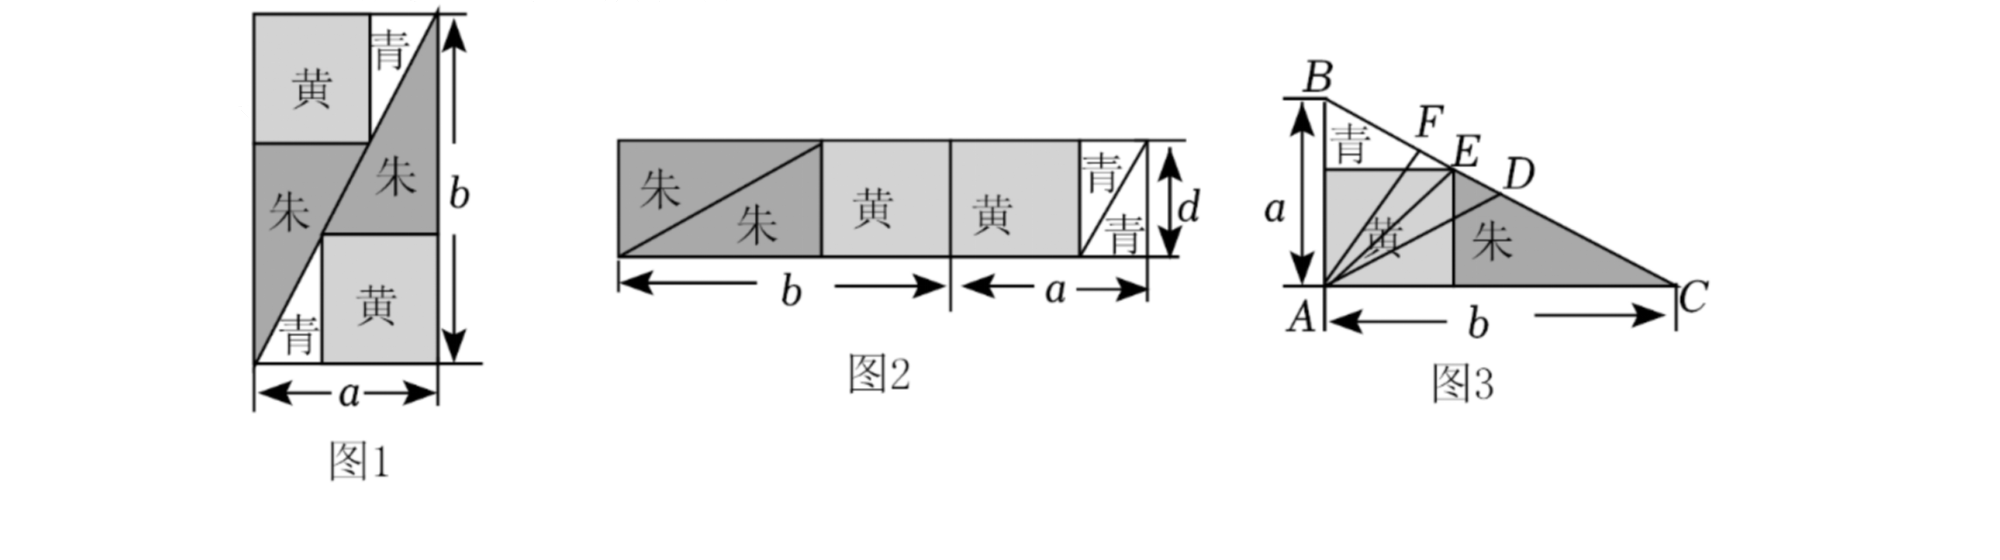
\includegraphics[width=0.86\textwidth]{figures/gao107_q11.png}
\end{center}

①由图 1 和图 2 面积相等得 $d=\dfrac{2ab}{a+b}$　　②由 $AE\geqslant AF$ 可得 $\sqrt{\dfrac{a^2+b^2}2}\geqslant\dfrac{a+b}2$

③由 $AD\geqslant AE$ 可得 $\sqrt{\dfrac{a^2+b^2}2}\geqslant\dfrac{2}{\dfrac1a+\dfrac1b}$　④由 $AD\geqslant AF$ 可得 $a^2+b^2\geqslant2ab$

\ifanswer
\solbegin
\step{对于①，由图 1 和图 2 面积相等得 $ab=(a+b)\times d$，所以 $d=\dfrac{ab}{a+b}$，故①错,}
\step{对于②，因为 $AF\perp BC$，所以 $\dfrac12ab=\dfrac12\sqrt{a^2+b^2}\times AF$,}
\step{所以 $AF=\dfrac{ab}{\sqrt{a^2+b^2}}$，$AE=\sqrt2d=\dfrac{\sqrt2ab}{a+b}$,}
\step{因为 $AE\geqslant AF$，所以 $\dfrac{\sqrt2ab}{a+b}\geqslant\dfrac{ab}{\sqrt{a^2+b^2}}$，整理得 $\sqrt{\dfrac{a^2+b^2}2}\geqslant\dfrac{a+b}2$，故②对,}
\step{对于③，因为 $D$ 是斜边 $BC$ 的中点，所以 $AD=\sqrt{\dfrac{a^2+b^2}2}$,}
\step{因为 $AD\geqslant AE$，所以 $\sqrt{\dfrac{a^2+b^2}2}\geqslant\dfrac{\sqrt2ab}{a+b}$，整理得 $\sqrt{\dfrac{a^2+b^2}2}\geqslant\dfrac{2}{\dfrac1a+\dfrac1b}$，故③对,}
\step{对于④，因为 $AD\geqslant AF$，所以 $\sqrt{\dfrac{a^2+b^2}2}\geqslant\dfrac{ab}{\sqrt{a^2+b^2}}$，整理得 $a^2+b^2\geqslant2ab$,}
\step{故④对,}
\step{故正确的是②③④.}
\solend
\fi

\item 设 $a,b,c,d\in\R$ 且$\lvert a-b\rvert\leqslant2$,$\lvert c-d\rvert\leqslant2$,$\lvert a\rvert\leqslant3$,$\lvert c\rvert\leqslant3$，则 $\lvert ad-bc\rvert$ 的最大值为\blankline[4.4em].% 原卷四处条件间均排半角逗号，照录

\ifanswer
\solbegin
\step{令 $a-b=e$,$c-d=f$，则 $\lvert e\rvert\leqslant2$,$\lvert f\rvert\leqslant2$,$\lvert a\rvert\leqslant3$,$\lvert c\rvert\leqslant3$}
\step{则 $\lvert ad-bc\rvert=\lvert a(c-f)-(a-e)c\rvert=\lvert ce-af\rvert\leqslant\lvert c\rvert\,\lvert e\rvert+\lvert a\rvert\,\lvert f\rvert\leqslant12$,}
\step{则 $\lvert ad-bc\rvert$ 的最大值为 12.}
\solend
\fi

\end{enumerate}

\bigsec{二、选择题}

\begin{enumerate}
\setcounter{enumi}{12}

\item 下列说法正确的是\mbox{（\quad）}

\keepwithprev
A. 若 $a>b>0$，则 $ac^2>bc^2$\qquad\qquad B. 若 $a<b<0$，则 $a^2>ab>b^2$

C. 若 $a>b$，则 $a^2>b^2$\qquad\qquad\qquad D. 若 $a<b$，则 $\dfrac1a>\dfrac1b$

\ifanswer
\solbegin
\step{$A$. 当 $a>b>0$ 时，取 $c=0$，则 $ac^2>bc^2$ 不成立，故 $A$ 错误；}
\step{$B$. 当 $a<b<0$ 时，由不等式的基本性质得 $a^2>ab>b^2>0$，故 $B$ 正确；}
\step{$C$. 当 $a>b$ 时，取 $a=0$，$b=-1$，则 $a^2>b^2$ 不成立，故 $C$ 错误；}
\step{$D$. 当 $a<b$ 时，取 $a=0$，$b=1$，则 $\dfrac1a>\dfrac1b$ 不成立，故 $D$ 错误.}
\step{故选 $B$.}
\solend
\fi

\item 小玲在学习《论语·子路》读到“其身正，不令而行；其身不正，虽令不从”，这句话的
数学含义可以理解为：“身正”是“令行”的\mbox{（\quad）}

\keepwithprev
A. 充分非必要条件\qquad\qquad B. 必要不充分条件

C. 充要条件\qquad\qquad\qquad D. 既非充分又非必要条件

\ifanswer
\solbegin
\step{其身正，不令而行，即身正$\Rightarrow$令行，所以“身正”是“令行”的充分条件；}
\step{又其身不正，虽令不从，即令行$\Rightarrow$身正，所以“身正”是“令行”的必要条件；}
\step{综上，“身正”是“令行”的充要条件. 故选 $C$.}
\solend
\fi

\item 某地对农户抽样调查，结果如下：电冰箱拥有率为 $45\%$，电视机拥有率为 $55\%$，洗衣
机拥有率为 $65\%$，拥有上述三种电器的任意两种的占 $35\%$，三种电器齐全的为 $25\%$，那
么一种电器也没有的农户所占比例是\mbox{（\quad）}

\keepwithprev
A. $12\%$\qquad B. $15\%$\qquad C. $18\%$\qquad D. $20\%$

\ifanswer
\solbegin
\step{设只有电冰箱和电视机的农户有 $a$ 家，只有电冰箱和洗衣机的农户有 $b$ 家,}
\step{只有洗衣机和电视机的农户有 $c$ 家,}
\step{只有电视机、电冰箱、洗衣机的分别有 $d$、$e$、$f$ 家,}
\step{没有任何电器的农户有 $x$ 家,}

\begin{center}
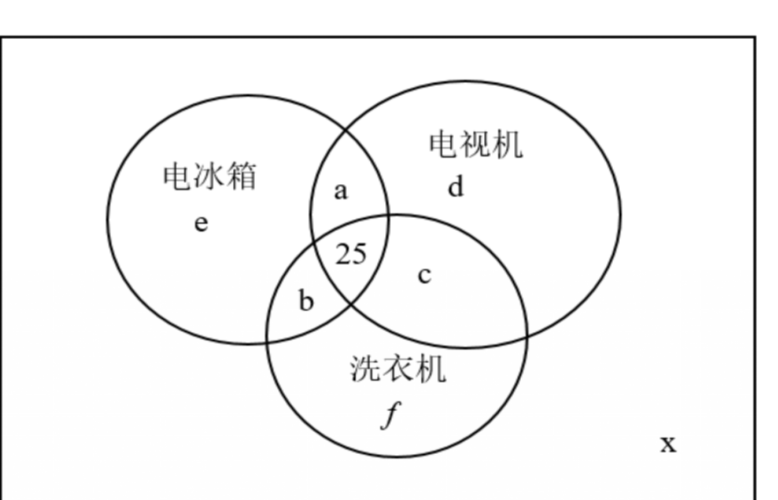
\includegraphics[width=0.42\textwidth]{figures/gao107_q15.png}
\end{center}

\step{所以 $25+a+b+e=45$①，$25+a+c+d=55$②,}
\step{$25+b+c+f=65$③,}
\step{把上面三个式子相加得 $2(a+b+c)+d+e+f=90$④,}
\step{对于拥有上述三种电器的任意两种的占 $35\%$，得 $a+b+c=35$⑤,}
\step{把⑤代入④可得到 $d+e+f=20$⑥,}
\step{因为农户共有 100 家，所以 $25+a+b+c+d+e+f+x=100$,}
\step{把⑤和⑥代入上式得 $x=20$，即一种电器也没有的农户所占比例为 $20\%$.}
\step{故选 $D$.}
\solend
\fi

\item 设 $d>0$，已知 $A,B$ 是两个数集. 若对任意 $x\in A$，都存在 $y\in B$，使得 $\lvert x-y\rvert<d$，则
称 $A$ 是 $B$ 的一个“$d-$邻集”. 现有下列两个命题：① $M=\{a+b\sqrt2\mid a,b\in\Z\}$ 是 $\Q$ 的一个
$\dfrac1{2025}$
一邻集；②若 $A$ 是 $B$ 的一个 $d-$邻集，则 $B$ 也是 $A$ 的一个 $d-$邻集；则\mbox{（\quad）}% 原卷把 d−邻集 的连字符断行后排成“一邻集”，照录

\keepwithprev
A. ①真②假\qquad B. ①假②真\qquad C. ①真②真\qquad D. ①假②假

\ifanswer
\solbegin
\step{对于①，任取 $M$ 中的元素 $x_0=a_0+b_0\sqrt2$,}
\step{则存在 $y_0\in\Q\cap\left(a_0+b_0\sqrt2-\dfrac1{2025},a_0+b_0\sqrt2+\dfrac1{2025}\right)$ 满足题意，故①正确；}
\step{对于②，取 $A=[-1,1]$,$B=[-2,2]$, $A$ 是 $B$ 的 $\dfrac12-$邻集，但反之不成立,}
\step{故②错误；}
\step{故选 $A$.}
\solend
\fi

\end{enumerate}

\bigsec{三、解答题}

\begin{enumerate}
\setcounter{enumi}{16}

\item 设 $a\in\R$，完成下列问题：

（1）求不等式 $3(a+1)x-3>2ax-3a$ 的解集 $M$；

（2）设集合 $A=\{x\mid x^2-ax+a^2-19=0\}$，$B=\{x\mid x^2-5x+6=0\}$，
$C=\{x\mid x^2+2x-8=0\}$. 若 $A\cap B\supset\varnothing$，$A\cap C=\varnothing$，求 $a$ 的值.

\ifanswer
\solbegin
\step{（1）不等式 $3(a+1)x-3>2ax-3a$ 可化为 $(a+3)x>3-3a$,}
\step{当 $a+3>0$，即 $a>-3$ 时，解得 $x>\dfrac{3-3a}{a+3}$,}
\step{当 $a+3=0$，即 $a=-3$ 时，不等式化为 $0\cdot x>12$，无解,}
\step{当 $a+3<0$，即 $a<-3$ 时，解得 $x<\dfrac{3-3a}{a+3}$,}
\step{综上所述，当 $a>-3$ 时，$M=\left(\dfrac{3-3a}{a+3},+\infty\right)$；}
\step{当 $a=-3$ 时，$M=\varnothing$；}
\step{当 $a<-3$ 时，$M=\left(-\infty,\dfrac{3-3a}{a+3}\right)$；}
\step{（2）$B=\{x\mid x^2-5x+6=0\}=\{2,3\}$，$C=\{x\mid x^2+2x-8=0\}=\{2,-4\}$,}
\step{因为 $A\cap B\supset\varnothing$，所以 $A\cap B\neq\varnothing$，又因为 $A\cap C=\varnothing$,}
\step{所以 $3\in A$，$2\notin A$，$-4\notin A$,}
\step{把 $x=3$ 代入方程 $x^2-ax+a^2-19=0$ 得 $9-3a+a^2-19=0$,}
\step{解得 $a=-2$ 或 $a=5$,}
\step{当 $a=-2$ 时，集合 $A=\{x\mid x^2+2x-15=0\}=\{3,-5\}$，符合题意,}
\step{当 $a=5$ 时，集合 $A=\{x\mid x^2-5x+6=0\}=\{3,2\}$，不符合题意，舍去,}
\step{综上所述，$a$ 的值为 $-2$.}
\solend
\fi

\item 完成下列问题：

（1）设 $x$、$y\in\R$，且 $x+y>5$，用反证法证明：$x>3$ 或 $y>2$；

（2）设 $x>0$，$a=x+1$，$b=\sqrt{x^2+7x+1}$，求 $\dfrac ba$ 的最大值.

\ifanswer
\solbegin
\step{（1）假设 $x\leqslant3$ 且 $y\leqslant2$，则 $x+y\leqslant3+2=5$，这与已知 $x+y>5$ 矛盾,}
\step{故 $x>3$ 或 $y>2$；}
\step{（2）$x>0$，$a=x+1$，$b=\sqrt{x^2+7x+1}$,}
\step{则 $\dfrac ba=\dfrac{\sqrt{x^2+7x+1}}{x+1}=\sqrt{\dfrac{x^2+7x+1}{x^2+2x+1}}=\sqrt{\dfrac{x^2+2x+1+5x}{x^2+2x+1}}$}
\step{$=\sqrt{1+\dfrac{5x}{x^2+2x+1}}=\sqrt{1+\dfrac{5}{x+\dfrac1x+2}}\leqslant\sqrt{1+\dfrac{5}{2\sqrt{x\cdot\dfrac1x}+2}}=\dfrac32$,}
\step{当且仅当 $x=\dfrac1x$，即 $x=1$ 时取等号，故 $\dfrac ba$ 的最大值为 $\dfrac32$.}
\solend
\fi

\item 已知函数 $f(x)=\lvert2x-a\rvert+a$.

（1）当 $a=2$ 时，求不等式 $f(x)\leqslant6+\lvert x+2\rvert$ 的解集；

（2）设 $g(x)=\lvert2x-1\rvert$，若不等式 $f(x)+g(x)\geqslant3$ 对一切 $x\in\R$ 恒成立，求实数 $a$ 的取值
范围.

\ifanswer
\solbegin
\ansspace*
\step{（1）$a=2$ 时，$f(x)=\lvert2x-2\rvert+2$,}
\step{则 $f(x)\leqslant6+\lvert x+2\rvert\Leftrightarrow\lvert2x-2\rvert+2\leqslant6+\lvert x+2\rvert$，即 $\lvert2x-2\rvert-\lvert x+2\rvert\leqslant4$,}
\step{当 $x<-2$ 时，$2-2x+x+2\leqslant4$，解得 $x\geqslant0$，与 $x<-2$ 取交集得 $\varnothing$,}
\step{当 $-2\leqslant x\leqslant1$ 时，$2-2x-x-2\leqslant4$，解得 $x\geqslant-\dfrac43$,}
\step{与 $-2\leqslant x\leqslant1$ 取交集得 $-\dfrac43\leqslant x\leqslant1$,}
\step{当 $x>1$ 时，$2x-2-x-2\leqslant4$，解得 $x\leqslant8$，与 $x>1$ 取交集得 $1<x\leqslant8$,}
\step{综上，不等式 $f(x)\leqslant6+\lvert x+2\rvert$ 的解集为 $\left\{x\,\middle|\,-\dfrac43\leqslant x\leqslant8\right\}$；}
\step{（2）$f(x)+g(x)\geqslant3$，即 $\lvert2x-a\rvert+a+\lvert2x-1\rvert\geqslant3$,}
\step{故 $\lvert2x-a\rvert+\lvert2x-1\rvert\geqslant3-a$,}
\step{当 $a\geqslant3$ 时，不等式显然成立,}
\step{当 $a<3$ 时,}
\step{由三角不等式得 $\lvert2x-a\rvert+\lvert2x-1\rvert\geqslant\lvert2x-a-(2x-1)\rvert=\lvert1-a\rvert$,}
\step{当且仅当 $(2x-a)(2x-1)\leqslant0$ 时取等号，因此 $\lvert1-a\rvert\geqslant3-a$,}
\step{平方得 $(1-a)^2\geqslant(3-a)^2$，解得 $a\geqslant2$，故 $2\leqslant a<3$.}
\step{综上，实数 $a$ 的取值范围是 $a\geqslant2$.}
\solend
\fi

\item 对于集合 $A,B$，定义集合 $A-B=\{x\mid x\in A$ 且 $x\notin B\}$.

（1）若 $A=\{1,2,3,4\}$,$B=\{3,4,5\}$，求集合 $A-B$ 和 $B-A$；

（2）给定集合 $A,B$，求所有满足方程组
\[
\begin{cases}
X\cap(A\cup B)=X\\
A\cap(B\cup X)=A\\
B\cap(A\cup X)=B\\
X\cap(A\cap B)=\varnothing
\end{cases}
\]
的集合 $X$（用 $A,B$ 表示）；

（3）用 $\lvert M\rvert$ 表示集合 $M$ 中的元素个数. 给定正整数 $n$，集合 $S=\{1,2,\cdots,n\}$. 对于实数
集的非空有限子集 $A,B$，定义集合 $C=\{x\mid x=a+b,a\in A,b\in B\}$. 求证：

$\lvert A-S\rvert+\lvert B-S\rvert+\lvert S-C\rvert\geqslant1$.

\ifanswer
\solbegin
\step{（1）由 $A=\{1,2,3,4\}$,$B=\{3,4,5\}$，则 $A-B=\{1,2\}$,$B-A=\{5\}$；}
\step{（2）由
$\begin{cases}
X\cap(A\cup B)=X\\
X\cap(A\cap B)=\varnothing
\end{cases}$，
得 $X\subseteq A-B$ 或 $X\subseteq B-A$,}
\step{再结合
$\begin{cases}
A\cap(B\cup X)=A\\
B\cap(A\cup X)=B
\end{cases}$，
得 $X=(A-B)\cup(B-A)$,}
\step{所以 $X=(A-B)\cup(B-A)$；}
\step{（3）$\lvert X\rvert$ 表示集合 $X$ 中的元素个数，则 $\lvert X\rvert\geqslant0$,}
\step{若 $A\cup B$ 中至少含有一个不在 $S$ 中的元素，则 $\lvert A-S\rvert+\lvert B-S\rvert\geqslant1$,}
\step{即 $\lvert A-S\rvert+\lvert B-S\rvert+\lvert S-C\rvert\geqslant1$.}
\step{若 $A\subseteq S$，且 $B\subseteq S$，则 $\lvert A-S\rvert=\lvert B-S\rvert=0$.}
\step{此时 $A$ 中最小的元素 $a\geqslant1$,$B$ 中最小的元素 $b\geqslant1$.}
\step{所以 $C$ 中最小的元素 $a+b\geqslant2$，则 $1\notin C$,}
\step{因为 $S=\{1,2,\cdots,n\}$，所以 $\lvert S-C\rvert\geqslant1$，即 $\lvert A-S\rvert+\lvert B-S\rvert+\lvert S-C\rvert\geqslant1$.}
\step{综上所述，$\lvert A-S\rvert+\lvert B-S\rvert+\lvert S-C\rvert\geqslant1$.}
\solend
\fi

\end{enumerate}

\end{document}
